% Ingeniería de Diseño
% Este archivo se incluye desde main.tex con \input.
\section{Ingeniería de Diseño}
\subsection{Introducción del Capítulo}
El presente capítulo detalla la Ingeniería de Diseño de la solución tecnológica. Tomando como base los requerimientos funcionales y las restricciones operativas definidas en el capítulo anterior, aquí se materializa la arquitectura del software, la estructuración de la base de datos, el diseño de las interfaces de usuario y el modelo de interacciones. El objetivo de este diseño es garantizar que la plataforma sea escalable, segura y capaz de procesar la telemetría concurrente y los modelos de inteligencia artificial de forma eficiente.

\subsection{Diagrama de Sistema de Alto Nivel}
La Figura \ref{fig:arquitectura_alto_nivel} muestra las partes principales de la plataforma y cómo se comunican. El sistema sigue un modelo cliente-servidor con una API REST, y se divide en tres capas, que son la capa de presentación, la capa de procesamiento en la nube y la capa de servicios externos.

\begin{figure}[!htbp]
    \centering
    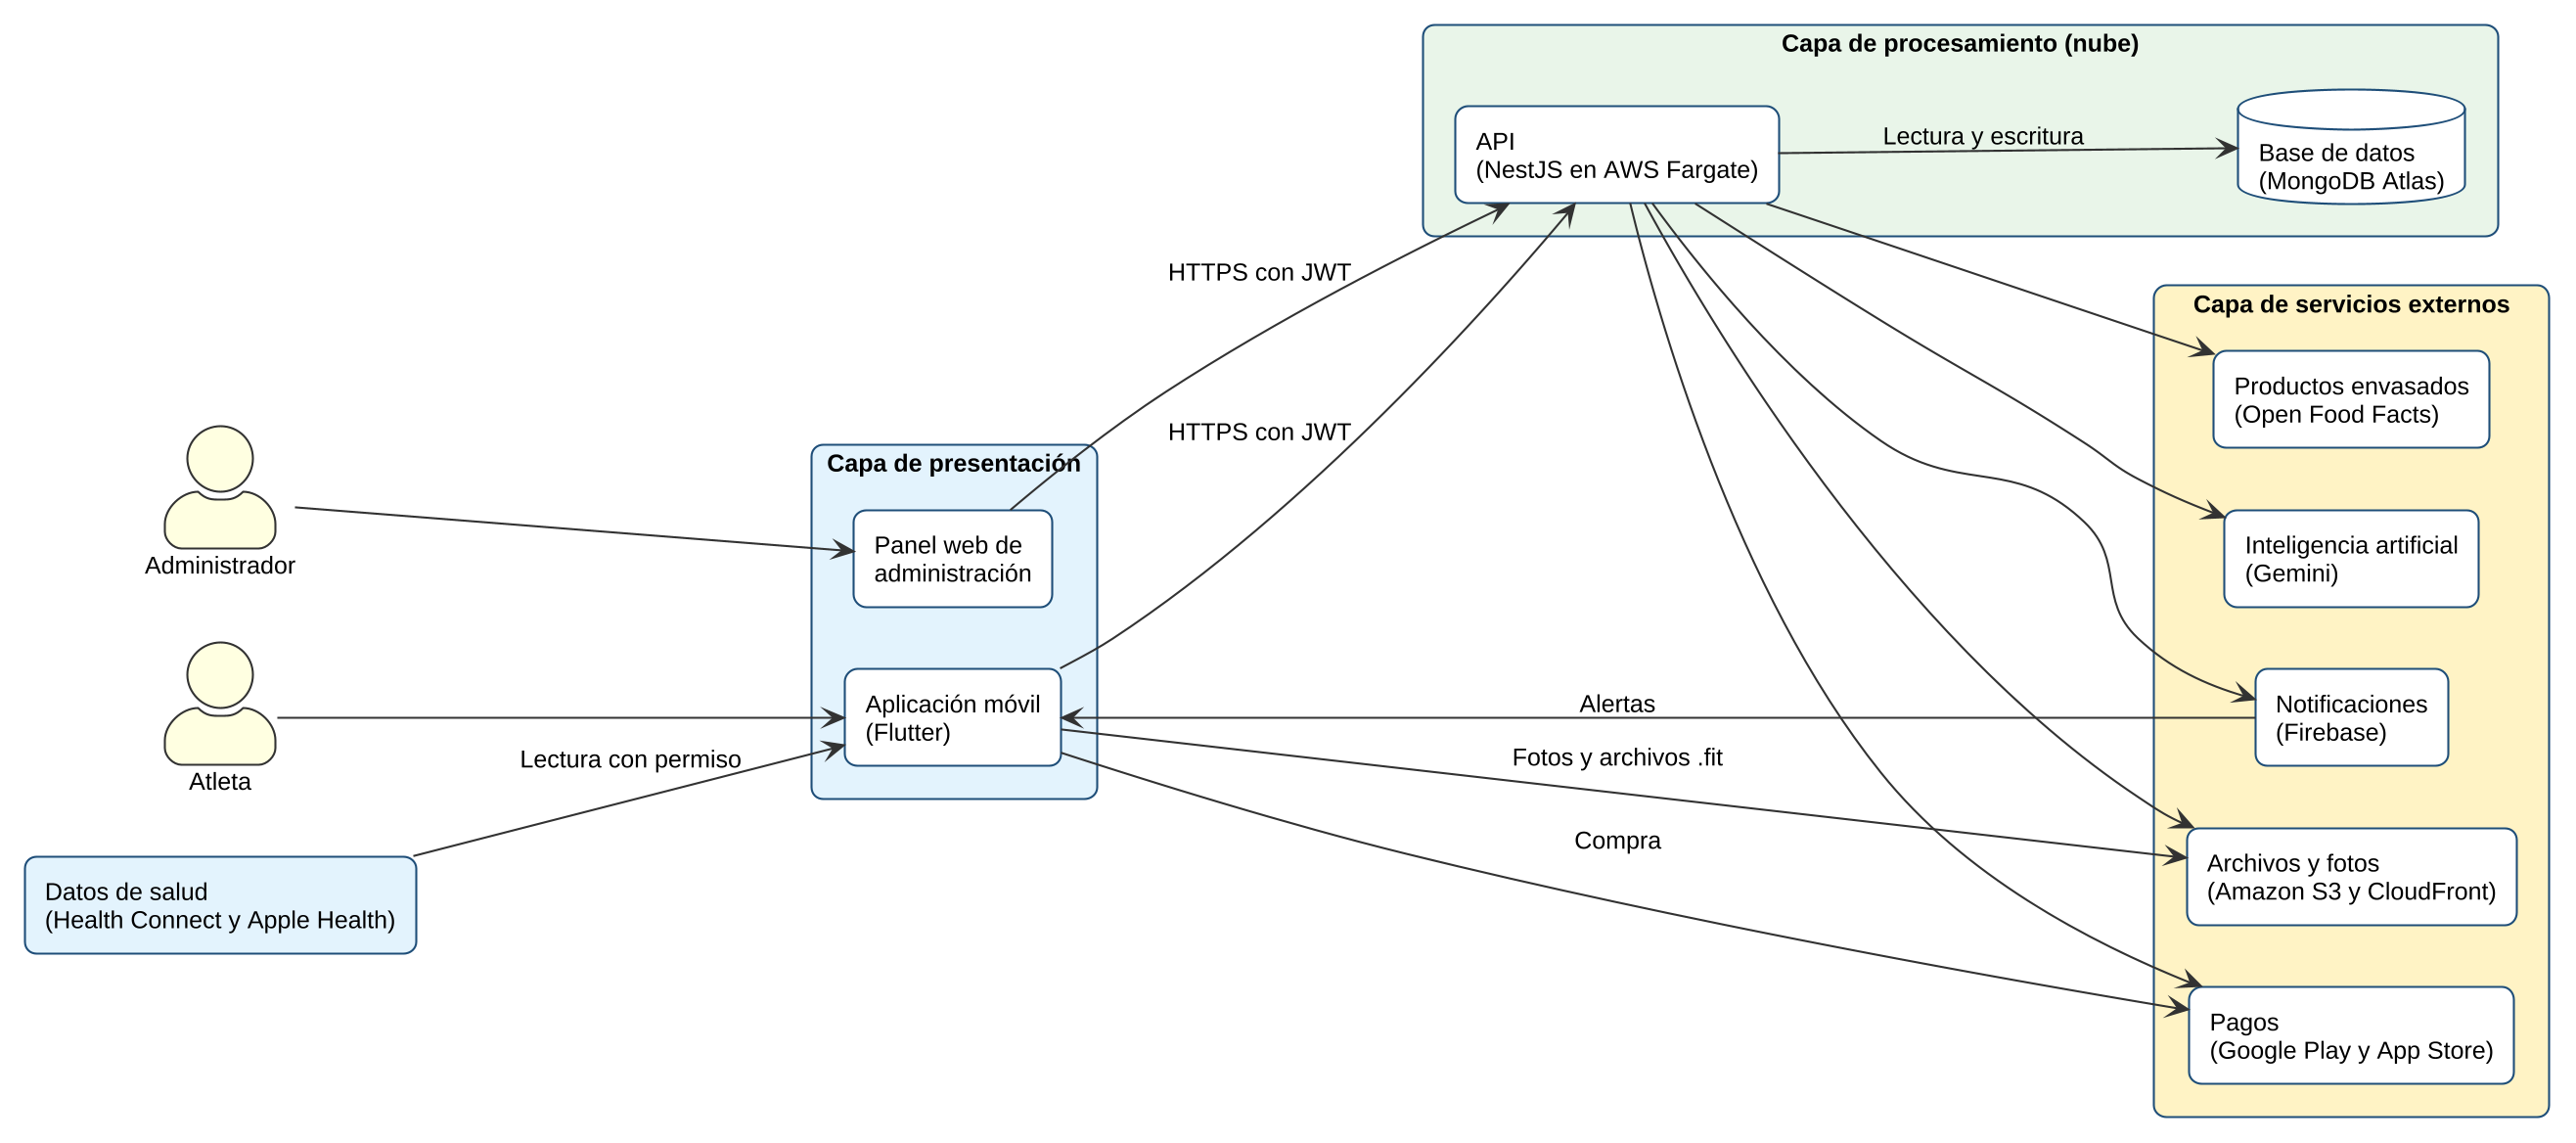
\includegraphics[width=1\textwidth]{figuras/arquitectura/diagrama_arquitectura.png}
    \caption{Arquitectura de Alto Nivel del Sistema.}
    \label{fig:arquitectura_alto_nivel}
\end{figure}
La \textbf{capa de presentación} es lo que usan las personas. El atleta usa la aplicación móvil hecha en \textbf{Flutter}, y el administrador usa un panel web. Además, la aplicación lee, con permiso del usuario, los datos de salud que Health Connect o Apple Health reúnen en el mismo teléfono.

La \textbf{capa de procesamiento} está en la nube. Una API hecha en \textbf{NestJS}, que corre en AWS Fargate, concentra la lógica del sistema, como el cálculo de la fatiga, las metas de alimentación y el plan sugerido. Es la única parte con acceso a la base de datos \textbf{MongoDB}, alojada en MongoDB Atlas, y revisa cada documento antes de guardarlo.

La \textbf{capa de servicios externos} reúne lo que el proyecto no construye por su cuenta. Gemini interpreta las fotos de comida y los textos, Open Food Facts entrega los datos de los productos envasados, Firebase envía las alertas al teléfono, Amazon S3 y CloudFront guardan y muestran los archivos y las fotos, y Google Play y App Store se encargan de los pagos. La mayoría de estas conexiones parte desde la API. Las excepciones son la subida de archivos, la visualización de fotos y el pago, que la aplicación hace directamente. El detalle de cada conexión se explica en la sección Diagrama de Integraciones.
\subsection{Diseño Funcional}
A continuación se presentan los flujos de cada uno de los casos de uso descritos en la fase de requerimientos. Para cada uno se indican sus precondiciones y poscondiciones, su curso normal de eventos y sus cursos alternos. Cada curso alterno lleva el número del paso del curso normal en el que ocurre.

\subsubsection{CU-01. Anotar una sesión de fuerza}

\textbf{Diagrama de Actividades}
\begin{center}
    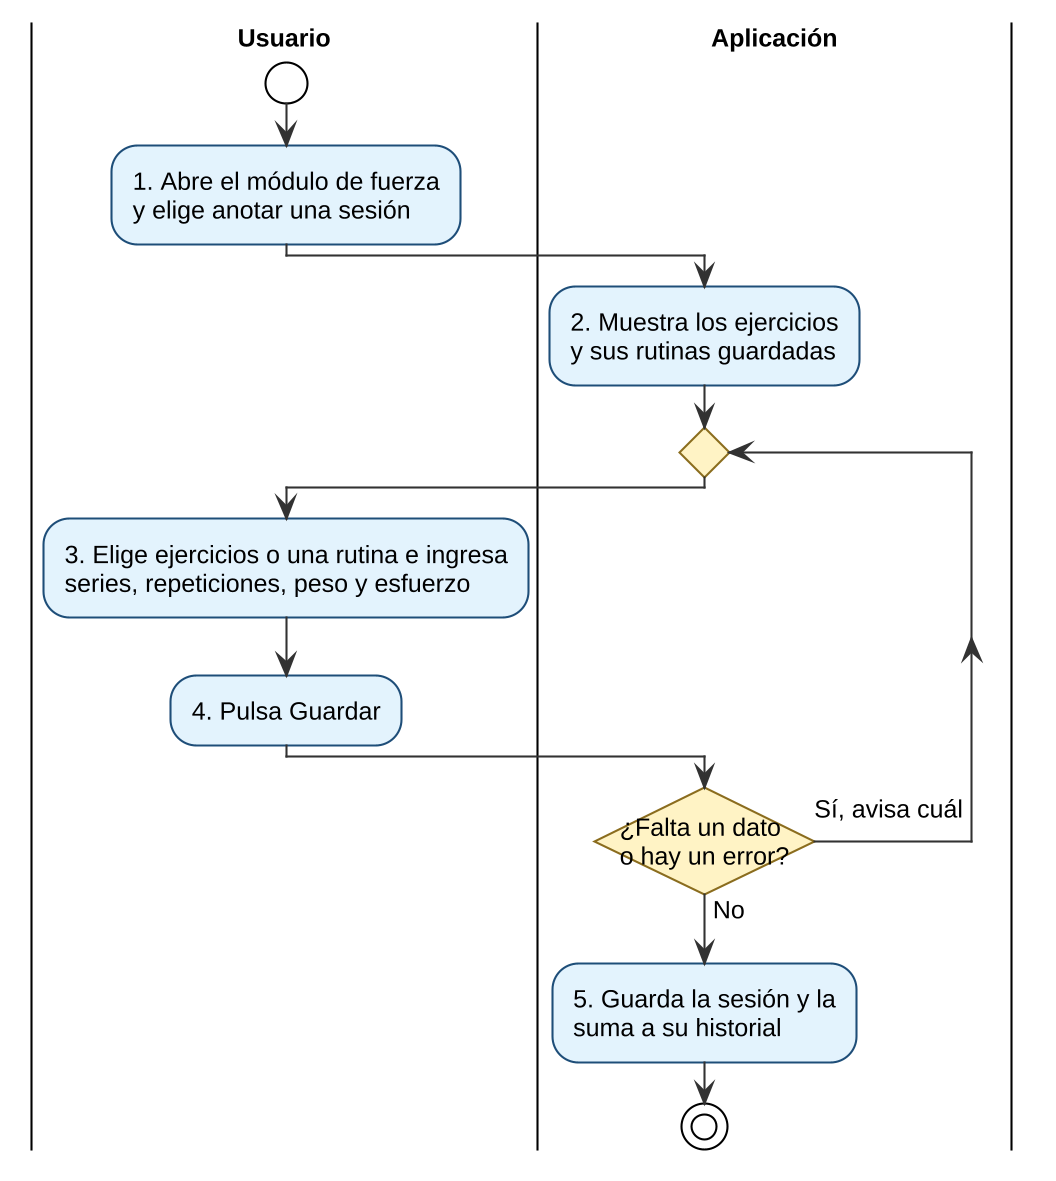
\includegraphics[width=0.78\textwidth,height=0.42\textheight,keepaspectratio]{figuras/diseno/dga_cu01.png}
    \captionof{figure}{Diagrama de Actividades -- CU-01: Anotar una sesión de fuerza.}
    \label{fig:dga_cu01}
\end{center}

\noindent\begin{minipage}{\linewidth}
\textbf{Descripción Esencial Expandida del Caso de Uso}
\par\vspace{0.2cm}
\noindent
{\renewcommand{\arraystretch}{1.25}\setstretch{1}\small
\begin{tabular}{|>{\raggedright\arraybackslash}p{2.9cm}|>{\raggedright\arraybackslash}p{12.1cm}|}
    \hline
    \rowcolor[HTML]{EFEFEF} \textbf{Propósito} & Guardar lo que el atleta hizo en el gimnasio, usando el formulario. \\ \hline
    \textbf{Tipo} & Primario \\ \hline
    \textbf{Actores} & Atleta Básico, Atleta Híbrido \\ \hline
    \textbf{Requerimientos} & R01 \\ \hline
    \textbf{Precondiciones} & El usuario inició sesión en la aplicación. \\ \hline
    \textbf{Poscondiciones} & La sesión queda en el historial del atleta y su carga queda actualizada. \\ \hline
\end{tabular}

\vspace{0.15cm}
\noindent
\begin{tabular}{|>{\raggedright\arraybackslash}p{7.5cm}|>{\raggedright\arraybackslash}p{7.5cm}|}
    \hline
    \rowcolor[HTML]{D9E1F2} \multicolumn{2}{|c|}{\textbf{Curso Normal de los Eventos}} \\ \hline
    \rowcolor[HTML]{EFEFEF} \multicolumn{1}{|c|}{\textbf{Usuario}} & \multicolumn{1}{c|}{\textbf{Respuesta del Sistema}} \\ \hline
        1. Abre el módulo de fuerza y elige anotar una sesión. & 2. Muestra la lista de ejercicios y sus rutinas guardadas. \\ \hline
        3. Elige los ejercicios e ingresa las series, las repeticiones, el peso y qué tan duro lo sintió. &  \\ \hline
        4. Pulsa Guardar. & 5. Revisa que los datos estén completos, guarda la sesión y la suma a su historial. \\ \hline
    \rowcolor[HTML]{F2D9D9} \multicolumn{2}{|c|}{\textbf{Cursos Alternos}} \\ \hline
    \rowcolor[HTML]{EFEFEF} \multicolumn{1}{|c|}{\textbf{Usuario}} & \multicolumn{1}{c|}{\textbf{Respuesta del Sistema}} \\ \hline
        3. Si usa una rutina guardada, los ejercicios ya aparecen y solo completa lo que hizo. &  \\ \hline
         & 5. Si falta un dato o el peso no es un número, avisa cuál es y no guarda hasta que se corrija. \\ \hline
\end{tabular}
}
\end{minipage}
\vspace{0.4cm}

\subsubsection{CU-02. Contar mi sesión de fuerza con mis palabras}

\textbf{Diagrama de Actividades}
\begin{center}
    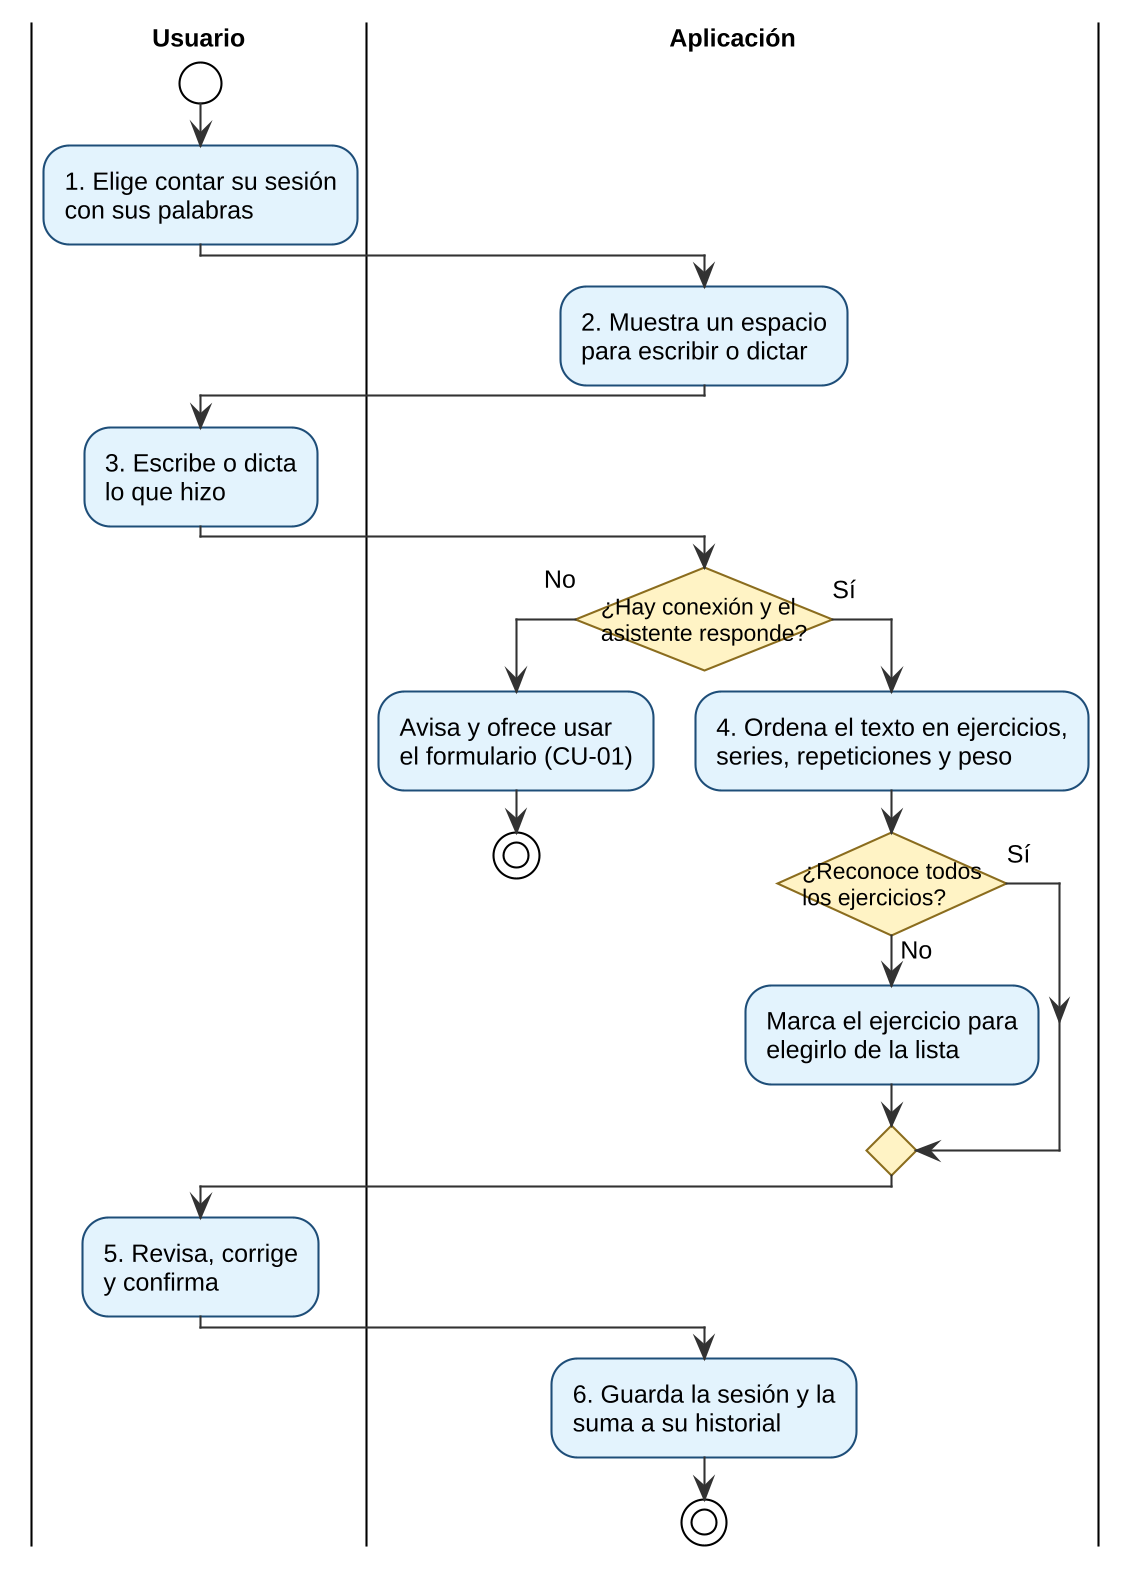
\includegraphics[width=0.78\textwidth,height=0.42\textheight,keepaspectratio]{figuras/diseno/dga_cu02.png}
    \captionof{figure}{Diagrama de Actividades -- CU-02: Contar mi sesión de fuerza con mis palabras.}
    \label{fig:dga_cu02}
\end{center}

\noindent\begin{minipage}{\linewidth}
\textbf{Descripción Esencial Expandida del Caso de Uso}
\par\vspace{0.2cm}
\noindent
{\renewcommand{\arraystretch}{1.25}\setstretch{1}\small
\begin{tabular}{|>{\raggedright\arraybackslash}p{2.9cm}|>{\raggedright\arraybackslash}p{12.1cm}|}
    \hline
    \rowcolor[HTML]{EFEFEF} \textbf{Propósito} & Registrar una sesión de fuerza escribiendo o dictando lo que se hizo, sin llenar un formulario. \\ \hline
    \textbf{Tipo} & Primario \\ \hline
    \textbf{Actores} & Atleta Híbrido, Asistente de inteligencia artificial \\ \hline
    \textbf{Requerimientos} & R01 \\ \hline
    \textbf{Precondiciones} & El usuario inició sesión y tiene el plan premium. Tiene conexión a Internet. \\ \hline
    \textbf{Poscondiciones} & La sesión confirmada queda en el historial del atleta y su carga queda actualizada. \\ \hline
\end{tabular}

\vspace{0.15cm}
\noindent
\begin{tabular}{|>{\raggedright\arraybackslash}p{7.5cm}|>{\raggedright\arraybackslash}p{7.5cm}|}
    \hline
    \rowcolor[HTML]{D9E1F2} \multicolumn{2}{|c|}{\textbf{Curso Normal de los Eventos}} \\ \hline
    \rowcolor[HTML]{EFEFEF} \multicolumn{1}{|c|}{\textbf{Usuario}} & \multicolumn{1}{c|}{\textbf{Respuesta del Sistema}} \\ \hline
        1. Elige contar su sesión con sus palabras. & 2. Muestra un espacio para escribir o dictar. \\ \hline
        3. Escribe o dicta lo que hizo, por ejemplo ``sentadilla, 4 series de 8 con 80 kilos''. & 4. Ordena el texto con ayuda del asistente de IA y muestra los ejercicios, las series, las repeticiones y el peso. \\ \hline
        5. Revisa el resultado, corrige lo que haga falta y lo confirma. & 6. Guarda la sesión y la suma a su historial. \\ \hline
    \rowcolor[HTML]{F2D9D9} \multicolumn{2}{|c|}{\textbf{Cursos Alternos}} \\ \hline
    \rowcolor[HTML]{EFEFEF} \multicolumn{1}{|c|}{\textbf{Usuario}} & \multicolumn{1}{c|}{\textbf{Respuesta del Sistema}} \\ \hline
         & 4. Si no reconoce un ejercicio, lo marca para que el atleta lo elija de la lista. \\ \hline
         & 4. Si no hay conexión o el asistente no responde, avisa y ofrece anotar la sesión con el formulario (CU-01). \\ \hline
\end{tabular}
}
\end{minipage}
\vspace{0.4cm}

\subsubsection{CU-03. Traer mis sesiones desde el reloj}

\textbf{Diagrama de Actividades}
\begin{center}
    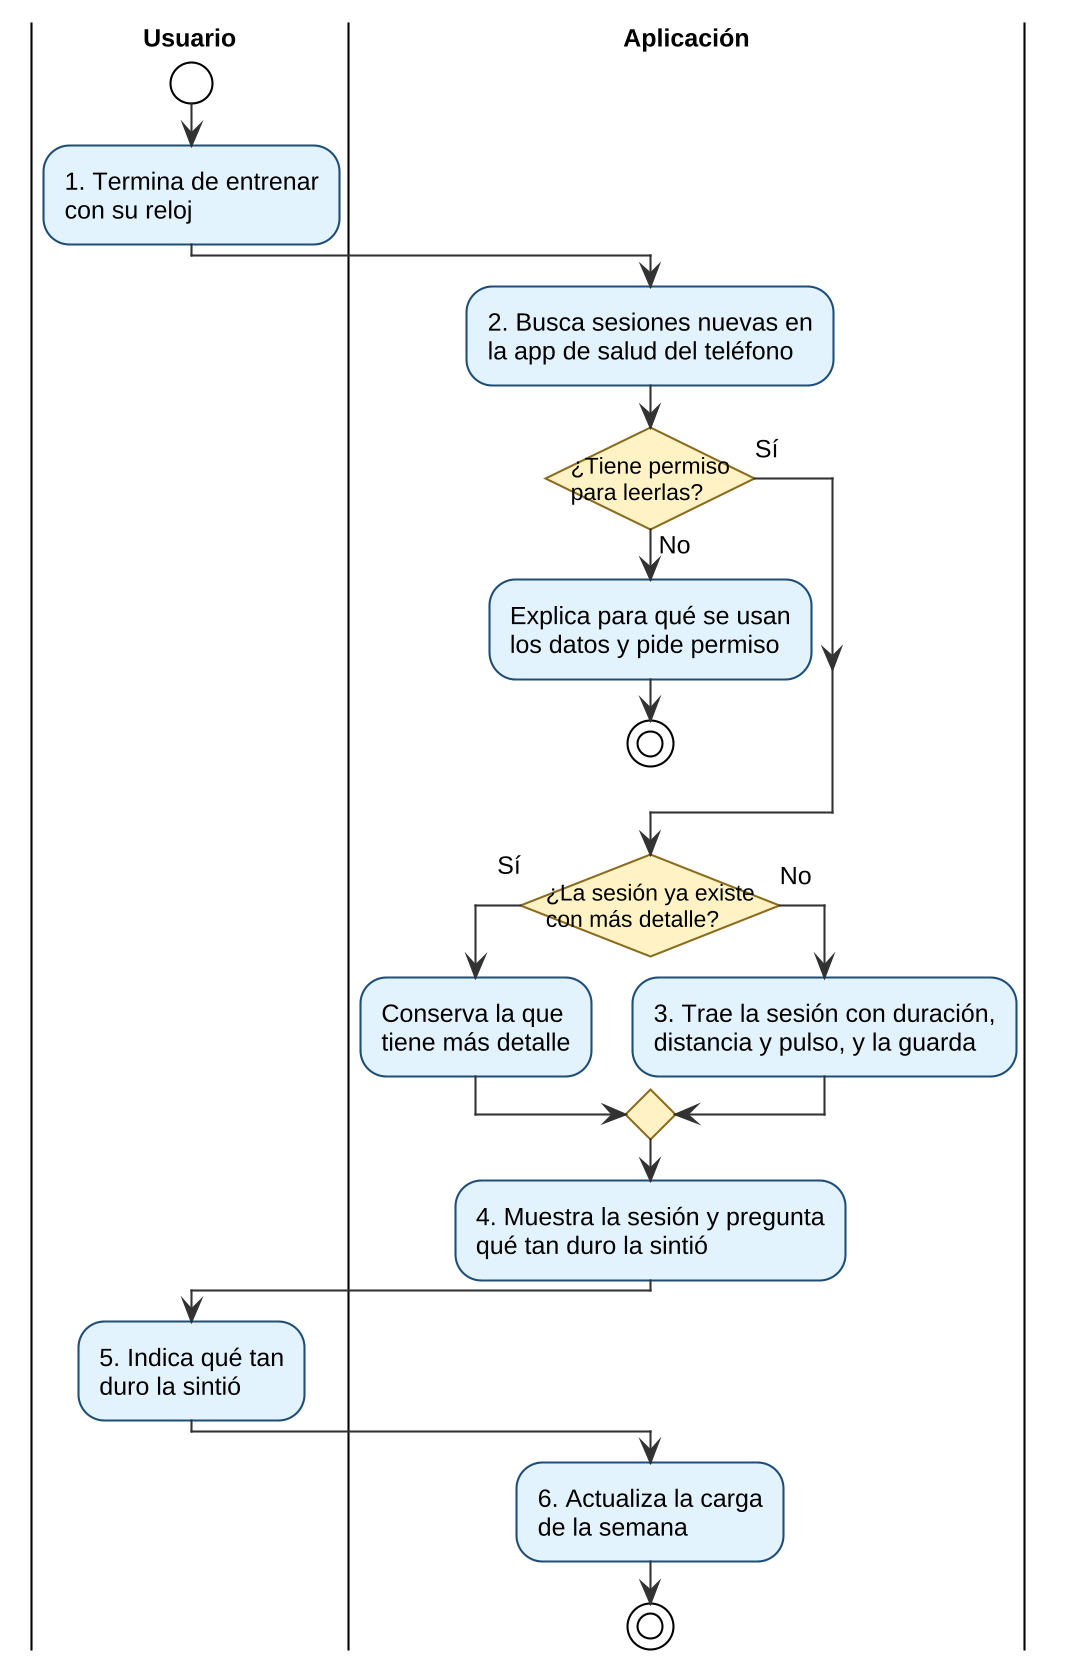
\includegraphics[width=0.78\textwidth,height=0.42\textheight,keepaspectratio]{figuras/diseno/dga_cu03.png}
    \captionof{figure}{Diagrama de Actividades -- CU-03: Traer mis sesiones desde el reloj.}
    \label{fig:dga_cu03}
\end{center}

\noindent\begin{minipage}{\linewidth}
\textbf{Descripción Esencial Expandida del Caso de Uso}
\par\vspace{0.2cm}
\noindent
{\renewcommand{\arraystretch}{1.25}\setstretch{1}\small
\begin{tabular}{|>{\raggedright\arraybackslash}p{2.9cm}|>{\raggedright\arraybackslash}p{12.1cm}|}
    \hline
    \rowcolor[HTML]{EFEFEF} \textbf{Propósito} & Registrar las sesiones de cardio hechas con un reloj, sin anotarlas a mano. \\ \hline
    \textbf{Tipo} & Primario \\ \hline
    \textbf{Actores} & Atleta Híbrido, App de salud del teléfono \\ \hline
    \textbf{Requerimientos} & R02 \\ \hline
    \textbf{Precondiciones} & El usuario inició sesión y tiene el plan premium. Su reloj está conectado a la app de salud del teléfono. \\ \hline
    \textbf{Poscondiciones} & La sesión queda en el historial del atleta y su carga queda actualizada. \\ \hline
\end{tabular}

\vspace{0.15cm}
\noindent
\begin{tabular}{|>{\raggedright\arraybackslash}p{7.5cm}|>{\raggedright\arraybackslash}p{7.5cm}|}
    \hline
    \rowcolor[HTML]{D9E1F2} \multicolumn{2}{|c|}{\textbf{Curso Normal de los Eventos}} \\ \hline
    \rowcolor[HTML]{EFEFEF} \multicolumn{1}{|c|}{\textbf{Usuario}} & \multicolumn{1}{c|}{\textbf{Respuesta del Sistema}} \\ \hline
        1. Termina de entrenar con su reloj. & 2. Busca sesiones nuevas en la app de salud del teléfono. \\ \hline
         & 3. Trae la sesión con su duración, su distancia y su pulso, y la guarda. \\ \hline
         & 4. Muestra la sesión en el historial y pregunta qué tan duro la sintió. \\ \hline
        5. Indica qué tan duro la sintió. & 6. Actualiza la carga de la semana. \\ \hline
    \rowcolor[HTML]{F2D9D9} \multicolumn{2}{|c|}{\textbf{Cursos Alternos}} \\ \hline
    \rowcolor[HTML]{EFEFEF} \multicolumn{1}{|c|}{\textbf{Usuario}} & \multicolumn{1}{c|}{\textbf{Respuesta del Sistema}} \\ \hline
         & 2. Si el atleta aún no da permiso, le explica para qué se usan esos datos y se lo pide. Sin permiso no lee nada. \\ \hline
         & 3. Si la misma sesión ya existe desde un archivo con más detalle, conserva la que tiene más detalle. \\ \hline
        5. Si no responde, la aplicación estima el esfuerzo con su pulso. &  \\ \hline
\end{tabular}
}
\end{minipage}
\vspace{0.4cm}

\subsubsection{CU-04. Subir el archivo de mi ciclocomputador}

\textbf{Diagrama de Actividades}
\begin{center}
    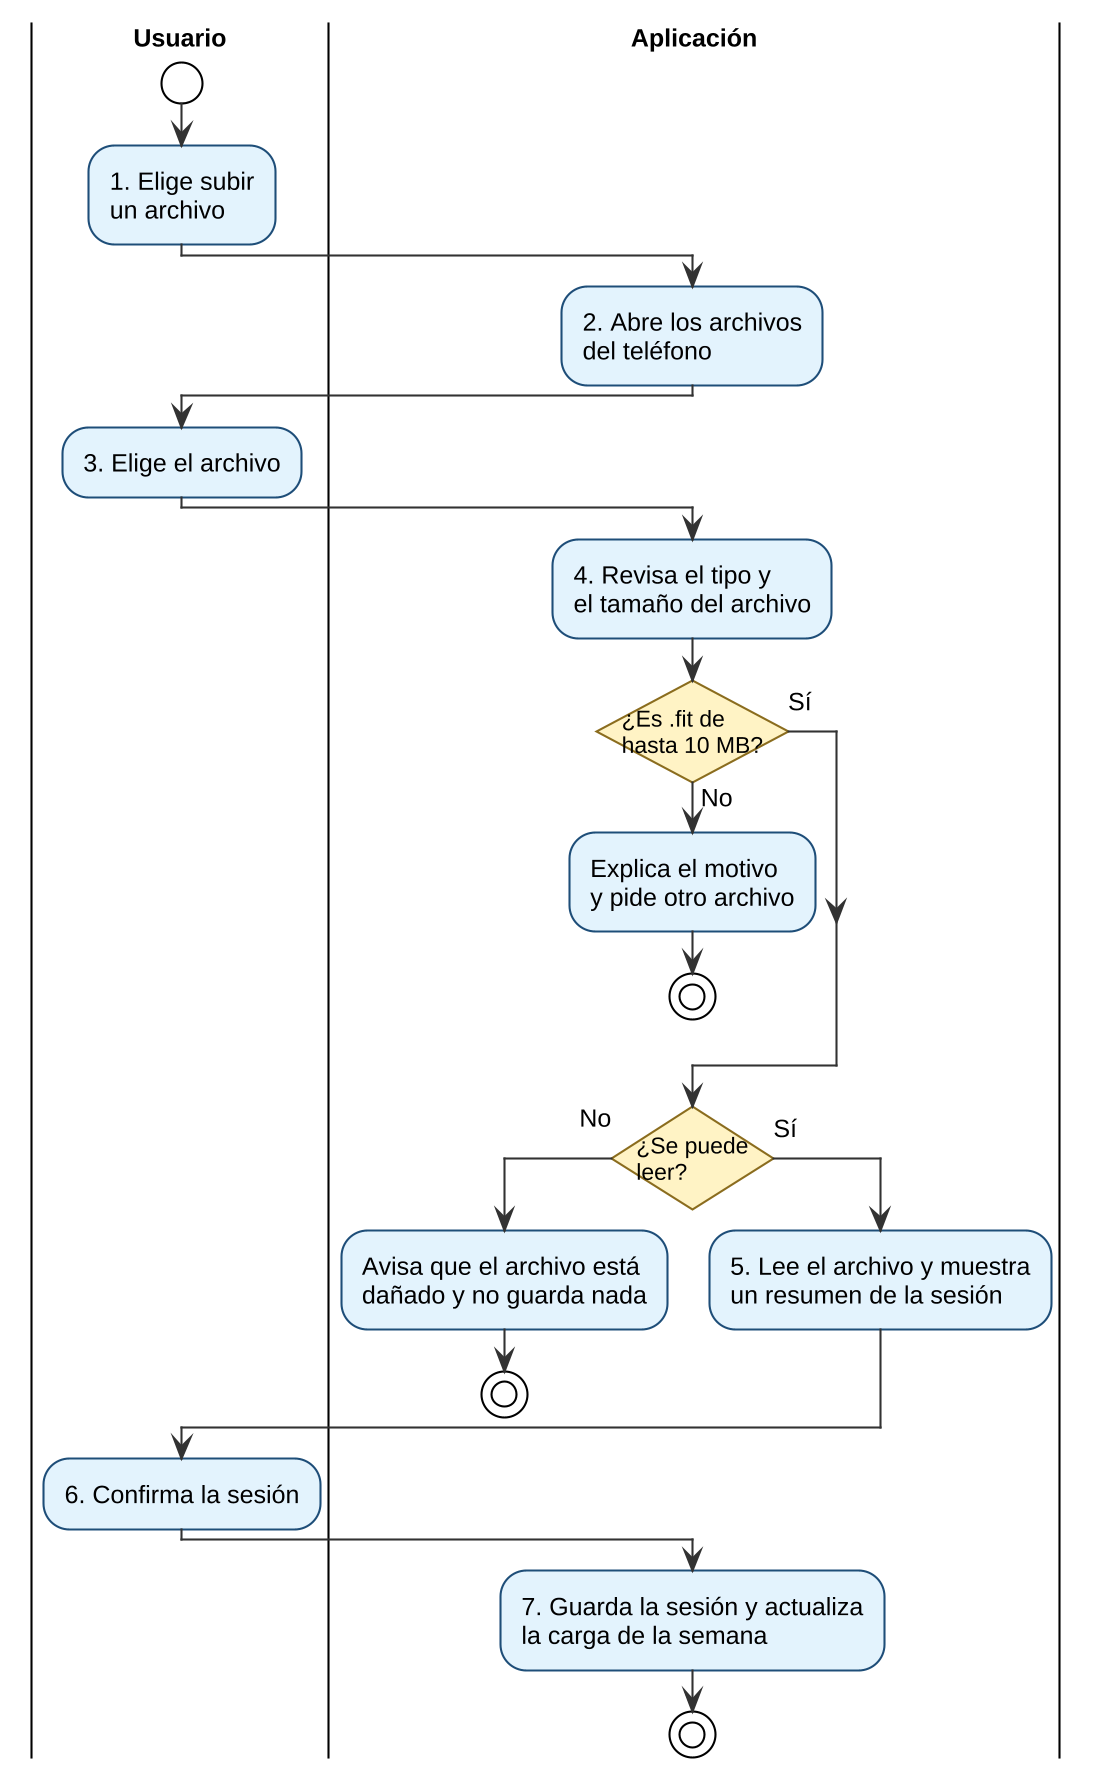
\includegraphics[width=0.78\textwidth,height=0.42\textheight,keepaspectratio]{figuras/diseno/dga_cu04.png}
    \captionof{figure}{Diagrama de Actividades -- CU-04: Subir el archivo de mi ciclocomputador.}
    \label{fig:dga_cu04}
\end{center}

\noindent\begin{minipage}{\linewidth}
\textbf{Descripción Esencial Expandida del Caso de Uso}
\par\vspace{0.2cm}
\noindent
{\renewcommand{\arraystretch}{1.25}\setstretch{1}\small
\begin{tabular}{|>{\raggedright\arraybackslash}p{2.9cm}|>{\raggedright\arraybackslash}p{12.1cm}|}
    \hline
    \rowcolor[HTML]{EFEFEF} \textbf{Propósito} & Incorporar una sesión con todo su detalle, como la potencia y la cadencia. \\ \hline
    \textbf{Tipo} & Primario \\ \hline
    \textbf{Actores} & Atleta Híbrido \\ \hline
    \textbf{Requerimientos} & R02 \\ \hline
    \textbf{Precondiciones} & El usuario inició sesión y tiene el plan premium. Tiene en su teléfono el archivo \texttt{.fit} exportado desde su dispositivo. \\ \hline
    \textbf{Poscondiciones} & La sesión queda en el historial del atleta, con el detalle del archivo. \\ \hline
\end{tabular}

\vspace{0.15cm}
\noindent
\begin{tabular}{|>{\raggedright\arraybackslash}p{7.5cm}|>{\raggedright\arraybackslash}p{7.5cm}|}
    \hline
    \rowcolor[HTML]{D9E1F2} \multicolumn{2}{|c|}{\textbf{Curso Normal de los Eventos}} \\ \hline
    \rowcolor[HTML]{EFEFEF} \multicolumn{1}{|c|}{\textbf{Usuario}} & \multicolumn{1}{c|}{\textbf{Respuesta del Sistema}} \\ \hline
        1. Elige subir un archivo. & 2. Abre los archivos del teléfono. \\ \hline
        3. Elige el archivo. & 4. Revisa que sea un archivo \texttt{.fit} de hasta 10 MB. \\ \hline
         & 5. Lee el archivo y muestra un resumen de la sesión. \\ \hline
        6. Confirma la sesión. & 7. Guarda la sesión y actualiza la carga de la semana. \\ \hline
    \rowcolor[HTML]{F2D9D9} \multicolumn{2}{|c|}{\textbf{Cursos Alternos}} \\ \hline
    \rowcolor[HTML]{EFEFEF} \multicolumn{1}{|c|}{\textbf{Usuario}} & \multicolumn{1}{c|}{\textbf{Respuesta del Sistema}} \\ \hline
         & 4. Si no es un archivo \texttt{.fit} o pesa más de 10 MB, explica el motivo y pide otro archivo. \\ \hline
         & 5. Si el archivo está dañado, avisa que no se pudo leer y no guarda nada. \\ \hline
\end{tabular}
}
\end{minipage}
\vspace{0.4cm}

\subsubsection{CU-05. Revisar mi fatiga y recibir alertas}

\textbf{Diagrama de Actividades}
\begin{center}
    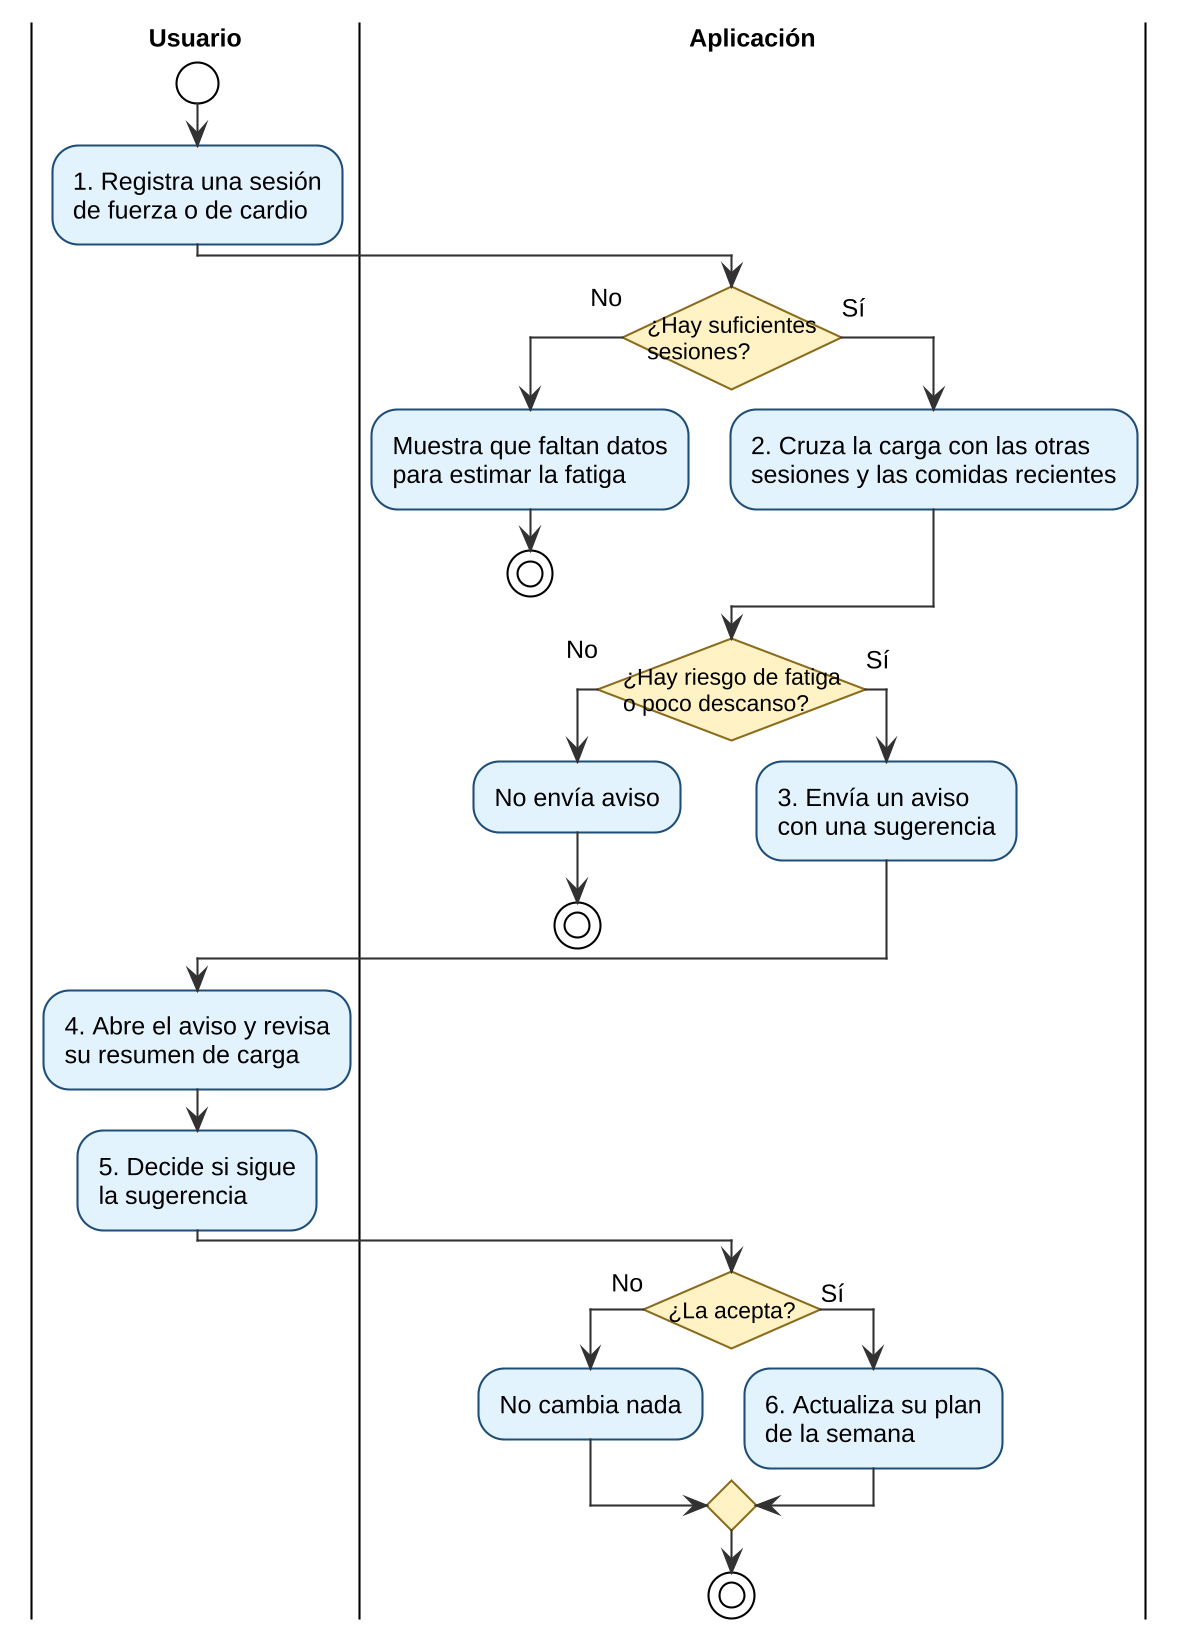
\includegraphics[width=0.78\textwidth,height=0.42\textheight,keepaspectratio]{figuras/diseno/dga_cu05.png}
    \captionof{figure}{Diagrama de Actividades -- CU-05: Revisar mi fatiga y recibir alertas.}
    \label{fig:dga_cu05}
\end{center}

\noindent\begin{minipage}{\linewidth}
\textbf{Descripción Esencial Expandida del Caso de Uso}
\par\vspace{0.2cm}
\noindent
{\renewcommand{\arraystretch}{1.25}\setstretch{1}\small
\begin{tabular}{|>{\raggedright\arraybackslash}p{2.9cm}|>{\raggedright\arraybackslash}p{12.1cm}|}
    \hline
    \rowcolor[HTML]{EFEFEF} \textbf{Propósito} & Avisar al atleta cuando puede estar acumulando demasiada fatiga, para que decida si ajusta su entrenamiento. \\ \hline
    \textbf{Tipo} & Primario \\ \hline
    \textbf{Actores} & Atleta Híbrido \\ \hline
    \textbf{Requerimientos} & R03 \\ \hline
    \textbf{Precondiciones} & El usuario inició sesión y tiene el plan premium. Tiene sesiones registradas. \\ \hline
    \textbf{Poscondiciones} & El atleta conoce su nivel de fatiga. Su entrenamiento solo cambia si él lo decide. \\ \hline
\end{tabular}

\vspace{0.15cm}
\noindent
\begin{tabular}{|>{\raggedright\arraybackslash}p{7.5cm}|>{\raggedright\arraybackslash}p{7.5cm}|}
    \hline
    \rowcolor[HTML]{D9E1F2} \multicolumn{2}{|c|}{\textbf{Curso Normal de los Eventos}} \\ \hline
    \rowcolor[HTML]{EFEFEF} \multicolumn{1}{|c|}{\textbf{Usuario}} & \multicolumn{1}{c|}{\textbf{Respuesta del Sistema}} \\ \hline
        1. Registra una sesión de fuerza o de cardio. & 2. Cruza la carga de la sesión con las otras sesiones y las comidas de los últimos días. \\ \hline
         & 3. Detecta un riesgo de fatiga o de poco descanso y envía un aviso con una sugerencia. \\ \hline
        4. Abre el aviso y revisa su resumen de carga. &  \\ \hline
        5. Decide si sigue la sugerencia. & 6. Si la acepta, actualiza su plan de la semana. \\ \hline
    \rowcolor[HTML]{F2D9D9} \multicolumn{2}{|c|}{\textbf{Cursos Alternos}} \\ \hline
    \rowcolor[HTML]{EFEFEF} \multicolumn{1}{|c|}{\textbf{Usuario}} & \multicolumn{1}{c|}{\textbf{Respuesta del Sistema}} \\ \hline
         & 2. Si todavía hay pocas sesiones, muestra que faltan datos para estimar la fatiga. \\ \hline
         & 3. Si no hay riesgo, no envía aviso. El atleta puede ver su resumen cuando quiera. \\ \hline
        5. Si ignora la sugerencia, la aplicación no cambia nada. &  \\ \hline
\end{tabular}
}
\end{minipage}
\vspace{0.4cm}

\subsubsection{CU-06. Anotar una comida buscando los alimentos}

\textbf{Diagrama de Actividades}
\begin{center}
    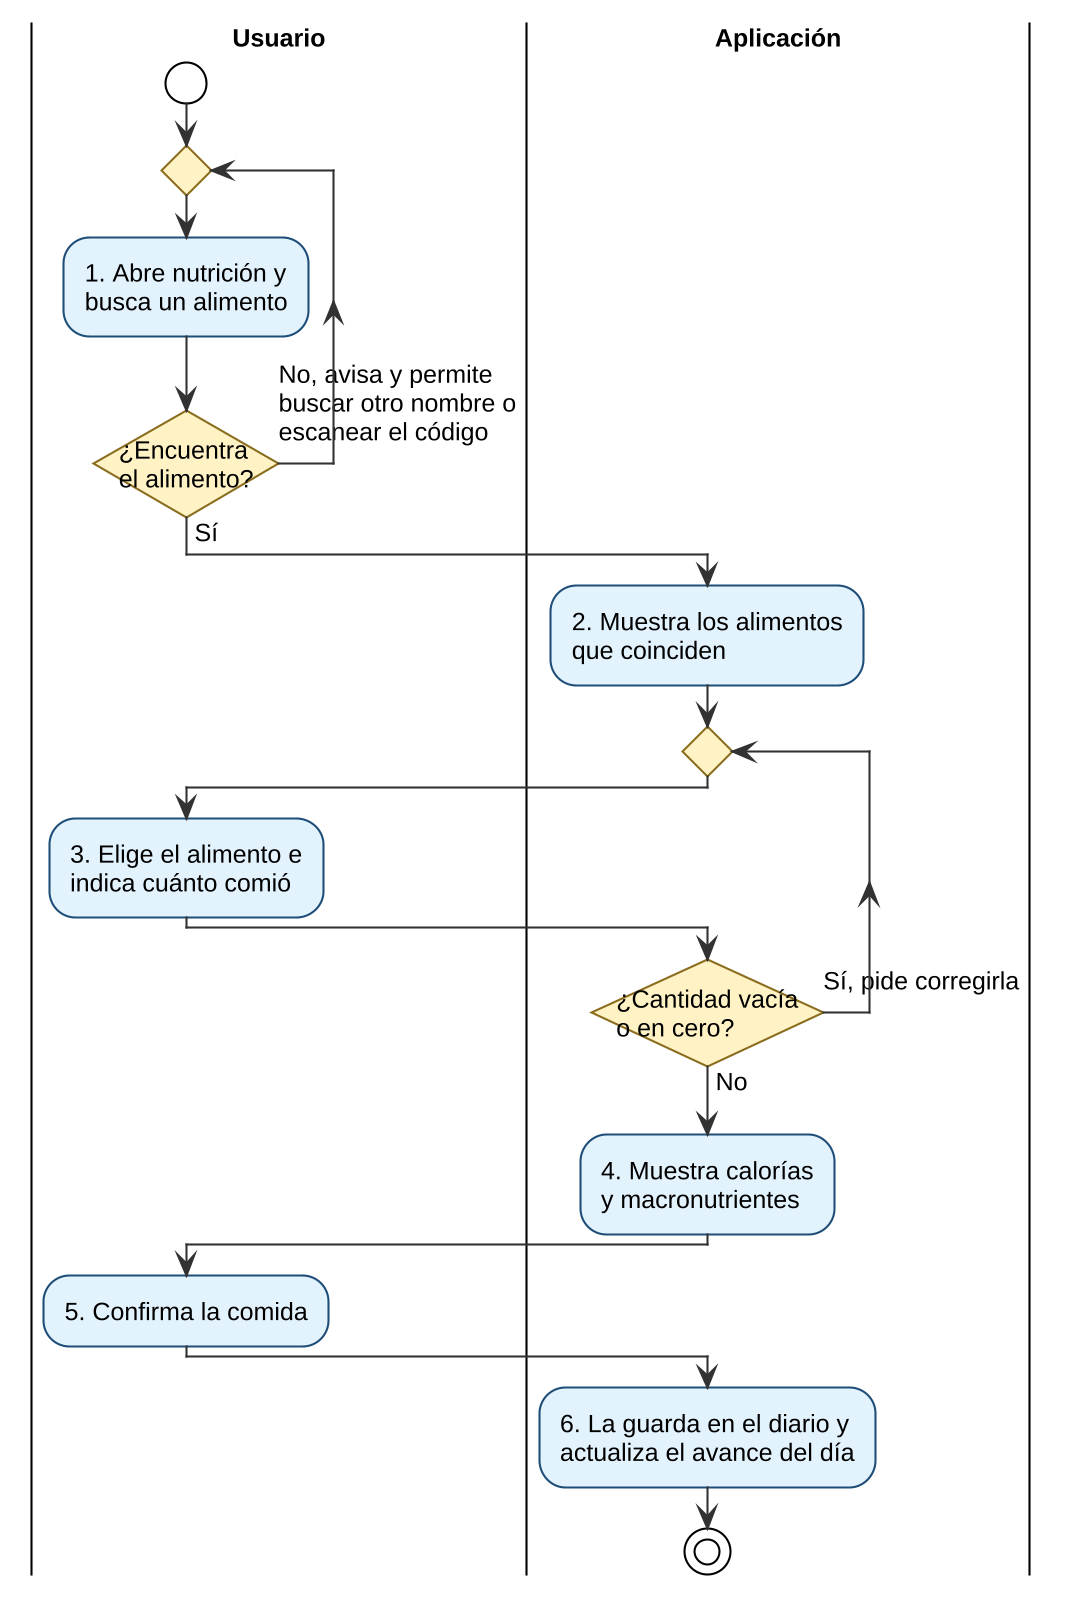
\includegraphics[width=0.78\textwidth,height=0.42\textheight,keepaspectratio]{figuras/diseno/dga_cu06.png}
    \captionof{figure}{Diagrama de Actividades -- CU-06: Anotar una comida buscando los alimentos.}
    \label{fig:dga_cu06}
\end{center}

\noindent\begin{minipage}{\linewidth}
\textbf{Descripción Esencial Expandida del Caso de Uso}
\par\vspace{0.2cm}
\noindent
{\renewcommand{\arraystretch}{1.25}\setstretch{1}\small
\begin{tabular}{|>{\raggedright\arraybackslash}p{2.9cm}|>{\raggedright\arraybackslash}p{12.1cm}|}
    \hline
    \rowcolor[HTML]{EFEFEF} \textbf{Propósito} & Registrar una comida eligiendo los alimentos desde una lista. \\ \hline
    \textbf{Tipo} & Primario \\ \hline
    \textbf{Actores} & Atleta Básico, Atleta Híbrido \\ \hline
    \textbf{Requerimientos} & R04 \\ \hline
    \textbf{Precondiciones} & El usuario inició sesión en la aplicación. \\ \hline
    \textbf{Poscondiciones} & La comida queda en el diario del día. \\ \hline
\end{tabular}

\vspace{0.15cm}
\noindent
\begin{tabular}{|>{\raggedright\arraybackslash}p{7.5cm}|>{\raggedright\arraybackslash}p{7.5cm}|}
    \hline
    \rowcolor[HTML]{D9E1F2} \multicolumn{2}{|c|}{\textbf{Curso Normal de los Eventos}} \\ \hline
    \rowcolor[HTML]{EFEFEF} \multicolumn{1}{|c|}{\textbf{Usuario}} & \multicolumn{1}{c|}{\textbf{Respuesta del Sistema}} \\ \hline
        1. Abre el módulo de nutrición y busca un alimento. & 2. Muestra los alimentos que coinciden. \\ \hline
        3. Elige el alimento e indica cuánto comió. & 4. Muestra sus calorías y sus macronutrientes. \\ \hline
        5. Confirma la comida. & 6. La guarda en el diario y actualiza el avance del día. \\ \hline
    \rowcolor[HTML]{F2D9D9} \multicolumn{2}{|c|}{\textbf{Cursos Alternos}} \\ \hline
    \rowcolor[HTML]{EFEFEF} \multicolumn{1}{|c|}{\textbf{Usuario}} & \multicolumn{1}{c|}{\textbf{Respuesta del Sistema}} \\ \hline
         & 2. Si no encuentra el alimento, avisa y permite buscar con otro nombre o escanear su código de barras (CU-15). \\ \hline
        3. Si la cantidad está vacía o es cero, la aplicación pide corregirla antes de seguir. &  \\ \hline
\end{tabular}
}
\end{minipage}
\vspace{0.4cm}

\subsubsection{CU-07. Registrar una comida con una foto}

\textbf{Diagrama de Actividades}
\begin{center}
    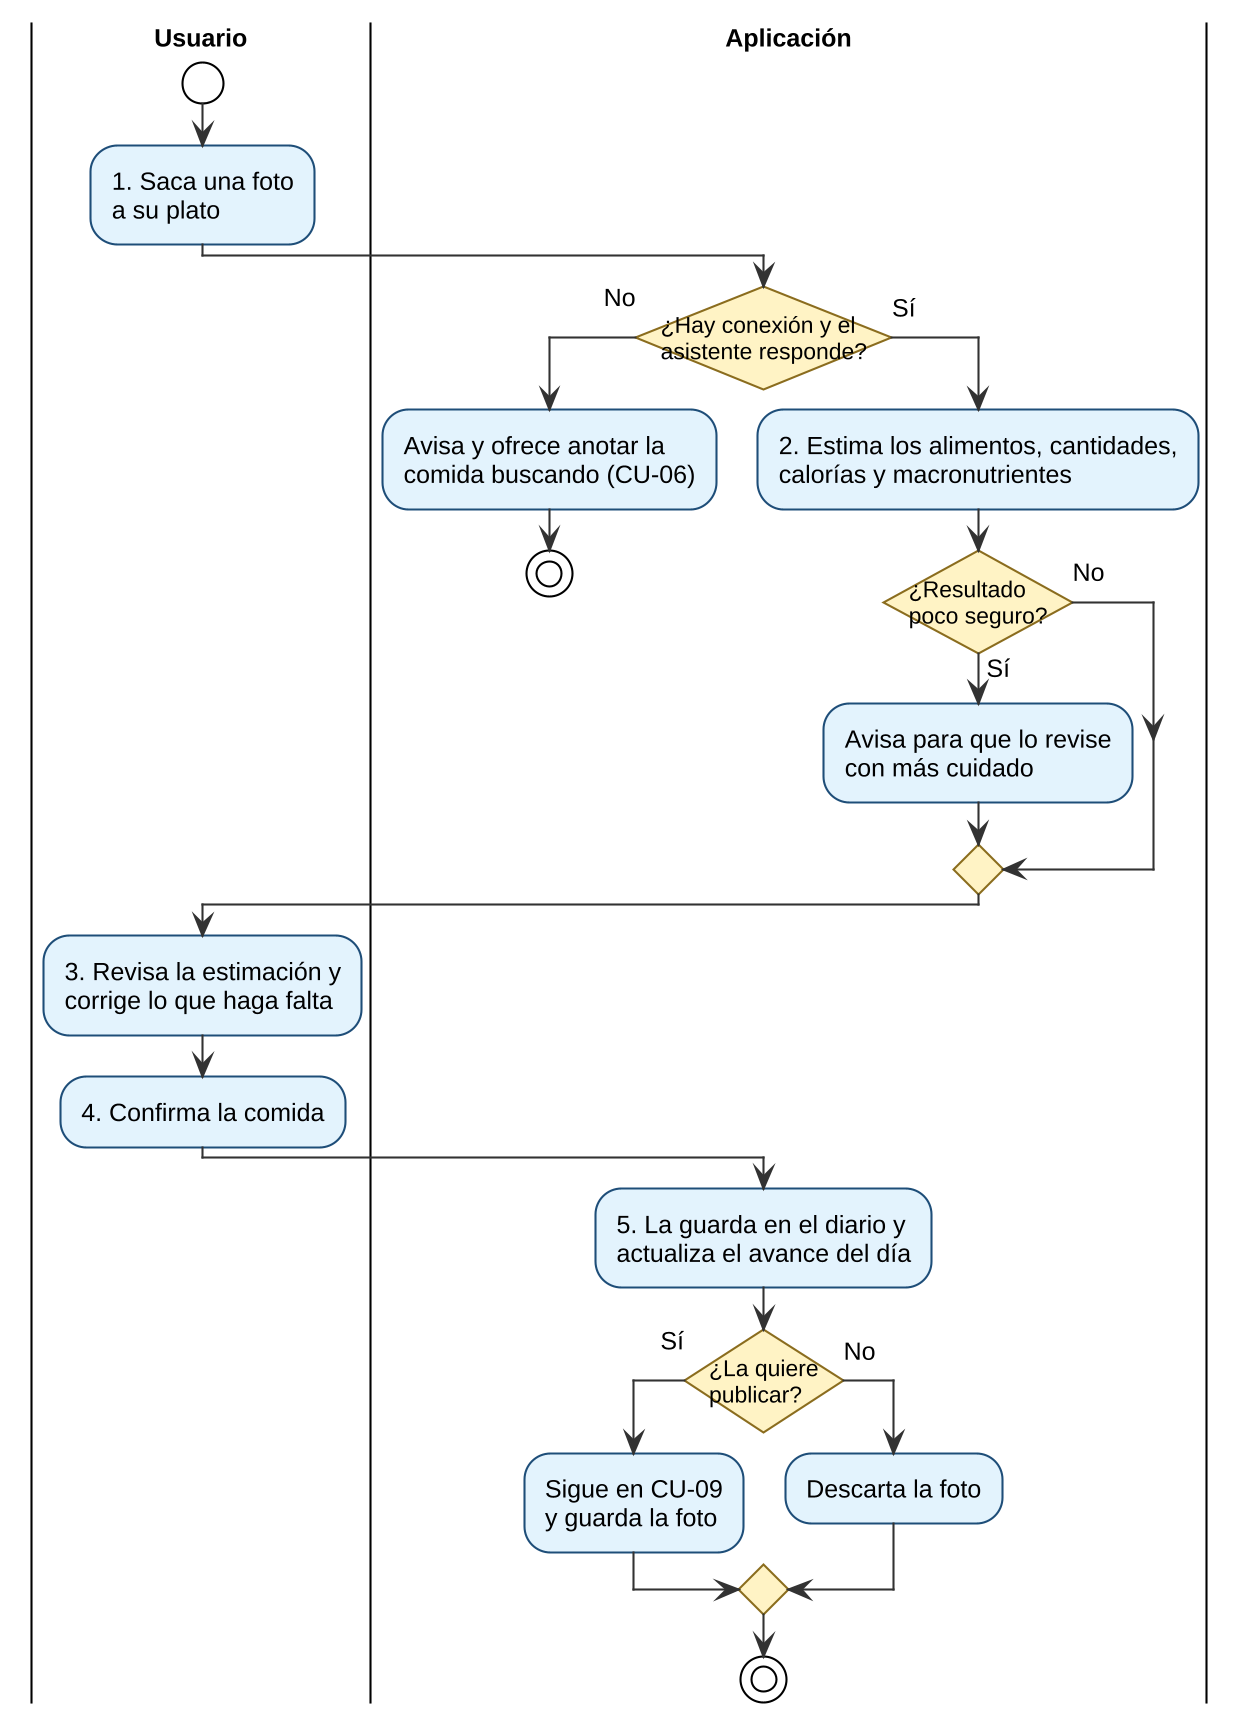
\includegraphics[width=0.78\textwidth,height=0.42\textheight,keepaspectratio]{figuras/diseno/dga_cu07.png}
    \captionof{figure}{Diagrama de Actividades -- CU-07: Registrar una comida con una foto.}
    \label{fig:dga_cu07}
\end{center}

\noindent\begin{minipage}{\linewidth}
\textbf{Descripción Esencial Expandida del Caso de Uso}
\par\vspace{0.2cm}
\noindent
{\renewcommand{\arraystretch}{1.25}\setstretch{1}\small
\begin{tabular}{|>{\raggedright\arraybackslash}p{2.9cm}|>{\raggedright\arraybackslash}p{12.1cm}|}
    \hline
    \rowcolor[HTML]{EFEFEF} \textbf{Propósito} & Registrar una comida sacándole una foto al plato, para no buscar cada alimento. \\ \hline
    \textbf{Tipo} & Primario \\ \hline
    \textbf{Actores} & Atleta Híbrido, Asistente de inteligencia artificial \\ \hline
    \textbf{Requerimientos} & R04 \\ \hline
    \textbf{Precondiciones} & El usuario inició sesión y tiene el plan premium. Tiene conexión a Internet. \\ \hline
    \textbf{Poscondiciones} & La comida confirmada queda en el diario del día. \\ \hline
\end{tabular}

\vspace{0.15cm}
\noindent
\begin{tabular}{|>{\raggedright\arraybackslash}p{7.5cm}|>{\raggedright\arraybackslash}p{7.5cm}|}
    \hline
    \rowcolor[HTML]{D9E1F2} \multicolumn{2}{|c|}{\textbf{Curso Normal de los Eventos}} \\ \hline
    \rowcolor[HTML]{EFEFEF} \multicolumn{1}{|c|}{\textbf{Usuario}} & \multicolumn{1}{c|}{\textbf{Respuesta del Sistema}} \\ \hline
        1. Saca una foto a su plato. & 2. Estima con ayuda del asistente de IA los alimentos, las cantidades, las calorías y los macronutrientes, y los muestra. \\ \hline
        3. Revisa la estimación y corrige lo que haga falta. &  \\ \hline
        4. Confirma la comida. & 5. La guarda en el diario, actualiza el avance del día y descarta la foto. \\ \hline
    \rowcolor[HTML]{F2D9D9} \multicolumn{2}{|c|}{\textbf{Cursos Alternos}} \\ \hline
    \rowcolor[HTML]{EFEFEF} \multicolumn{1}{|c|}{\textbf{Usuario}} & \multicolumn{1}{c|}{\textbf{Respuesta del Sistema}} \\ \hline
         & 2. Si el resultado es poco seguro, avisa al atleta para que lo revise con más cuidado. \\ \hline
         & 2. Si no hay conexión o el asistente no responde, avisa y ofrece anotar la comida buscando los alimentos (CU-06). \\ \hline
        4. Si quiere compartir el plato, puede publicarlo (CU-09). En ese caso la foto sí se guarda. &  \\ \hline
\end{tabular}
}
\end{minipage}
\vspace{0.4cm}

\subsubsection{CU-08. Agregar una receta ajustada a mis metas}

\textbf{Diagrama de Actividades}
\begin{center}
    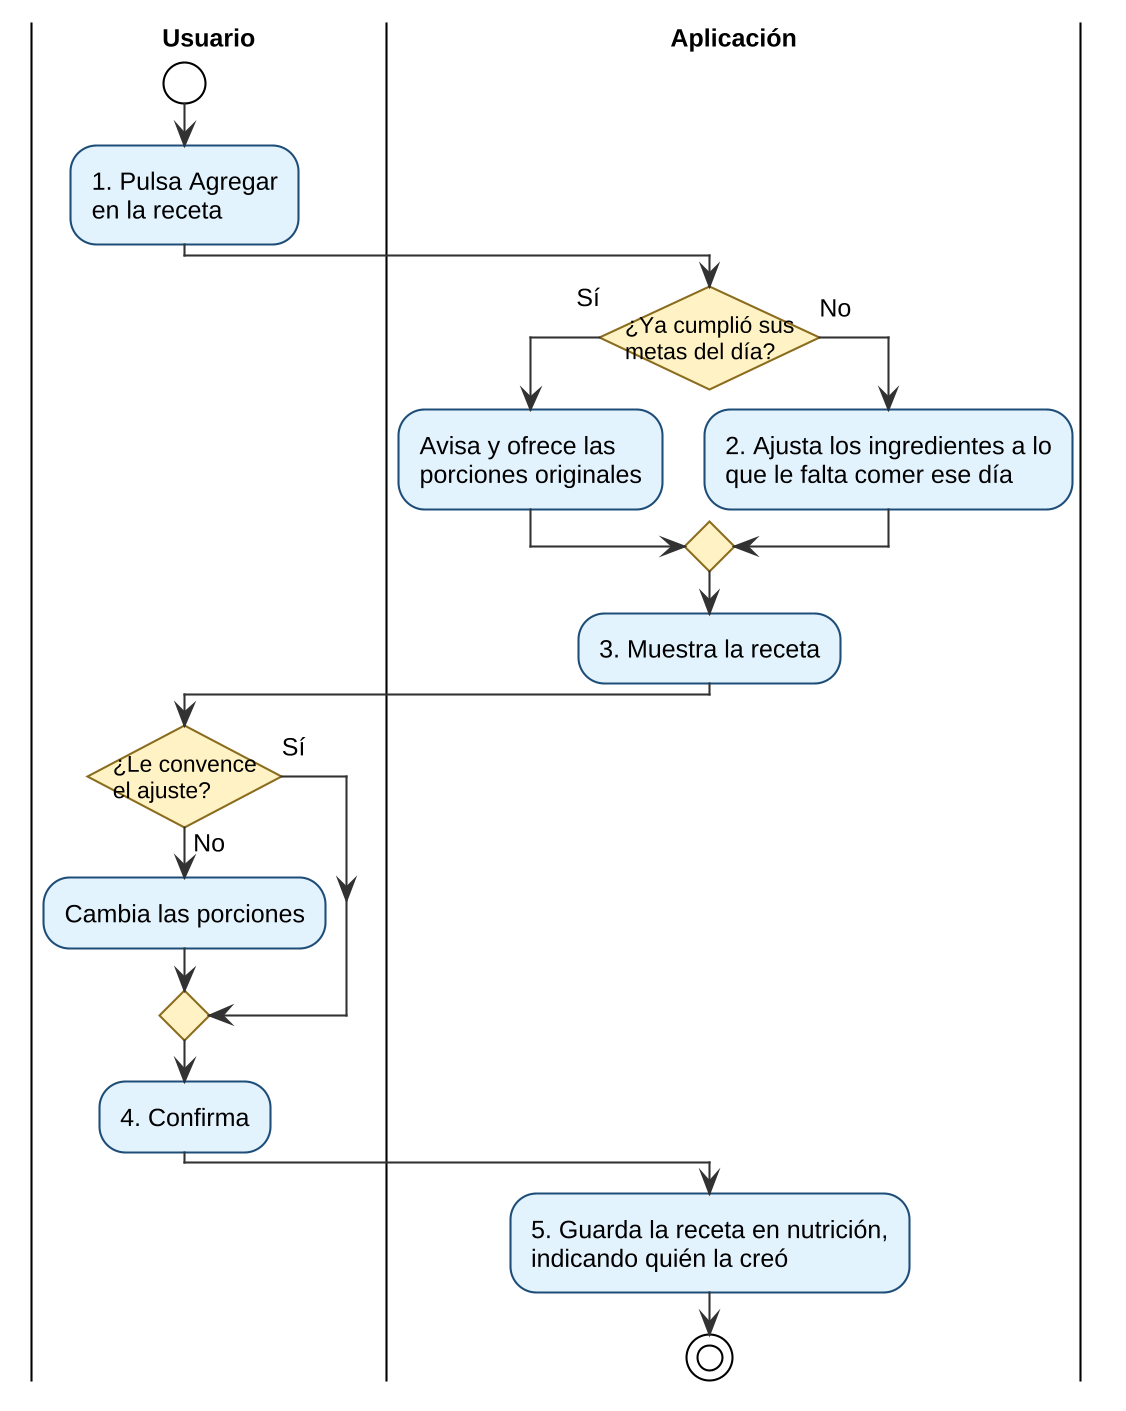
\includegraphics[width=0.78\textwidth,height=0.42\textheight,keepaspectratio]{figuras/diseno/dga_cu08.png}
    \captionof{figure}{Diagrama de Actividades -- CU-08: Agregar una receta ajustada a mis metas.}
    \label{fig:dga_cu08}
\end{center}

\noindent\begin{minipage}{\linewidth}
\textbf{Descripción Esencial Expandida del Caso de Uso}
\par\vspace{0.2cm}
\noindent
{\renewcommand{\arraystretch}{1.25}\setstretch{1}\small
\begin{tabular}{|>{\raggedright\arraybackslash}p{2.9cm}|>{\raggedright\arraybackslash}p{12.1cm}|}
    \hline
    \rowcolor[HTML]{EFEFEF} \textbf{Propósito} & Llevar una receta de otra persona al módulo de nutrición, con porciones adaptadas a lo que el atleta necesita ese día. \\ \hline
    \textbf{Tipo} & Primario \\ \hline
    \textbf{Actores} & Atleta Híbrido \\ \hline
    \textbf{Requerimientos} & R12 \\ \hline
    \textbf{Precondiciones} & El usuario inició sesión y tiene el plan premium. Ve una receta en su muro. \\ \hline
    \textbf{Poscondiciones} & La receta queda en el módulo de nutrición. No se registra como comida hasta que el atleta la anote en su diario. \\ \hline
\end{tabular}

\vspace{0.15cm}
\noindent
\begin{tabular}{|>{\raggedright\arraybackslash}p{7.5cm}|>{\raggedright\arraybackslash}p{7.5cm}|}
    \hline
    \rowcolor[HTML]{D9E1F2} \multicolumn{2}{|c|}{\textbf{Curso Normal de los Eventos}} \\ \hline
    \rowcolor[HTML]{EFEFEF} \multicolumn{1}{|c|}{\textbf{Usuario}} & \multicolumn{1}{c|}{\textbf{Respuesta del Sistema}} \\ \hline
        1. Pulsa Agregar en la receta. & 2. Revisa lo que le falta comer ese día y ajusta la cantidad de cada ingrediente, manteniendo las proporciones. \\ \hline
         & 3. Muestra la receta ajustada. \\ \hline
        4. Confirma. & 5. Guarda la receta en su módulo de nutrición, indicando quién la creó. \\ \hline
    \rowcolor[HTML]{F2D9D9} \multicolumn{2}{|c|}{\textbf{Cursos Alternos}} \\ \hline
    \rowcolor[HTML]{EFEFEF} \multicolumn{1}{|c|}{\textbf{Usuario}} & \multicolumn{1}{c|}{\textbf{Respuesta del Sistema}} \\ \hline
         & 2. Si ya cumplió sus metas del día, avisa y ofrece guardar la receta con sus porciones originales. \\ \hline
        4. Si no le convence el ajuste, puede cambiar las porciones antes de confirmar. &  \\ \hline
\end{tabular}
}
\end{minipage}
\vspace{0.4cm}

\subsubsection{CU-09. Publicar una sesión, ruta o comida}

\textbf{Diagrama de Actividades}
\begin{center}
    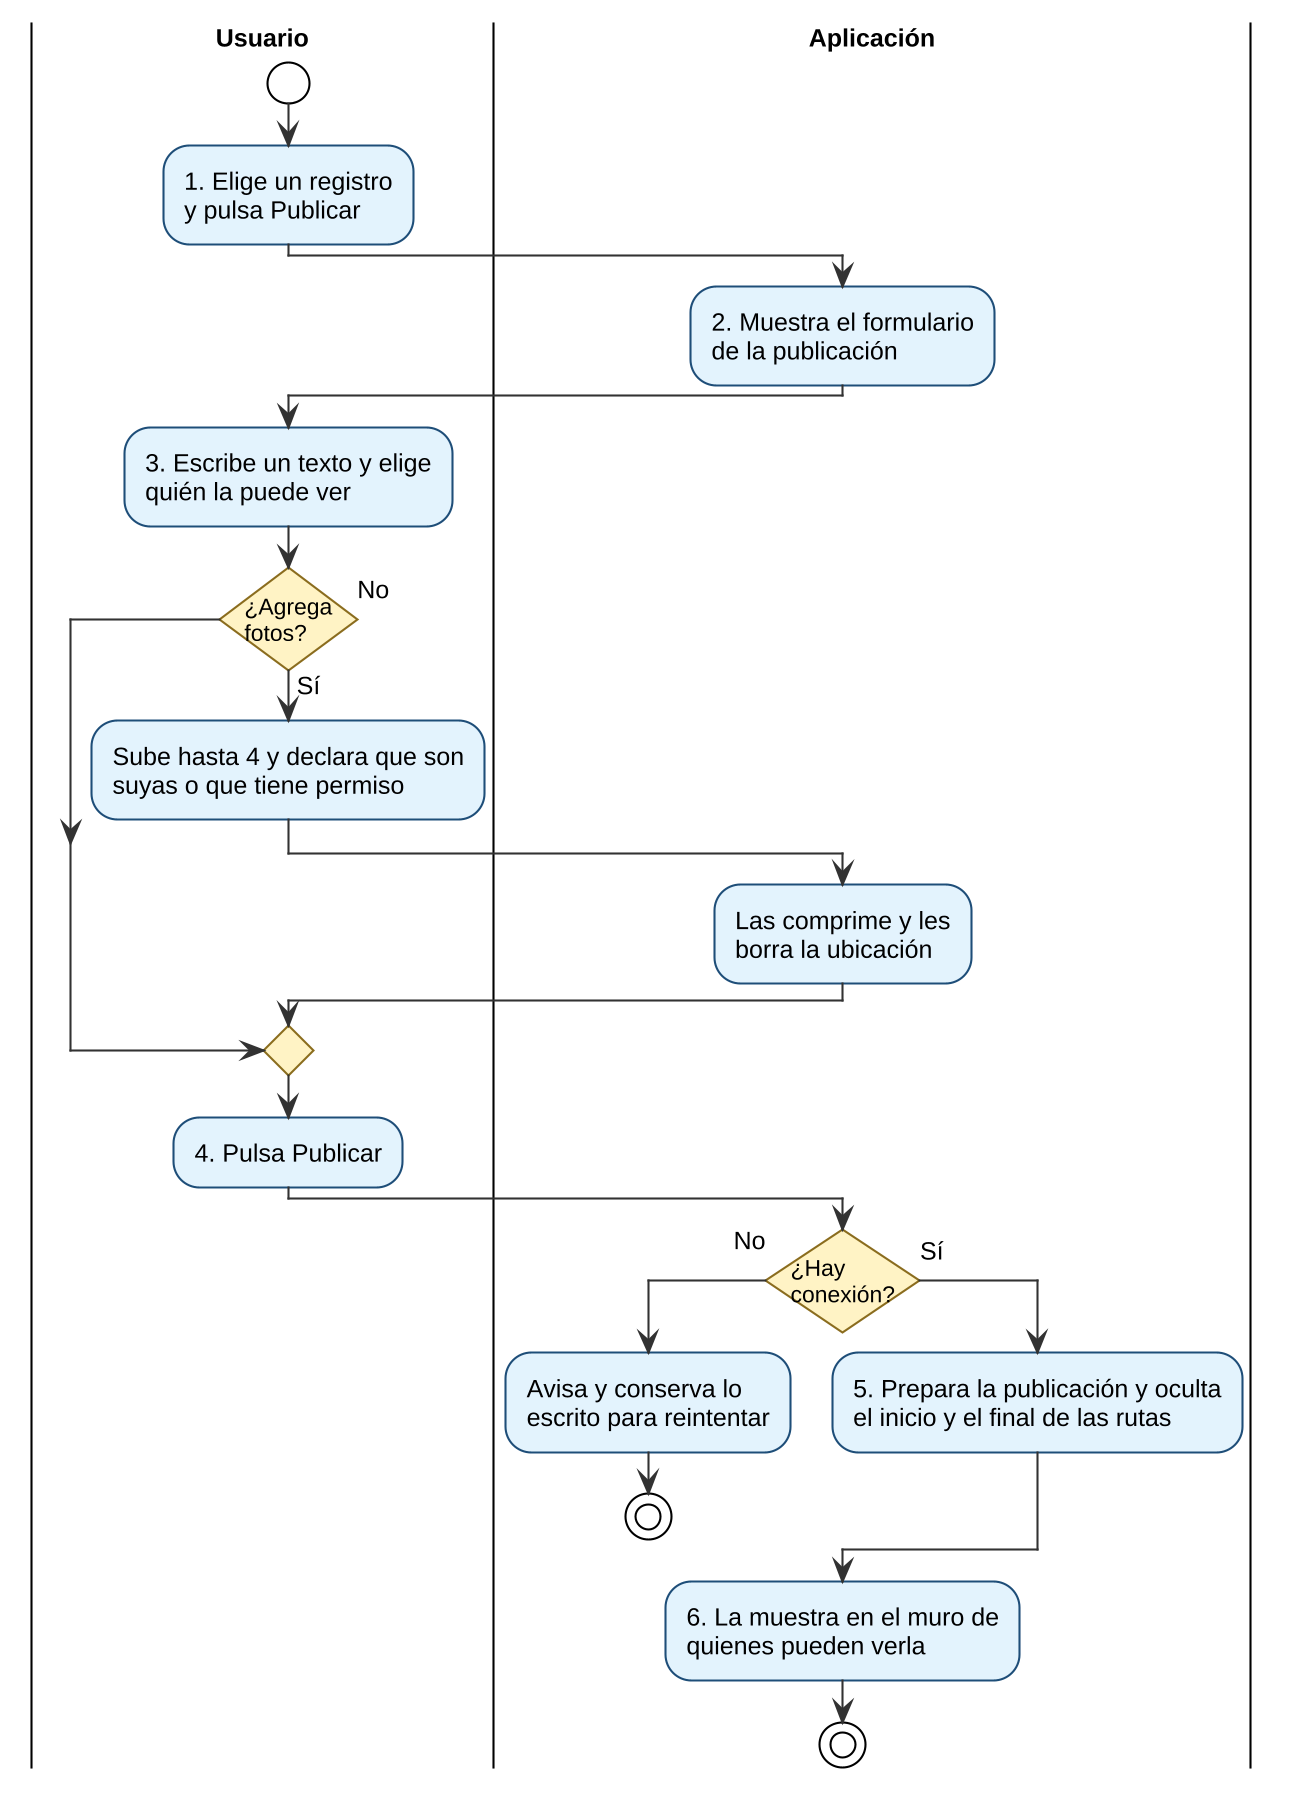
\includegraphics[width=0.78\textwidth,height=0.42\textheight,keepaspectratio]{figuras/diseno/dga_cu09.png}
    \captionof{figure}{Diagrama de Actividades -- CU-09: Publicar una sesión, ruta o comida.}
    \label{fig:dga_cu09}
\end{center}

\noindent\begin{minipage}{\linewidth}
\textbf{Descripción Esencial Expandida del Caso de Uso}
\par\vspace{0.2cm}
\noindent
{\renewcommand{\arraystretch}{1.25}\setstretch{1}\small
\begin{tabular}{|>{\raggedright\arraybackslash}p{2.9cm}|>{\raggedright\arraybackslash}p{12.1cm}|}
    \hline
    \rowcolor[HTML]{EFEFEF} \textbf{Propósito} & Compartir con la comunidad algo que el atleta ya registró o creó, como una receta propia (CU-27). \\ \hline
    \textbf{Tipo} & Primario \\ \hline
    \textbf{Actores} & Atleta Híbrido \\ \hline
    \textbf{Requerimientos} & R08, R15 \\ \hline
    \textbf{Precondiciones} & El usuario inició sesión y tiene el plan premium. Tiene al menos un registro guardado. \\ \hline
    \textbf{Poscondiciones} & La publicación queda visible solo para quienes el atleta eligió. \\ \hline
\end{tabular}

\vspace{0.15cm}
\noindent
\begin{tabular}{|>{\raggedright\arraybackslash}p{7.5cm}|>{\raggedright\arraybackslash}p{7.5cm}|}
    \hline
    \rowcolor[HTML]{D9E1F2} \multicolumn{2}{|c|}{\textbf{Curso Normal de los Eventos}} \\ \hline
    \rowcolor[HTML]{EFEFEF} \multicolumn{1}{|c|}{\textbf{Usuario}} & \multicolumn{1}{c|}{\textbf{Respuesta del Sistema}} \\ \hline
        1. Elige un registro (una sesión, una ruta, una comida o una receta) y pulsa Publicar. & 2. Muestra el formulario de la publicación. \\ \hline
        3. Escribe un texto y elige quién la puede ver (todos, sus seguidores o solo él). &  \\ \hline
        4. Pulsa Publicar. & 5. Prepara la publicación. Si es una ruta, oculta el inicio y el final del recorrido. \\ \hline
         & 6. Muestra la publicación en el muro de quienes pueden verla. \\ \hline
    \rowcolor[HTML]{F2D9D9} \multicolumn{2}{|c|}{\textbf{Cursos Alternos}} \\ \hline
    \rowcolor[HTML]{EFEFEF} \multicolumn{1}{|c|}{\textbf{Usuario}} & \multicolumn{1}{c|}{\textbf{Respuesta del Sistema}} \\ \hline
        3. Si agrega fotos, puede subir hasta 4 y declara que son suyas o que tiene permiso. La aplicación las comprime y les borra la ubicación. &  \\ \hline
        3. Si intenta agregar más de 4 fotos, la aplicación no lo permite y le avisa. &  \\ \hline
         & 5. Si se corta la conexión, avisa que no se pudo publicar y conserva lo escrito para reintentar. \\ \hline
\end{tabular}
}
\end{minipage}
\vspace{0.4cm}

\subsubsection{CU-10. Mantener el catálogo de ejercicios}

\textbf{Diagrama de Actividades}
\begin{center}
    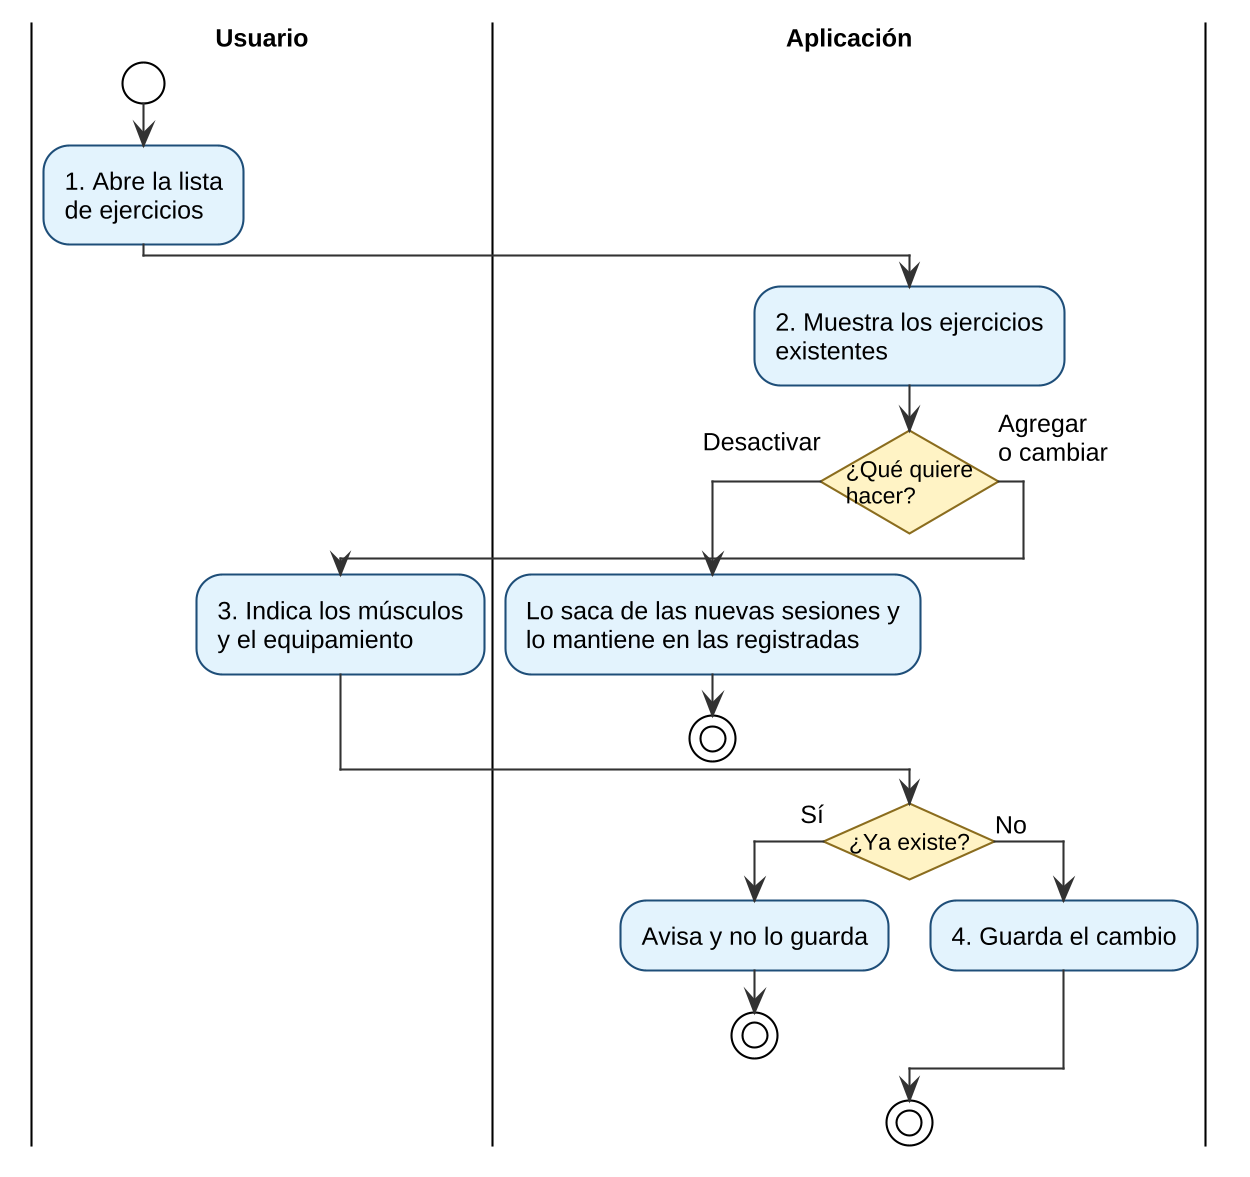
\includegraphics[width=0.78\textwidth,height=0.42\textheight,keepaspectratio]{figuras/diseno/dga_cu10.png}
    \captionof{figure}{Diagrama de Actividades -- CU-10: Mantener el catálogo de ejercicios.}
    \label{fig:dga_cu10}
\end{center}

\noindent\begin{minipage}{\linewidth}
\textbf{Descripción Esencial Expandida del Caso de Uso}
\par\vspace{0.2cm}
\noindent
{\renewcommand{\arraystretch}{1.25}\setstretch{1}\small
\begin{tabular}{|>{\raggedright\arraybackslash}p{2.9cm}|>{\raggedright\arraybackslash}p{12.1cm}|}
    \hline
    \rowcolor[HTML]{EFEFEF} \textbf{Propósito} & Mantener al día la lista de ejercicios que usan los atletas. \\ \hline
    \textbf{Tipo} & Primario \\ \hline
    \textbf{Actores} & Administrador \\ \hline
    \textbf{Requerimientos} & R11 \\ \hline
    \textbf{Precondiciones} & El administrador inició sesión en el panel de administración. \\ \hline
    \textbf{Poscondiciones} & La lista de ejercicios queda actualizada para todos los atletas. \\ \hline
\end{tabular}

\vspace{0.15cm}
\noindent
\begin{tabular}{|>{\raggedright\arraybackslash}p{7.5cm}|>{\raggedright\arraybackslash}p{7.5cm}|}
    \hline
    \rowcolor[HTML]{D9E1F2} \multicolumn{2}{|c|}{\textbf{Curso Normal de los Eventos}} \\ \hline
    \rowcolor[HTML]{EFEFEF} \multicolumn{1}{|c|}{\textbf{Usuario}} & \multicolumn{1}{c|}{\textbf{Respuesta del Sistema}} \\ \hline
        1. Abre la lista de ejercicios. & 2. Muestra los ejercicios existentes. \\ \hline
        3. Agrega o cambia un ejercicio, indicando qué músculos trabaja y qué equipamiento necesita. & 4. Revisa que no esté repetido y guarda el cambio. \\ \hline
    \rowcolor[HTML]{F2D9D9} \multicolumn{2}{|c|}{\textbf{Cursos Alternos}} \\ \hline
    \rowcolor[HTML]{EFEFEF} \multicolumn{1}{|c|}{\textbf{Usuario}} & \multicolumn{1}{c|}{\textbf{Respuesta del Sistema}} \\ \hline
        3. Si desactiva un ejercicio, este deja de aparecer para nuevas sesiones, pero se mantiene en las ya registradas. &  \\ \hline
         & 4. Si el ejercicio ya existe, avisa y no lo guarda. \\ \hline
\end{tabular}
}
\end{minipage}
\vspace{0.4cm}

\subsubsection{CU-11. Revisar el contenido reportado}

\textbf{Diagrama de Actividades}
\begin{center}
    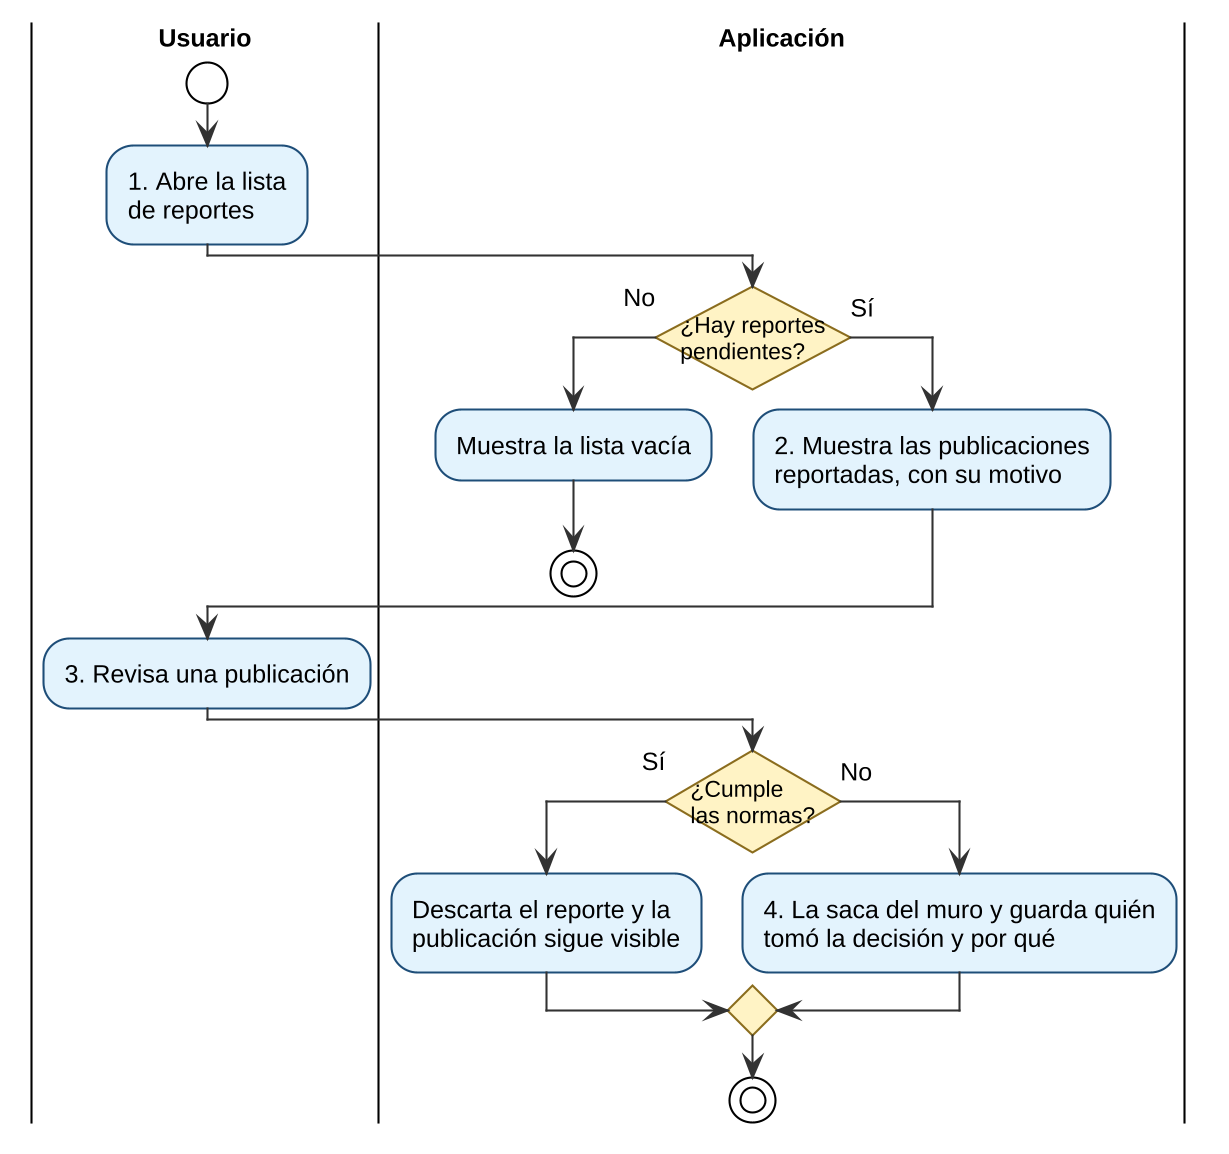
\includegraphics[width=0.78\textwidth,height=0.42\textheight,keepaspectratio]{figuras/diseno/dga_cu11.png}
    \captionof{figure}{Diagrama de Actividades -- CU-11: Revisar el contenido reportado.}
    \label{fig:dga_cu11}
\end{center}

\noindent\begin{minipage}{\linewidth}
\textbf{Descripción Esencial Expandida del Caso de Uso}
\par\vspace{0.2cm}
\noindent
{\renewcommand{\arraystretch}{1.25}\setstretch{1}\small
\begin{tabular}{|>{\raggedright\arraybackslash}p{2.9cm}|>{\raggedright\arraybackslash}p{12.1cm}|}
    \hline
    \rowcolor[HTML]{EFEFEF} \textbf{Propósito} & Retirar de la comunidad lo que no cumpla las normas o pueda ser peligroso para la salud. \\ \hline
    \textbf{Tipo} & Primario \\ \hline
    \textbf{Actores} & Administrador \\ \hline
    \textbf{Requerimientos} & R11 \\ \hline
    \textbf{Precondiciones} & El administrador inició sesión en el panel de administración. \\ \hline
    \textbf{Poscondiciones} & El reporte queda resuelto y hay registro de la decisión. \\ \hline
\end{tabular}

\vspace{0.15cm}
\noindent
\begin{tabular}{|>{\raggedright\arraybackslash}p{7.5cm}|>{\raggedright\arraybackslash}p{7.5cm}|}
    \hline
    \rowcolor[HTML]{D9E1F2} \multicolumn{2}{|c|}{\textbf{Curso Normal de los Eventos}} \\ \hline
    \rowcolor[HTML]{EFEFEF} \multicolumn{1}{|c|}{\textbf{Usuario}} & \multicolumn{1}{c|}{\textbf{Respuesta del Sistema}} \\ \hline
        1. Abre la lista de reportes. & 2. Muestra las publicaciones reportadas, con su motivo. \\ \hline
        3. Revisa una publicación y decide ocultarla. & 4. La saca del muro y guarda quién tomó la decisión y por qué. \\ \hline
    \rowcolor[HTML]{F2D9D9} \multicolumn{2}{|c|}{\textbf{Cursos Alternos}} \\ \hline
    \rowcolor[HTML]{EFEFEF} \multicolumn{1}{|c|}{\textbf{Usuario}} & \multicolumn{1}{c|}{\textbf{Respuesta del Sistema}} \\ \hline
         & 2. Si no hay reportes pendientes, muestra la lista vacía. \\ \hline
        3. Si la publicación cumple las normas, descarta el reporte y la publicación sigue visible. &  \\ \hline
\end{tabular}
}
\end{minipage}
\vspace{0.4cm}

\subsubsection{CU-12. Completar mi perfil y recibir un plan semanal}

\textbf{Diagrama de Actividades}
\begin{center}
    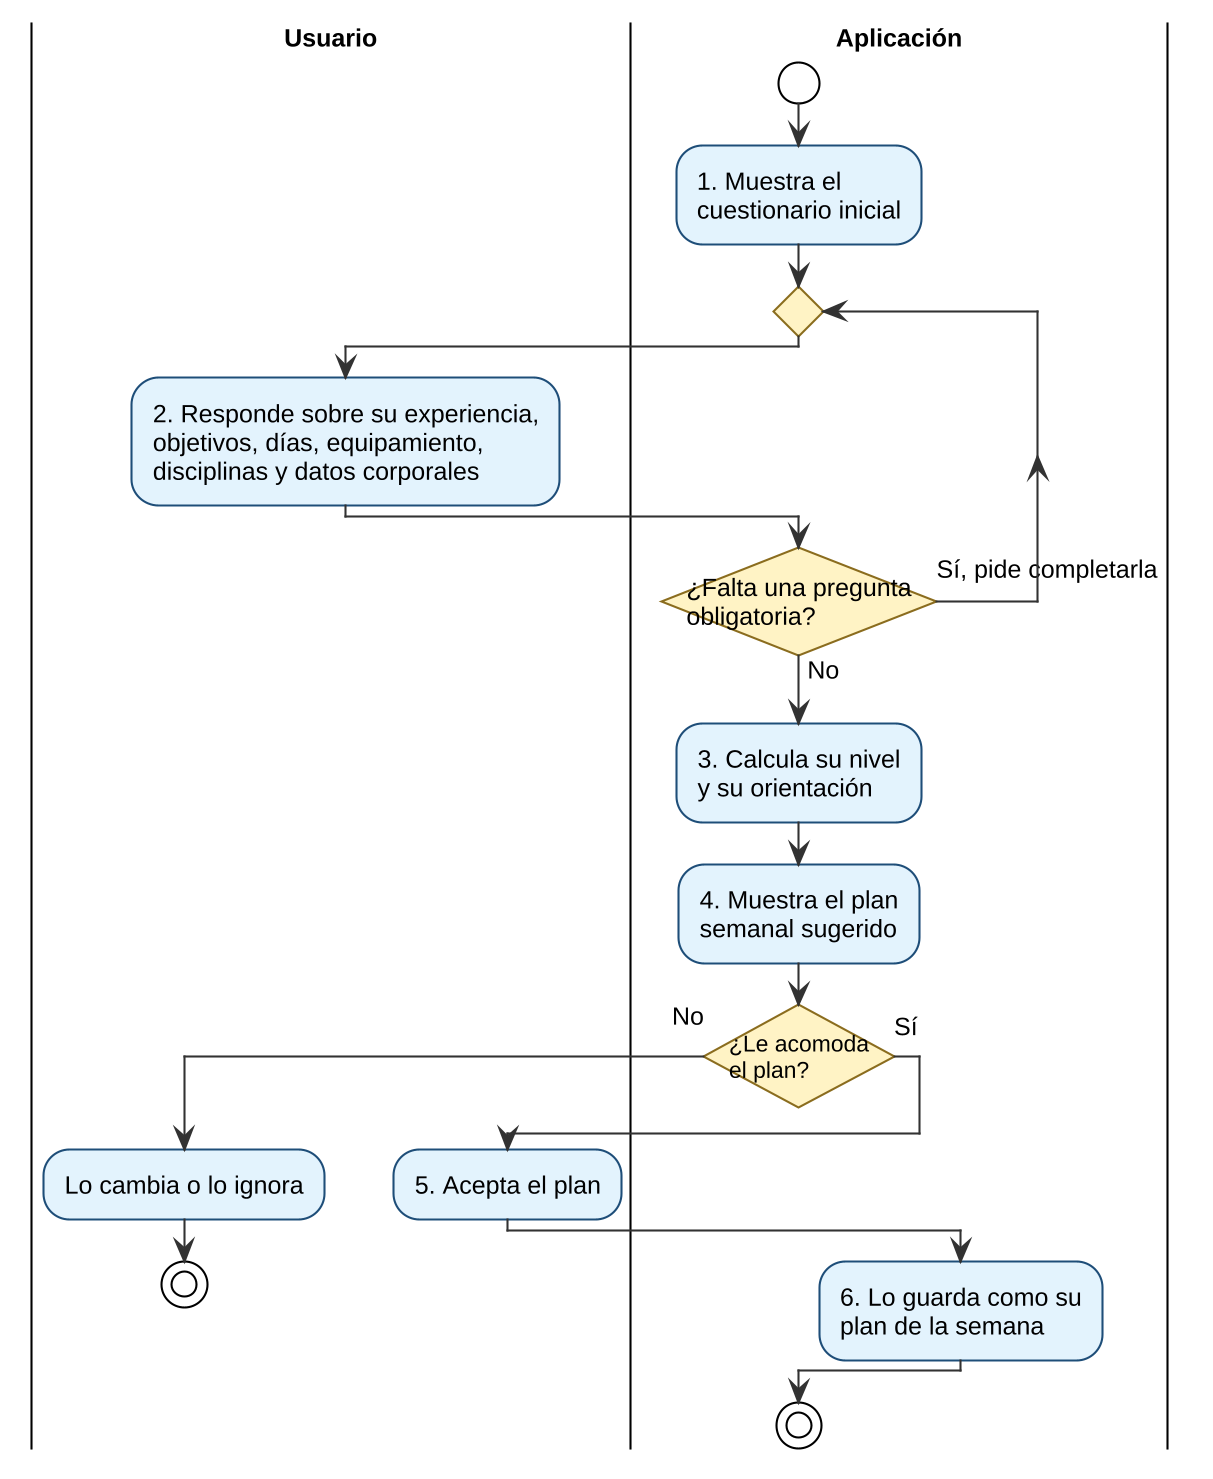
\includegraphics[width=0.78\textwidth,height=0.42\textheight,keepaspectratio]{figuras/diseno/dga_cu12.png}
    \captionof{figure}{Diagrama de Actividades -- CU-12: Completar mi perfil y recibir un plan semanal.}
    \label{fig:dga_cu12}
\end{center}

\noindent\begin{minipage}{\linewidth}
\textbf{Descripción Esencial Expandida del Caso de Uso}
\par\vspace{0.2cm}
\noindent
{\renewcommand{\arraystretch}{1.25}\setstretch{1}\small
\begin{tabular}{|>{\raggedright\arraybackslash}p{2.9cm}|>{\raggedright\arraybackslash}p{12.1cm}|}
    \hline
    \rowcolor[HTML]{EFEFEF} \textbf{Propósito} & Conocer al atleta para sugerirle un plan de entrenamiento según su nivel y sus objetivos. \\ \hline
    \textbf{Tipo} & Primario \\ \hline
    \textbf{Actores} & Atleta Básico, Atleta Híbrido \\ \hline
    \textbf{Requerimientos} & R13 \\ \hline
    \textbf{Precondiciones} & El usuario creó su cuenta y aceptó los términos de uso (CU-26). \\ \hline
    \textbf{Poscondiciones} & El perfil queda completo y el atleta tiene un plan sugerido para la semana. \\ \hline
\end{tabular}

\vspace{0.15cm}
\noindent
\begin{tabular}{|>{\raggedright\arraybackslash}p{7.5cm}|>{\raggedright\arraybackslash}p{7.5cm}|}
    \hline
    \rowcolor[HTML]{D9E1F2} \multicolumn{2}{|c|}{\textbf{Curso Normal de los Eventos}} \\ \hline
    \rowcolor[HTML]{EFEFEF} \multicolumn{1}{|c|}{\textbf{Usuario}} & \multicolumn{1}{c|}{\textbf{Respuesta del Sistema}} \\ \hline
         & 1. Muestra el cuestionario inicial. \\ \hline
        2. Responde sobre su experiencia, sus objetivos, los días que puede entrenar, su equipamiento, sus disciplinas, su edad, su sexo, su estatura y su peso. & 3. Calcula su nivel y su orientación. \\ \hline
         & 4. Muestra el plan semanal sugerido. \\ \hline
        5. Acepta el plan. & 6. Lo guarda como su plan de la semana. \\ \hline
    \rowcolor[HTML]{F2D9D9} \multicolumn{2}{|c|}{\textbf{Cursos Alternos}} \\ \hline
    \rowcolor[HTML]{EFEFEF} \multicolumn{1}{|c|}{\textbf{Usuario}} & \multicolumn{1}{c|}{\textbf{Respuesta del Sistema}} \\ \hline
        2. Si deja una pregunta obligatoria sin responder, la aplicación le pide completarla. &  \\ \hline
        5. Si no le acomoda, puede cambiar el plan o ignorarlo. La aplicación sigue funcionando igual. &  \\ \hline
\end{tabular}
}
\end{minipage}
\vspace{0.4cm}

\subsubsection{CU-13. Agregar una publicación a mis módulos}

\textbf{Diagrama de Actividades}
\begin{center}
    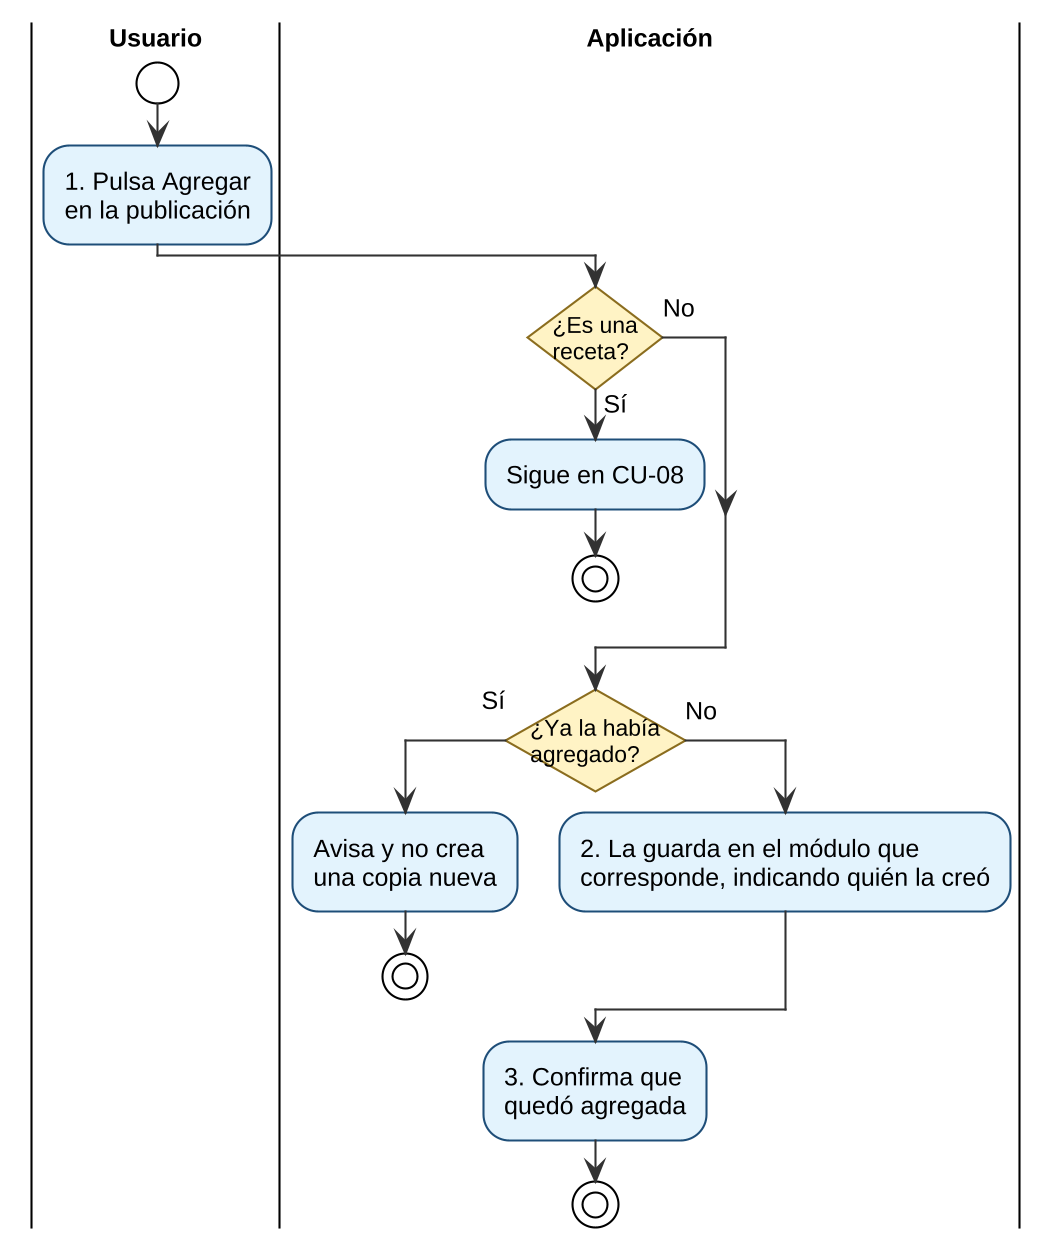
\includegraphics[width=0.78\textwidth,height=0.42\textheight,keepaspectratio]{figuras/diseno/dga_cu13.png}
    \captionof{figure}{Diagrama de Actividades -- CU-13: Agregar una publicación a mis módulos.}
    \label{fig:dga_cu13}
\end{center}

\noindent\begin{minipage}{\linewidth}
\textbf{Descripción Esencial Expandida del Caso de Uso}
\par\vspace{0.2cm}
\noindent
{\renewcommand{\arraystretch}{1.25}\setstretch{1}\small
\begin{tabular}{|>{\raggedright\arraybackslash}p{2.9cm}|>{\raggedright\arraybackslash}p{12.1cm}|}
    \hline
    \rowcolor[HTML]{EFEFEF} \textbf{Propósito} & Usar lo que publicó otra persona sin tener que copiarlo a mano. \\ \hline
    \textbf{Tipo} & Primario \\ \hline
    \textbf{Actores} & Atleta Híbrido \\ \hline
    \textbf{Requerimientos} & R12 \\ \hline
    \textbf{Precondiciones} & El usuario inició sesión y tiene el plan premium. Ve la publicación en su muro. \\ \hline
    \textbf{Poscondiciones} & El contenido queda disponible en los módulos del atleta. \\ \hline
\end{tabular}

\vspace{0.15cm}
\noindent
\begin{tabular}{|>{\raggedright\arraybackslash}p{7.5cm}|>{\raggedright\arraybackslash}p{7.5cm}|}
    \hline
    \rowcolor[HTML]{D9E1F2} \multicolumn{2}{|c|}{\textbf{Curso Normal de los Eventos}} \\ \hline
    \rowcolor[HTML]{EFEFEF} \multicolumn{1}{|c|}{\textbf{Usuario}} & \multicolumn{1}{c|}{\textbf{Respuesta del Sistema}} \\ \hline
        1. Pulsa Agregar en la publicación. & 2. La guarda en el módulo que corresponde, indicando quién la creó. Una sesión queda en sus rutinas y una ruta en su módulo de cardio. \\ \hline
         & 3. Confirma que quedó agregada. \\ \hline
    \rowcolor[HTML]{F2D9D9} \multicolumn{2}{|c|}{\textbf{Cursos Alternos}} \\ \hline
    \rowcolor[HTML]{EFEFEF} \multicolumn{1}{|c|}{\textbf{Usuario}} & \multicolumn{1}{c|}{\textbf{Respuesta del Sistema}} \\ \hline
         & 2. Si la publicación es una receta, sigue el caso de uso CU-08. \\ \hline
         & 2. Si ya la había agregado, avisa y no crea una copia nueva. \\ \hline
\end{tabular}
}
\end{minipage}
\vspace{0.4cm}

\subsubsection{CU-14. Seguir a otro usuario}

\textbf{Diagrama de Actividades}
\begin{center}
    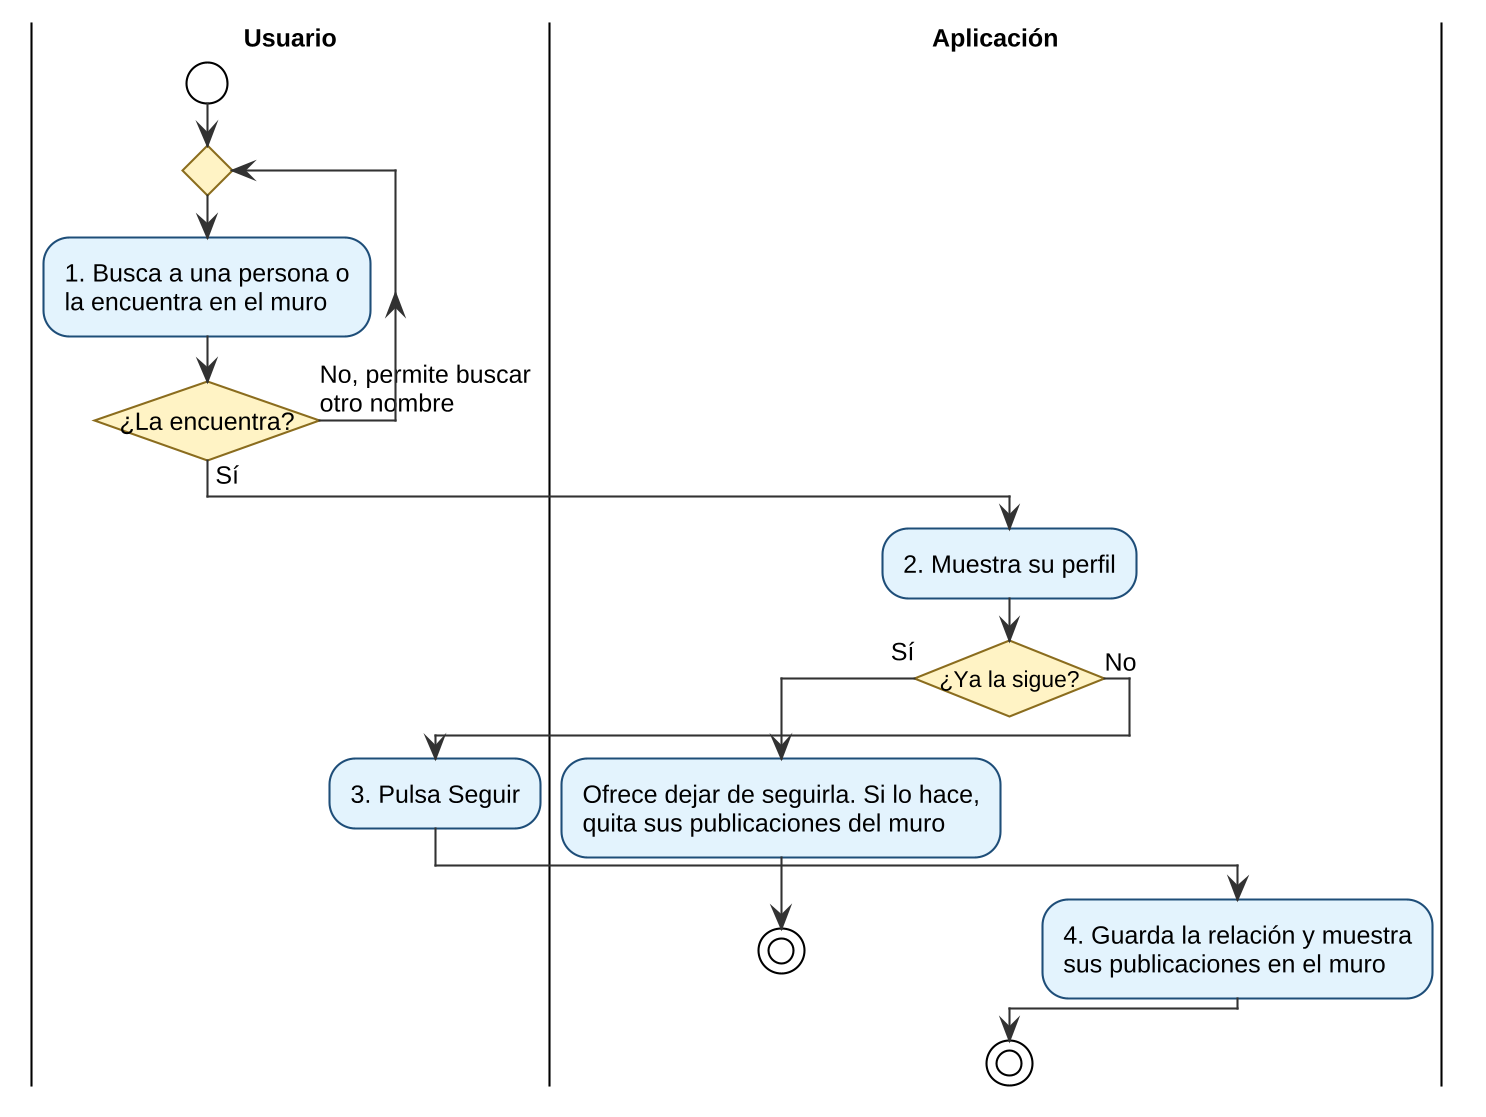
\includegraphics[width=0.78\textwidth,height=0.42\textheight,keepaspectratio]{figuras/diseno/dga_cu14.png}
    \captionof{figure}{Diagrama de Actividades -- CU-14: Seguir a otro usuario.}
    \label{fig:dga_cu14}
\end{center}

\noindent\begin{minipage}{\linewidth}
\textbf{Descripción Esencial Expandida del Caso de Uso}
\par\vspace{0.2cm}
\noindent
{\renewcommand{\arraystretch}{1.25}\setstretch{1}\small
\begin{tabular}{|>{\raggedright\arraybackslash}p{2.9cm}|>{\raggedright\arraybackslash}p{12.1cm}|}
    \hline
    \rowcolor[HTML]{EFEFEF} \textbf{Propósito} & Ver en el muro lo que publican otras personas. \\ \hline
    \textbf{Tipo} & Primario \\ \hline
    \textbf{Actores} & Atleta Híbrido \\ \hline
    \textbf{Requerimientos} & R08 \\ \hline
    \textbf{Precondiciones} & El usuario inició sesión y tiene el plan premium. \\ \hline
    \textbf{Poscondiciones} & El atleta sigue a esa persona y ve sus publicaciones. \\ \hline
\end{tabular}

\vspace{0.15cm}
\noindent
\begin{tabular}{|>{\raggedright\arraybackslash}p{7.5cm}|>{\raggedright\arraybackslash}p{7.5cm}|}
    \hline
    \rowcolor[HTML]{D9E1F2} \multicolumn{2}{|c|}{\textbf{Curso Normal de los Eventos}} \\ \hline
    \rowcolor[HTML]{EFEFEF} \multicolumn{1}{|c|}{\textbf{Usuario}} & \multicolumn{1}{c|}{\textbf{Respuesta del Sistema}} \\ \hline
        1. Busca a una persona o la encuentra en el muro. & 2. Muestra su perfil. \\ \hline
        3. Pulsa Seguir. & 4. Guarda la relación y desde ese momento muestra sus publicaciones en el muro. \\ \hline
    \rowcolor[HTML]{F2D9D9} \multicolumn{2}{|c|}{\textbf{Cursos Alternos}} \\ \hline
    \rowcolor[HTML]{EFEFEF} \multicolumn{1}{|c|}{\textbf{Usuario}} & \multicolumn{1}{c|}{\textbf{Respuesta del Sistema}} \\ \hline
         & 2. Si no encuentra a la persona, avisa y permite buscar otro nombre. \\ \hline
        3. Si ya la sigue, puede dejar de seguirla, y sus publicaciones ya no aparecen en el muro. &  \\ \hline
\end{tabular}
}
\end{minipage}
\vspace{0.4cm}

\subsubsection{CU-15. Registrar un producto con su código de barras}

\textbf{Diagrama de Actividades}
\begin{center}
    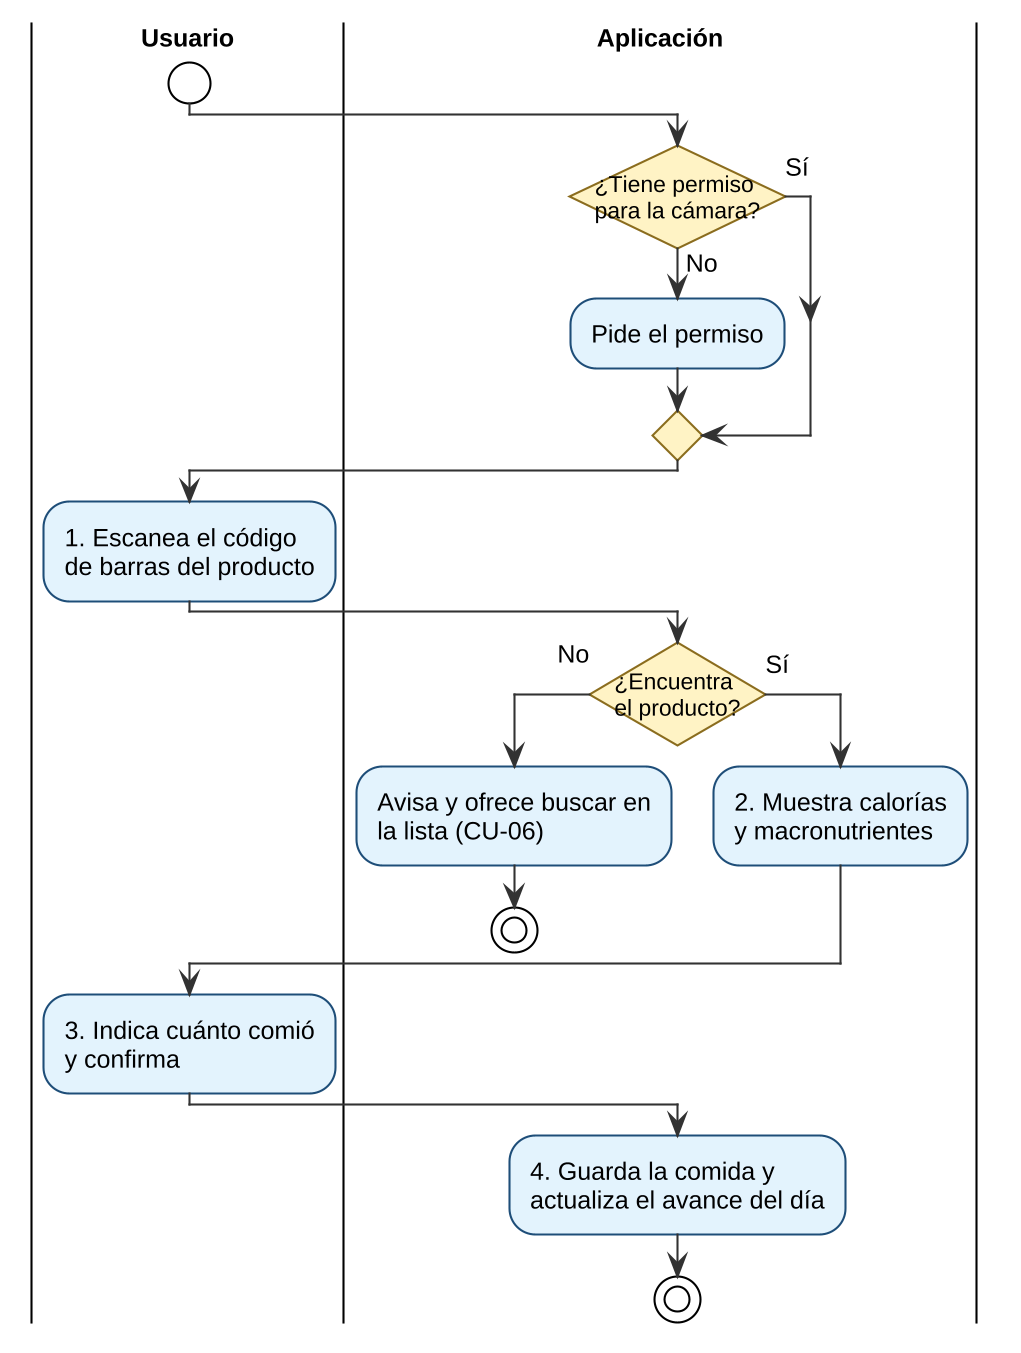
\includegraphics[width=0.78\textwidth,height=0.42\textheight,keepaspectratio]{figuras/diseno/dga_cu15.png}
    \captionof{figure}{Diagrama de Actividades -- CU-15: Registrar un producto con su código de barras.}
    \label{fig:dga_cu15}
\end{center}

\noindent\begin{minipage}{\linewidth}
\textbf{Descripción Esencial Expandida del Caso de Uso}
\par\vspace{0.2cm}
\noindent
{\renewcommand{\arraystretch}{1.25}\setstretch{1}\small
\begin{tabular}{|>{\raggedright\arraybackslash}p{2.9cm}|>{\raggedright\arraybackslash}p{12.1cm}|}
    \hline
    \rowcolor[HTML]{EFEFEF} \textbf{Propósito} & Registrar un producto envasado sin tener que buscarlo. \\ \hline
    \textbf{Tipo} & Primario \\ \hline
    \textbf{Actores} & Atleta Básico, Atleta Híbrido \\ \hline
    \textbf{Requerimientos} & R04 \\ \hline
    \textbf{Precondiciones} & El usuario inició sesión en la aplicación. \\ \hline
    \textbf{Poscondiciones} & La comida queda en el diario del día. \\ \hline
\end{tabular}

\vspace{0.15cm}
\noindent
\begin{tabular}{|>{\raggedright\arraybackslash}p{7.5cm}|>{\raggedright\arraybackslash}p{7.5cm}|}
    \hline
    \rowcolor[HTML]{D9E1F2} \multicolumn{2}{|c|}{\textbf{Curso Normal de los Eventos}} \\ \hline
    \rowcolor[HTML]{EFEFEF} \multicolumn{1}{|c|}{\textbf{Usuario}} & \multicolumn{1}{c|}{\textbf{Respuesta del Sistema}} \\ \hline
        1. Escanea con la cámara el código de barras del producto. & 2. Muestra el producto con sus calorías y sus macronutrientes. \\ \hline
        3. Indica cuánto comió y confirma. & 4. Guarda la comida en el diario y actualiza el avance del día. \\ \hline
    \rowcolor[HTML]{F2D9D9} \multicolumn{2}{|c|}{\textbf{Cursos Alternos}} \\ \hline
    \rowcolor[HTML]{EFEFEF} \multicolumn{1}{|c|}{\textbf{Usuario}} & \multicolumn{1}{c|}{\textbf{Respuesta del Sistema}} \\ \hline
        1. Si no ha dado permiso para usar la cámara, la aplicación se lo pide. &  \\ \hline
         & 2. Si no encuentra el producto, avisa y ofrece buscarlo en la lista de alimentos (CU-06). \\ \hline
\end{tabular}
}
\end{minipage}
\vspace{0.4cm}

\subsubsection{CU-16. Contar mi comida con mis palabras}

\textbf{Diagrama de Actividades}
\begin{center}
    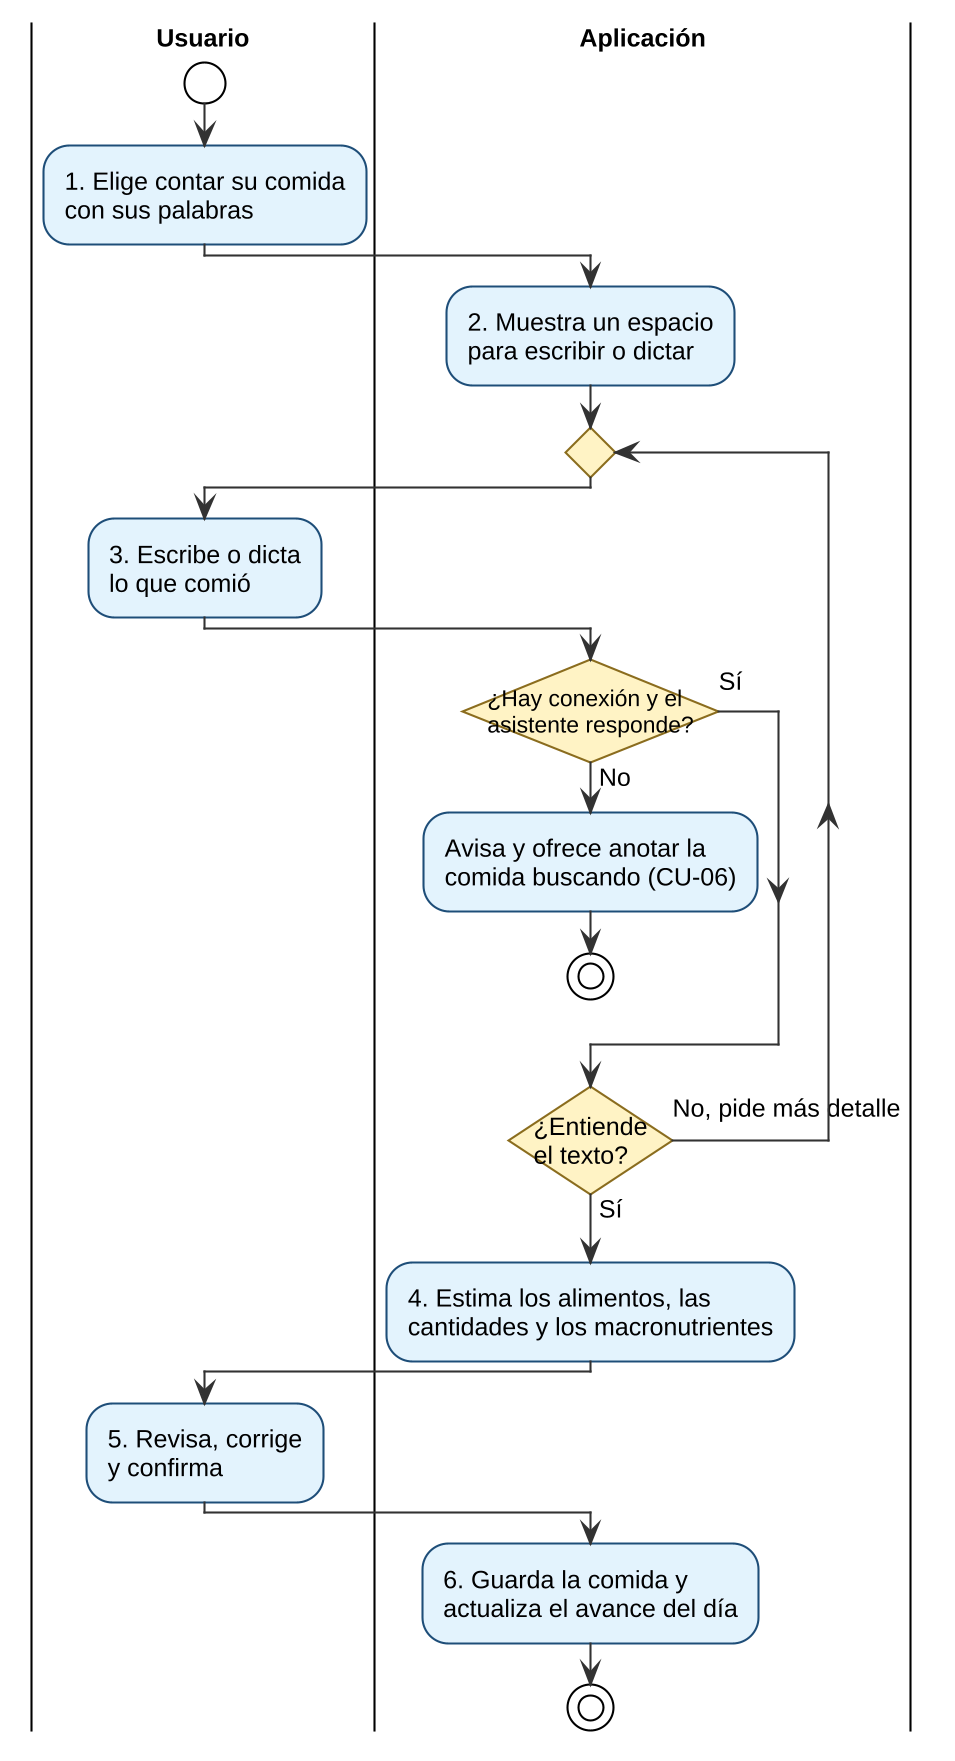
\includegraphics[width=0.78\textwidth,height=0.42\textheight,keepaspectratio]{figuras/diseno/dga_cu16.png}
    \captionof{figure}{Diagrama de Actividades -- CU-16: Contar mi comida con mis palabras.}
    \label{fig:dga_cu16}
\end{center}

\noindent\begin{minipage}{\linewidth}
\textbf{Descripción Esencial Expandida del Caso de Uso}
\par\vspace{0.2cm}
\noindent
{\renewcommand{\arraystretch}{1.25}\setstretch{1}\small
\begin{tabular}{|>{\raggedright\arraybackslash}p{2.9cm}|>{\raggedright\arraybackslash}p{12.1cm}|}
    \hline
    \rowcolor[HTML]{EFEFEF} \textbf{Propósito} & Registrar una comida escribiendo o dictando lo que se comió. \\ \hline
    \textbf{Tipo} & Primario \\ \hline
    \textbf{Actores} & Atleta Híbrido, Asistente de inteligencia artificial \\ \hline
    \textbf{Requerimientos} & R04 \\ \hline
    \textbf{Precondiciones} & El usuario inició sesión y tiene el plan premium. Tiene conexión a Internet. \\ \hline
    \textbf{Poscondiciones} & La comida confirmada queda en el diario del día. \\ \hline
\end{tabular}

\vspace{0.15cm}
\noindent
\begin{tabular}{|>{\raggedright\arraybackslash}p{7.5cm}|>{\raggedright\arraybackslash}p{7.5cm}|}
    \hline
    \rowcolor[HTML]{D9E1F2} \multicolumn{2}{|c|}{\textbf{Curso Normal de los Eventos}} \\ \hline
    \rowcolor[HTML]{EFEFEF} \multicolumn{1}{|c|}{\textbf{Usuario}} & \multicolumn{1}{c|}{\textbf{Respuesta del Sistema}} \\ \hline
        1. Elige contar su comida con sus palabras. & 2. Muestra un espacio para escribir o dictar. \\ \hline
        3. Escribe o dicta lo que comió, por ejemplo ``un plato de arroz con pollo y una ensalada''. & 4. Estima con ayuda del asistente de IA los alimentos, las cantidades y los macronutrientes. \\ \hline
        5. Revisa la estimación, corrige lo que haga falta y confirma. & 6. Guarda la comida en el diario y actualiza el avance del día. \\ \hline
    \rowcolor[HTML]{F2D9D9} \multicolumn{2}{|c|}{\textbf{Cursos Alternos}} \\ \hline
    \rowcolor[HTML]{EFEFEF} \multicolumn{1}{|c|}{\textbf{Usuario}} & \multicolumn{1}{c|}{\textbf{Respuesta del Sistema}} \\ \hline
         & 4. Si no logra entender el texto, pide al atleta que dé más detalle. \\ \hline
         & 4. Si no hay conexión o el asistente no responde, avisa y ofrece anotar la comida buscando los alimentos (CU-06). \\ \hline
\end{tabular}
}
\end{minipage}
\vspace{0.4cm}

\subsubsection{CU-17. Registrar una sesión de cardio sin reloj}

\textbf{Diagrama de Actividades}
\begin{center}
    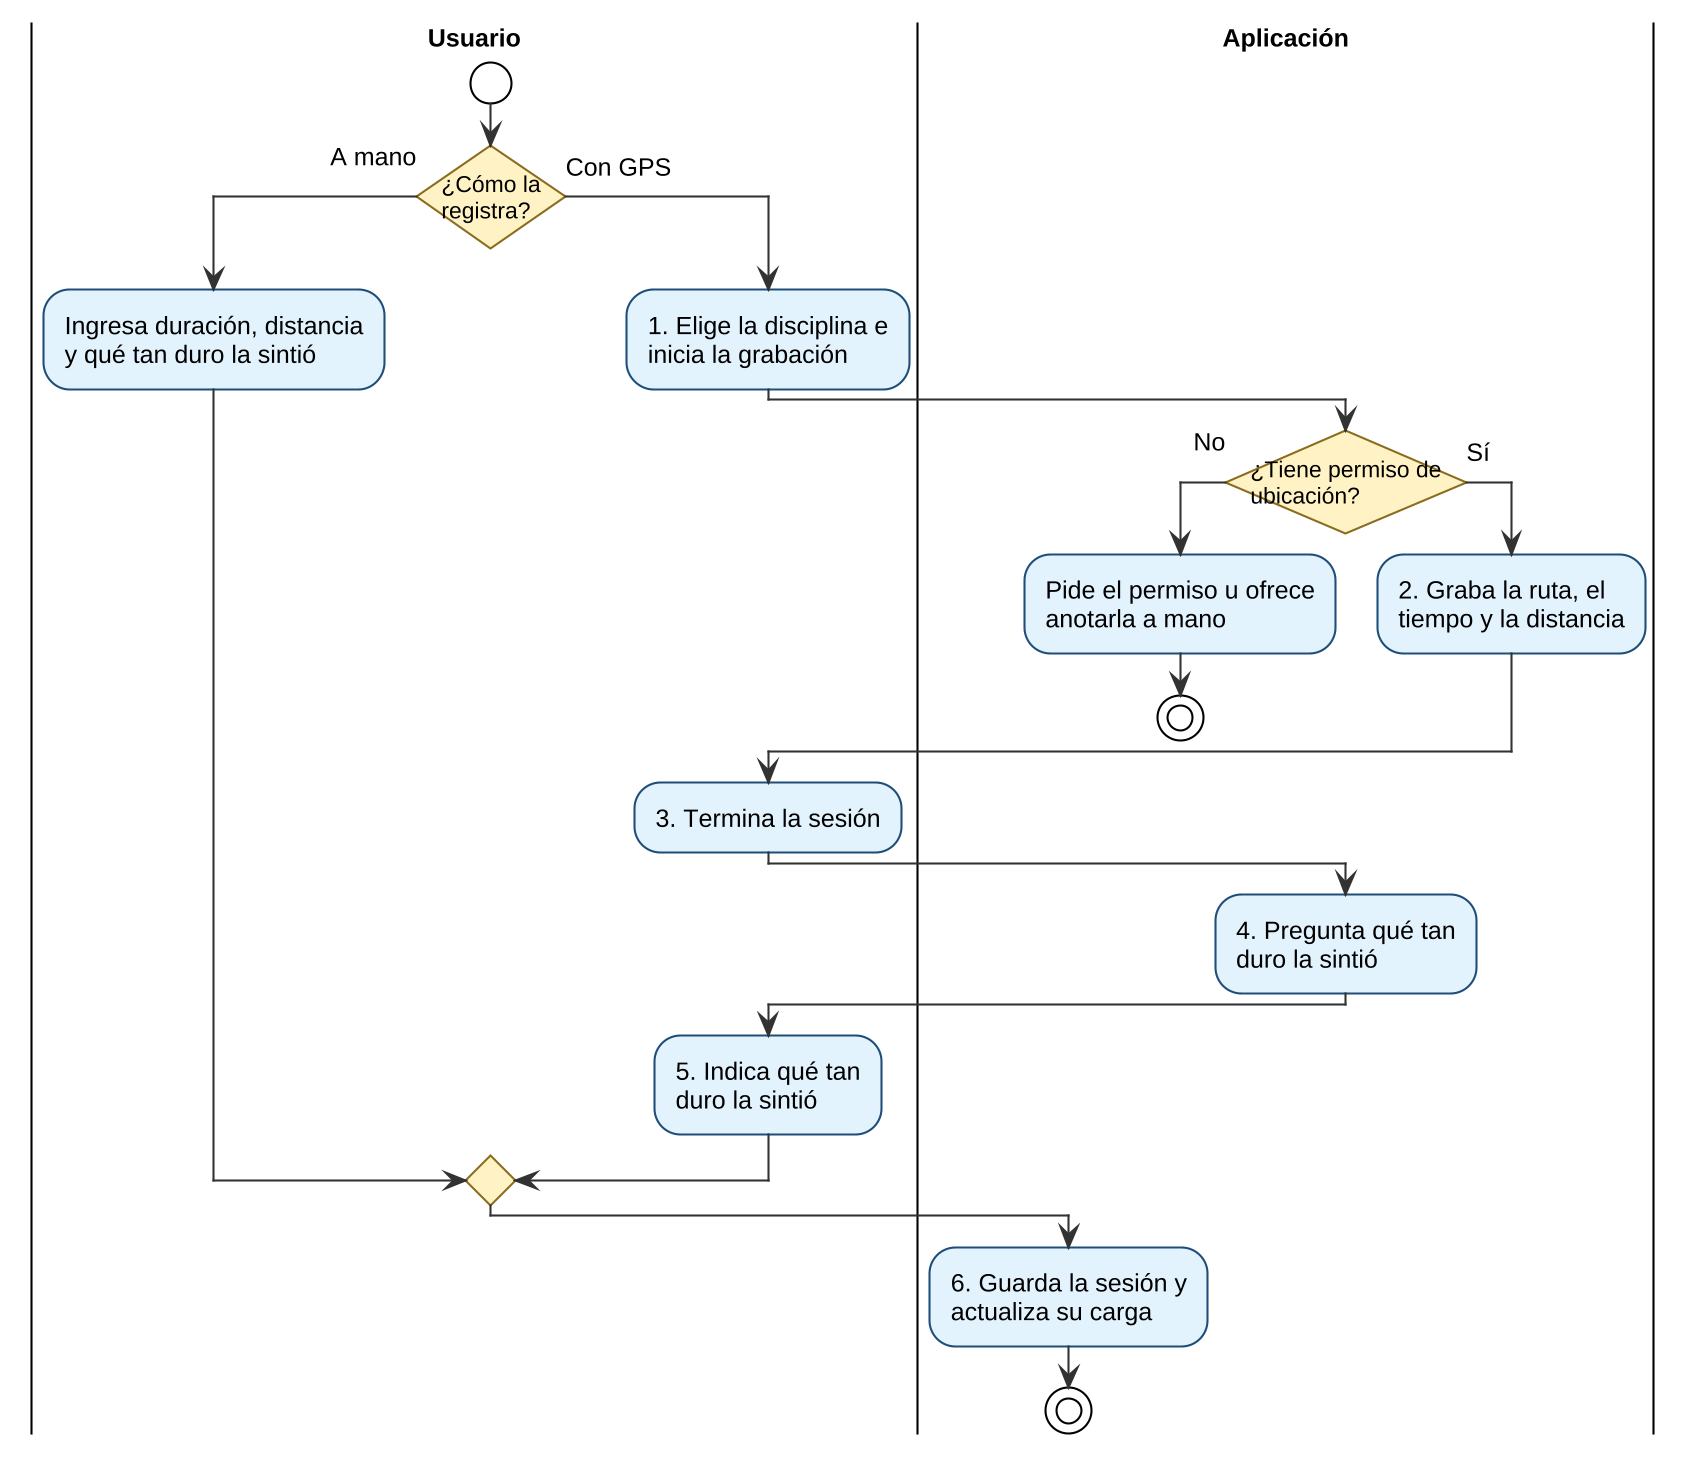
\includegraphics[width=0.78\textwidth,height=0.42\textheight,keepaspectratio]{figuras/diseno/dga_cu17.png}
    \captionof{figure}{Diagrama de Actividades -- CU-17: Registrar una sesión de cardio sin reloj.}
    \label{fig:dga_cu17}
\end{center}

\noindent\begin{minipage}{\linewidth}
\textbf{Descripción Esencial Expandida del Caso de Uso}
\par\vspace{0.2cm}
\noindent
{\renewcommand{\arraystretch}{1.25}\setstretch{1}\small
\begin{tabular}{|>{\raggedright\arraybackslash}p{2.9cm}|>{\raggedright\arraybackslash}p{12.1cm}|}
    \hline
    \rowcolor[HTML]{EFEFEF} \textbf{Propósito} & Registrar una salida de ciclismo, running o trekking usando solo el teléfono. \\ \hline
    \textbf{Tipo} & Primario \\ \hline
    \textbf{Actores} & Atleta Básico, Atleta Híbrido \\ \hline
    \textbf{Requerimientos} & R02 \\ \hline
    \textbf{Precondiciones} & El usuario inició sesión en la aplicación. \\ \hline
    \textbf{Poscondiciones} & La sesión queda en el historial del atleta y su carga queda actualizada. \\ \hline
\end{tabular}

\vspace{0.15cm}
\noindent
\begin{tabular}{|>{\raggedright\arraybackslash}p{7.5cm}|>{\raggedright\arraybackslash}p{7.5cm}|}
    \hline
    \rowcolor[HTML]{D9E1F2} \multicolumn{2}{|c|}{\textbf{Curso Normal de los Eventos}} \\ \hline
    \rowcolor[HTML]{EFEFEF} \multicolumn{1}{|c|}{\textbf{Usuario}} & \multicolumn{1}{c|}{\textbf{Respuesta del Sistema}} \\ \hline
        1. Elige la disciplina e inicia la grabación. & 2. Graba la ruta, el tiempo y la distancia con el GPS del teléfono. \\ \hline
        3. Termina la sesión. & 4. Pregunta qué tan duro la sintió. \\ \hline
        5. Indica qué tan duro la sintió. & 6. Guarda la sesión y actualiza su carga. \\ \hline
    \rowcolor[HTML]{F2D9D9} \multicolumn{2}{|c|}{\textbf{Cursos Alternos}} \\ \hline
    \rowcolor[HTML]{EFEFEF} \multicolumn{1}{|c|}{\textbf{Usuario}} & \multicolumn{1}{c|}{\textbf{Respuesta del Sistema}} \\ \hline
        1. Si prefiere anotarla a mano, ingresa la duración, la distancia y qué tan duro la sintió, y sigue en el paso 6. &  \\ \hline
         & 2. Si no tiene permiso para usar la ubicación, lo pide. Sin permiso, ofrece anotar la sesión a mano. \\ \hline
\end{tabular}
}
\end{minipage}
\vspace{0.4cm}

\subsubsection{CU-18. Ver mis metas de alimentación del día}

\textbf{Diagrama de Actividades}
\begin{center}
    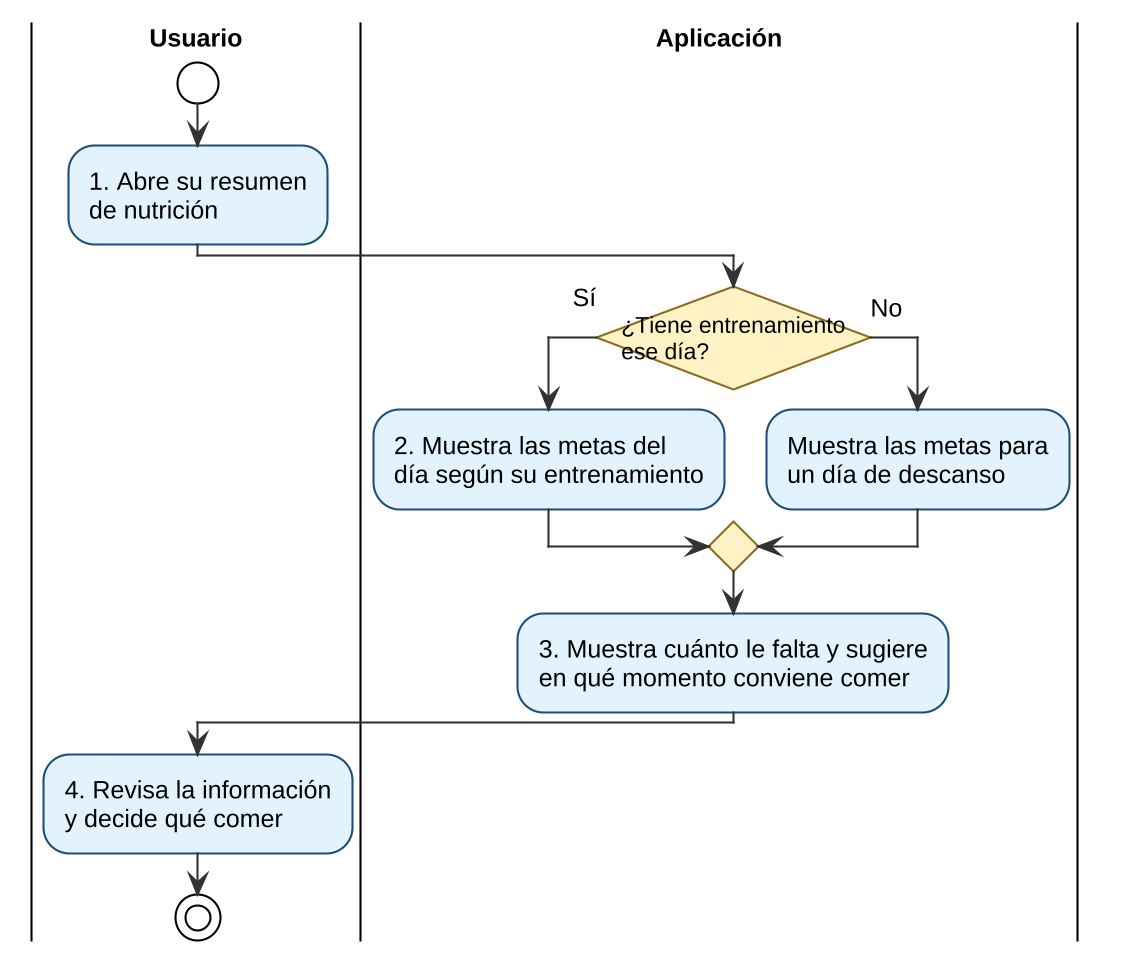
\includegraphics[width=0.78\textwidth,height=0.42\textheight,keepaspectratio]{figuras/diseno/dga_cu18.png}
    \captionof{figure}{Diagrama de Actividades -- CU-18: Ver mis metas de alimentación del día.}
    \label{fig:dga_cu18}
\end{center}

\noindent\begin{minipage}{\linewidth}
\textbf{Descripción Esencial Expandida del Caso de Uso}
\par\vspace{0.2cm}
\noindent
{\renewcommand{\arraystretch}{1.25}\setstretch{1}\small
\begin{tabular}{|>{\raggedright\arraybackslash}p{2.9cm}|>{\raggedright\arraybackslash}p{12.1cm}|}
    \hline
    \rowcolor[HTML]{EFEFEF} \textbf{Propósito} & Mostrar cuánto le conviene comer al atleta según lo que entrenó o tiene planificado. \\ \hline
    \textbf{Tipo} & Primario \\ \hline
    \textbf{Actores} & Atleta Híbrido \\ \hline
    \textbf{Requerimientos} & R05 \\ \hline
    \textbf{Precondiciones} & El usuario inició sesión y tiene el plan premium. Completó su perfil. \\ \hline
    \textbf{Poscondiciones} & El atleta conoce sus metas del día. Son sugerencias y no una dieta. \\ \hline
\end{tabular}

\vspace{0.15cm}
\noindent
\begin{tabular}{|>{\raggedright\arraybackslash}p{7.5cm}|>{\raggedright\arraybackslash}p{7.5cm}|}
    \hline
    \rowcolor[HTML]{D9E1F2} \multicolumn{2}{|c|}{\textbf{Curso Normal de los Eventos}} \\ \hline
    \rowcolor[HTML]{EFEFEF} \multicolumn{1}{|c|}{\textbf{Usuario}} & \multicolumn{1}{c|}{\textbf{Respuesta del Sistema}} \\ \hline
        1. Abre su resumen de nutrición. & 2. Muestra las metas de calorías y macronutrientes del día, según su entrenamiento. \\ \hline
         & 3. Muestra cuánto le falta y sugiere en qué momento conviene comer. \\ \hline
        4. Revisa la información y decide qué comer. &  \\ \hline
    \rowcolor[HTML]{F2D9D9} \multicolumn{2}{|c|}{\textbf{Cursos Alternos}} \\ \hline
    \rowcolor[HTML]{EFEFEF} \multicolumn{1}{|c|}{\textbf{Usuario}} & \multicolumn{1}{c|}{\textbf{Respuesta del Sistema}} \\ \hline
         & 2. Si ese día no tiene entrenamiento, muestra las metas para un día de descanso. \\ \hline
\end{tabular}
}
\end{minipage}
\vspace{0.4cm}

\subsubsection{CU-19. Revisar mi progreso}

\textbf{Diagrama de Actividades}
\begin{center}
    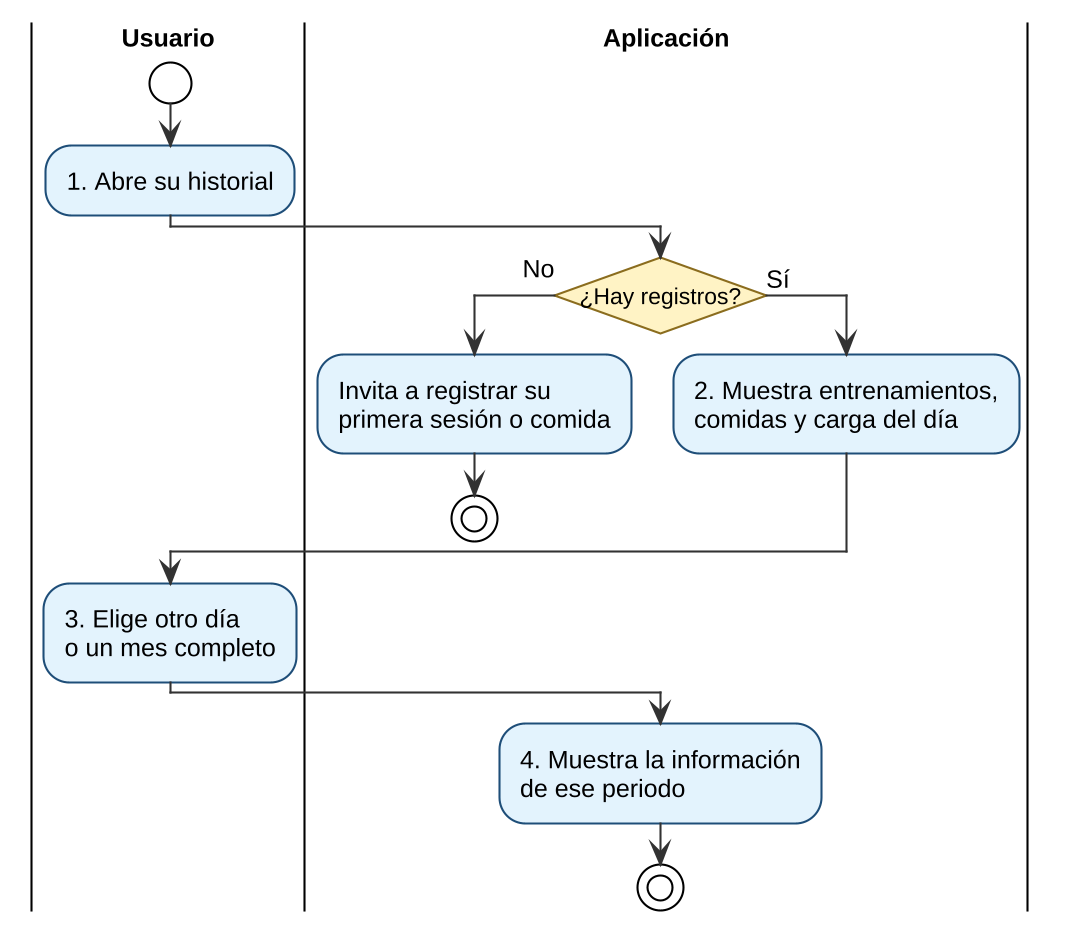
\includegraphics[width=0.78\textwidth,height=0.42\textheight,keepaspectratio]{figuras/diseno/dga_cu19.png}
    \captionof{figure}{Diagrama de Actividades -- CU-19: Revisar mi progreso.}
    \label{fig:dga_cu19}
\end{center}

\noindent\begin{minipage}{\linewidth}
\textbf{Descripción Esencial Expandida del Caso de Uso}
\par\vspace{0.2cm}
\noindent
{\renewcommand{\arraystretch}{1.25}\setstretch{1}\small
\begin{tabular}{|>{\raggedright\arraybackslash}p{2.9cm}|>{\raggedright\arraybackslash}p{12.1cm}|}
    \hline
    \rowcolor[HTML]{EFEFEF} \textbf{Propósito} & Ver en un solo lugar los entrenamientos, las comidas y la carga acumulada. \\ \hline
    \textbf{Tipo} & Primario \\ \hline
    \textbf{Actores} & Atleta Básico, Atleta Híbrido \\ \hline
    \textbf{Requerimientos} & R06 \\ \hline
    \textbf{Precondiciones} & El usuario inició sesión en la aplicación. \\ \hline
    \textbf{Poscondiciones} & El atleta ve su progreso. No se modifica ningún dato. \\ \hline
\end{tabular}

\vspace{0.15cm}
\noindent
\begin{tabular}{|>{\raggedright\arraybackslash}p{7.5cm}|>{\raggedright\arraybackslash}p{7.5cm}|}
    \hline
    \rowcolor[HTML]{D9E1F2} \multicolumn{2}{|c|}{\textbf{Curso Normal de los Eventos}} \\ \hline
    \rowcolor[HTML]{EFEFEF} \multicolumn{1}{|c|}{\textbf{Usuario}} & \multicolumn{1}{c|}{\textbf{Respuesta del Sistema}} \\ \hline
        1. Abre su historial. & 2. Muestra los entrenamientos, las comidas y la carga del día. \\ \hline
        3. Elige otro día o un mes completo. & 4. Muestra la información de ese periodo. \\ \hline
    \rowcolor[HTML]{F2D9D9} \multicolumn{2}{|c|}{\textbf{Cursos Alternos}} \\ \hline
    \rowcolor[HTML]{EFEFEF} \multicolumn{1}{|c|}{\textbf{Usuario}} & \multicolumn{1}{c|}{\textbf{Respuesta del Sistema}} \\ \hline
         & 2. Si todavía no hay registros, invita al atleta a registrar su primera sesión o comida. \\ \hline
\end{tabular}
}
\end{minipage}
\vspace{0.4cm}

\subsubsection{CU-20. Anotar cómo me sentí}

\textbf{Diagrama de Actividades}
\begin{center}
    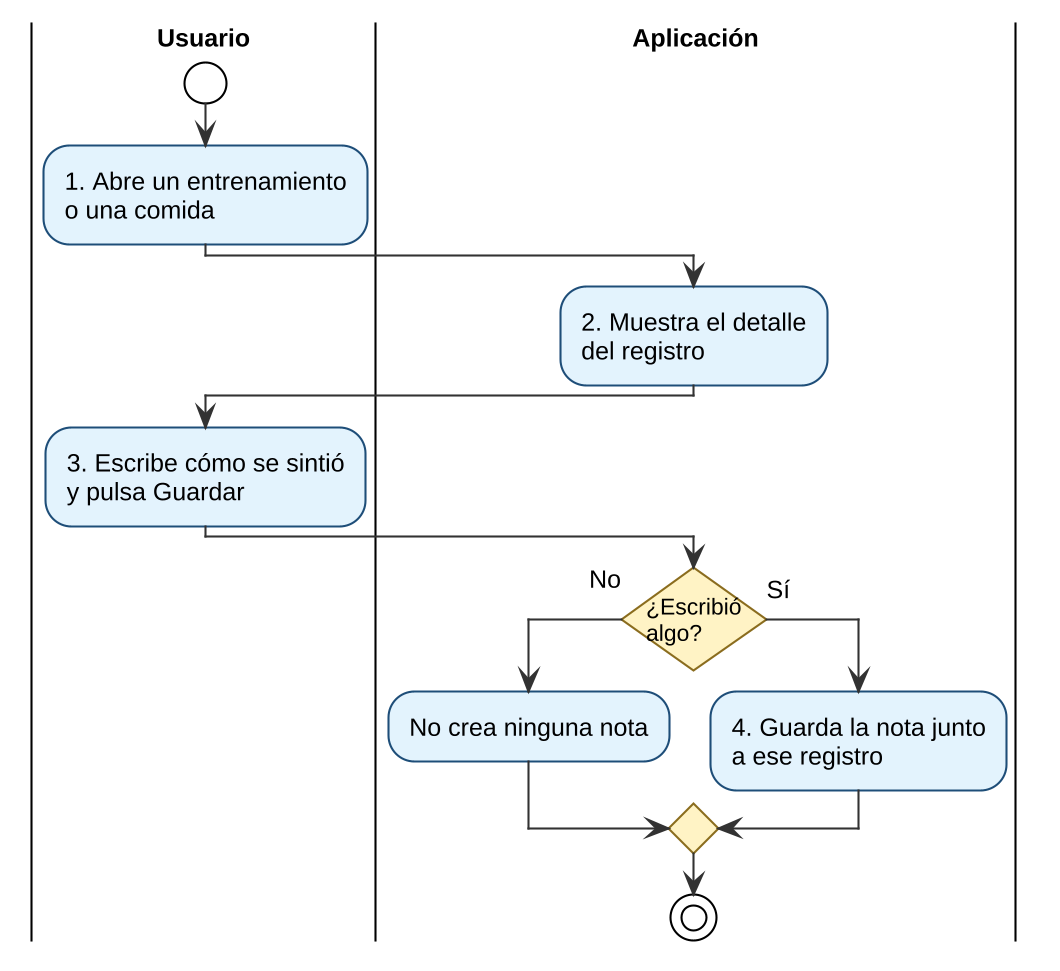
\includegraphics[width=0.78\textwidth,height=0.42\textheight,keepaspectratio]{figuras/diseno/dga_cu20.png}
    \captionof{figure}{Diagrama de Actividades -- CU-20: Anotar cómo me sentí.}
    \label{fig:dga_cu20}
\end{center}

\noindent\begin{minipage}{\linewidth}
\textbf{Descripción Esencial Expandida del Caso de Uso}
\par\vspace{0.2cm}
\noindent
{\renewcommand{\arraystretch}{1.25}\setstretch{1}\small
\begin{tabular}{|>{\raggedright\arraybackslash}p{2.9cm}|>{\raggedright\arraybackslash}p{12.1cm}|}
    \hline
    \rowcolor[HTML]{EFEFEF} \textbf{Propósito} & Guardar cómo se sintió el atleta física y digestivamente, para revisarlo después. \\ \hline
    \textbf{Tipo} & Primario \\ \hline
    \textbf{Actores} & Atleta Básico, Atleta Híbrido \\ \hline
    \textbf{Requerimientos} & R07 \\ \hline
    \textbf{Precondiciones} & El usuario inició sesión en la aplicación. Tiene un entrenamiento o una comida registrada. \\ \hline
    \textbf{Poscondiciones} & La nota queda junto al entrenamiento o la comida. \\ \hline
\end{tabular}

\vspace{0.15cm}
\noindent
\begin{tabular}{|>{\raggedright\arraybackslash}p{7.5cm}|>{\raggedright\arraybackslash}p{7.5cm}|}
    \hline
    \rowcolor[HTML]{D9E1F2} \multicolumn{2}{|c|}{\textbf{Curso Normal de los Eventos}} \\ \hline
    \rowcolor[HTML]{EFEFEF} \multicolumn{1}{|c|}{\textbf{Usuario}} & \multicolumn{1}{c|}{\textbf{Respuesta del Sistema}} \\ \hline
        1. Abre un entrenamiento o una comida. & 2. Muestra el detalle del registro. \\ \hline
        3. Escribe cómo se sintió y pulsa Guardar. & 4. Guarda la nota junto a ese registro. \\ \hline
    \rowcolor[HTML]{F2D9D9} \multicolumn{2}{|c|}{\textbf{Cursos Alternos}} \\ \hline
    \rowcolor[HTML]{EFEFEF} \multicolumn{1}{|c|}{\textbf{Usuario}} & \multicolumn{1}{c|}{\textbf{Respuesta del Sistema}} \\ \hline
        3. Si pulsa Guardar sin escribir nada, la aplicación no crea ninguna nota. &  \\ \hline
\end{tabular}
}
\end{minipage}
\vspace{0.4cm}

\subsubsection{CU-21. Controlar mis datos personales}

\textbf{Diagrama de Actividades}
\begin{center}
    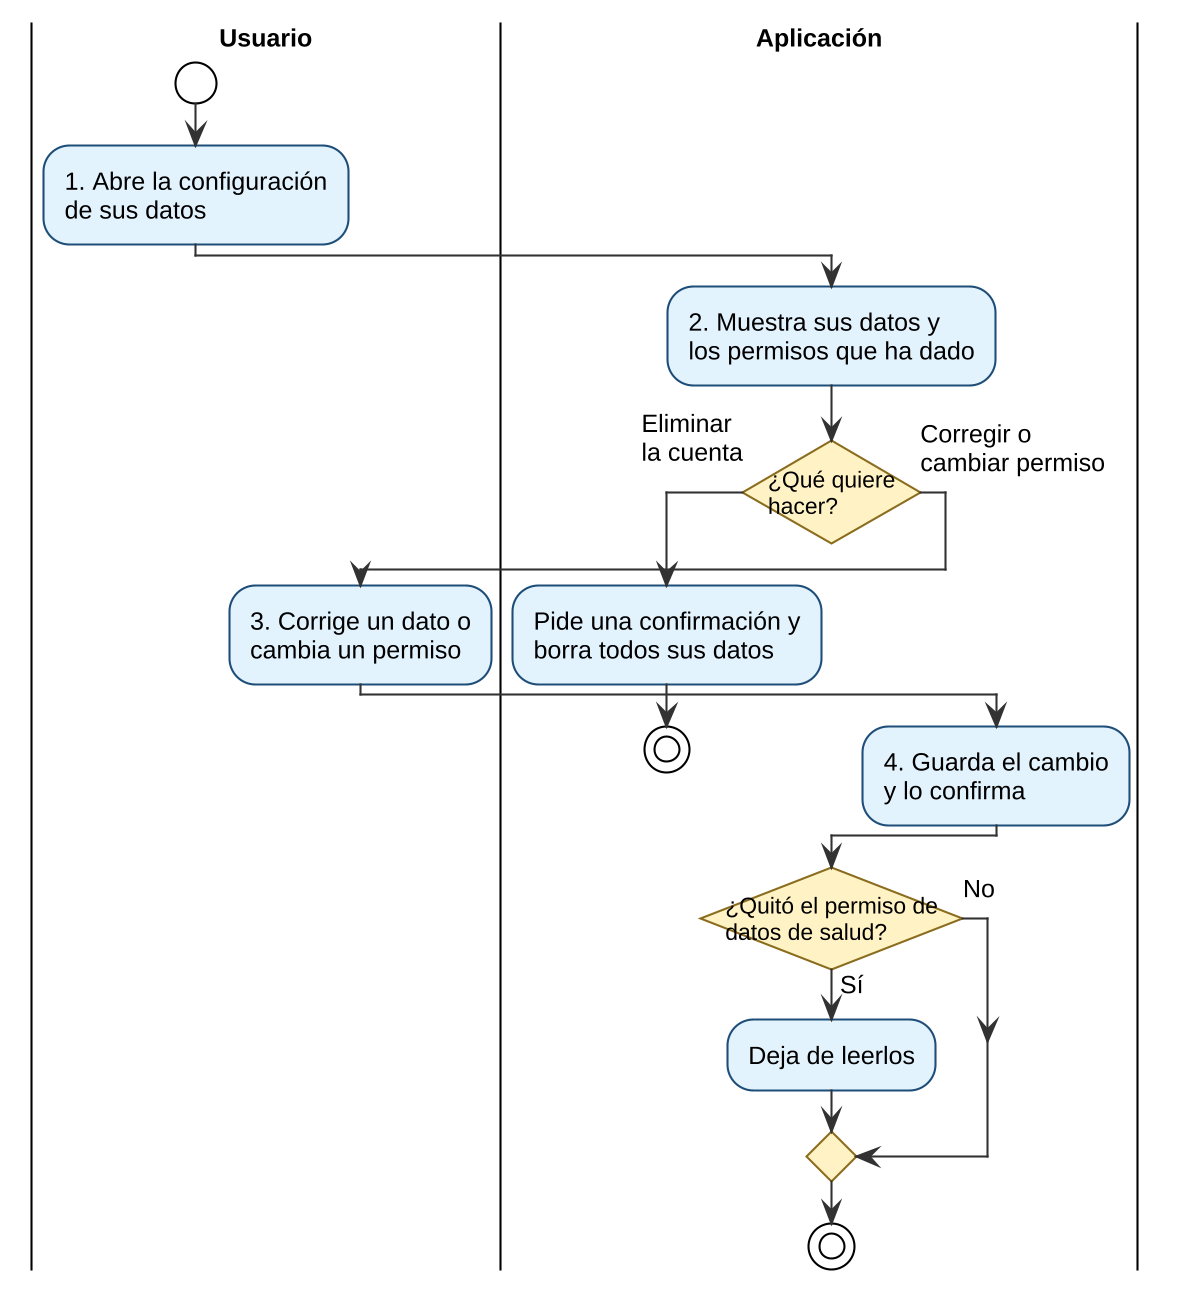
\includegraphics[width=0.78\textwidth,height=0.42\textheight,keepaspectratio]{figuras/diseno/dga_cu21.png}
    \captionof{figure}{Diagrama de Actividades -- CU-21: Controlar mis datos personales.}
    \label{fig:dga_cu21}
\end{center}

\noindent\begin{minipage}{\linewidth}
\textbf{Descripción Esencial Expandida del Caso de Uso}
\par\vspace{0.2cm}
\noindent
{\renewcommand{\arraystretch}{1.25}\setstretch{1}\small
\begin{tabular}{|>{\raggedright\arraybackslash}p{2.9cm}|>{\raggedright\arraybackslash}p{12.1cm}|}
    \hline
    \rowcolor[HTML]{EFEFEF} \textbf{Propósito} & Dar al atleta el control sobre sus datos, como pide la Ley N° 19.628. \\ \hline
    \textbf{Tipo} & Primario \\ \hline
    \textbf{Actores} & Atleta Básico, Atleta Híbrido, App de salud del teléfono \\ \hline
    \textbf{Requerimientos} & R09 \\ \hline
    \textbf{Precondiciones} & El usuario inició sesión en la aplicación. \\ \hline
    \textbf{Poscondiciones} & Los datos y los permisos quedan como el atleta los dejó. \\ \hline
\end{tabular}

\vspace{0.15cm}
\noindent
\begin{tabular}{|>{\raggedright\arraybackslash}p{7.5cm}|>{\raggedright\arraybackslash}p{7.5cm}|}
    \hline
    \rowcolor[HTML]{D9E1F2} \multicolumn{2}{|c|}{\textbf{Curso Normal de los Eventos}} \\ \hline
    \rowcolor[HTML]{EFEFEF} \multicolumn{1}{|c|}{\textbf{Usuario}} & \multicolumn{1}{c|}{\textbf{Respuesta del Sistema}} \\ \hline
        1. Abre la configuración de sus datos. & 2. Muestra sus datos y los permisos que ha dado. \\ \hline
        3. Corrige un dato o cambia un permiso. & 4. Guarda el cambio y lo confirma. \\ \hline
    \rowcolor[HTML]{F2D9D9} \multicolumn{2}{|c|}{\textbf{Cursos Alternos}} \\ \hline
    \rowcolor[HTML]{EFEFEF} \multicolumn{1}{|c|}{\textbf{Usuario}} & \multicolumn{1}{c|}{\textbf{Respuesta del Sistema}} \\ \hline
        3. Si quita el permiso a sus datos de salud, la aplicación deja de leerlos. &  \\ \hline
        3. Si elige eliminar su cuenta, la aplicación pide una confirmación y borra todos sus datos. &  \\ \hline
\end{tabular}
}
\end{minipage}
\vspace{0.4cm}

\subsubsection{CU-22. Reportar una publicación}

\textbf{Diagrama de Actividades}
\begin{center}
    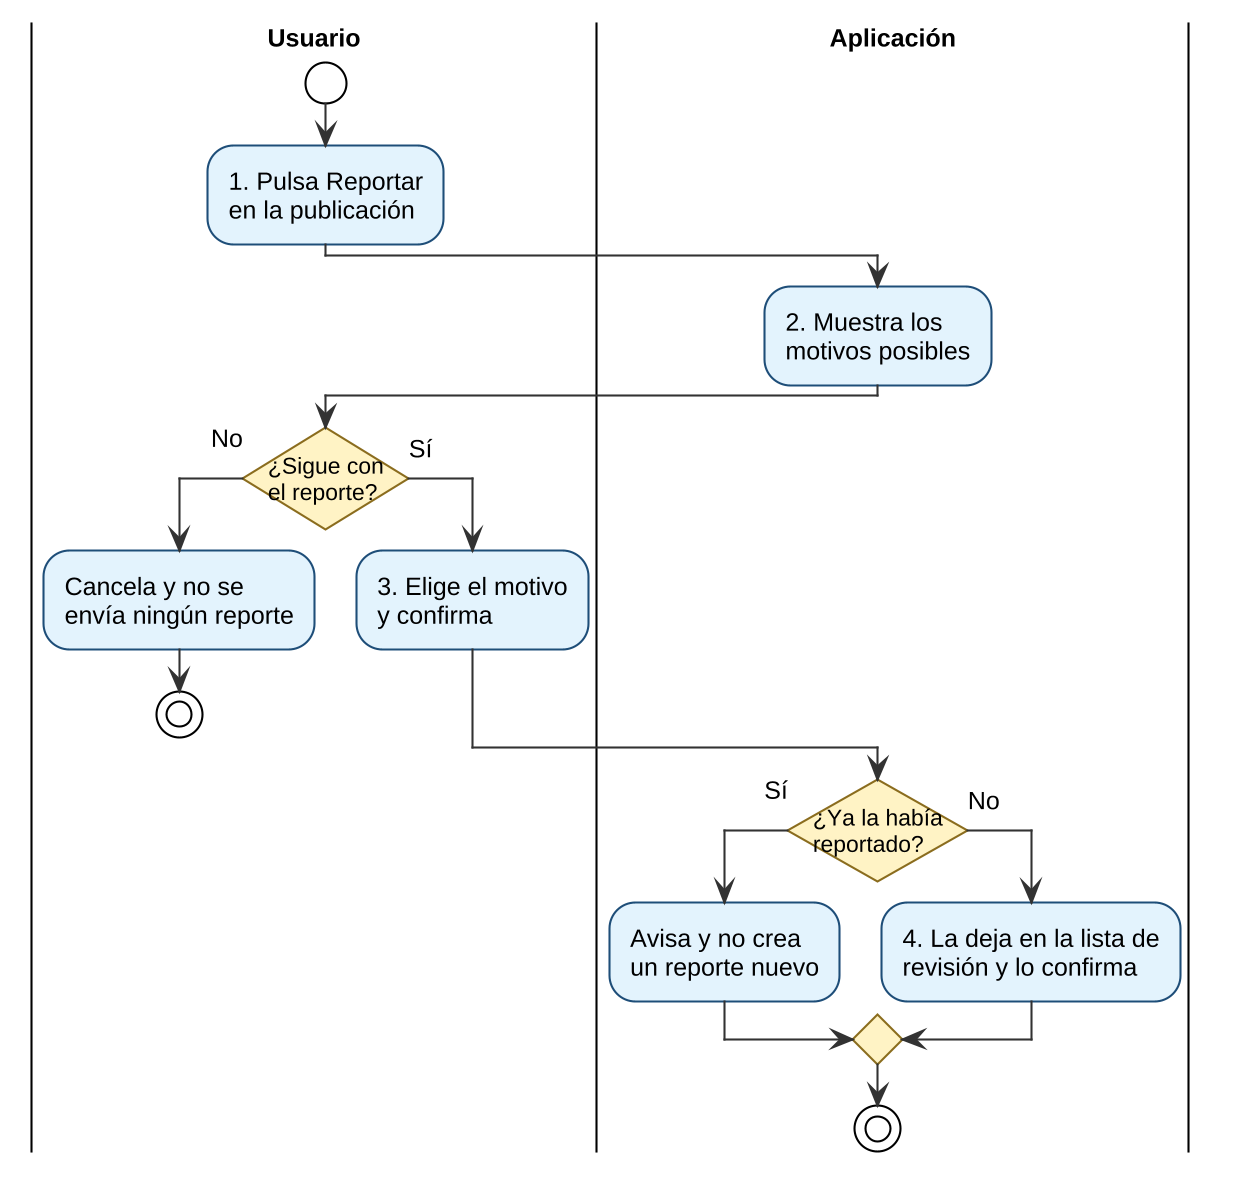
\includegraphics[width=0.78\textwidth,height=0.42\textheight,keepaspectratio]{figuras/diseno/dga_cu22.png}
    \captionof{figure}{Diagrama de Actividades -- CU-22: Reportar una publicación.}
    \label{fig:dga_cu22}
\end{center}

\noindent\begin{minipage}{\linewidth}
\textbf{Descripción Esencial Expandida del Caso de Uso}
\par\vspace{0.2cm}
\noindent
{\renewcommand{\arraystretch}{1.25}\setstretch{1}\small
\begin{tabular}{|>{\raggedright\arraybackslash}p{2.9cm}|>{\raggedright\arraybackslash}p{12.1cm}|}
    \hline
    \rowcolor[HTML]{EFEFEF} \textbf{Propósito} & Avisar al administrador de una publicación o foto inapropiada o peligrosa. \\ \hline
    \textbf{Tipo} & Primario \\ \hline
    \textbf{Actores} & Atleta Híbrido \\ \hline
    \textbf{Requerimientos} & R08, R11 \\ \hline
    \textbf{Precondiciones} & El usuario inició sesión y tiene el plan premium. Ve la publicación en su muro. \\ \hline
    \textbf{Poscondiciones} & La publicación queda en la lista de revisión del administrador (CU-11). \\ \hline
\end{tabular}

\vspace{0.15cm}
\noindent
\begin{tabular}{|>{\raggedright\arraybackslash}p{7.5cm}|>{\raggedright\arraybackslash}p{7.5cm}|}
    \hline
    \rowcolor[HTML]{D9E1F2} \multicolumn{2}{|c|}{\textbf{Curso Normal de los Eventos}} \\ \hline
    \rowcolor[HTML]{EFEFEF} \multicolumn{1}{|c|}{\textbf{Usuario}} & \multicolumn{1}{c|}{\textbf{Respuesta del Sistema}} \\ \hline
        1. Pulsa Reportar en la publicación. & 2. Muestra los motivos posibles. \\ \hline
        3. Elige el motivo y confirma. & 4. Deja la publicación en la lista de revisión y confirma el reporte. \\ \hline
    \rowcolor[HTML]{F2D9D9} \multicolumn{2}{|c|}{\textbf{Cursos Alternos}} \\ \hline
    \rowcolor[HTML]{EFEFEF} \multicolumn{1}{|c|}{\textbf{Usuario}} & \multicolumn{1}{c|}{\textbf{Respuesta del Sistema}} \\ \hline
        3. Si se arrepiente, puede cancelar y no se envía ningún reporte. &  \\ \hline
         & 4. Si ya la había reportado, avisa y no crea un reporte nuevo. \\ \hline
\end{tabular}
}
\end{minipage}
\vspace{0.4cm}

\subsubsection{CU-23. Ver el muro de la comunidad}

\textbf{Diagrama de Actividades}
\begin{center}
    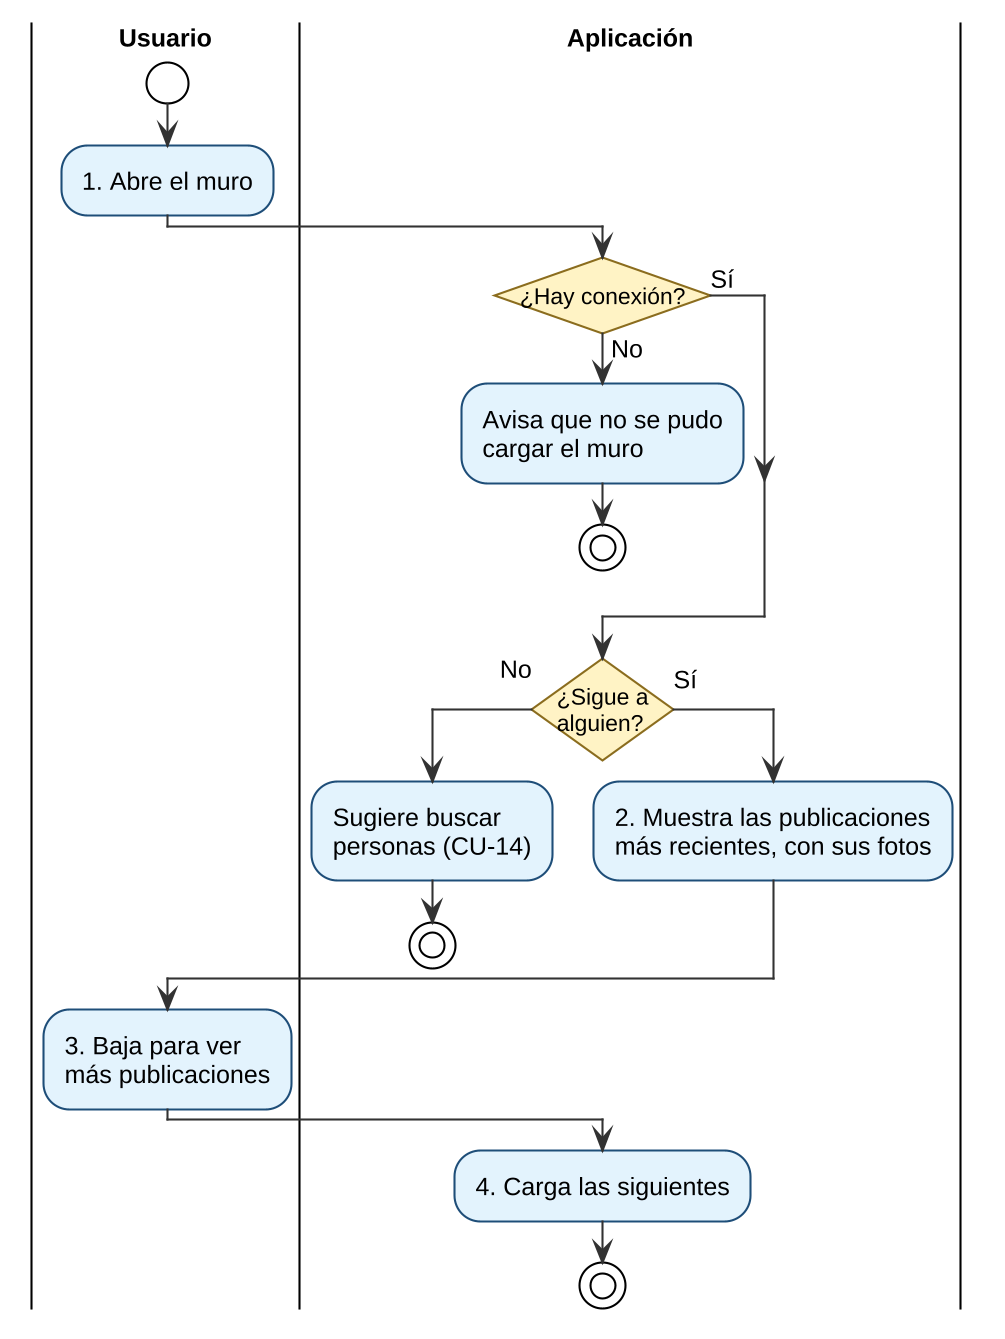
\includegraphics[width=0.78\textwidth,height=0.42\textheight,keepaspectratio]{figuras/diseno/dga_cu23.png}
    \captionof{figure}{Diagrama de Actividades -- CU-23: Ver el muro de la comunidad.}
    \label{fig:dga_cu23}
\end{center}

\noindent\begin{minipage}{\linewidth}
\textbf{Descripción Esencial Expandida del Caso de Uso}
\par\vspace{0.2cm}
\noindent
{\renewcommand{\arraystretch}{1.25}\setstretch{1}\small
\begin{tabular}{|>{\raggedright\arraybackslash}p{2.9cm}|>{\raggedright\arraybackslash}p{12.1cm}|}
    \hline
    \rowcolor[HTML]{EFEFEF} \textbf{Propósito} & Ver lo que publican las personas que el atleta sigue. \\ \hline
    \textbf{Tipo} & Primario \\ \hline
    \textbf{Actores} & Atleta Híbrido \\ \hline
    \textbf{Requerimientos} & R08 \\ \hline
    \textbf{Precondiciones} & El usuario inició sesión y tiene el plan premium. \\ \hline
    \textbf{Poscondiciones} & El atleta ve las publicaciones. Desde ahí puede agregarlas (CU-13) o reportarlas (CU-22). \\ \hline
\end{tabular}

\vspace{0.15cm}
\noindent
\begin{tabular}{|>{\raggedright\arraybackslash}p{7.5cm}|>{\raggedright\arraybackslash}p{7.5cm}|}
    \hline
    \rowcolor[HTML]{D9E1F2} \multicolumn{2}{|c|}{\textbf{Curso Normal de los Eventos}} \\ \hline
    \rowcolor[HTML]{EFEFEF} \multicolumn{1}{|c|}{\textbf{Usuario}} & \multicolumn{1}{c|}{\textbf{Respuesta del Sistema}} \\ \hline
        1. Abre el muro. & 2. Muestra las publicaciones más recientes que puede ver, con sus fotos. \\ \hline
        3. Baja para ver más publicaciones. & 4. Carga las siguientes. \\ \hline
    \rowcolor[HTML]{F2D9D9} \multicolumn{2}{|c|}{\textbf{Cursos Alternos}} \\ \hline
    \rowcolor[HTML]{EFEFEF} \multicolumn{1}{|c|}{\textbf{Usuario}} & \multicolumn{1}{c|}{\textbf{Respuesta del Sistema}} \\ \hline
         & 2. Si todavía no sigue a nadie, le sugiere buscar personas (CU-14). \\ \hline
         & 2. Si no hay conexión, avisa que no se pudo cargar el muro. \\ \hline
\end{tabular}
}
\end{minipage}
\vspace{0.4cm}

\subsubsection{CU-24. Contratar el plan premium}

\textbf{Diagrama de Actividades}
\begin{center}
    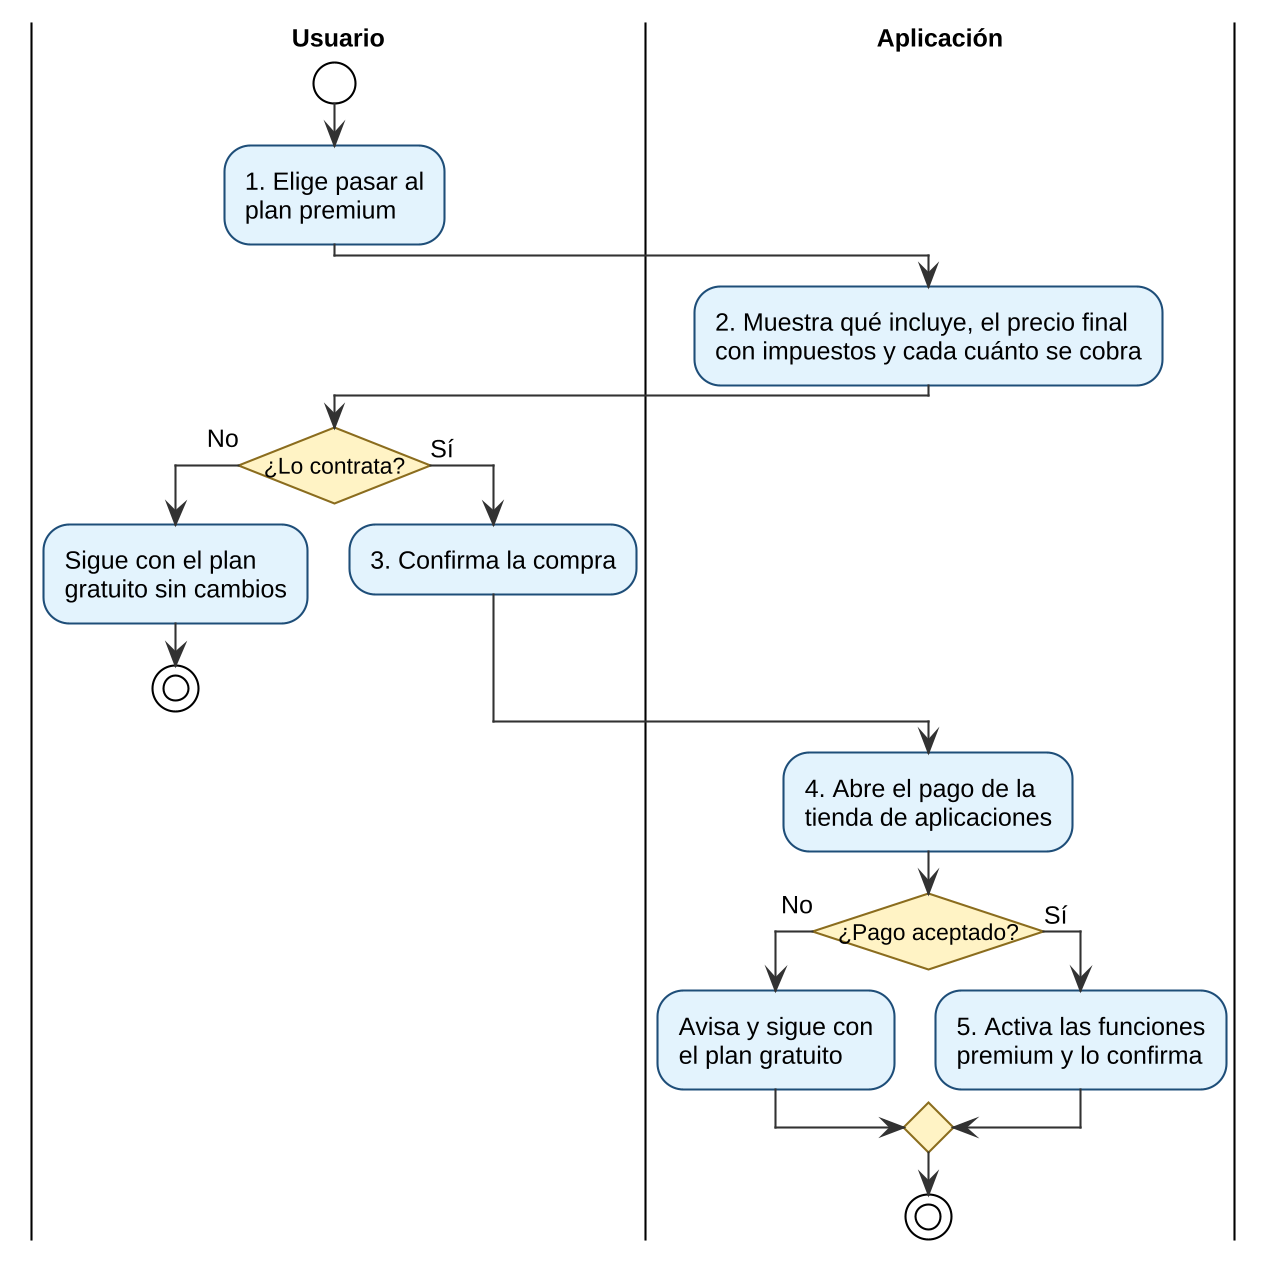
\includegraphics[width=0.78\textwidth,height=0.42\textheight,keepaspectratio]{figuras/diseno/dga_cu24.png}
    \captionof{figure}{Diagrama de Actividades -- CU-24: Contratar el plan premium.}
    \label{fig:dga_cu24}
\end{center}

\noindent\begin{minipage}{\linewidth}
\textbf{Descripción Esencial Expandida del Caso de Uso}
\par\vspace{0.2cm}
\noindent
{\renewcommand{\arraystretch}{1.25}\setstretch{1}\small
\begin{tabular}{|>{\raggedright\arraybackslash}p{2.9cm}|>{\raggedright\arraybackslash}p{12.1cm}|}
    \hline
    \rowcolor[HTML]{EFEFEF} \textbf{Propósito} & Permitir que el usuario acceda a todas las funciones pagando una suscripción. \\ \hline
    \textbf{Tipo} & Primario \\ \hline
    \textbf{Actores} & Atleta Básico \\ \hline
    \textbf{Requerimientos} & R14 \\ \hline
    \textbf{Precondiciones} & El usuario inició sesión y tiene el plan gratuito. \\ \hline
    \textbf{Poscondiciones} & El usuario tiene el plan premium activo. \\ \hline
\end{tabular}

\vspace{0.15cm}
\noindent
\begin{tabular}{|>{\raggedright\arraybackslash}p{7.5cm}|>{\raggedright\arraybackslash}p{7.5cm}|}
    \hline
    \rowcolor[HTML]{D9E1F2} \multicolumn{2}{|c|}{\textbf{Curso Normal de los Eventos}} \\ \hline
    \rowcolor[HTML]{EFEFEF} \multicolumn{1}{|c|}{\textbf{Usuario}} & \multicolumn{1}{c|}{\textbf{Respuesta del Sistema}} \\ \hline
        1. Elige pasar al plan premium. & 2. Muestra qué incluye, el precio final con impuestos y cada cuánto se cobra. \\ \hline
        3. Confirma la compra. & 4. Abre el pago de la tienda de aplicaciones. \\ \hline
         & 5. Activa las funciones premium y lo confirma. \\ \hline
    \rowcolor[HTML]{F2D9D9} \multicolumn{2}{|c|}{\textbf{Cursos Alternos}} \\ \hline
    \rowcolor[HTML]{EFEFEF} \multicolumn{1}{|c|}{\textbf{Usuario}} & \multicolumn{1}{c|}{\textbf{Respuesta del Sistema}} \\ \hline
        3. Si decide no contratar, sigue con el plan gratuito sin cambios. &  \\ \hline
         & 4. Si el pago es rechazado, avisa y el usuario sigue con el plan gratuito. \\ \hline
\end{tabular}
}
\end{minipage}
\vspace{0.4cm}

\subsubsection{CU-25. Cancelar mi suscripción}

\textbf{Diagrama de Actividades}
\begin{center}
    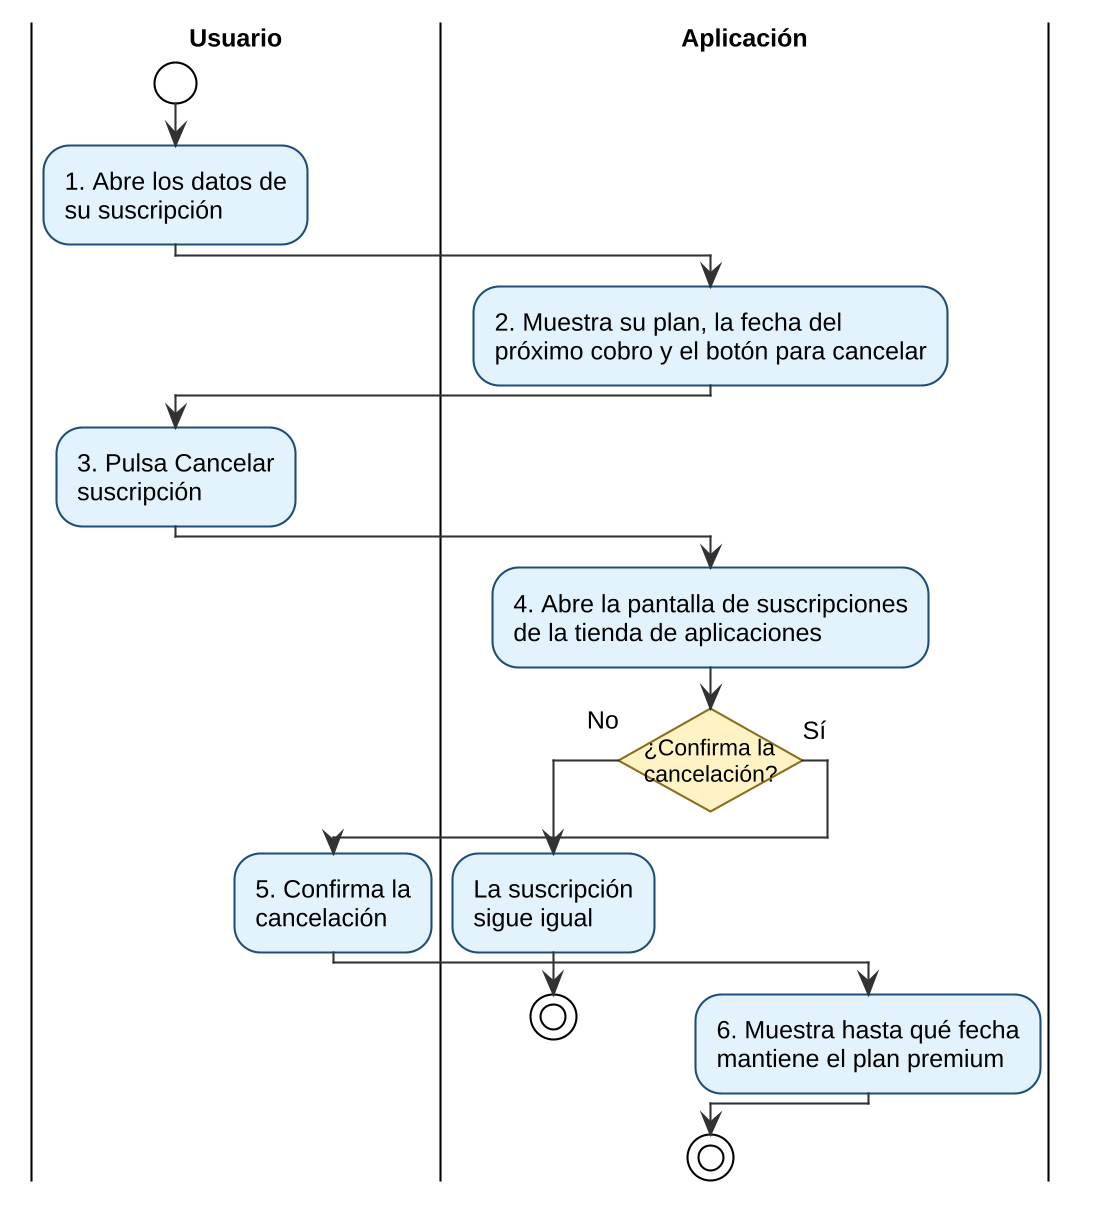
\includegraphics[width=0.78\textwidth,height=0.42\textheight,keepaspectratio]{figuras/diseno/dga_cu25.png}
    \captionof{figure}{Diagrama de Actividades -- CU-25: Cancelar mi suscripción.}
    \label{fig:dga_cu25}
\end{center}

\noindent\begin{minipage}{\linewidth}
\textbf{Descripción Esencial Expandida del Caso de Uso}
\par\vspace{0.2cm}
\noindent
{\renewcommand{\arraystretch}{1.25}\setstretch{1}\small
\begin{tabular}{|>{\raggedright\arraybackslash}p{2.9cm}|>{\raggedright\arraybackslash}p{12.1cm}|}
    \hline
    \rowcolor[HTML]{EFEFEF} \textbf{Propósito} & Permitir que el usuario deje de pagar la suscripción, como pide la Ley N° 19.496. \\ \hline
    \textbf{Tipo} & Primario \\ \hline
    \textbf{Actores} & Atleta Híbrido \\ \hline
    \textbf{Requerimientos} & R14 \\ \hline
    \textbf{Precondiciones} & El usuario inició sesión y tiene el plan premium. \\ \hline
    \textbf{Poscondiciones} & No hay nuevos cobros. Al terminar el periodo pagado, el usuario vuelve al plan gratuito y conserva sus datos. \\ \hline
\end{tabular}

\vspace{0.15cm}
\noindent
\begin{tabular}{|>{\raggedright\arraybackslash}p{7.5cm}|>{\raggedright\arraybackslash}p{7.5cm}|}
    \hline
    \rowcolor[HTML]{D9E1F2} \multicolumn{2}{|c|}{\textbf{Curso Normal de los Eventos}} \\ \hline
    \rowcolor[HTML]{EFEFEF} \multicolumn{1}{|c|}{\textbf{Usuario}} & \multicolumn{1}{c|}{\textbf{Respuesta del Sistema}} \\ \hline
        1. Abre los datos de su suscripción. & 2. Muestra su plan, la fecha del próximo cobro y el botón para cancelar. \\ \hline
        3. Pulsa Cancelar suscripción. & 4. Abre la pantalla de suscripciones de la tienda de aplicaciones. \\ \hline
        5. Confirma la cancelación. & 6. Muestra hasta qué fecha mantiene el plan premium. \\ \hline
    \rowcolor[HTML]{F2D9D9} \multicolumn{2}{|c|}{\textbf{Cursos Alternos}} \\ \hline
    \rowcolor[HTML]{EFEFEF} \multicolumn{1}{|c|}{\textbf{Usuario}} & \multicolumn{1}{c|}{\textbf{Respuesta del Sistema}} \\ \hline
        5. Si se arrepiente, no confirma y la suscripción sigue igual. &  \\ \hline
\end{tabular}
}
\end{minipage}
\vspace{0.4cm}

\subsubsection{CU-26. Aceptar los términos de uso y el aviso legal}

\textbf{Diagrama de Actividades}
\begin{center}
    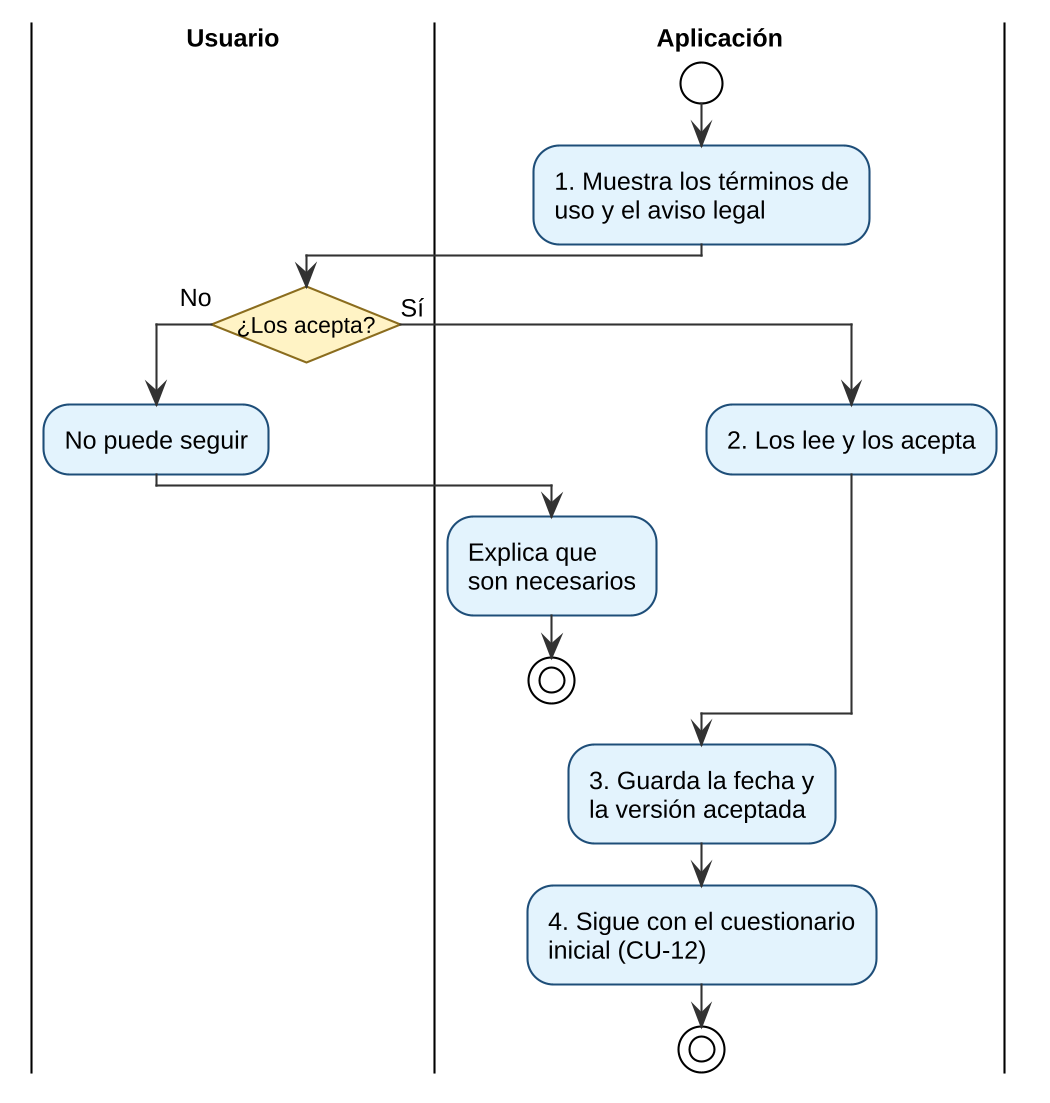
\includegraphics[width=0.78\textwidth,height=0.42\textheight,keepaspectratio]{figuras/diseno/dga_cu26.png}
    \captionof{figure}{Diagrama de Actividades -- CU-26: Aceptar los términos de uso y el aviso legal.}
    \label{fig:dga_cu26}
\end{center}

\noindent\begin{minipage}{\linewidth}
\textbf{Descripción Esencial Expandida del Caso de Uso}
\par\vspace{0.2cm}
\noindent
{\renewcommand{\arraystretch}{1.25}\setstretch{1}\small
\begin{tabular}{|>{\raggedright\arraybackslash}p{2.9cm}|>{\raggedright\arraybackslash}p{12.1cm}|}
    \hline
    \rowcolor[HTML]{EFEFEF} \textbf{Propósito} & Informar al usuario las condiciones de la aplicación y que esta no reemplaza a un profesional de la salud. \\ \hline
    \textbf{Tipo} & Primario \\ \hline
    \textbf{Actores} & Atleta Básico, Atleta Híbrido \\ \hline
    \textbf{Requerimientos} & R15 \\ \hline
    \textbf{Precondiciones} & El usuario está creando su cuenta. \\ \hline
    \textbf{Poscondiciones} & Queda registro de lo que aceptó el usuario. \\ \hline
\end{tabular}

\vspace{0.15cm}
\noindent
\begin{tabular}{|>{\raggedright\arraybackslash}p{7.5cm}|>{\raggedright\arraybackslash}p{7.5cm}|}
    \hline
    \rowcolor[HTML]{D9E1F2} \multicolumn{2}{|c|}{\textbf{Curso Normal de los Eventos}} \\ \hline
    \rowcolor[HTML]{EFEFEF} \multicolumn{1}{|c|}{\textbf{Usuario}} & \multicolumn{1}{c|}{\textbf{Respuesta del Sistema}} \\ \hline
         & 1. Muestra los términos de uso y el aviso legal. \\ \hline
        2. Los lee y los acepta. & 3. Guarda la fecha y la versión aceptada. \\ \hline
         & 4. Sigue con el cuestionario inicial (CU-12). \\ \hline
    \rowcolor[HTML]{F2D9D9} \multicolumn{2}{|c|}{\textbf{Cursos Alternos}} \\ \hline
    \rowcolor[HTML]{EFEFEF} \multicolumn{1}{|c|}{\textbf{Usuario}} & \multicolumn{1}{c|}{\textbf{Respuesta del Sistema}} \\ \hline
         & 1. Si los términos cambian más adelante, los vuelve a mostrar la próxima vez que el usuario entre. \\ \hline
        2. Si no los acepta, la aplicación explica que son necesarios y no permite seguir. &  \\ \hline
\end{tabular}
}
\end{minipage}
\vspace{0.4cm}

\subsubsection{CU-27. Crear una receta}

\textbf{Diagrama de Actividades}
\begin{center}
    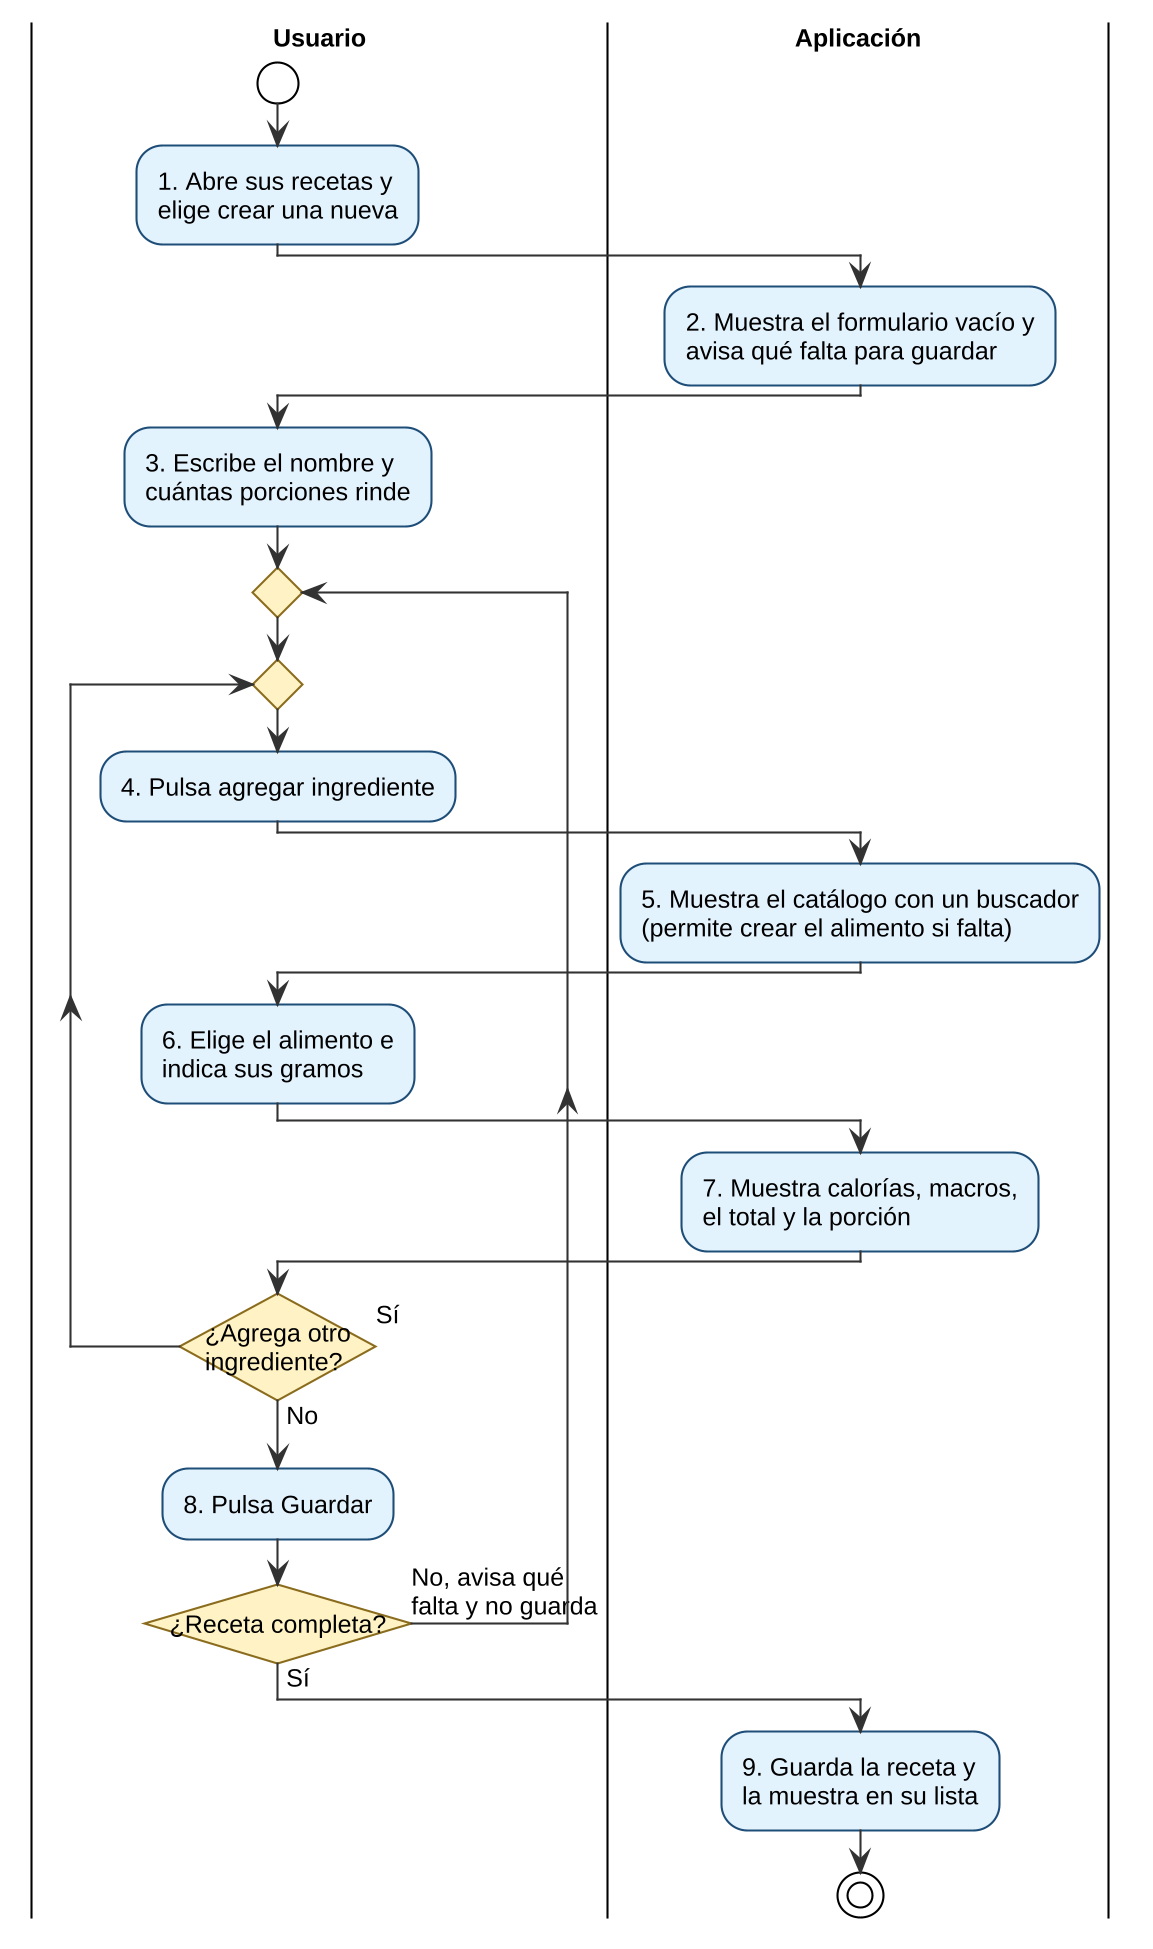
\includegraphics[width=0.9\textwidth,height=0.76\textheight,keepaspectratio]{figuras/diseno/dga_cu27.png}
    \captionof{figure}{Diagrama de Actividades -- CU-27: Crear una receta.}
    \label{fig:dga_cu27}
\end{center}

\noindent\begin{minipage}{\linewidth}
\textbf{Descripción Esencial Expandida del Caso de Uso}
\par\vspace{0.2cm}
\noindent
{\renewcommand{\arraystretch}{1.25}\setstretch{1}\small
\begin{tabular}{|>{\raggedright\arraybackslash}p{2.9cm}|>{\raggedright\arraybackslash}p{12.1cm}|}
    \hline
    \rowcolor[HTML]{EFEFEF} \textbf{Propósito} & Guardar una receta propia, con sus ingredientes y porciones, para volver a registrarla con un solo paso o compartirla. \\ \hline
    \textbf{Tipo} & Primario \\ \hline
    \textbf{Actores} & Atleta Básico, Atleta Híbrido \\ \hline
    \textbf{Requerimientos} & R04 \\ \hline
    \textbf{Precondiciones} & El usuario inició sesión en la aplicación. \\ \hline
    \textbf{Poscondiciones} & La receta queda guardada en el módulo de nutrición del atleta y se puede encontrar al buscar alimentos (CU-06). Un Atleta Híbrido puede publicarla (CU-09). \\ \hline
\end{tabular}

\vspace{0.15cm}
\noindent
\begin{tabular}{|>{\raggedright\arraybackslash}p{7.5cm}|>{\raggedright\arraybackslash}p{7.5cm}|}
    \hline
    \rowcolor[HTML]{D9E1F2} \multicolumn{2}{|c|}{\textbf{Curso Normal de los Eventos}} \\ \hline
    \rowcolor[HTML]{EFEFEF} \multicolumn{1}{|c|}{\textbf{Usuario}} & \multicolumn{1}{c|}{\textbf{Respuesta del Sistema}} \\ \hline
        1. Abre sus recetas y elige crear una nueva. & 2. Muestra el formulario vacío y avisa qué falta para poder guardar. \\ \hline
        3. Escribe el nombre y cuántas porciones rinde. &  \\ \hline
        4. Pulsa agregar ingrediente. & 5. Muestra el catálogo de alimentos con un buscador. \\ \hline
        6. Elige un alimento e indica cuántos gramos lleva. & 7. Muestra sus calorías y sus macronutrientes, y actualiza el total y lo que aporta cada porción. \\ \hline
        8. Repite los pasos 4 a 7 con cada ingrediente y pulsa Guardar. & 9. Revisa que la receta esté completa, la guarda y la muestra en su lista de recetas. \\ \hline
    \rowcolor[HTML]{F2D9D9} \multicolumn{2}{|c|}{\textbf{Cursos Alternos}} \\ \hline
    \rowcolor[HTML]{EFEFEF} \multicolumn{1}{|c|}{\textbf{Usuario}} & \multicolumn{1}{c|}{\textbf{Respuesta del Sistema}} \\ \hline
         & 5. Si el alimento no está en el catálogo, permite crearlo desde la misma búsqueda y lo agrega a la receta. \\ \hline
        7. Si se equivoca con un ingrediente, lo quita o cambia sus gramos, y el total se recalcula. &  \\ \hline
         & 9. Si falta el nombre, las porciones, algún ingrediente o los gramos de uno de ellos, no deja guardar y avisa qué falta. \\ \hline
\end{tabular}
}
\end{minipage}
\vspace{0.4cm}

\subsection{Diseño Técnico}
Esta sección aborda la estructura técnica interna del sistema, detallando cómo se organizan y relacionan las entidades de información, tanto a nivel de persistencia en base de datos como a nivel de la lógica de negocio en el backend.

\subsubsection{Modelo de Datos}

Para guardar la información de la aplicación se usará \textbf{MongoDB}, una base de datos NoSQL orientada a documentos. En vez de tablas, MongoDB organiza los datos en \textbf{colecciones} de \textbf{documentos}, que se guardan en formato BSON (JSON binario). Cada documento puede tener una estructura distinta, lo que se ajusta bien a los datos deportivos, donde una sesión de fuerza puede tener 3 ejercicios y otra 7, cada uno con distinta cantidad de series.
\\\\
El modelo sigue dos reglas simples:
\begin{itemize}
    \item \textbf{Embeber lo que se usa junto:} La información que siempre se consulta en conjunto se guarda dentro del mismo documento. Por ejemplo, las series de cada ejercicio quedan dentro de la sesión de fuerza, y los alimentos de una comida quedan dentro de la comida. Así, una sola consulta trae todo lo necesario.
    \item \textbf{Referenciar lo que se comparte o crece mucho:} Los datos que usan muchos documentos, como el catálogo de ejercicios o de alimentos, tienen su propia colección y se referencian por su identificador (\texttt{ObjectId}). Lo mismo pasa con la telemetría segundo a segundo, que se guarda en una colección de series temporales para no superar el tamaño máximo de un documento (16 MB).
\end{itemize}

Con estas reglas, el modelo queda formado por 15 colecciones, que se resumen en la Tabla \ref{tab:colecciones}.
\begin{table}[h!]
    \centering
    \renewcommand{\arraystretch}{1.3}
    \begin{tabular}{|p{3.0cm}|p{3.9cm}|p{7.5cm}|}
        \hline
        \rowcolor[HTML]{EFEFEF}
        \textbf{Módulo} & \textbf{Colección} & \textbf{Qué guarda} \\ \hline
        Identidad y acceso & \texttt{users} & Usuarios, con su perfil y sus integraciones embebidas. \\ \hline
        Registro diario & \texttt{dailyLogs} & Metas del día y reportes de sensaciones. \\ \hline
        Fuerza & \texttt{exercises} & Catálogo de ejercicios. \\ \hline
        Fuerza y cardio & \texttt{workouts} & Sesiones de fuerza (con ejercicios y series) y de resistencia. \\ \hline
        Cardio & \texttt{telemetry} & Serie temporal con los datos segundo a segundo. \\ \hline
        Nutrición & \texttt{foodItems} & Catálogo de alimentos, con su código de barras. \\ \hline
        Nutrición & \texttt{meals} & Comidas, con sus alimentos embebidos. \\ \hline
        Fatiga & \texttt{fatigueSnapshots} & Cálculo diario de carga y fatiga, con sus alertas. \\ \hline
        Nutrición y comunidad & \texttt{recipes} & Recetas propias o agregadas desde la comunidad, con sus ingredientes. \\ \hline
        Comunidad & \texttt{posts} & Publicaciones de sesiones, rutas y comidas en la red social. \\ \hline
        Perfil y plan & \texttt{trainingPlans} & Plan semanal sugerido de cada usuario y sus ajustes. \\ \hline
        Red social & \texttt{follows} & Relaciones entre seguidores. \\ \hline
        Red social y fuerza & \texttt{routines} & Rutinas de fuerza propias o agregadas desde la comunidad. \\ \hline
        Red social y cardio & \texttt{routes} & Rutas propias o agregadas desde la comunidad. \\ \hline
        Administración & \texttt{moderationLogs} & Acciones de moderación del administrador. \\ \hline
    \end{tabular}
    \caption{Colecciones del modelo de datos en MongoDB.}
    \label{tab:colecciones}
\end{table}
\textbf{Índices principales}

Para que las consultas más frecuentes sean rápidas, se definen los siguientes índices:
\begin{itemize}
    \item \texttt{users.email}: único, para el inicio de sesión.
    \item \texttt{dailyLogs (userId, date)} y \texttt{fatigueSnapshots (userId, date)}: únicos, para que haya un solo documento por usuario y día.
    \item \texttt{workouts (userId, startedAt)} y \texttt{meals (userId, consumedAt)}: para armar la línea de tiempo diaria y mensual.
    \item \texttt{foodItems.barcode}: único y disperso (solo para los alimentos que tienen código), para la lectura de códigos de barras.
    \item \texttt{telemetry}: colección de series temporales, con \texttt{timestamp} como campo de tiempo y \texttt{meta.workoutId} como campo de agrupación.
    \item \texttt{follows (followerId, followeeId)}: único, para que no se repita una misma relación entre seguidores.
    
    \item \texttt{posts (authorId, createdAt)}: para armar el muro con las publicaciones más recientes de las personas que el usuario sigue.
    \item \texttt{routes.startPoint}: índice geoespacial (\texttt{2dsphere}), para buscar rutas cercanas.
    \item \texttt{trainingPlans (userId, weekStart)}: para obtener el plan de la semana actual.
\end{itemize}

Las funciones de la red social que quedan para después del MVP, como los récords de tramo y los retos entre seguidores, necesitarán colecciones adicionales (por ejemplo \texttt{segments}, \texttt{segmentEfforts} y \texttt{challenges}), que se diseñarán en esas versiones.

\subsubsection{Diccionario de Datos}
A continuación se detalla la estructura de cada colección. Los campos que están dentro de un subdocumento se escriben con punto (por ejemplo, \texttt{profile.weightKg}), y los arreglos de subdocumentos se marcan con corchetes (por ejemplo, \texttt{sets[].reps}). Todos los documentos tienen un campo \texttt{\_id} de tipo \texttt{ObjectId}, que MongoDB genera automáticamente.
\\\\
\noindent\textbf{Colección: users} \\
Descripción: Guarda la identidad del usuario, su perfil físico y sus conexiones con servicios externos. El perfil y las integraciones van embebidos porque siempre se leen junto con el usuario.
{\footnotesize
\renewcommand{\arraystretch}{1.2}
\begin{longtable}{|>{\raggedright\arraybackslash}p{4.7cm}|>{\raggedright\arraybackslash}p{1.8cm}|>{\raggedright\arraybackslash}p{2.3cm}|>{\raggedright\arraybackslash}p{5.4cm}|}
    \hline
    \rowcolor[HTML]{EFEFEF}
    \textbf{Campo} & \textbf{Tipo} & \textbf{Atributo} & \textbf{Descripción} \\ \hline
    \endhead
    \_id & ObjectId & Obligatorio & Identificador único del usuario. \\ \hline
    email & String & Único & Correo de contacto e inicio de sesión. \\ \hline
    passwordHash & String & Obligatorio & Contraseña protegida con un algoritmo de hash. \\ \hline
    firstName & String & Obligatorio & Nombre del usuario. \\ \hline
    lastName & String & Obligatorio & Apellido del usuario. \\ \hline
    role & String & Obligatorio & Rol (ATHLETE\_FREE, ATHLETE\_PREMIUM o ADMIN). \\ \hline
    consent.\allowbreak dataProcessing & Boolean & Obligatorio & Aceptación del tratamiento de datos sensibles. \\ \hline
    consent.\allowbreak grantedAt & Date & Obligatorio & Fecha de la aceptación. \\ \hline
    consent.\allowbreak termsVersion & String & Obligatorio & Versión de los términos de uso aceptada. \\ \hline
    subscription & Object & Opcional & Datos de la suscripción al plan premium. \\ \hline
    subscription.\allowbreak status & String & Obligatorio & Estado (ACTIVE, CANCELED o EXPIRED). \\ \hline
    subscription.\allowbreak store & String & Obligatorio & Tienda donde se contrató (GOOGLE\_PLAY o APP\_STORE). \\ \hline
    subscription.\allowbreak expiresAt & Date & Obligatorio & Fecha en que termina el periodo pagado. \\ \hline
    subscription.\allowbreak purchaseToken & String & Obligatorio & Comprobante de compra entregado por la tienda. \\ \hline
    deviceTokens[] & Array & Opcional & Identificadores del teléfono del usuario para enviar notificaciones. \\ \hline
    profile & Object & Embebido & Perfil físico del usuario. \\ \hline
    profile.\allowbreak birthDate & Date & Obligatorio & Fecha de nacimiento. \\ \hline
    profile.\allowbreak gender & String & Obligatorio & Género (M, F u OTHER). \\ \hline
    profile.\allowbreak heightCm & Double & Obligatorio & Estatura en centímetros. \\ \hline
    profile.\allowbreak weightKg & Double & Obligatorio & Peso en kilogramos. \\ \hline
    profile.\allowbreak restingHeartRate & Int32 & Opcional & Frecuencia cardíaca en reposo. \\ \hline
    profile.\allowbreak maxHeartRate & Int32 & Opcional & Frecuencia cardíaca máxima. \\ \hline
    profile.\allowbreak activityLevel & String & Obligatorio & Nivel de actividad física. \\ \hline
    profile.\allowbreak primaryGoal & String & Obligatorio & Meta principal (fuerza, resistencia o recomposición). \\ \hline
    profile.\allowbreak experienceLevel & String & Obligatorio & Nivel declarado (BEGINNER, INTERMEDIATE o ADVANCED). \\ \hline
    profile.\allowbreak orientation & String & Obligatorio & Orientación calculada a partir del cuestionario (STRENGTH, ENDURANCE o BALANCED). \\ \hline
    profile.\allowbreak availableDays & Int32 & Obligatorio & Días por semana que puede entrenar. \\ \hline
    profile.\allowbreak equipment[]\allowbreak  & Array & Opcional & Equipamiento disponible (gimnasio, mancuernas, bicicleta, reloj, etc.). \\ \hline
    profile.\allowbreak disciplines[]\allowbreak  & Array & Obligatorio & Disciplinas que practica (fuerza, ciclismo, running o trekking). \\ \hline
    integrations[]\allowbreak  & Array & Embebido & Conexiones con servicios externos. \\ \hline
    integrations[]\allowbreak .\allowbreak provider & String & Obligatorio & Proveedor (APPLE\_HEALTH, HEALTH\_CONNECT, GARMIN o POLAR). \\ \hline
    integrations[]\allowbreak .\allowbreak accessTokenEnc & BinData & Obligatorio & Token de acceso cifrado (AES-256). \\ \hline
    integrations[]\allowbreak .\allowbreak refreshTokenEnc & BinData & Opcional & Token de renovación cifrado. \\ \hline
    integrations[]\allowbreak .\allowbreak tokenExpiresAt & Date & Obligatorio & Vencimiento del token. \\ \hline
    integrations[]\allowbreak .\allowbreak isActive & Boolean & Obligatorio & Indica si la conexión está activa. \\ \hline
    createdAt & Date & Obligatorio & Fecha de registro. \\ \hline
    updatedAt & Date & Obligatorio & Fecha de la última actualización. \\ \hline
    deletedAt & Date & Opcional & Fecha de eliminación lógica. \\ \hline
\end{longtable}
}
\noindent\textbf{Colección: dailyLogs} \\
Descripción: Representa un día del usuario. Guarda sus metas de calorías y macronutrientes y sus reportes de sensaciones. Hay un solo documento por usuario y fecha.
{\footnotesize
\renewcommand{\arraystretch}{1.2}
\begin{longtable}{|>{\raggedright\arraybackslash}p{4.7cm}|>{\raggedright\arraybackslash}p{1.8cm}|>{\raggedright\arraybackslash}p{2.3cm}|>{\raggedright\arraybackslash}p{5.4cm}|}
    \hline
    \rowcolor[HTML]{EFEFEF}
    \textbf{Campo} & \textbf{Tipo} & \textbf{Atributo} & \textbf{Descripción} \\ \hline
    \endhead
    \_id & ObjectId & Obligatorio & Identificador del registro diario. \\ \hline
    userId & ObjectId & Ref. users & Usuario dueño del registro. \\ \hline
    date & Date & Índice único con userId & Fecha del registro. \\ \hline
    targets.\allowbreak calories & Int32 & Obligatorio & Meta de calorías del día. \\ \hline
    targets.\allowbreak proteinG & Double & Obligatorio & Meta de proteínas (g). \\ \hline
    targets.\allowbreak carbsG & Double & Obligatorio & Meta de carbohidratos (g). \\ \hline
    targets.\allowbreak fatG & Double & Obligatorio & Meta de grasas (g). \\ \hline
    subjectiveReports[]\allowbreak  & Array & Embebido & Reportes de sensaciones del día. \\ \hline
    subjectiveReports[]\allowbreak .\allowbreak rpeGeneral & Int32 & Obligatorio & Esfuerzo percibido general (1 a 10). \\ \hline
    subjectiveReports[]\allowbreak .\allowbreak sleepQuality & Int32 & Opcional & Calidad del sueño (1 a 10). \\ \hline
    subjectiveReports[]\allowbreak .\allowbreak muscleSoreness & Int32 & Opcional & Dolor muscular (1 a 10). \\ \hline
    subjectiveReports[]\allowbreak .\allowbreak energyLevel & Int32 & Opcional & Nivel de energía (1 a 10). \\ \hline
    subjectiveReports[]\allowbreak .\allowbreak giDiscomfort & Boolean & Opcional & Presencia de malestar digestivo. \\ \hline
    subjectiveReports[]\allowbreak .\allowbreak freeNotes & String & Opcional & Notas libres. \\ \hline
    subjectiveReports[]\allowbreak .\allowbreak relatedTo & Object & Opcional & Entrenamiento o comida al que pertenece la nota (tipo e identificador). \\ \hline
    subjectiveReports[]\allowbreak .\allowbreak createdAt & Date & Obligatorio & Fecha del reporte. \\ \hline
    notes & String & Opcional & Notas del día. \\ \hline
    createdAt & Date & Obligatorio & Fecha de creación. \\ \hline
    updatedAt & Date & Obligatorio & Fecha de modificación. \\ \hline
\end{longtable}
}
\noindent\textbf{Colección: exercises} \\
Descripción: Catálogo de ejercicios de fuerza, tanto oficiales como creados por los usuarios. Los grupos musculares van dentro del documento, porque son pocos y casi no cambian.
{\footnotesize
\renewcommand{\arraystretch}{1.2}
\begin{longtable}{|>{\raggedright\arraybackslash}p{4.7cm}|>{\raggedright\arraybackslash}p{1.8cm}|>{\raggedright\arraybackslash}p{2.3cm}|>{\raggedright\arraybackslash}p{5.4cm}|}
    \hline
    \rowcolor[HTML]{EFEFEF}
    \textbf{Campo} & \textbf{Tipo} & \textbf{Atributo} & \textbf{Descripción} \\ \hline
    \endhead
    \_id & ObjectId & Obligatorio & Identificador del ejercicio. \\ \hline
    name & String & Índice & Nombre del ejercicio. \\ \hline
    muscleGroups.\allowbreak primary & String & Obligatorio & Grupo muscular principal. \\ \hline
    muscleGroups.\allowbreak secondary & String & Opcional & Grupo muscular secundario. \\ \hline
    bodyRegion & String & Obligatorio & Región del cuerpo (UPPER, LOWER, CORE o FULL\_BODY). \\ \hline
    movementPattern & String & Obligatorio & Patrón de movimiento (PUSH, PULL, SQUAT, etc.). \\ \hline
    equipment & String & Obligatorio & Equipamiento requerido. \\ \hline
    measureType & String & Obligatorio & Forma de medir: REPS (repeticiones) o TIME (isométricos). \\ \hline
    isBodyweight & Boolean & Obligatorio & Indica si usa el peso corporal como carga (calistenia). \\ \hline
    description & String & Opcional & Instrucciones técnicas. \\ \hline
    isOfficial & Boolean & Obligatorio & Indica si pertenece al catálogo oficial. \\ \hline
    createdBy & ObjectId & Ref. users, opcional & Usuario que lo creó, si es personalizado. \\ \hline
    isActive & Boolean & Obligatorio & Estado del ejercicio. \\ \hline
    createdAt & Date & Obligatorio & Fecha de creación. \\ \hline
\end{longtable}
}
\noindent\textbf{Colección: workouts} \\
Descripción: Guarda todas las sesiones de entrenamiento. El campo \texttt{type} indica si es de fuerza o de resistencia, y según eso el documento tiene unos campos u otros. Esta flexibilidad es una de las ventajas del modelo de documentos.
{\footnotesize
\renewcommand{\arraystretch}{1.2}
\begin{longtable}{|>{\raggedright\arraybackslash}p{4.7cm}|>{\raggedright\arraybackslash}p{1.8cm}|>{\raggedright\arraybackslash}p{2.3cm}|>{\raggedright\arraybackslash}p{5.4cm}|}
    \hline
    \rowcolor[HTML]{EFEFEF}
    \textbf{Campo} & \textbf{Tipo} & \textbf{Atributo} & \textbf{Descripción} \\ \hline
    \endhead
    \multicolumn{4}{|l|}{\cellcolor[HTML]{E3F2FD}\textbf{Campos comunes}} \\ \hline
    \_id & ObjectId & Obligatorio & Identificador de la sesión. \\ \hline
    userId & ObjectId & Ref. users, índice & Usuario que realizó la sesión. \\ \hline
    dailyLogId & ObjectId & Ref. dailyLogs & Día al que pertenece la sesión. \\ \hline
    type & String & Obligatorio & Tipo de sesión (STRENGTH o CARDIO). \\ \hline
    startedAt & Date & Índice con userId & Inicio de la sesión. \\ \hline
    finishedAt & Date & Opcional & Fin de la sesión. \\ \hline
    sessionRpe & Int32 & Obligatorio & Esfuerzo percibido de la sesión (1 a 10), indicado por el usuario o estimado por la aplicación. \\ \hline
    rpeSource & String & Obligatorio & Origen del RPE: USER (lo indicó el usuario) o ESTIMATED (lo estimó la aplicación). \\ \hline
    loadAu & Double & Obligatorio & Carga de la sesión en unidades arbitrarias: RPE por minutos. \\ \hline
    notes & String & Opcional & Notas de la sesión. \\ \hline
    createdAt & Date & Obligatorio & Fecha de registro. \\ \hline
    \multicolumn{4}{|l|}{\cellcolor[HTML]{E3F2FD}\textbf{Solo cuando type = STRENGTH}} \\ \hline
    trainingType & String & Opcional & Tipo de fuerza (MAX\_STRENGTH, HYPERTROPHY, POWER, MUSCULAR\_ENDURANCE, ISOMETRIC o CALISTHENICS). \\ \hline
    inputMethod & String & Obligatorio & Forma de registro (MANUAL o NLP). \\ \hline
    nlpRawInput & String & Opcional & Texto original si se registró con lenguaje natural. \\ \hline
    totalVolumeKg & Double & Obligatorio & Volumen total (series por repeticiones por peso), solo informativo. \\ \hline
    exercises[]\allowbreak  & Array & Embebido & Ejercicios realizados en la sesión. \\ \hline
    exercises[]\allowbreak .\allowbreak exerciseId & ObjectId & Ref. exercises & Ejercicio del catálogo. \\ \hline
    exercises[]\allowbreak .\allowbreak exerciseName & String & Obligatorio & Copia del nombre, para mostrarlo sin consultar el catálogo. \\ \hline
    exercises[]\allowbreak .\allowbreak order & Int32 & Obligatorio & Orden de ejecución. \\ \hline
    exercises[]\allowbreak .\allowbreak sets[]\allowbreak  & Array & Embebido & Series del ejercicio. \\ \hline
    exercises[]\allowbreak .\allowbreak sets[]\allowbreak .\allowbreak reps & Int32 & Opcional & Repeticiones (no aplica en isométricos). \\ \hline
    exercises[]\allowbreak .\allowbreak sets[]\allowbreak .\allowbreak durationSec & Int32 & Opcional & Duración en segundos (isométricos). \\ \hline
    exercises[]\allowbreak .\allowbreak sets[]\allowbreak .\allowbreak weightKg & Double & Obligatorio & Carga en kilogramos, o lastre en calistenia. \\ \hline
    exercises[]\allowbreak .\allowbreak sets[]\allowbreak .\allowbreak rpe & Double & Opcional & Esfuerzo percibido de la serie. \\ \hline
    exercises[]\allowbreak .\allowbreak sets[]\allowbreak .\allowbreak restSec & Int32 & Opcional & Descanso en segundos. \\ \hline
    exercises[]\allowbreak .\allowbreak sets[]\allowbreak .\allowbreak isWarmup & Boolean & Opcional & Indica si fue una serie de calentamiento. \\ \hline
    \multicolumn{4}{|l|}{\cellcolor[HTML]{E3F2FD}\textbf{Solo cuando type = CARDIO}} \\ \hline
    discipline & String & Obligatorio & Disciplina (CYCLING, RUNNING o TREKKING). \\ \hline
    durationSec & Int32 & Obligatorio & Duración activa en segundos. \\ \hline
    distanceM & Double & Obligatorio & Distancia total en metros. \\ \hline
    avgSpeedKmh & Double & Opcional & Velocidad promedio. \\ \hline
    elevationGainM & Double & Opcional & Desnivel positivo en metros. \\ \hline
    dataSource & String & Obligatorio & Origen de los datos (PHONE\_GPS, HEALTH\_BROKER o FIT\_FILE). \\ \hline
    dataConfidence & String & Obligatorio & Nivel de confianza del dato (LOW, MEDIUM o HIGH). \\ \hline
    heartRate.\allowbreak avg & Int32 & Opcional & Frecuencia cardíaca promedio. \\ \hline
    heartRate.\allowbreak max & Int32 & Opcional & Frecuencia cardíaca máxima. \\ \hline
    heartRate.\allowbreak activeCalories & Int32 & Opcional & Calorías activas (kcal). \\ \hline
    power.\allowbreak avgWatts & Int32 & Opcional & Potencia promedio (W). \\ \hline
    power.\allowbreak maxWatts & Int32 & Opcional & Potencia máxima (W). \\ \hline
    power.\allowbreak normalizedPower & Int32 & Opcional & Potencia normalizada (NP). \\ \hline
    power.\allowbreak avgCadence & Int32 & Opcional & Cadencia promedio. \\ \hline
    power.\allowbreak tss & Double & Opcional & Training Stress Score, solo informativo. \\ \hline
    fitFileUrl & String & Opcional & Ubicación en S3 del archivo .fit original. \\ \hline
\end{longtable}
}
\noindent\textbf{Colección: telemetry} \\
Descripción: Colección de series temporales (time series) de MongoDB. Cada documento es una medición segundo a segundo de una sesión de resistencia. Se separa de \texttt{workouts} porque una sesión larga puede tener miles de puntos y un documento no puede superar los 16 MB.
{\footnotesize
\renewcommand{\arraystretch}{1.2}
\begin{longtable}{|>{\raggedright\arraybackslash}p{4.7cm}|>{\raggedright\arraybackslash}p{1.8cm}|>{\raggedright\arraybackslash}p{2.3cm}|>{\raggedright\arraybackslash}p{5.4cm}|}
    \hline
    \rowcolor[HTML]{EFEFEF}
    \textbf{Campo} & \textbf{Tipo} & \textbf{Atributo} & \textbf{Descripción} \\ \hline
    \endhead
    \_id & ObjectId & Obligatorio & Identificador de la medición. \\ \hline
    timestamp & Date & Campo de tiempo & Momento de la medición. \\ \hline
    meta.\allowbreak workoutId & ObjectId & Ref. workouts & Sesión a la que pertenece la medición. \\ \hline
    meta.\allowbreak userId & ObjectId & Ref. users & Usuario dueño de la sesión. \\ \hline
    meta.\allowbreak source & String & Obligatorio & Origen (FIT\_FILE o HEALTH\_BROKER). \\ \hline
    heartRate & Int32 & Opcional & Frecuencia cardíaca. \\ \hline
    powerWatts & Int32 & Opcional & Potencia (W). \\ \hline
    cadence & Int32 & Opcional & Cadencia. \\ \hline
    speedKmh & Double & Opcional & Velocidad. \\ \hline
    altitudeM & Double & Opcional & Altitud en metros. \\ \hline
    location & Object & Opcional & Posición GPS en formato GeoJSON (punto). \\ \hline
\end{longtable}
}
\noindent\textbf{Colección: foodItems} \\
Descripción: Catálogo de alimentos, ya sea cargados desde una base externa (como OpenFoodFacts), creados por los usuarios o estimados por la IA.
{\footnotesize
\renewcommand{\arraystretch}{1.2}
\begin{longtable}{|>{\raggedright\arraybackslash}p{4.7cm}|>{\raggedright\arraybackslash}p{1.8cm}|>{\raggedright\arraybackslash}p{2.3cm}|>{\raggedright\arraybackslash}p{5.4cm}|}
    \hline
    \rowcolor[HTML]{EFEFEF}
    \textbf{Campo} & \textbf{Tipo} & \textbf{Atributo} & \textbf{Descripción} \\ \hline
    \endhead
    \_id & ObjectId & Obligatorio & Identificador del alimento. \\ \hline
    name & String & Índice de texto & Nombre del alimento. \\ \hline
    brand & String & Opcional & Marca o fabricante. \\ \hline
    servingSizeG & Double & Obligatorio & Tamaño de la porción estándar (g). \\ \hline
    per100g.\allowbreak calories & Double & Obligatorio & Calorías por cada 100 g. \\ \hline
    per100g.\allowbreak proteinG & Double & Obligatorio & Proteínas por cada 100 g. \\ \hline
    per100g.\allowbreak carbsG & Double & Obligatorio & Carbohidratos por cada 100 g. \\ \hline
    per100g.\allowbreak fatG & Double & Obligatorio & Grasas por cada 100 g. \\ \hline
    per100g.\allowbreak fiberG & Double & Opcional & Fibra por cada 100 g. \\ \hline
    source & String & Obligatorio & Origen (OPEN\_FOOD\_FACTS, USER o AI). \\ \hline
    barcode & String & Único, opcional & Código de barras EAN o UPC. \\ \hline
    isActive & Boolean & Obligatorio & Estado del alimento. \\ \hline
    createdAt & Date & Obligatorio & Fecha de alta. \\ \hline
\end{longtable}
}
\noindent\textbf{Colección: meals} \\
Descripción: Registro de cada comida. Los alimentos consumidos van dentro del documento, junto con los totales ya calculados, para mostrar el diario sin consultas adicionales.
{\footnotesize
\renewcommand{\arraystretch}{1.2}
\begin{longtable}{|>{\raggedright\arraybackslash}p{4.7cm}|>{\raggedright\arraybackslash}p{1.8cm}|>{\raggedright\arraybackslash}p{2.3cm}|>{\raggedright\arraybackslash}p{5.4cm}|}
    \hline
    \rowcolor[HTML]{EFEFEF}
    \textbf{Campo} & \textbf{Tipo} & \textbf{Atributo} & \textbf{Descripción} \\ \hline
    \endhead
    \_id & ObjectId & Obligatorio & Identificador de la comida. \\ \hline
    userId & ObjectId & Ref. users, índice & Usuario que registró la comida. \\ \hline
    dailyLogId & ObjectId & Ref. dailyLogs & Día al que descuenta los macronutrientes. \\ \hline
    mealType & String & Obligatorio & Momento (BREAKFAST, LUNCH, DINNER o SNACK). \\ \hline
    inputMethod & String & Obligatorio & Forma de registro (MANUAL, TEXT, PHOTO o BARCODE). \\ \hline
    aiConfidenceScore & Double & Opcional & Seguridad de la estimación de la IA (0 a 100). \\ \hline
    items[]\allowbreak  & Array & Embebido & Alimentos de la comida. \\ \hline
    items[]\allowbreak .\allowbreak foodItemId & ObjectId & Ref. foodItems & Alimento del catálogo. \\ \hline
    items[]\allowbreak .\allowbreak name & String & Obligatorio & Copia del nombre del alimento. \\ \hline
    items[]\allowbreak .\allowbreak quantityG & Double & Obligatorio & Gramos consumidos. \\ \hline
    items[]\allowbreak .\allowbreak calories & Double & Obligatorio & Calorías aportadas. \\ \hline
    items[]\allowbreak .\allowbreak proteinG & Double & Obligatorio & Proteínas aportadas. \\ \hline
    items[]\allowbreak .\allowbreak carbsG & Double & Obligatorio & Carbohidratos aportados. \\ \hline
    items[]\allowbreak .\allowbreak fatG & Double & Obligatorio & Grasas aportadas. \\ \hline
    totals.\allowbreak calories & Double & Obligatorio & Calorías totales de la comida. \\ \hline
    totals.\allowbreak proteinG & Double & Obligatorio & Proteínas totales. \\ \hline
    totals.\allowbreak carbsG & Double & Obligatorio & Carbohidratos totales. \\ \hline
    totals.\allowbreak fatG & Double & Obligatorio & Grasas totales. \\ \hline
    recipeRef.\allowbreak recipeId & ObjectId & Ref. recipes, opcional & Receta de la comunidad, si se importó. \\ \hline
    recipeRef.\allowbreak scaleFactor & Double & Opcional & Factor con el que se ajustó la receta. \\ \hline
    notes & String & Opcional & Notas de preparación. \\ \hline
    consumedAt & Date & Índice con userId & Momento en que se comió. \\ \hline
    createdAt & Date & Obligatorio & Fecha de registro. \\ \hline
\end{longtable}
}
\noindent\textbf{Colección: fatigueSnapshots} \\
Descripción: Guarda el cálculo diario de carga y fatiga de cada usuario. Las alertas que genera el cálculo van dentro del mismo documento.
{\footnotesize
\renewcommand{\arraystretch}{1.2}
\begin{longtable}{|>{\raggedright\arraybackslash}p{4.7cm}|>{\raggedright\arraybackslash}p{1.8cm}|>{\raggedright\arraybackslash}p{2.3cm}|>{\raggedright\arraybackslash}p{5.4cm}|}
    \hline
    \rowcolor[HTML]{EFEFEF}
    \textbf{Campo} & \textbf{Tipo} & \textbf{Atributo} & \textbf{Descripción} \\ \hline
    \endhead
    \_id & ObjectId & Obligatorio & Identificador del cálculo. \\ \hline
    userId & ObjectId & Ref. users & Usuario evaluado. \\ \hline
    date & Date & Índice único con userId & Fecha evaluada. \\ \hline
    strength.\allowbreak ctl & Double & Obligatorio & Carga crónica de fuerza. \\ \hline
    strength.\allowbreak atl & Double & Obligatorio & Carga aguda de fuerza. \\ \hline
    strength.\allowbreak tsb & Double & Obligatorio & Balance de forma (TSB) de fuerza. \\ \hline
    cardio.\allowbreak ctl & Double & Obligatorio & Carga crónica de resistencia. \\ \hline
    cardio.\allowbreak atl & Double & Obligatorio & Carga aguda de resistencia. \\ \hline
    cardio.\allowbreak tsb & Double & Obligatorio & Balance de forma (TSB) de resistencia. \\ \hline
    total.\allowbreak ctl & Double & Obligatorio & Carga crónica total (fuerza más cardio). \\ \hline
    total.\allowbreak atl & Double & Obligatorio & Carga aguda total (fuerza más cardio). \\ \hline
    total.\allowbreak tsb & Double & Obligatorio & Balance de forma (TSB) total. \\ \hline
    crossFatigueIndex & Double & Opcional & Índice de fatiga cruzada: razón ATL/CTL de la carga total (Tabla \ref{tab:def_operativas}). Queda vacío mientras no hay 28 días de historial. \\ \hline
    calculatedAt & Date & Obligatorio & Momento del cálculo. \\ \hline
    alerts[]\allowbreak  & Array & Embebido & Alertas generadas por el cálculo. \\ \hline
    alerts[]\allowbreak .\allowbreak alertType & String & Obligatorio & Tipo de alerta (CROSS\_FATIGUE, etc.). \\ \hline
    alerts[]\allowbreak .\allowbreak severity & String & Obligatorio & Severidad (INFO, WARNING o CRITICAL). \\ \hline
    alerts[]\allowbreak .\allowbreak message & String & Obligatorio & Mensaje de la alerta. \\ \hline
    alerts[]\allowbreak .\allowbreak suggestion & String & Opcional & Sugerencia de ajuste del entrenamiento. \\ \hline
    alerts[]\allowbreak .\allowbreak isRead & Boolean & Obligatorio & Indica si el usuario ya la leyó. \\ \hline
    alerts[]\allowbreak .\allowbreak isPushSent & Boolean & Obligatorio & Indica si se envió la notificación push. \\ \hline
    alerts[]\allowbreak .\allowbreak createdAt & Date & Obligatorio & Fecha de la alerta. \\ \hline
\end{longtable}
}
\noindent\textbf{Colección: recipes} \\
Descripción: Recetas creadas por el usuario (CU-27) o agregadas desde una publicación de la comunidad (CU-08). Los ingredientes van dentro del documento, en el orden de preparación.
{\footnotesize
\renewcommand{\arraystretch}{1.2}
\begin{longtable}{|>{\raggedright\arraybackslash}p{4.7cm}|>{\raggedright\arraybackslash}p{1.8cm}|>{\raggedright\arraybackslash}p{2.3cm}|>{\raggedright\arraybackslash}p{5.4cm}|}
    \hline
    \rowcolor[HTML]{EFEFEF}
    \textbf{Campo} & \textbf{Tipo} & \textbf{Atributo} & \textbf{Descripción} \\ \hline
    \endhead
    \_id & ObjectId & Obligatorio & Identificador de la receta. \\ \hline
    authorId & ObjectId & Ref. users & Usuario que creó la receta. \\ \hline
    source.\allowbreak recipeId & ObjectId & Ref. recipes, opcional & Receta original, si fue agregada desde la comunidad. \\ \hline
    source.\allowbreak authorId & ObjectId & Ref. users, opcional & Autor de la receta original. \\ \hline
    title & String & Índice de texto & Título de la receta. \\ \hline
    description & String & Opcional & Instrucciones de preparación. \\ \hline
    servings & Int32 & Obligatorio & Porciones que rinde. \\ \hline
    ingredients[]\allowbreak  & Array & Embebido & Ingredientes de la receta. \\ \hline
    ingredients[]\allowbreak .\allowbreak foodItemId & ObjectId & Ref. foodItems & Alimento del catálogo. \\ \hline
    ingredients[]\allowbreak .\allowbreak name & String & Obligatorio & Copia del nombre del alimento. \\ \hline
    ingredients[]\allowbreak .\allowbreak quantityG & Double & Obligatorio & Cantidad en gramos. \\ \hline
    ingredients[]\allowbreak .\allowbreak order & Int32 & Obligatorio & Orden de preparación. \\ \hline
    totals.\allowbreak calories & Double & Obligatorio & Calorías totales de la receta. \\ \hline
    totals.\allowbreak proteinG & Double & Obligatorio & Proteínas totales. \\ \hline
    totals.\allowbreak carbsG & Double & Obligatorio & Carbohidratos totales. \\ \hline
    totals.\allowbreak fatG & Double & Obligatorio & Grasas totales. \\ \hline
    visibility & String & Obligatorio & Visibilidad (PUBLIC o PRIVATE). Una receta nueva parte como PRIVATE. \\ \hline
    isModerated & Boolean & Obligatorio & Indica si fue ocultada por moderación. \\ \hline
    isActive & Boolean & Obligatorio & Estado de la receta. \\ \hline
    createdAt & Date & Obligatorio & Fecha de creación. \\ \hline
    updatedAt & Date & Obligatorio & Fecha de la última edición. \\ \hline
\end{longtable}
}
\noindent\textbf{Colección: posts} \\
Descripción: Publicaciones de la red social. Pueden referirse a una sesión de fuerza, una ruta, una comida o una receta. Pueden incluir hasta 4 fotos. Los videos quedan para después del MVP.
{\footnotesize
\renewcommand{\arraystretch}{1.2}
\begin{longtable}{|>{\raggedright\arraybackslash}p{4.7cm}|>{\raggedright\arraybackslash}p{1.8cm}|>{\raggedright\arraybackslash}p{2.3cm}|>{\raggedright\arraybackslash}p{5.4cm}|}
    \hline
    \rowcolor[HTML]{EFEFEF}
    \textbf{Campo} & \textbf{Tipo} & \textbf{Atributo} & \textbf{Descripción} \\ \hline
    \endhead
    \_id & ObjectId & Obligatorio & Identificador de la publicación. \\ \hline
    authorId & ObjectId & Ref. users & Autor de la publicación. \\ \hline
    postType & String & Obligatorio & Tipo (WORKOUT\_SHARE, ROUTE\_SHARE, MEAL\_SHARE o RECIPE\_SHARE). \\ \hline
    content & String & Obligatorio & Texto de la publicación. \\ \hline
    media[] & Array & Opcional & Fotos de la publicación (máximo 4). \\ \hline
    media[].\allowbreak url & String & Obligatorio & Dirección de la foto en S3. \\ \hline
    media[].\allowbreak thumbUrl & String & Obligatorio & Dirección de la miniatura que se muestra en el muro. \\ \hline
    ref.\allowbreak type & String & Opcional & Tipo de elemento compartido (WORKOUT, ROUTE, MEAL o RECIPE). \\ \hline
    ref.\allowbreak id & ObjectId & Ref. workouts, routes, meals o recipes & Elemento compartido. \\ \hline
    visibility & String & Obligatorio & Alcance (PUBLIC, FOLLOWERS o PRIVATE). \\ \hline
    importsCount & Int32 & Obligatorio & Veces que otros usuarios la agregaron a sus módulos. \\ \hline
    reportsCount & Int32 & Obligatorio & Veces que fue reportada. Las publicaciones con reportes aparecen en la lista de revisión del administrador. \\ \hline
    reports[] & Array & Embebido & Reportes recibidos por la publicación. \\ \hline
    reports[]\allowbreak .\allowbreak reporterId & ObjectId & Obligatorio & Usuario que hizo el reporte (referencia a \texttt{users}). \\ \hline
    reports[]\allowbreak .\allowbreak reason & String & Obligatorio & Motivo del reporte. \\ \hline
    reports[]\allowbreak .\allowbreak status & String & Obligatorio & Estado (PENDING, RESOLVED o DISMISSED). \\ \hline
    reports[]\allowbreak .\allowbreak createdAt & Date & Obligatorio & Fecha del reporte. \\ \hline
    isModerated & Boolean & Obligatorio & Indica si fue ocultada por moderación. \\ \hline
    isActive & Boolean & Obligatorio & Estado de la publicación. \\ \hline
    createdAt & Date & Índice & Fecha de publicación. \\ \hline
\end{longtable}
}
\noindent\textbf{Colección: follows} \\
Descripción: Relaciones entre usuarios de la red social. Cada documento indica que un usuario sigue a otro.
{\footnotesize
\renewcommand{\arraystretch}{1.2}
\begin{longtable}{|>{\raggedright\arraybackslash}p{4.7cm}|>{\raggedright\arraybackslash}p{1.8cm}|>{\raggedright\arraybackslash}p{2.3cm}|>{\raggedright\arraybackslash}p{5.4cm}|}
    \hline
    \rowcolor[HTML]{EFEFEF}
    \textbf{Campo} & \textbf{Tipo} & \textbf{Atributo} & \textbf{Descripción} \\ \hline
    \endhead
    \_id & ObjectId & Obligatorio & Identificador de la relación. \\ \hline
    followerId & ObjectId & Ref. users & Usuario que sigue. \\ \hline
    followeeId & ObjectId & Ref. users & Usuario seguido. \\ \hline
    createdAt & Date & Obligatorio & Fecha en que comenzó a seguirlo. \\ \hline
\end{longtable}
}
\noindent\textbf{Colección: routines} \\
Descripción: Rutinas de fuerza del usuario. Pueden ser creadas por él o agregadas desde una publicación de la comunidad, en cuyo caso guardan una referencia al autor original.
{\footnotesize
\renewcommand{\arraystretch}{1.2}
\begin{longtable}{|>{\raggedright\arraybackslash}p{4.7cm}|>{\raggedright\arraybackslash}p{1.8cm}|>{\raggedright\arraybackslash}p{2.3cm}|>{\raggedright\arraybackslash}p{5.4cm}|}
    \hline
    \rowcolor[HTML]{EFEFEF}
    \textbf{Campo} & \textbf{Tipo} & \textbf{Atributo} & \textbf{Descripción} \\ \hline
    \endhead
    \_id & ObjectId & Obligatorio & Identificador de la rutina. \\ \hline
    ownerId & ObjectId & Ref. users & Usuario dueño de la rutina. \\ \hline
    name & String & Obligatorio & Nombre de la rutina (por ejemplo, Rutina de pecho). \\ \hline
    trainingType & String & Opcional & Tipo de fuerza al que apunta. \\ \hline
    exercises[]\allowbreak  & Array & Embebido & Ejercicios de la rutina. \\ \hline
    exercises[]\allowbreak .\allowbreak exerciseId & ObjectId & Ref. exercises & Ejercicio del catálogo. \\ \hline
    exercises[]\allowbreak .\allowbreak exerciseName & String & Obligatorio & Copia del nombre del ejercicio. \\ \hline
    exercises[]\allowbreak .\allowbreak order & Int32 & Obligatorio & Orden en la rutina. \\ \hline
    exercises[]\allowbreak .\allowbreak targetSets & Int32 & Obligatorio & Series sugeridas. \\ \hline
    exercises[]\allowbreak .\allowbreak targetReps & Int32 & Opcional & Repeticiones sugeridas. \\ \hline
    exercises[]\allowbreak .\allowbreak targetDurationSec & Int32 & Opcional & Duración sugerida (isométricos). \\ \hline
    exercises[]\allowbreak .\allowbreak targetWeightKg & Double & Opcional & Carga de referencia. \\ \hline
    source.\allowbreak postId & ObjectId & Ref. posts, opcional & Publicación desde la que se agregó. \\ \hline
    source.\allowbreak authorId & ObjectId & Ref. users, opcional & Autor original de la rutina. \\ \hline
    createdAt & Date & Obligatorio & Fecha de creación. \\ \hline
    updatedAt & Date & Obligatorio & Fecha de la última edición. \\ \hline
\end{longtable}
}
\noindent\textbf{Colección: routes} \\
Descripción: Rutas de cardio del usuario, propias o agregadas desde la comunidad. Al publicarse, se ocultan el inicio y el final del recorrido.
{\footnotesize
\renewcommand{\arraystretch}{1.2}
\begin{longtable}{|>{\raggedright\arraybackslash}p{4.7cm}|>{\raggedright\arraybackslash}p{1.8cm}|>{\raggedright\arraybackslash}p{2.3cm}|>{\raggedright\arraybackslash}p{5.4cm}|}
    \hline
    \rowcolor[HTML]{EFEFEF}
    \textbf{Campo} & \textbf{Tipo} & \textbf{Atributo} & \textbf{Descripción} \\ \hline
    \endhead
    \_id & ObjectId & Obligatorio & Identificador de la ruta. \\ \hline
    ownerId & ObjectId & Ref. users & Usuario dueño de la ruta. \\ \hline
    name & String & Obligatorio & Nombre de la ruta. \\ \hline
    discipline & String & Obligatorio & Disciplina (CYCLING, RUNNING o TREKKING). \\ \hline
    distanceM & Double & Obligatorio & Distancia total en metros. \\ \hline
    elevationGainM & Double & Opcional & Desnivel positivo en metros. \\ \hline
    path & Object & Obligatorio & Trazado en formato GeoJSON (línea). \\ \hline
    startPoint & Object & Índice geoespacial & Punto de referencia de la ruta (GeoJSON), para buscar rutas cercanas. \\ \hline
    visibility & String & Obligatorio & Alcance (PUBLIC, FOLLOWERS o PRIVATE). \\ \hline
    source.\allowbreak postId & ObjectId & Ref. posts, opcional & Publicación desde la que se agregó. \\ \hline
    source.\allowbreak authorId & ObjectId & Ref. users, opcional & Autor original de la ruta. \\ \hline
    createdAt & Date & Obligatorio & Fecha de creación. \\ \hline
\end{longtable}
}
\noindent\textbf{Colección: trainingPlans} \\
Descripción: Plan semanal sugerido para cada usuario. Se genera a partir de una plantilla según su perfil y guarda los ajustes que se le hacen, para que el usuario pueda ver por qué cambió.
{\footnotesize
\renewcommand{\arraystretch}{1.2}
\begin{longtable}{|>{\raggedright\arraybackslash}p{4.7cm}|>{\raggedright\arraybackslash}p{1.8cm}|>{\raggedright\arraybackslash}p{2.3cm}|>{\raggedright\arraybackslash}p{5.4cm}|}
    \hline
    \rowcolor[HTML]{EFEFEF}
    \textbf{Campo} & \textbf{Tipo} & \textbf{Atributo} & \textbf{Descripción} \\ \hline
    \endhead
    \_id & ObjectId & Obligatorio & Identificador del plan. \\ \hline
    userId & ObjectId & Ref. users & Usuario al que pertenece el plan. \\ \hline
    profileSnapshot.\allowbreak level & String & Obligatorio & Nivel usado para generar el plan. \\ \hline
    profileSnapshot.\allowbreak orientation & String & Obligatorio & Orientación usada para generar el plan. \\ \hline
    weekStart & Date & Índice con userId & Primer día de la semana del plan. \\ \hline
    days[]\allowbreak  & Array & Embebido & Días de la semana con su sesión sugerida. \\ \hline
    days[]\allowbreak .\allowbreak dayOfWeek & Int32 & Obligatorio & Día de la semana (1 a 7). \\ \hline
    days[]\allowbreak .\allowbreak sessionType & String & Obligatorio & Tipo de sesión (STRENGTH, CARDIO o REST). \\ \hline
    days[]\allowbreak .\allowbreak routineId & ObjectId & Ref. routines, opcional & Rutina de fuerza sugerida. \\ \hline
    days[]\allowbreak .\allowbreak discipline & String & Opcional & Disciplina de cardio sugerida. \\ \hline
    days[]\allowbreak .\allowbreak targetDurationMin & Int32 & Opcional & Duración sugerida en minutos. \\ \hline
    days[]\allowbreak .\allowbreak notes & String & Opcional & Indicaciones de la sesión. \\ \hline
    status & String & Obligatorio & Estado (ACTIVE o ARCHIVED). \\ \hline
    adjustments[]\allowbreak  & Array & Embebido & Ajustes aplicados al plan. \\ \hline
    adjustments[]\allowbreak .\allowbreak date & Date & Obligatorio & Fecha del ajuste. \\ \hline
    adjustments[]\allowbreak .\allowbreak reason & String & Obligatorio & Motivo (baja adherencia, RPE alto, fatiga o buen progreso). \\ \hline
    adjustments[]\allowbreak .\allowbreak change & String & Obligatorio & Cambio aplicado al volumen sugerido. \\ \hline
    generatedAt & Date & Obligatorio & Fecha de generación. \\ \hline
    updatedAt & Date & Obligatorio & Fecha de la última actualización. \\ \hline
\end{longtable}
}
\noindent\textbf{Colección: moderationLogs} \\
Descripción: Bitácora de las acciones de moderación que realiza el administrador.
{\footnotesize
\renewcommand{\arraystretch}{1.2}
\begin{longtable}{|>{\raggedright\arraybackslash}p{4.7cm}|>{\raggedright\arraybackslash}p{1.8cm}|>{\raggedright\arraybackslash}p{2.3cm}|>{\raggedright\arraybackslash}p{5.4cm}|}
    \hline
    \rowcolor[HTML]{EFEFEF}
    \textbf{Campo} & \textbf{Tipo} & \textbf{Atributo} & \textbf{Descripción} \\ \hline
    \endhead
    \_id & ObjectId & Obligatorio & Identificador del registro. \\ \hline
    adminId & ObjectId & Ref. users & Administrador que realizó la acción. \\ \hline
    targetType & String & Obligatorio & Tipo de elemento (POST o RECIPE). \\ \hline
    targetId & ObjectId & Ref. posts o recipes & Elemento afectado. \\ \hline
    action & String & Obligatorio & Acción realizada (HIDE, DELETE, etc.). \\ \hline
    reason & String & Opcional & Motivo de la acción. \\ \hline
    executedAt & Date & Obligatorio & Fecha de la acción. \\ \hline
\end{longtable}
}

\subsubsection{Flujos de Procesos}
A continuación se presenta el diagrama de secuencia de cada caso de uso. Estos diagramas muestran cómo se comunican las partes del sistema, es decir, la aplicación en Flutter, la API en NestJS, la base de datos MongoDB y los servicios externos. A diferencia de los casos de uso, aquí sí se usan términos técnicos, porque esta información es para quien va a construir el sistema.
\\\\
Las flechas continuas son llamadas y las punteadas son respuestas. Los recuadros \texttt{alt} muestran caminos que se excluyen entre sí, que corresponden a los cursos alternos del Diseño Funcional, y los recuadros \texttt{opt} muestran pasos que ocurren solo en algunos casos. Todas las llamadas a la API van por HTTPS y llevan el token JWT del usuario, por lo que no se repite en cada diagrama. Las llamadas pueden cambiar a medida que avance el prototipo evolutivo.
\noindent\begin{minipage}{\linewidth}
\textbf{CU-01. Anotar una sesión de fuerza}

Para el caso de uso CU-01 se genera el diagrama de secuencia que se muestra en la Figura \ref{fig:sec_cu01}.
\begin{center}
    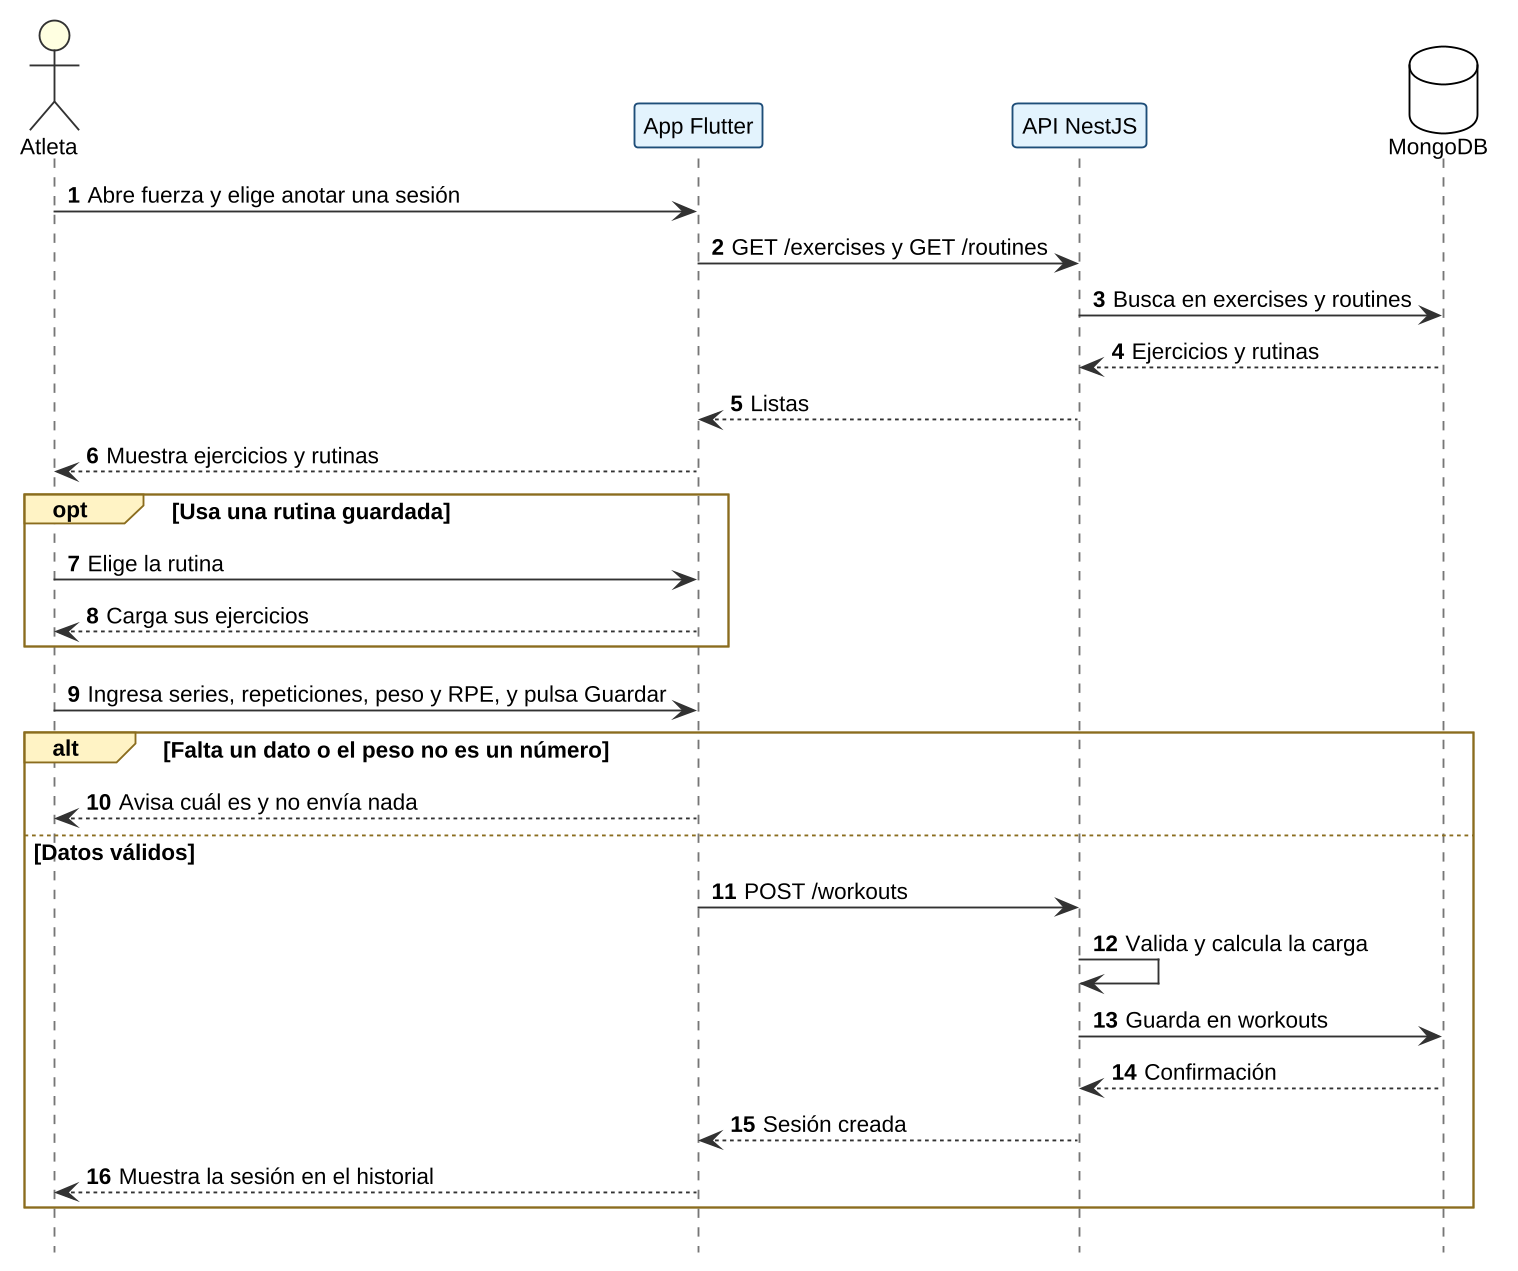
\includegraphics[width=0.95\textwidth,height=0.6\textheight,keepaspectratio]{figuras/secuencia/sec_cu01.png}
    \captionof{figure}{Diagrama de Secuencia -- CU-01: Anotar una sesión de fuerza.}
    \label{fig:sec_cu01}
\end{center}
La aplicación carga el catálogo de ejercicios y las rutinas del usuario. Cuando este pulsa Guardar, la propia aplicación revisa que no falten datos antes de enviarlos. El backend vuelve a validarlos, calcula la carga de la sesión y la guarda en \texttt{workouts}.
\end{minipage}
\vspace{0.6cm}

\noindent\begin{minipage}{\linewidth}
\textbf{CU-02. Contar mi sesión de fuerza con mis palabras}

Para el caso de uso CU-02 se genera el diagrama de secuencia que se muestra en la Figura \ref{fig:sec_cu02}.
\begin{center}
    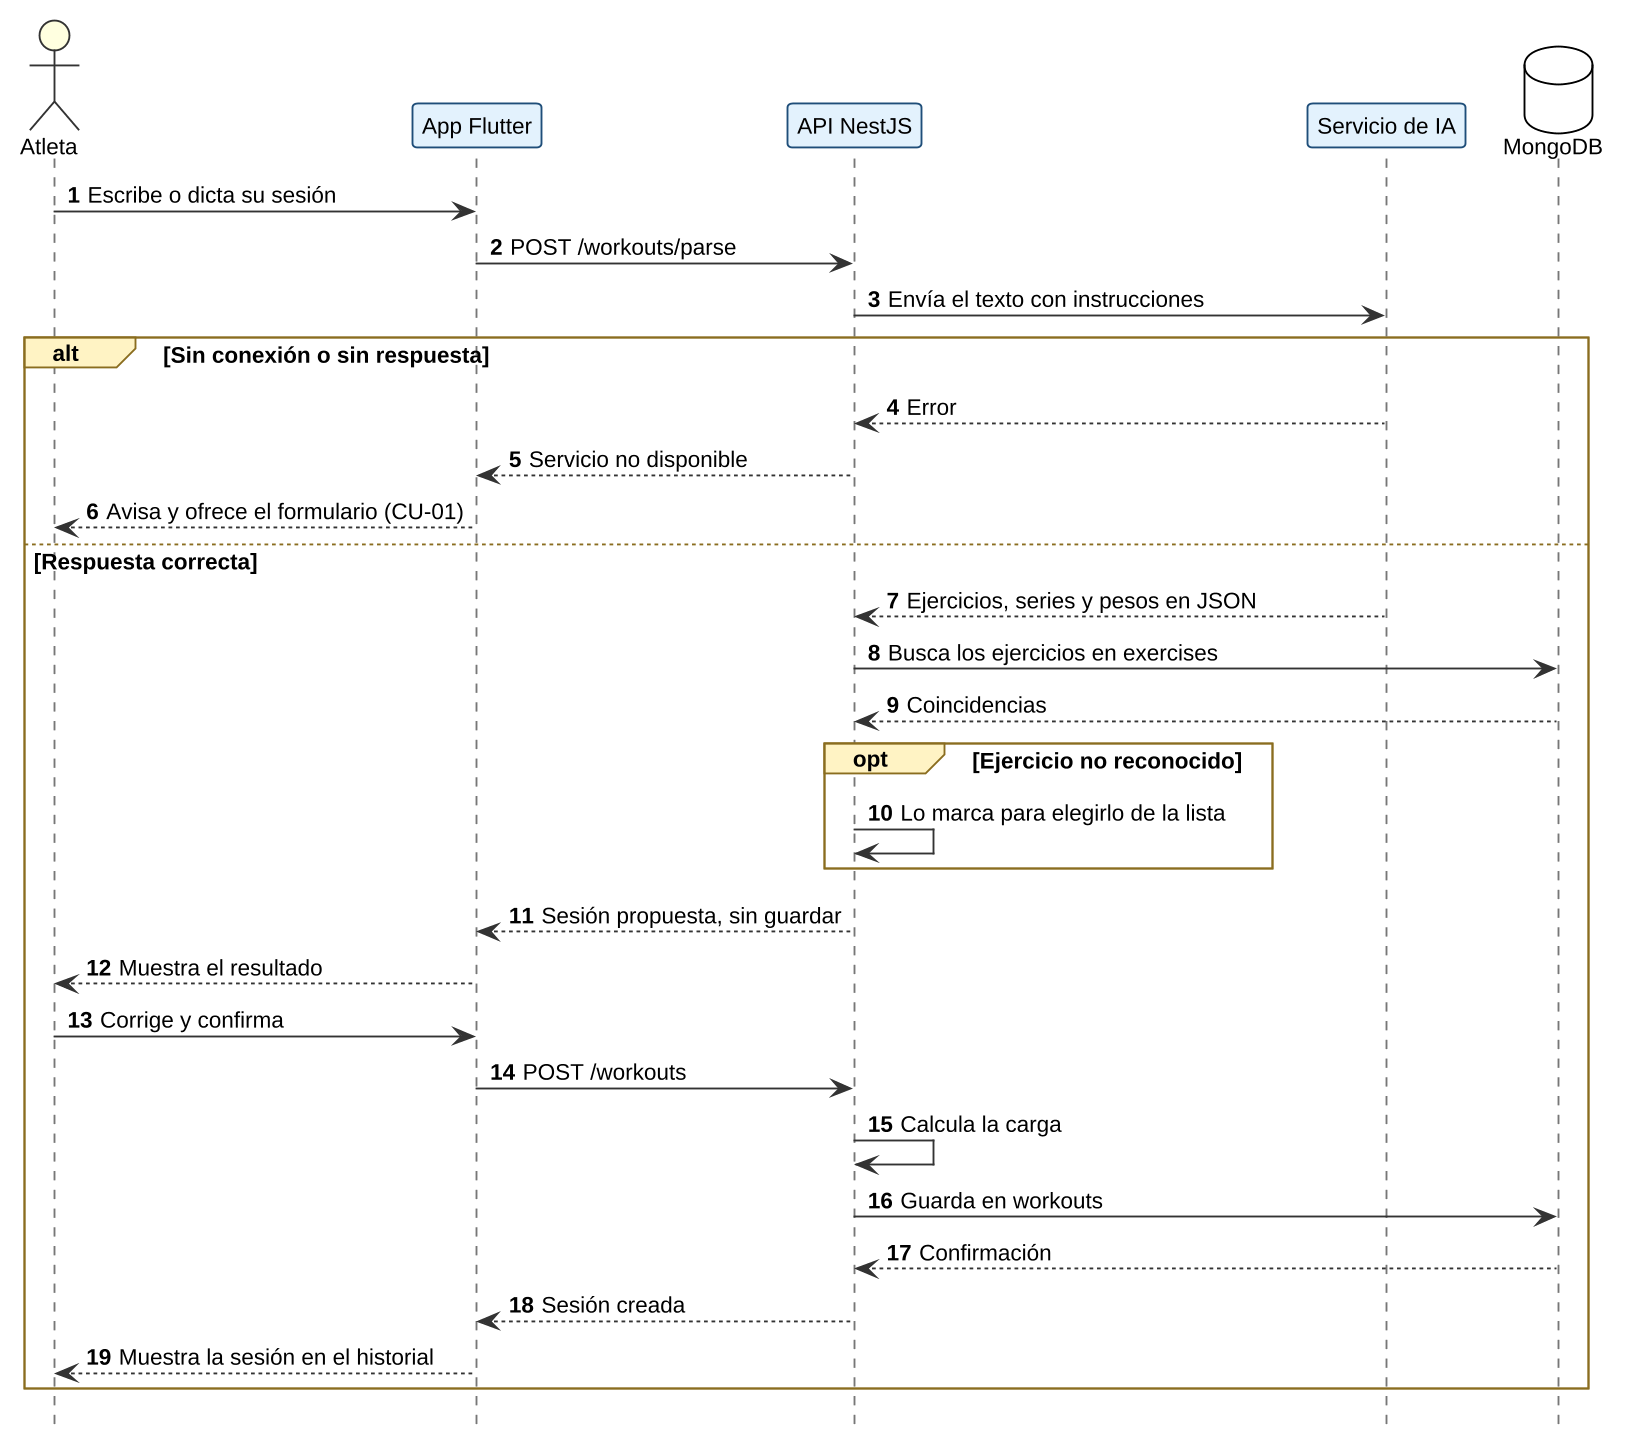
\includegraphics[width=0.95\textwidth,height=0.6\textheight,keepaspectratio]{figuras/secuencia/sec_cu02.png}
    \captionof{figure}{Diagrama de Secuencia -- CU-02: Contar mi sesión de fuerza con mis palabras.}
    \label{fig:sec_cu02}
\end{center}
La aplicación envía el texto al backend, y este lo reenvía al servicio de IA con instrucciones predefinidas para recibir la sesión ordenada en JSON. Luego compara cada ejercicio con el catálogo. La sesión solo se guarda cuando el usuario la confirma. Si el servicio de IA falla, se ofrece el formulario del CU-01.
\end{minipage}
\vspace{0.6cm}

\noindent\begin{minipage}{\linewidth}
\textbf{CU-03. Traer mis sesiones desde el reloj}

Para el caso de uso CU-03 se genera el diagrama de secuencia que se muestra en la Figura \ref{fig:sec_cu03}.
\begin{center}
    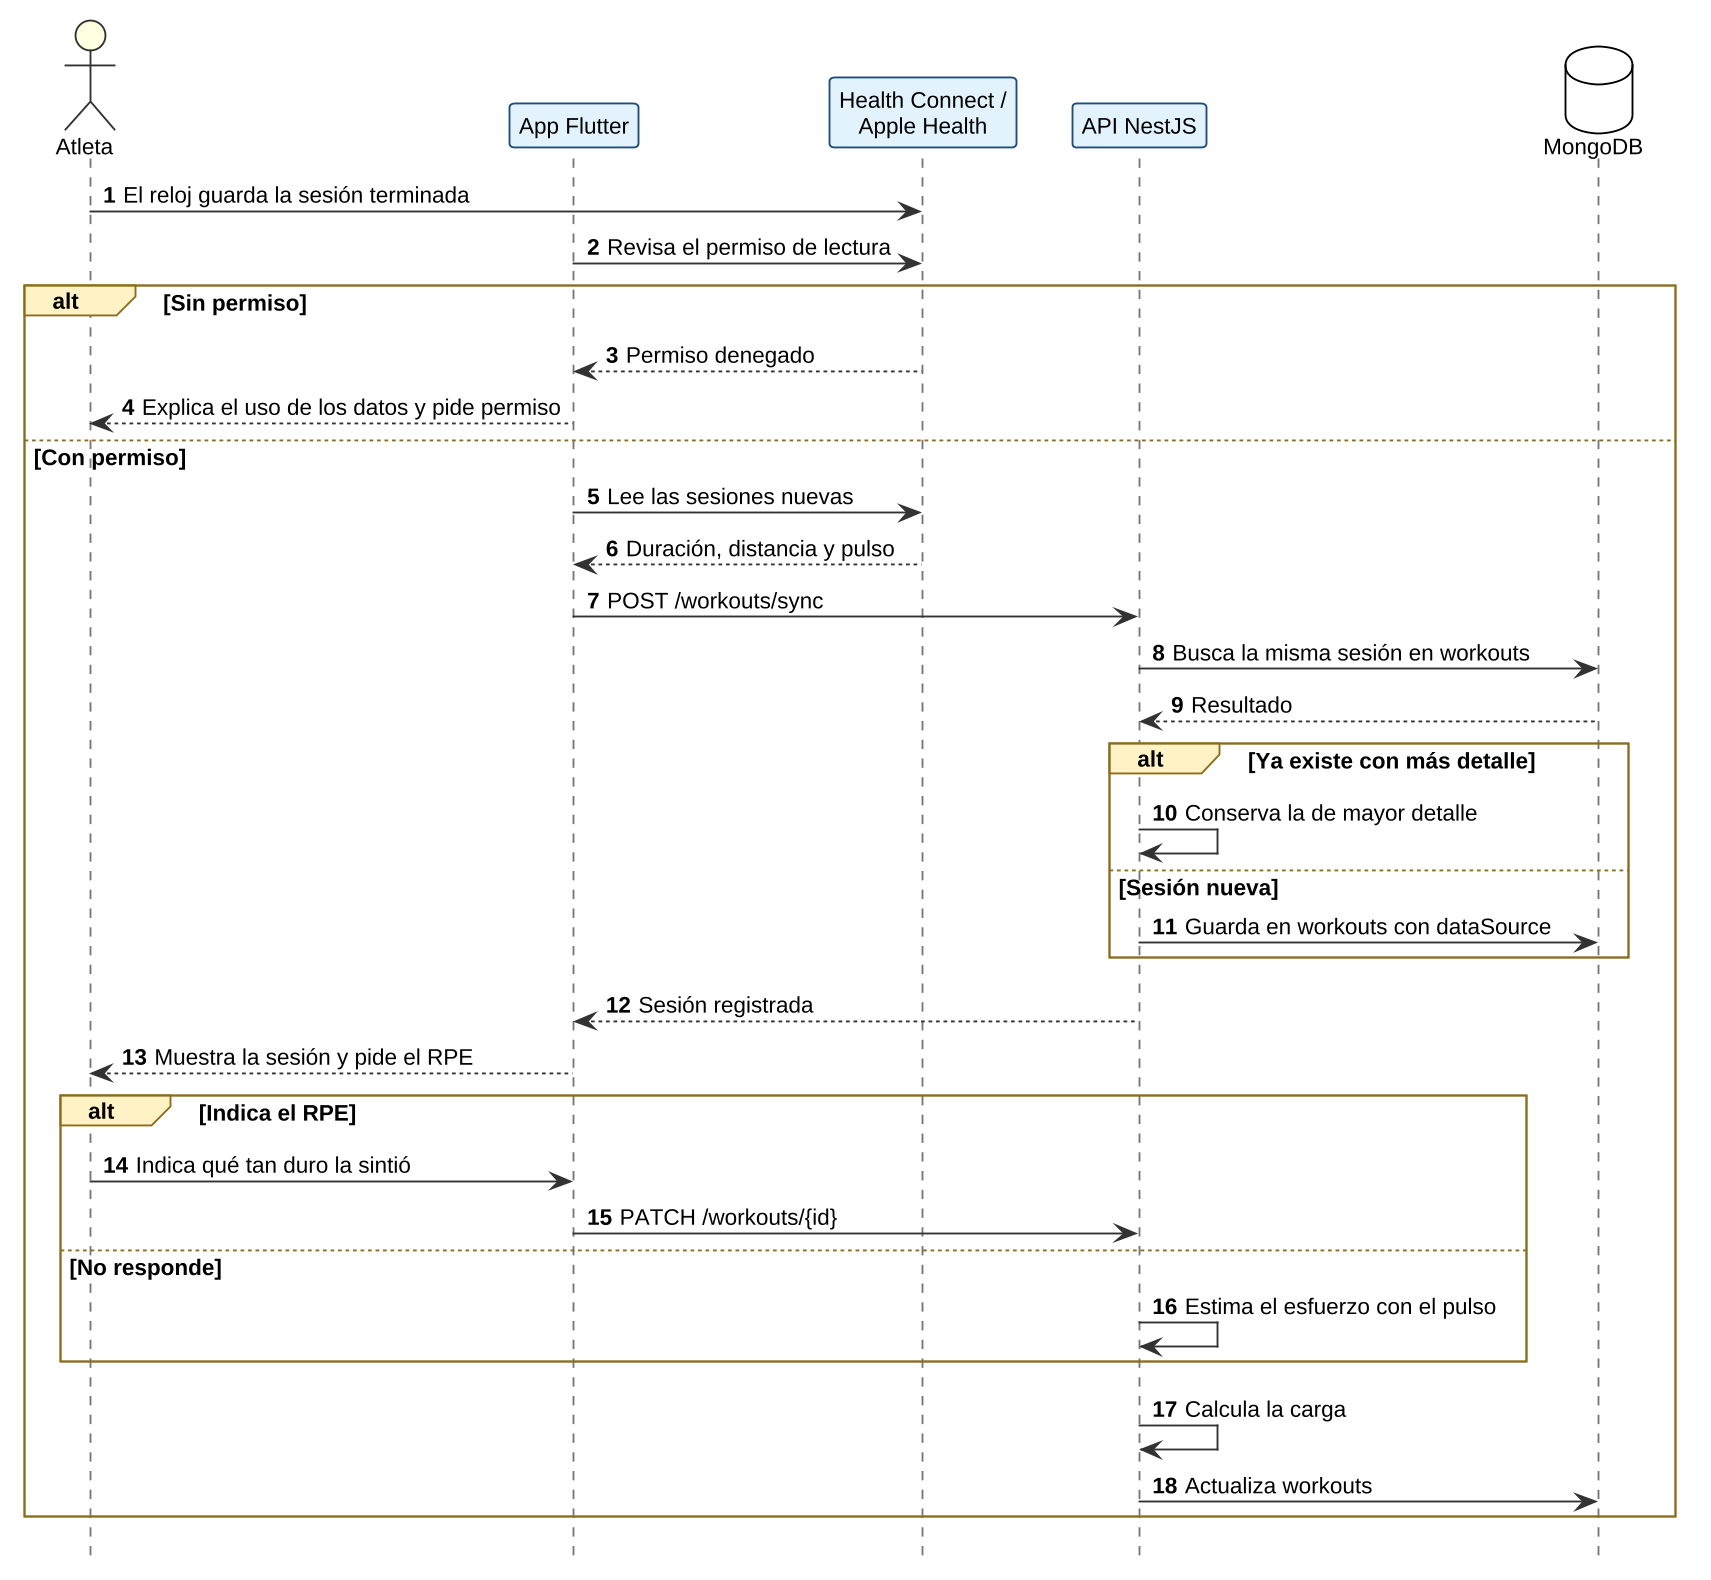
\includegraphics[width=0.95\textwidth,height=0.6\textheight,keepaspectratio]{figuras/secuencia/sec_cu03.png}
    \captionof{figure}{Diagrama de Secuencia -- CU-03: Traer mis sesiones desde el reloj.}
    \label{fig:sec_cu03}
\end{center}
La lectura la hace la aplicación en el teléfono, porque Health Connect y Apple Health no están disponibles desde el servidor. Con el permiso del usuario, lee las sesiones nuevas y las envía al backend. Este revisa que la misma sesión no exista ya con más detalle y luego la guarda. Si el usuario no indica su RPE, el esfuerzo se estima con el pulso.
\end{minipage}
\vspace{0.6cm}

\noindent\begin{minipage}{\linewidth}
\textbf{CU-04. Subir el archivo de mi ciclocomputador}

Para el caso de uso CU-04 se genera el diagrama de secuencia que se muestra en la Figura \ref{fig:sec_cu04}.
\begin{center}
    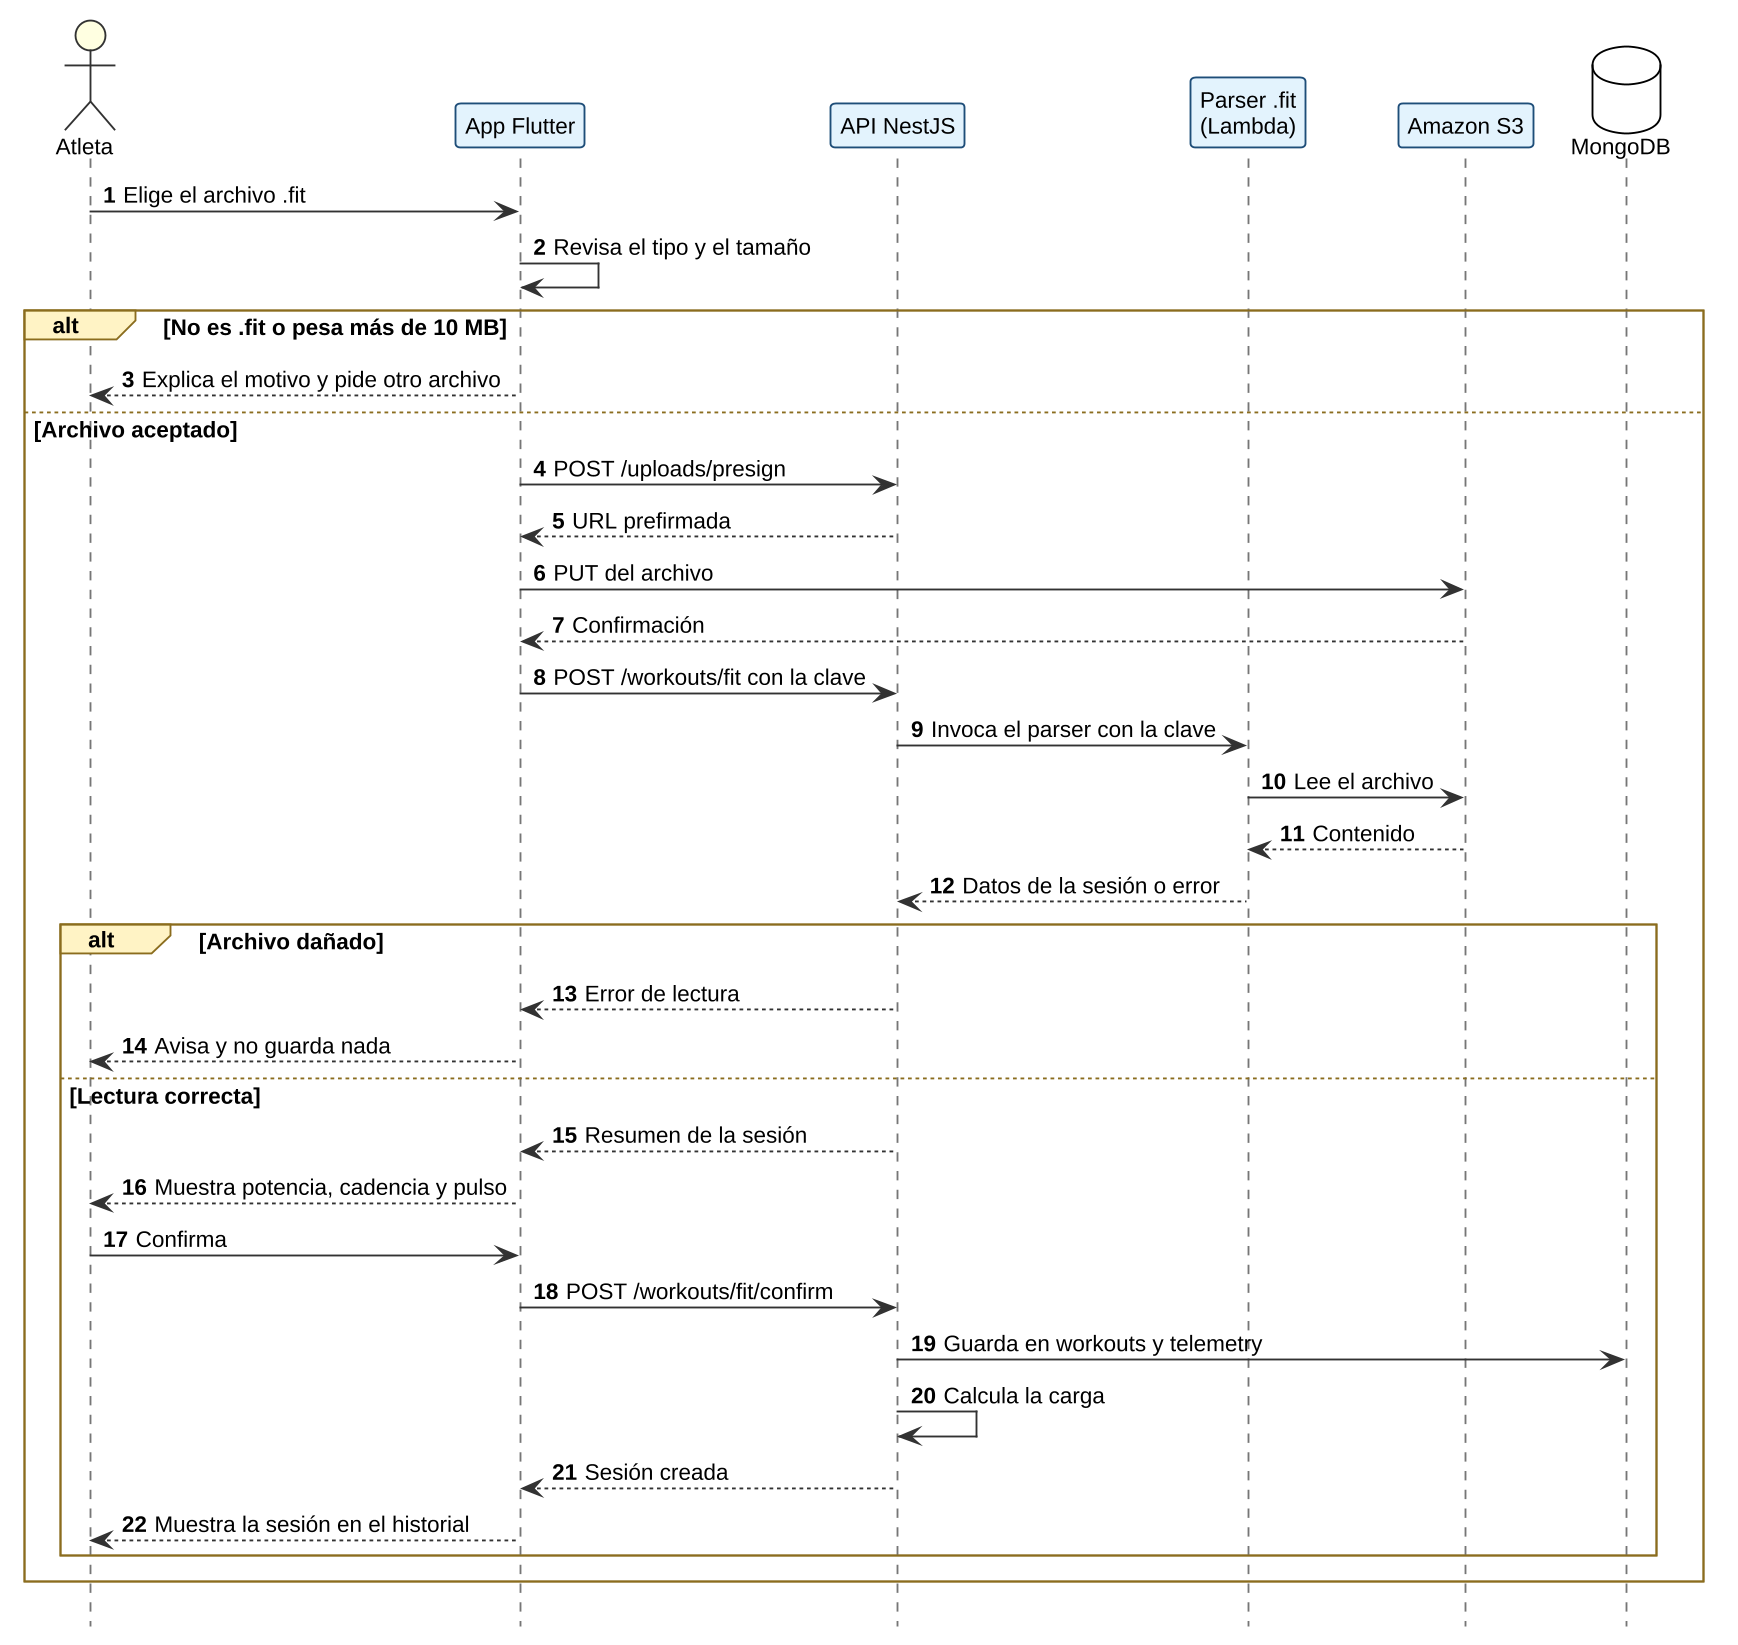
\includegraphics[width=0.95\textwidth,height=0.6\textheight,keepaspectratio]{figuras/secuencia/sec_cu04.png}
    \captionof{figure}{Diagrama de Secuencia -- CU-04: Subir el archivo de mi ciclocomputador.}
    \label{fig:sec_cu04}
\end{center}
El archivo se sube directamente a Amazon S3 con una URL prefirmada, para que el backend no reciba archivos pesados. Luego el backend invoca una función Lambda, que lee el archivo con el parser y devuelve un resumen. Al confirmar el usuario, guarda la sesión en \texttt{workouts} y los datos segundo a segundo en \texttt{telemetry}. Si el archivo está dañado no se guarda ningún dato, y el archivo en S3 se borra con la regla automática del bucket.
\end{minipage}
\vspace{0.6cm}

\noindent\begin{minipage}{\linewidth}
\textbf{CU-05. Revisar mi fatiga y recibir alertas}

Para el caso de uso CU-05 se genera el diagrama de secuencia que se muestra en la Figura \ref{fig:sec_cu05}.
\begin{center}
    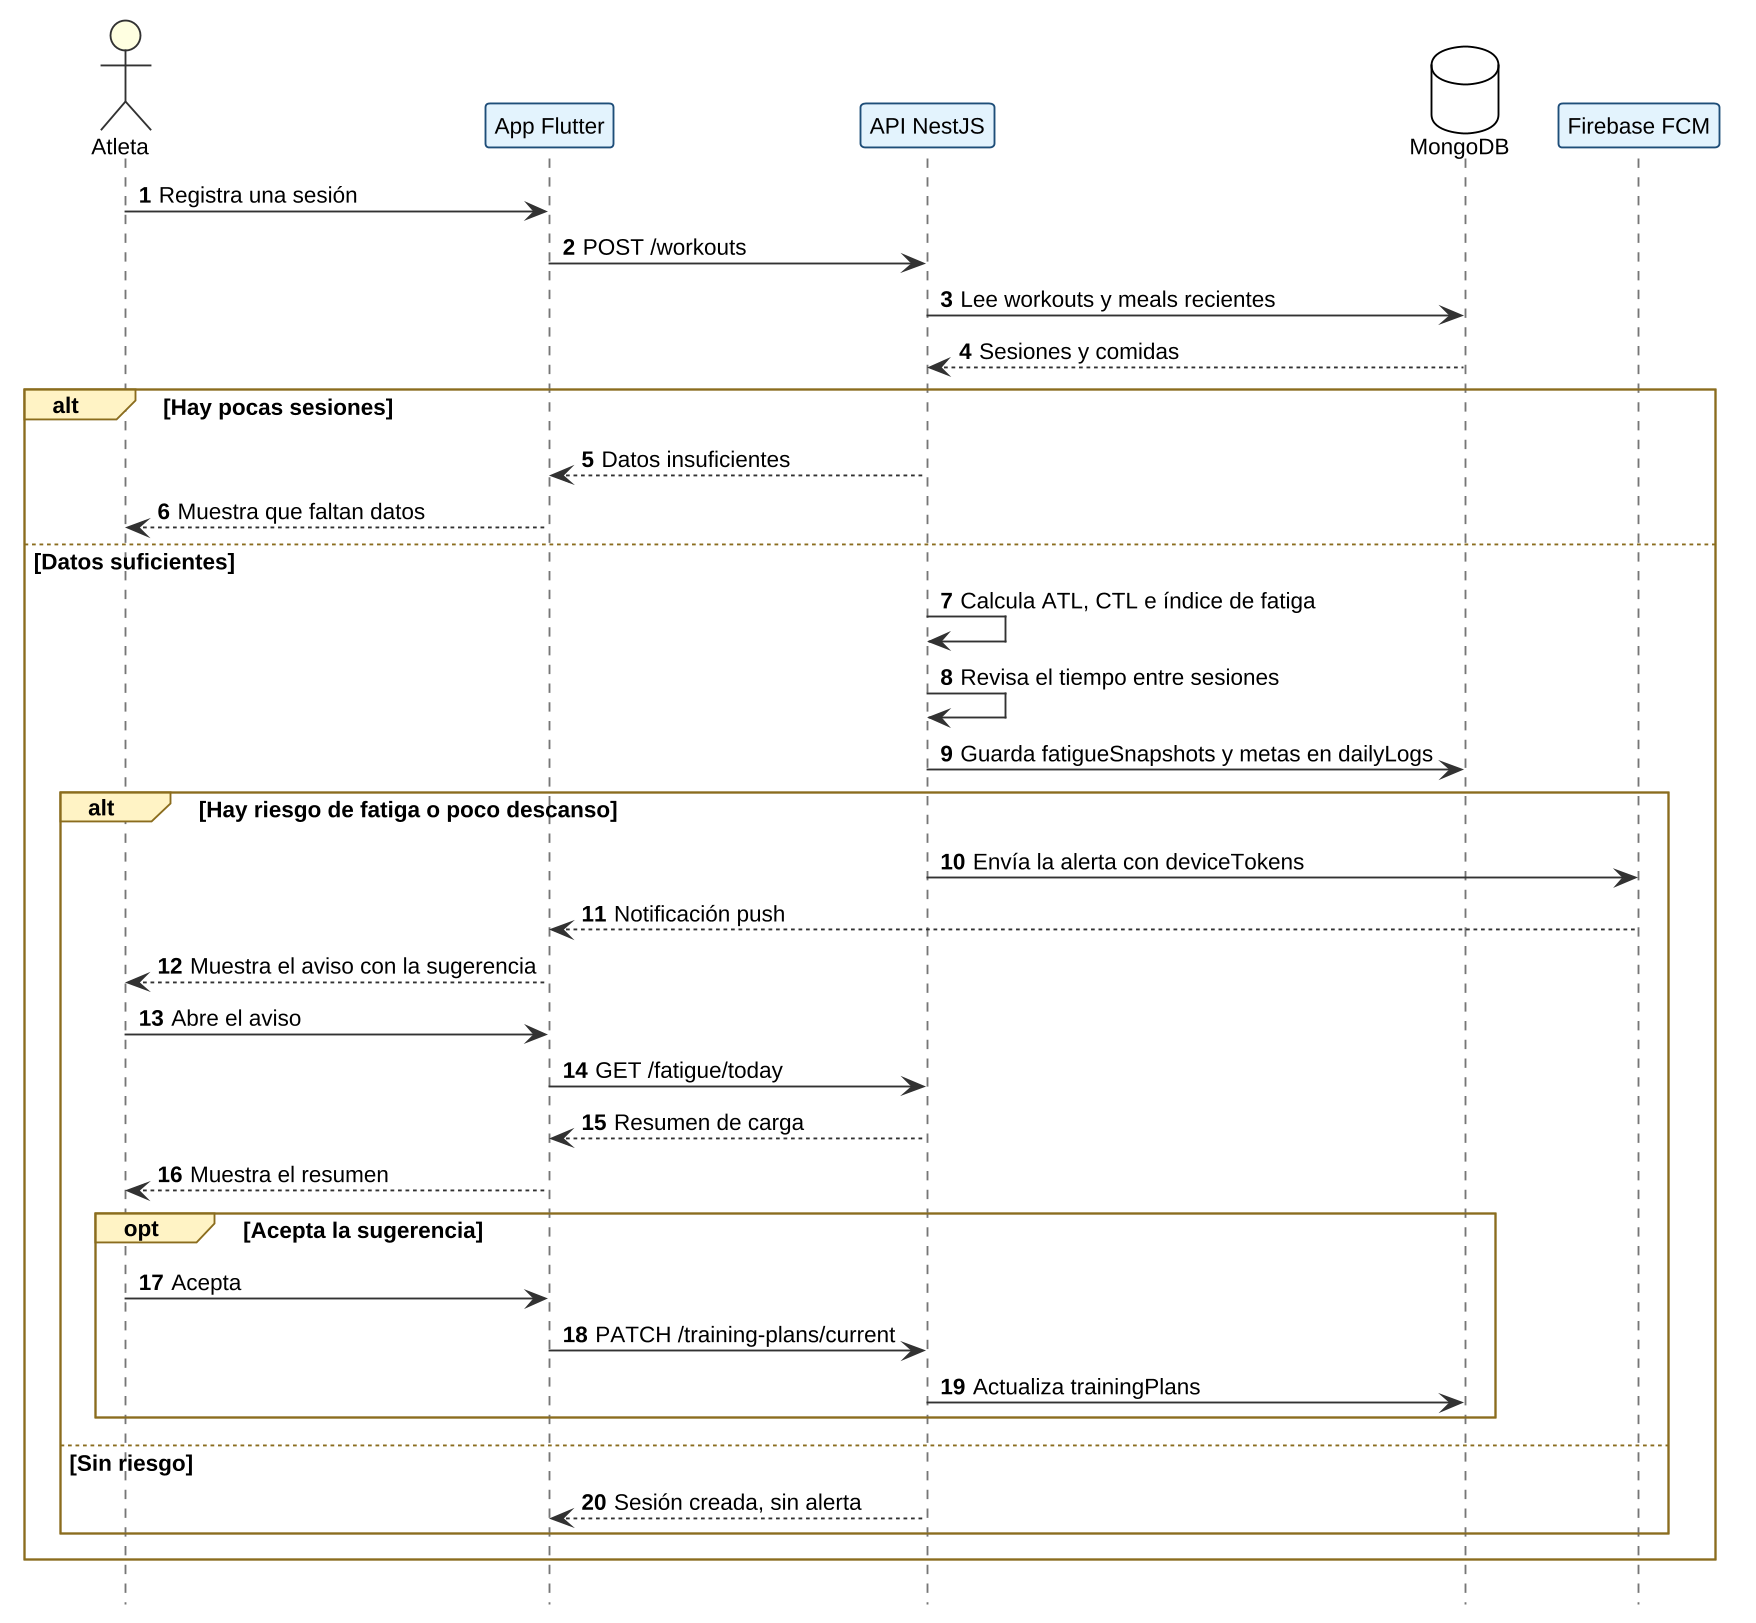
\includegraphics[width=0.95\textwidth,height=0.6\textheight,keepaspectratio]{figuras/secuencia/sec_cu05.png}
    \captionof{figure}{Diagrama de Secuencia -- CU-05: Revisar mi fatiga y recibir alertas.}
    \label{fig:sec_cu05}
\end{center}
El cálculo se hace después de cada sesión. El backend lee las sesiones y comidas recientes, calcula las cargas ATL y CTL, el índice de fatiga y el tiempo entre sesiones, y guarda el resultado en \texttt{fatigueSnapshots}. También actualiza las metas del día. Si detecta un riesgo, envía la alerta por Firebase Cloud Messaging. El plan solo cambia si el usuario acepta la sugerencia.
\end{minipage}
\vspace{0.6cm}

\noindent\begin{minipage}{\linewidth}
\textbf{CU-06. Anotar una comida buscando los alimentos}

Para el caso de uso CU-06 se genera el diagrama de secuencia que se muestra en la Figura \ref{fig:sec_cu06}.
\begin{center}
    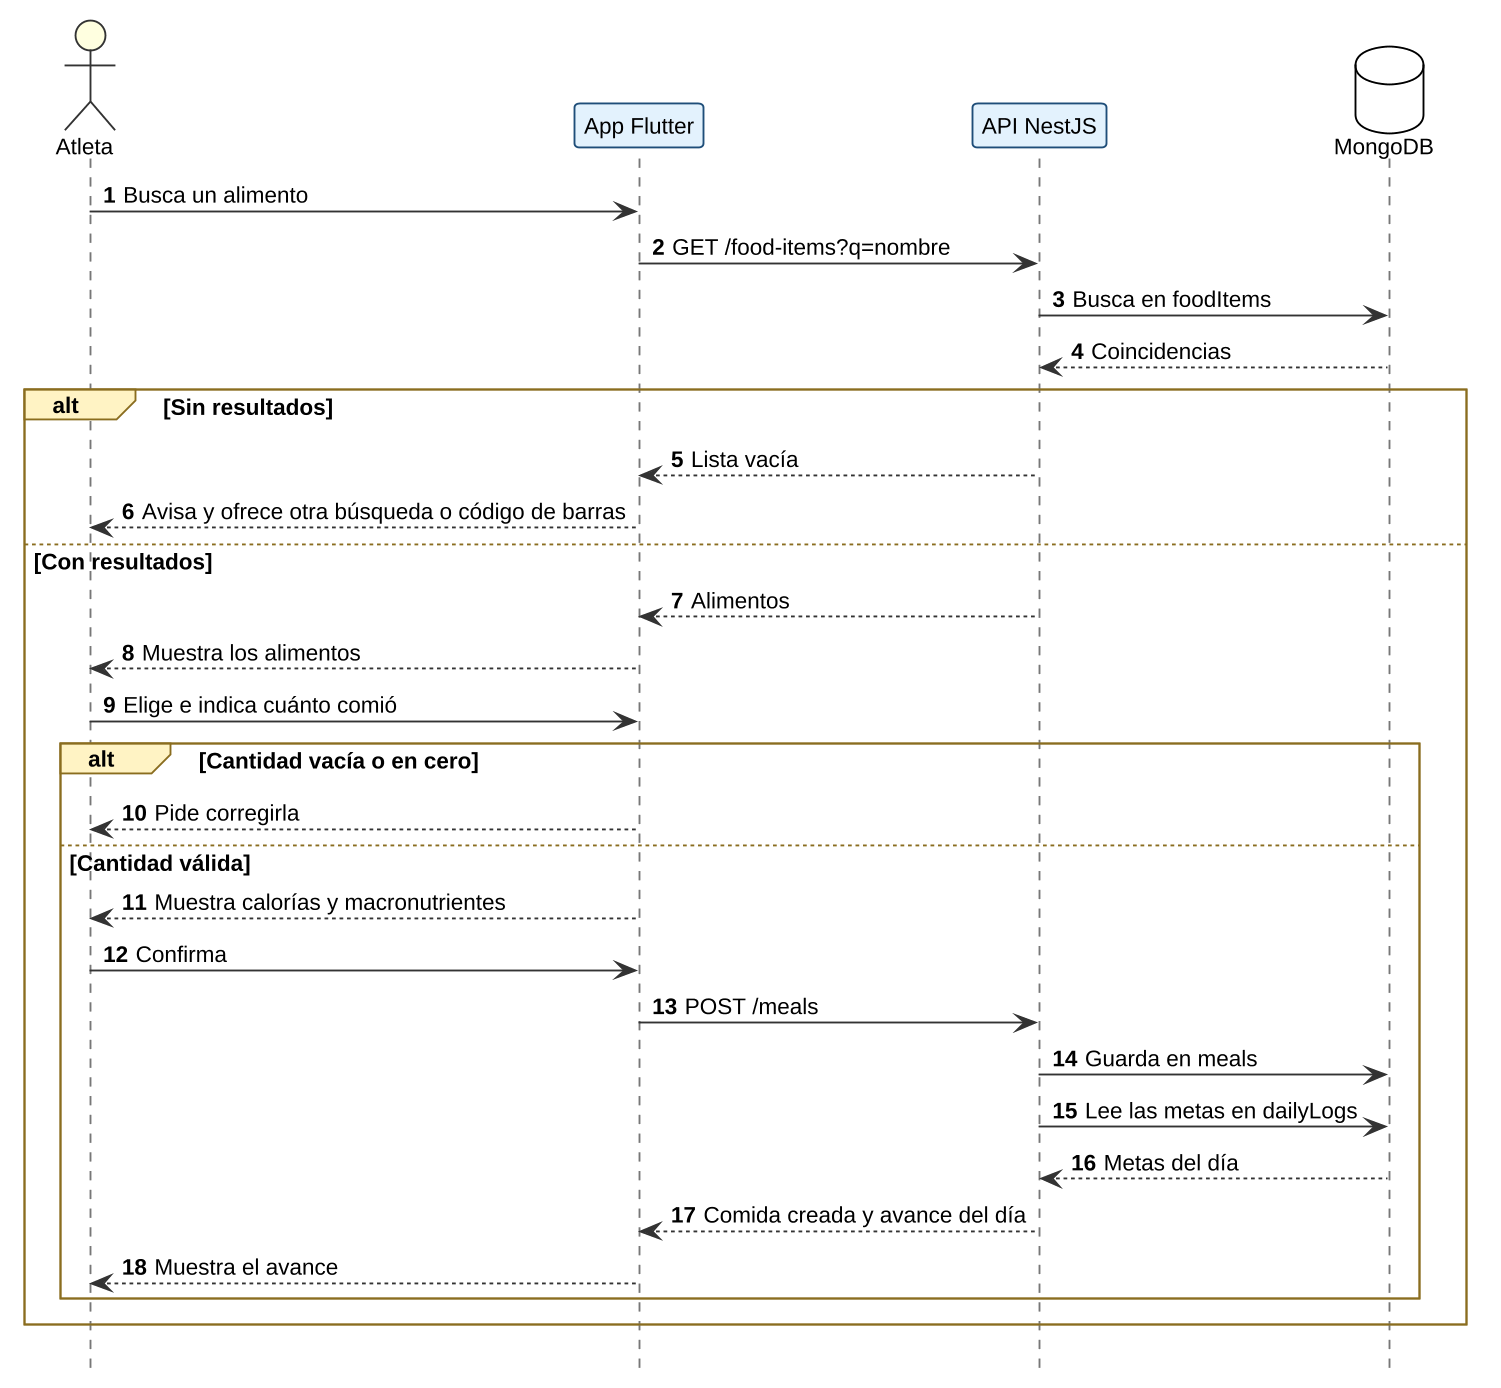
\includegraphics[width=0.95\textwidth,height=0.6\textheight,keepaspectratio]{figuras/secuencia/sec_cu06.png}
    \captionof{figure}{Diagrama de Secuencia -- CU-06: Anotar una comida buscando los alimentos.}
    \label{fig:sec_cu06}
\end{center}
La aplicación busca en el catálogo \texttt{foodItems} a través del backend. Una vez elegido el alimento, revisa la cantidad, muestra los valores y envía la comida. El backend la guarda en \texttt{meals} y responde con el avance respecto a las metas del día.
\end{minipage}
\vspace{0.6cm}

\noindent\begin{minipage}{\linewidth}
\textbf{CU-07. Registrar una comida con una foto}

Para el caso de uso CU-07 se genera el diagrama de secuencia que se muestra en la Figura \ref{fig:sec_cu07}.
\begin{center}
    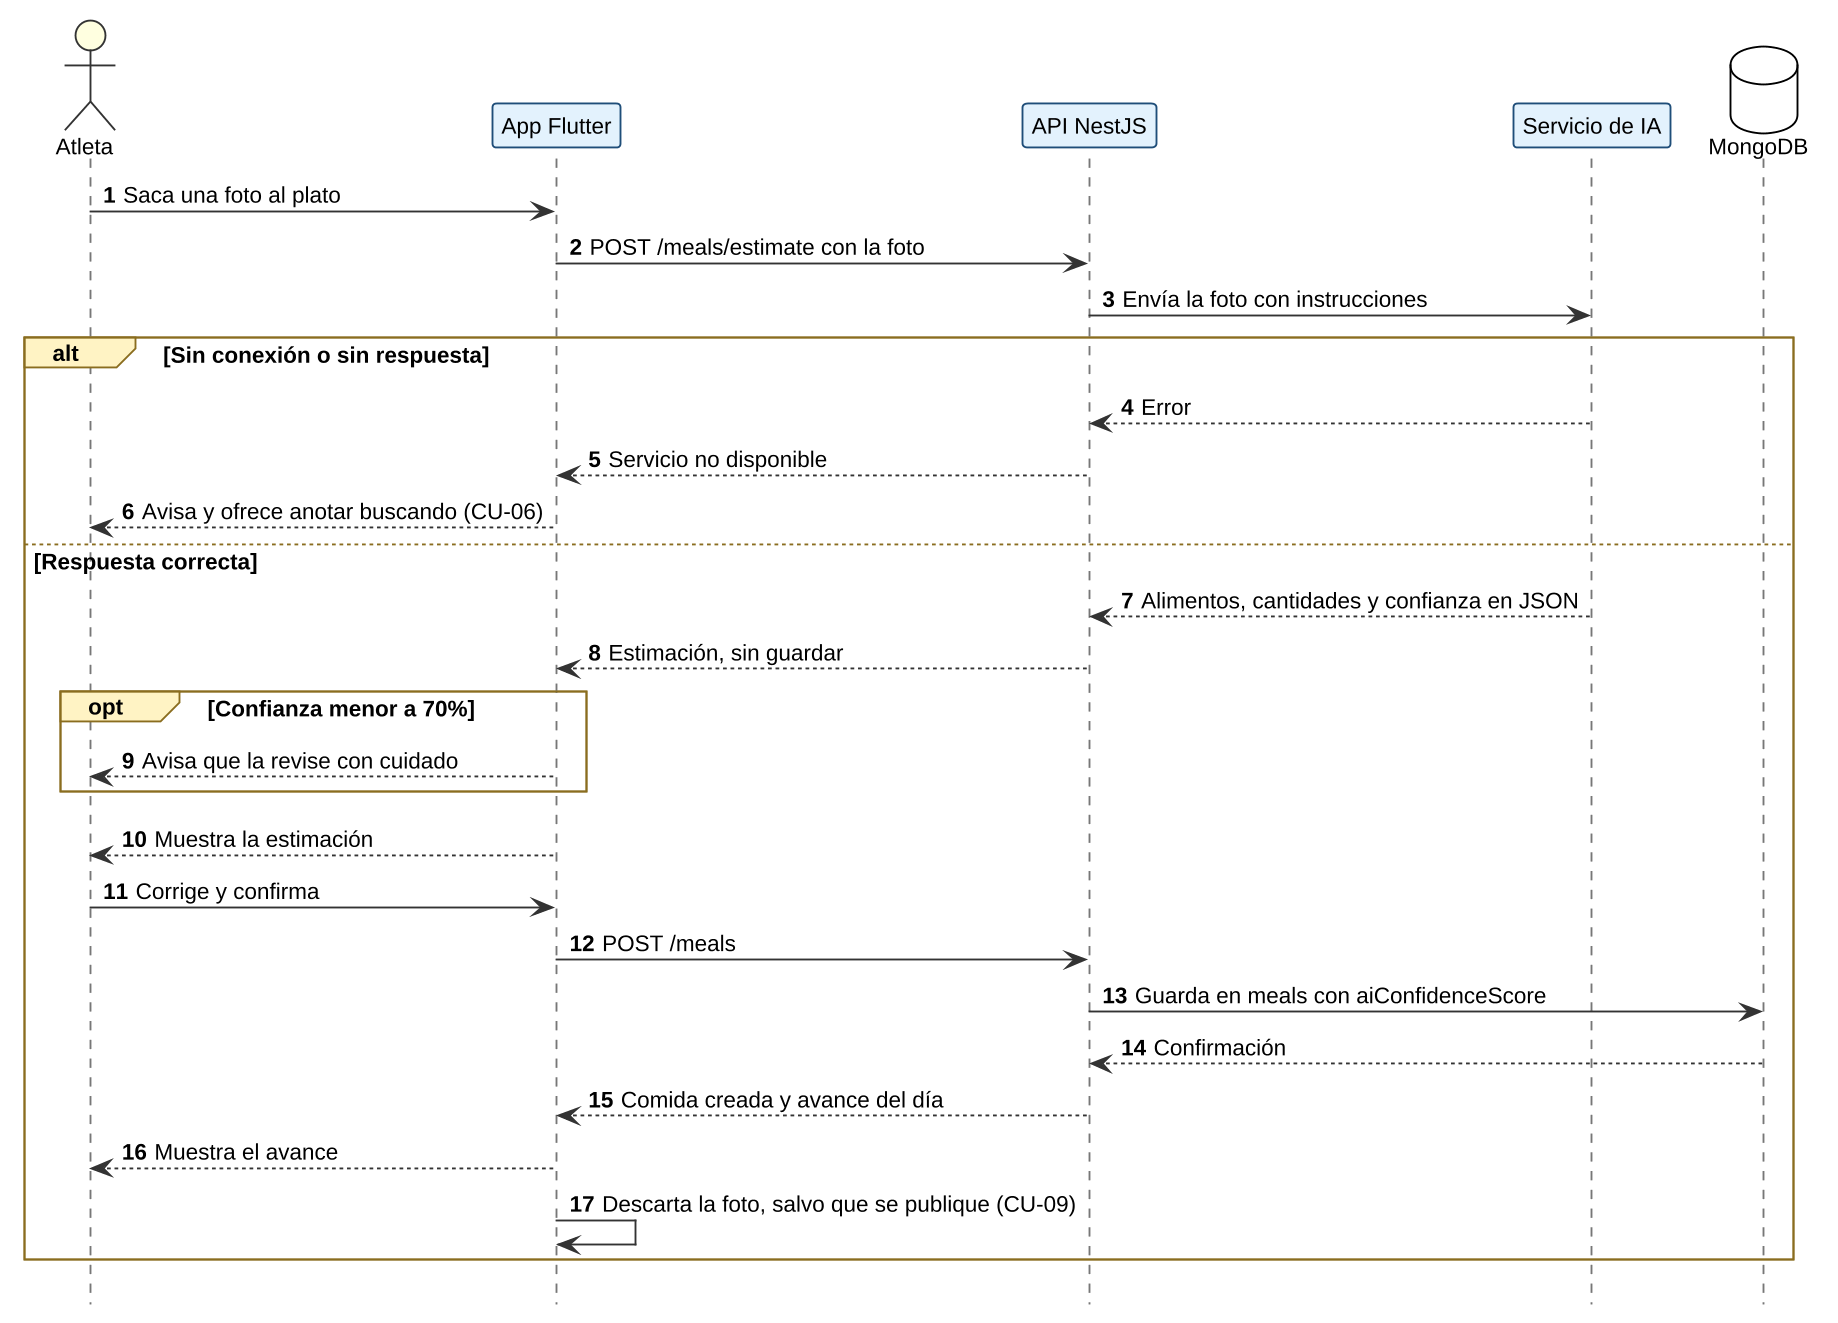
\includegraphics[width=0.95\textwidth,height=0.6\textheight,keepaspectratio]{figuras/secuencia/sec_cu07.png}
    \captionof{figure}{Diagrama de Secuencia -- CU-07: Registrar una comida con una foto.}
    \label{fig:sec_cu07}
\end{center}
La foto se envía al backend y este la reenvía al servicio de IA, sin guardarla en Amazon S3. La respuesta incluye un índice de confianza, y si es menor a 70\% la aplicación pide revisar el resultado con más cuidado. La comida se guarda solo cuando el usuario confirma, junto con ese índice, y la foto se descarta salvo que se publique.
\end{minipage}
\vspace{0.6cm}

\noindent\begin{minipage}{\linewidth}
\textbf{CU-08. Agregar una receta ajustada a mis metas}

Para el caso de uso CU-08 se genera el diagrama de secuencia que se muestra en la Figura \ref{fig:sec_cu08}.
\begin{center}
    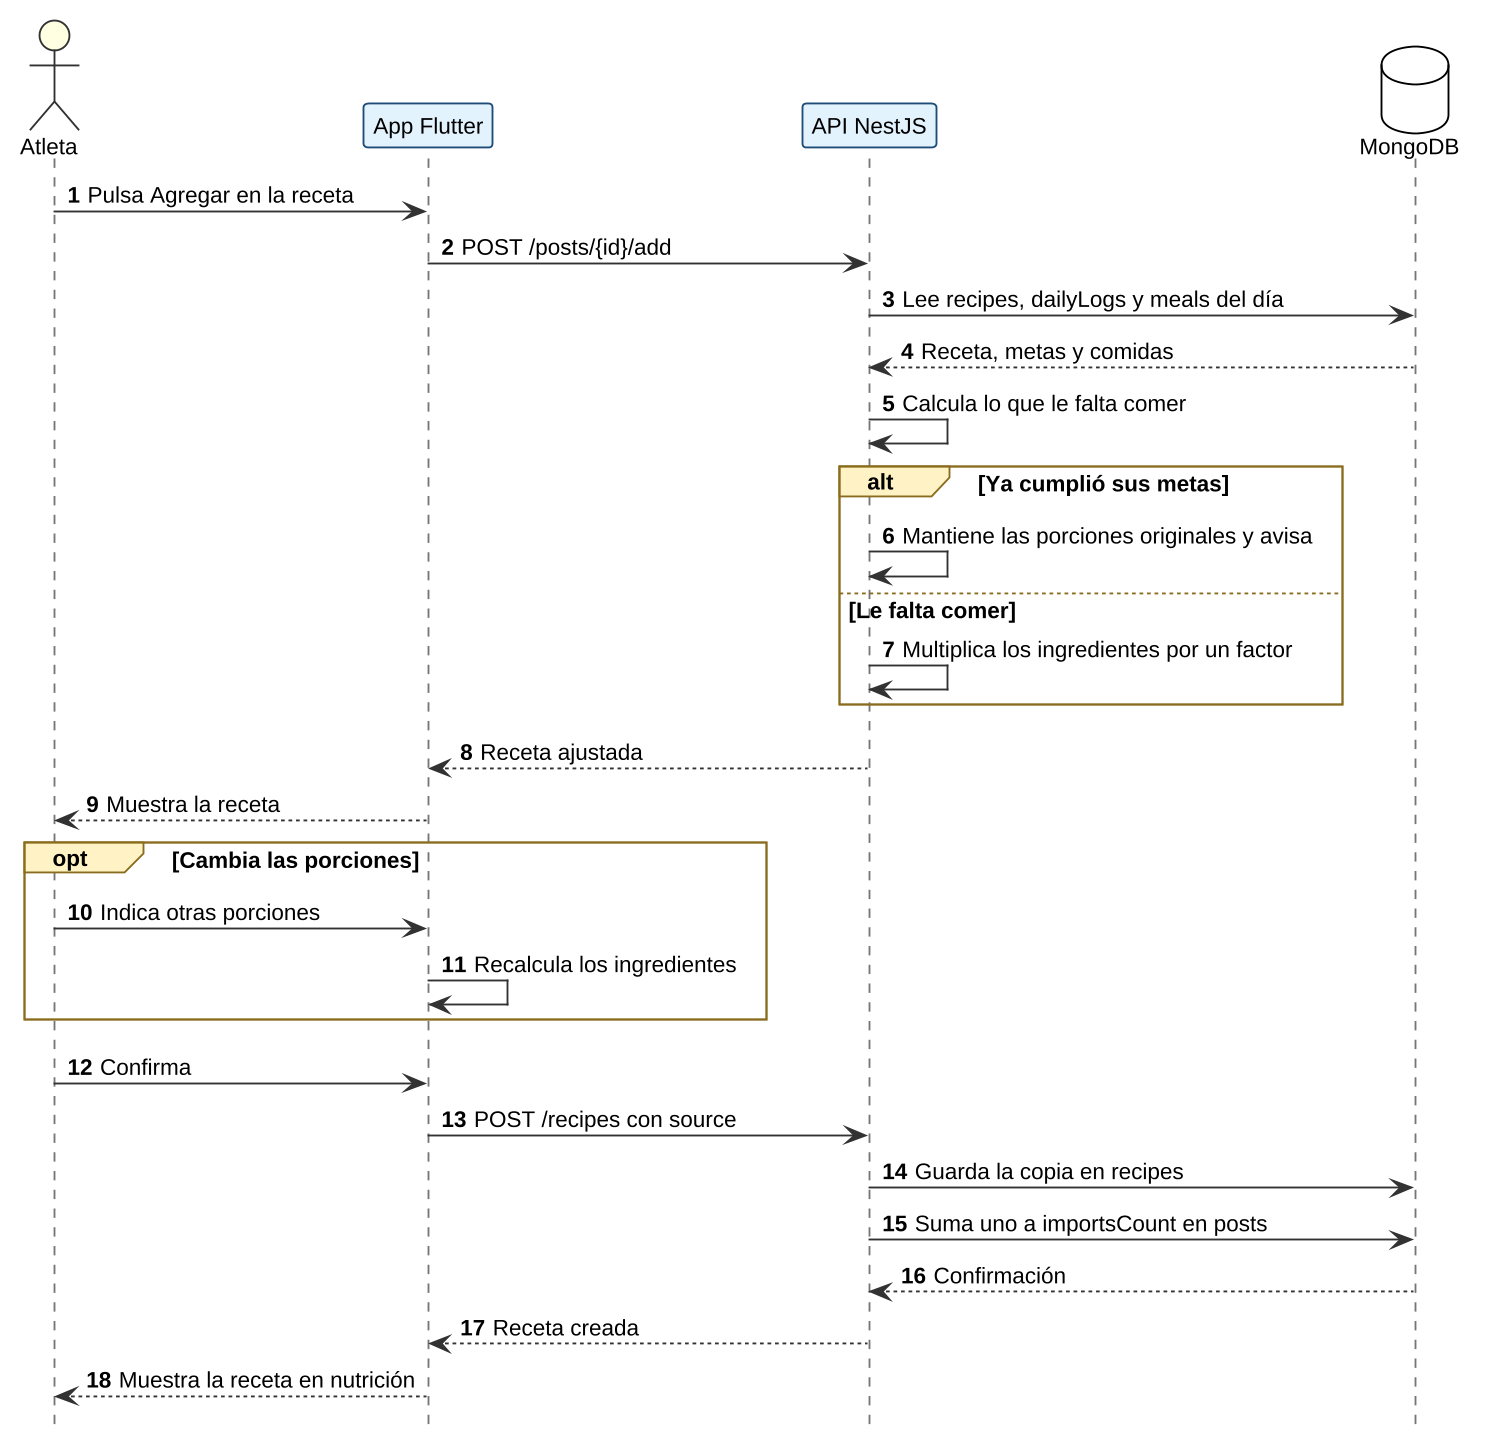
\includegraphics[width=0.95\textwidth,height=0.6\textheight,keepaspectratio]{figuras/secuencia/sec_cu08.png}
    \captionof{figure}{Diagrama de Secuencia -- CU-08: Agregar una receta ajustada a mis metas.}
    \label{fig:sec_cu08}
\end{center}
El backend lee la receta, las metas y las comidas del día para calcular lo que le falta comer al usuario. Con eso obtiene un factor y multiplica todos los ingredientes por él, de modo que las proporciones no cambian. Al confirmar, guarda una copia en \texttt{recipes} con la referencia a su autor y suma uno a \texttt{importsCount}. Agregar la receta no la registra como comida.
\end{minipage}
\vspace{0.6cm}

\noindent\begin{minipage}{\linewidth}
\textbf{CU-09. Publicar una sesión, ruta o comida}

Para el caso de uso CU-09 se genera el diagrama de secuencia que se muestra en la Figura \ref{fig:sec_cu09}.
\begin{center}
    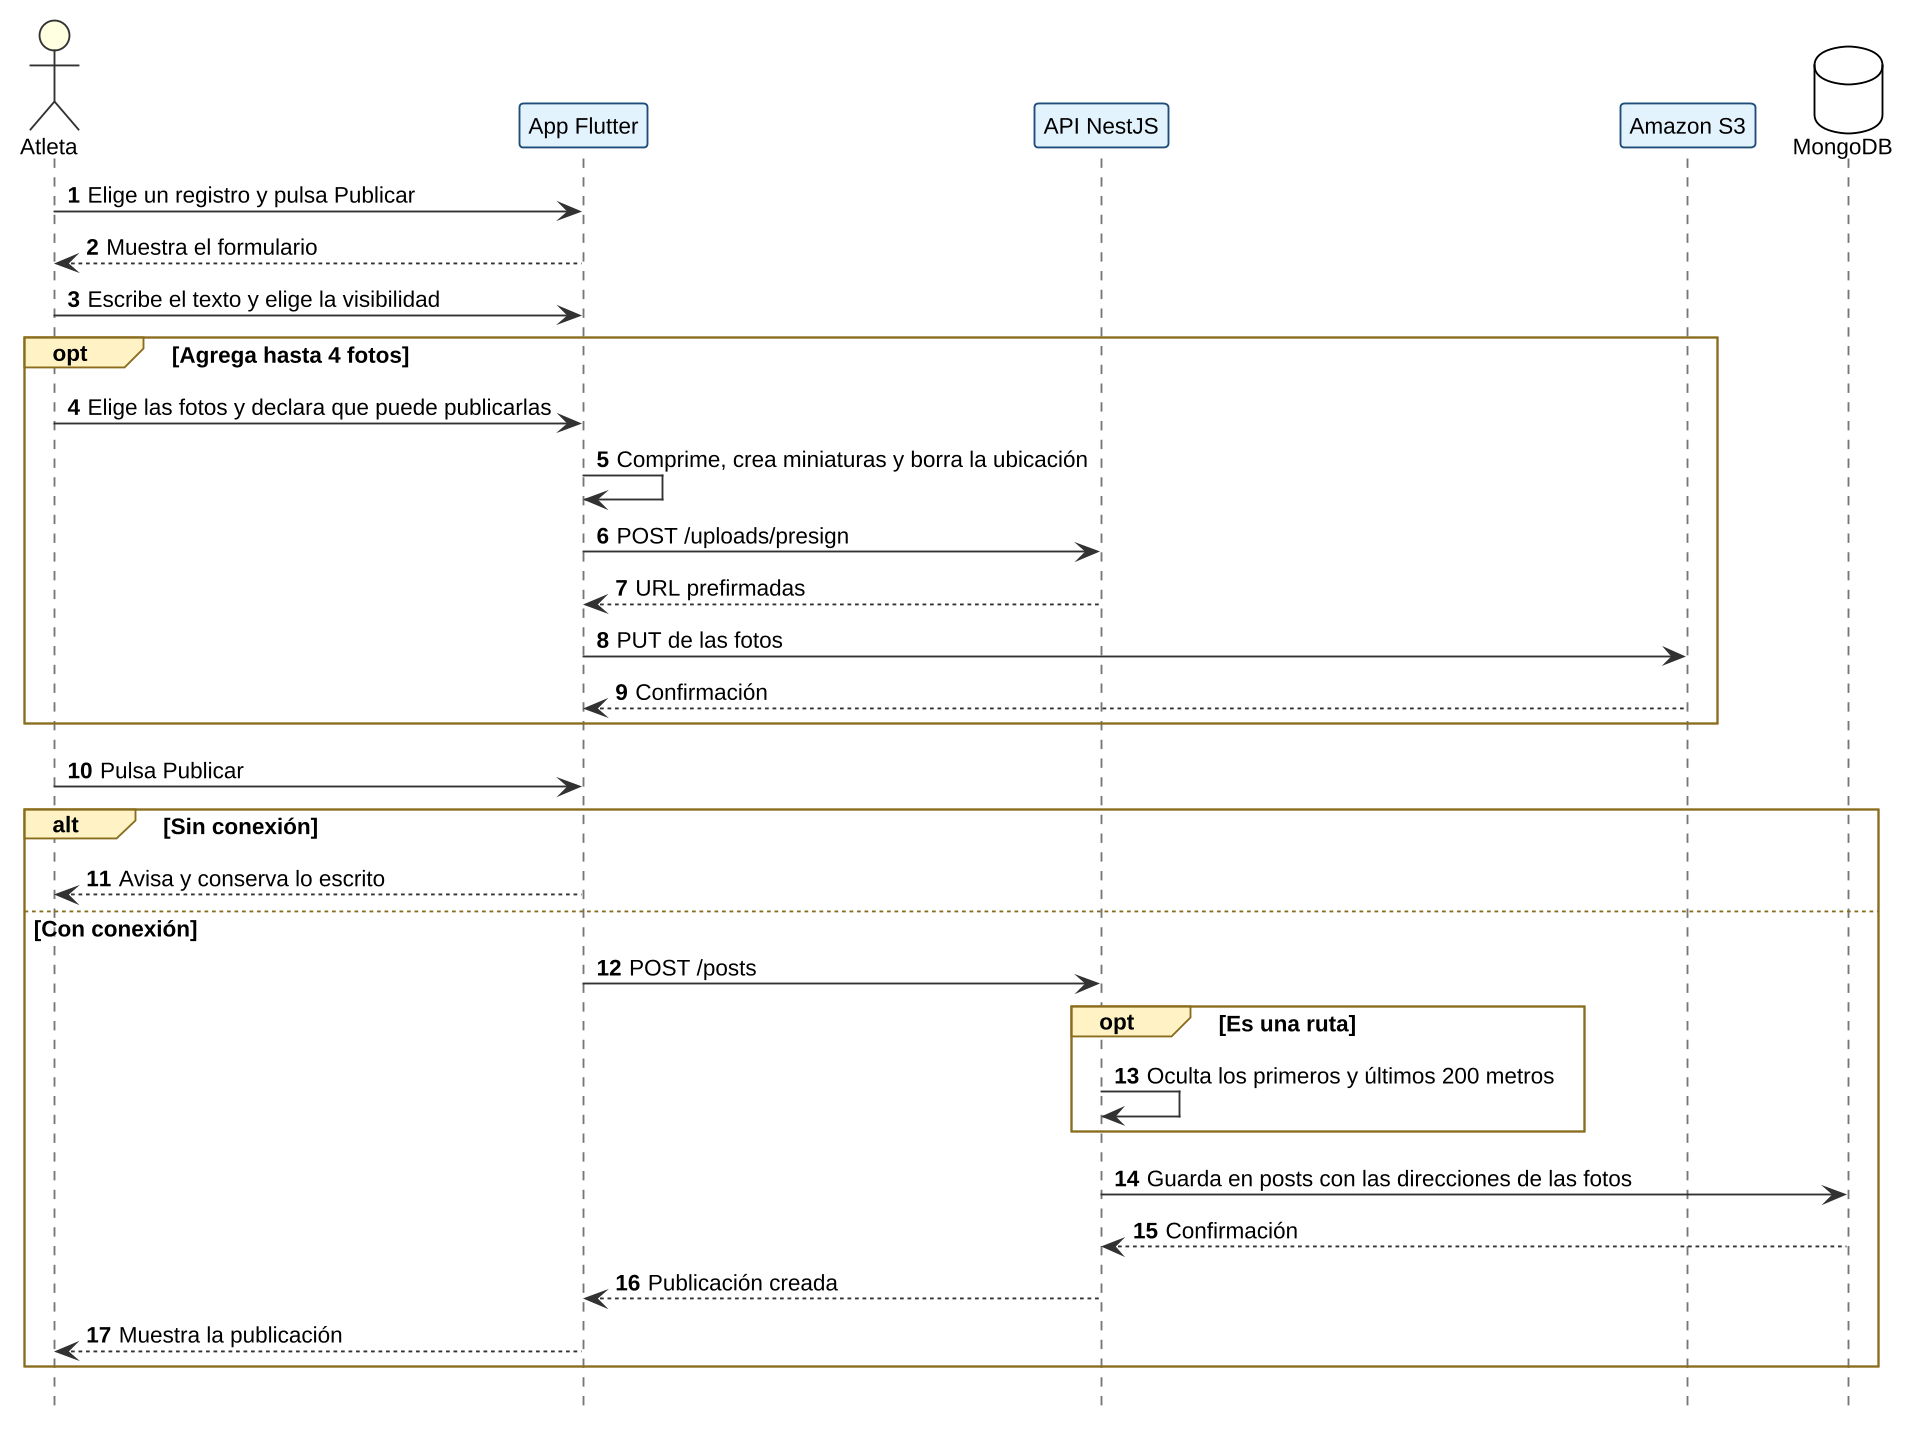
\includegraphics[width=0.95\textwidth,height=0.6\textheight,keepaspectratio]{figuras/secuencia/sec_cu09.png}
    \captionof{figure}{Diagrama de Secuencia -- CU-09: Publicar una sesión, ruta o comida.}
    \label{fig:sec_cu09}
\end{center}
Las fotos se comprimen en el teléfono, donde también se crean las miniaturas y se borra la ubicación. Después se suben directamente a Amazon S3 con URL prefirmadas. El backend guarda la publicación en \texttt{posts} solo con las direcciones de las fotos. Si es una ruta, oculta los primeros y los últimos 200 metros antes de guardarla.
\end{minipage}
\vspace{0.6cm}

\noindent\begin{minipage}{\linewidth}
\textbf{CU-10. Mantener el catálogo de ejercicios}

Para el caso de uso CU-10 se genera el diagrama de secuencia que se muestra en la Figura \ref{fig:sec_cu10}.
\begin{center}
    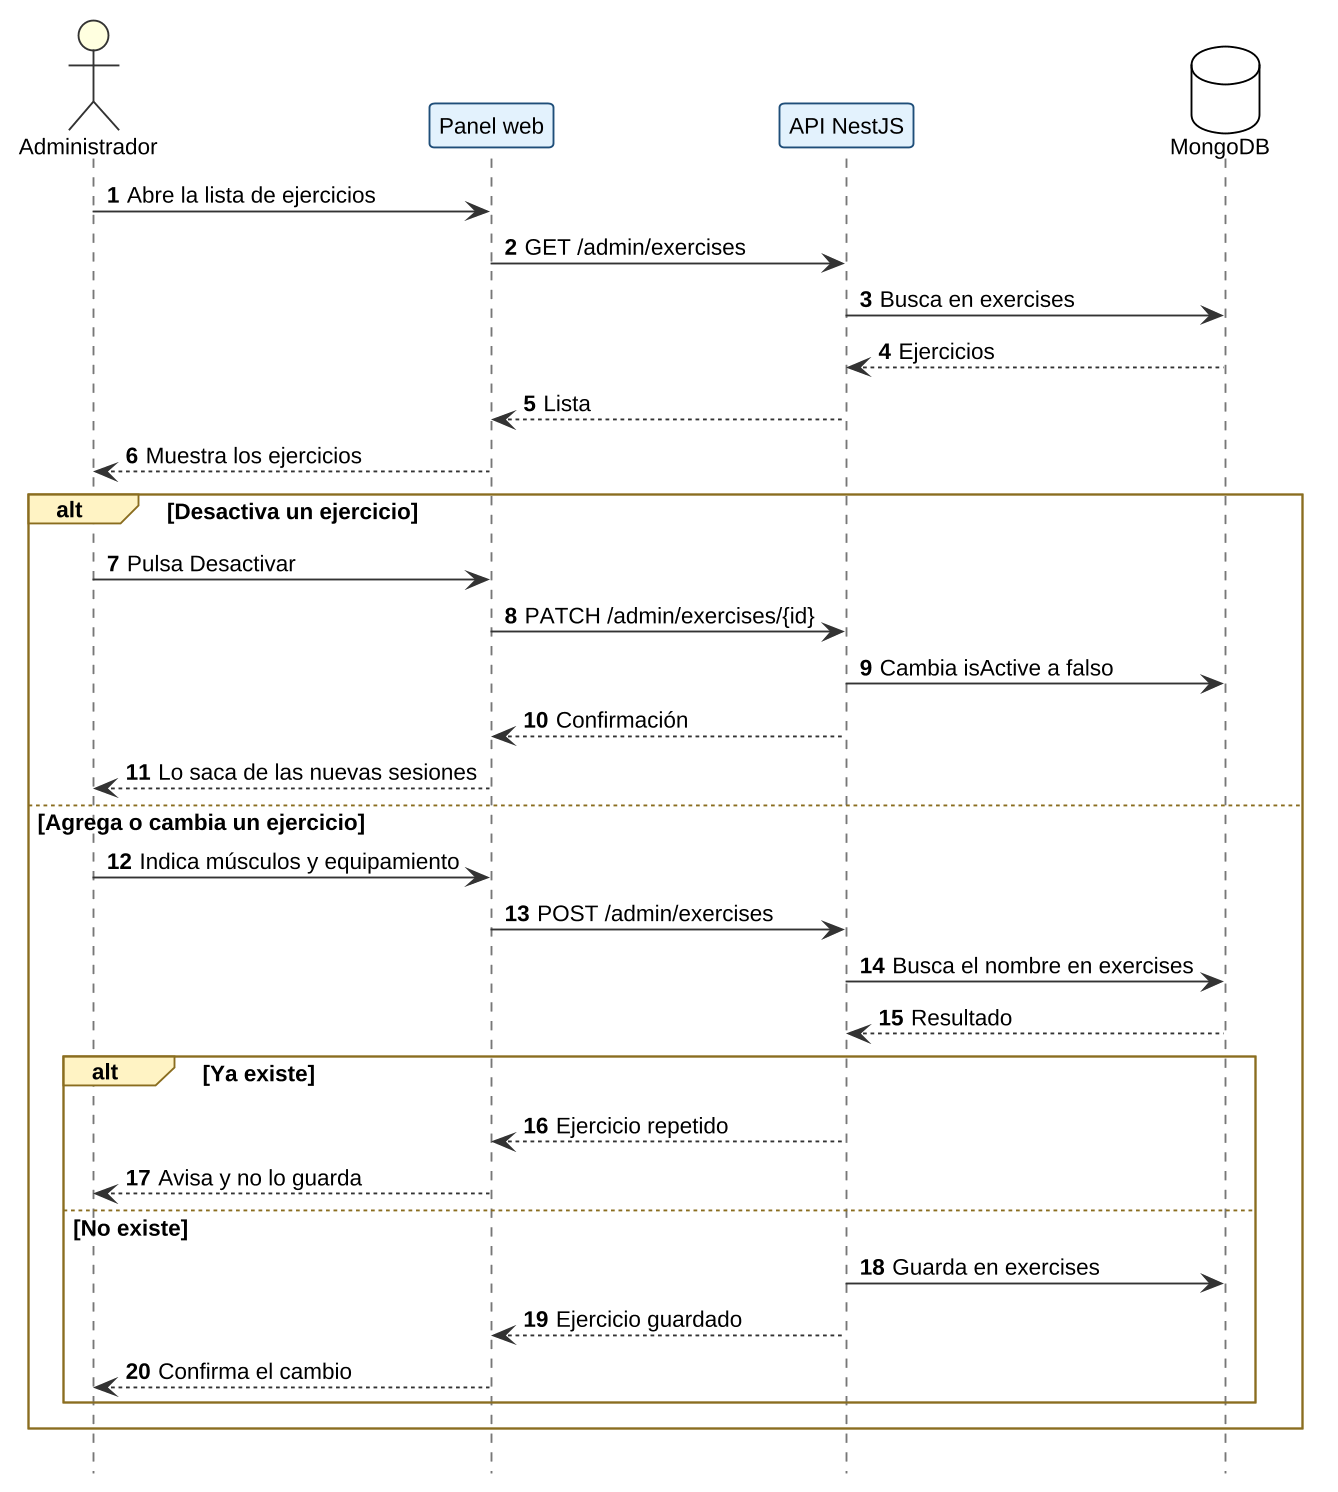
\includegraphics[width=0.95\textwidth,height=0.6\textheight,keepaspectratio]{figuras/secuencia/sec_cu10.png}
    \captionof{figure}{Diagrama de Secuencia -- CU-10: Mantener el catálogo de ejercicios.}
    \label{fig:sec_cu10}
\end{center}
El administrador trabaja desde el panel web, que usa el mismo backend con acceso solo para su rol. Antes de guardar un ejercicio, el backend revisa que el nombre no exista. Los ejercicios no se borran, sino que se desactivan con \texttt{isActive}, para no alterar las sesiones ya registradas.
\end{minipage}
\vspace{0.6cm}

\noindent\begin{minipage}{\linewidth}
\textbf{CU-11. Revisar el contenido reportado}

Para el caso de uso CU-11 se genera el diagrama de secuencia que se muestra en la Figura \ref{fig:sec_cu11}.
\begin{center}
    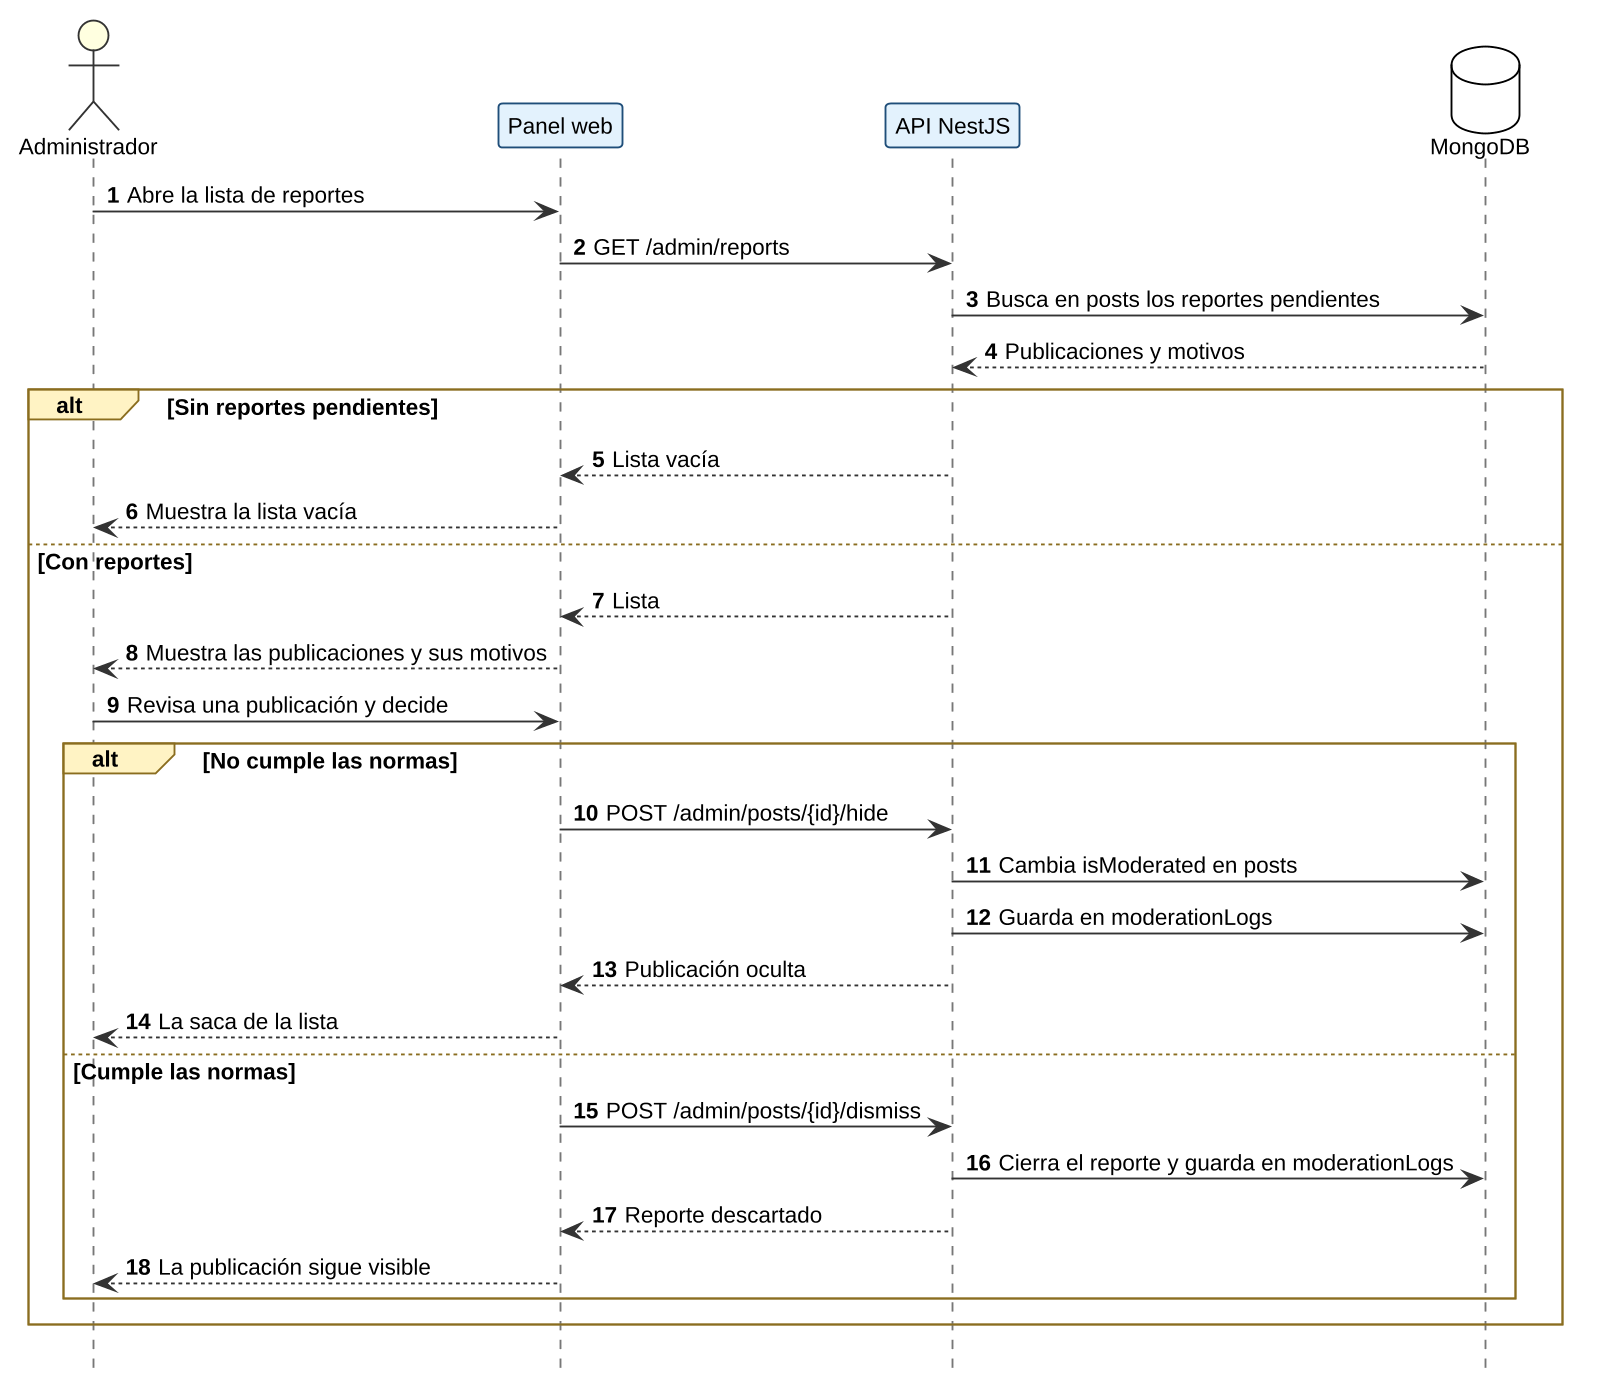
\includegraphics[width=0.95\textwidth,height=0.6\textheight,keepaspectratio]{figuras/secuencia/sec_cu11.png}
    \captionof{figure}{Diagrama de Secuencia -- CU-11: Revisar el contenido reportado.}
    \label{fig:sec_cu11}
\end{center}
El backend busca las publicaciones con reportes pendientes y las muestra con sus motivos. Si el administrador decide ocultar una publicación, esta sale del muro. Cualquiera sea la decisión, queda guardada en \texttt{moderationLogs} con quién la tomó y por qué.
\end{minipage}
\vspace{0.6cm}

\noindent\begin{minipage}{\linewidth}
\textbf{CU-12. Completar mi perfil y recibir un plan semanal}

Para el caso de uso CU-12 se genera el diagrama de secuencia que se muestra en la Figura \ref{fig:sec_cu12}.
\begin{center}
    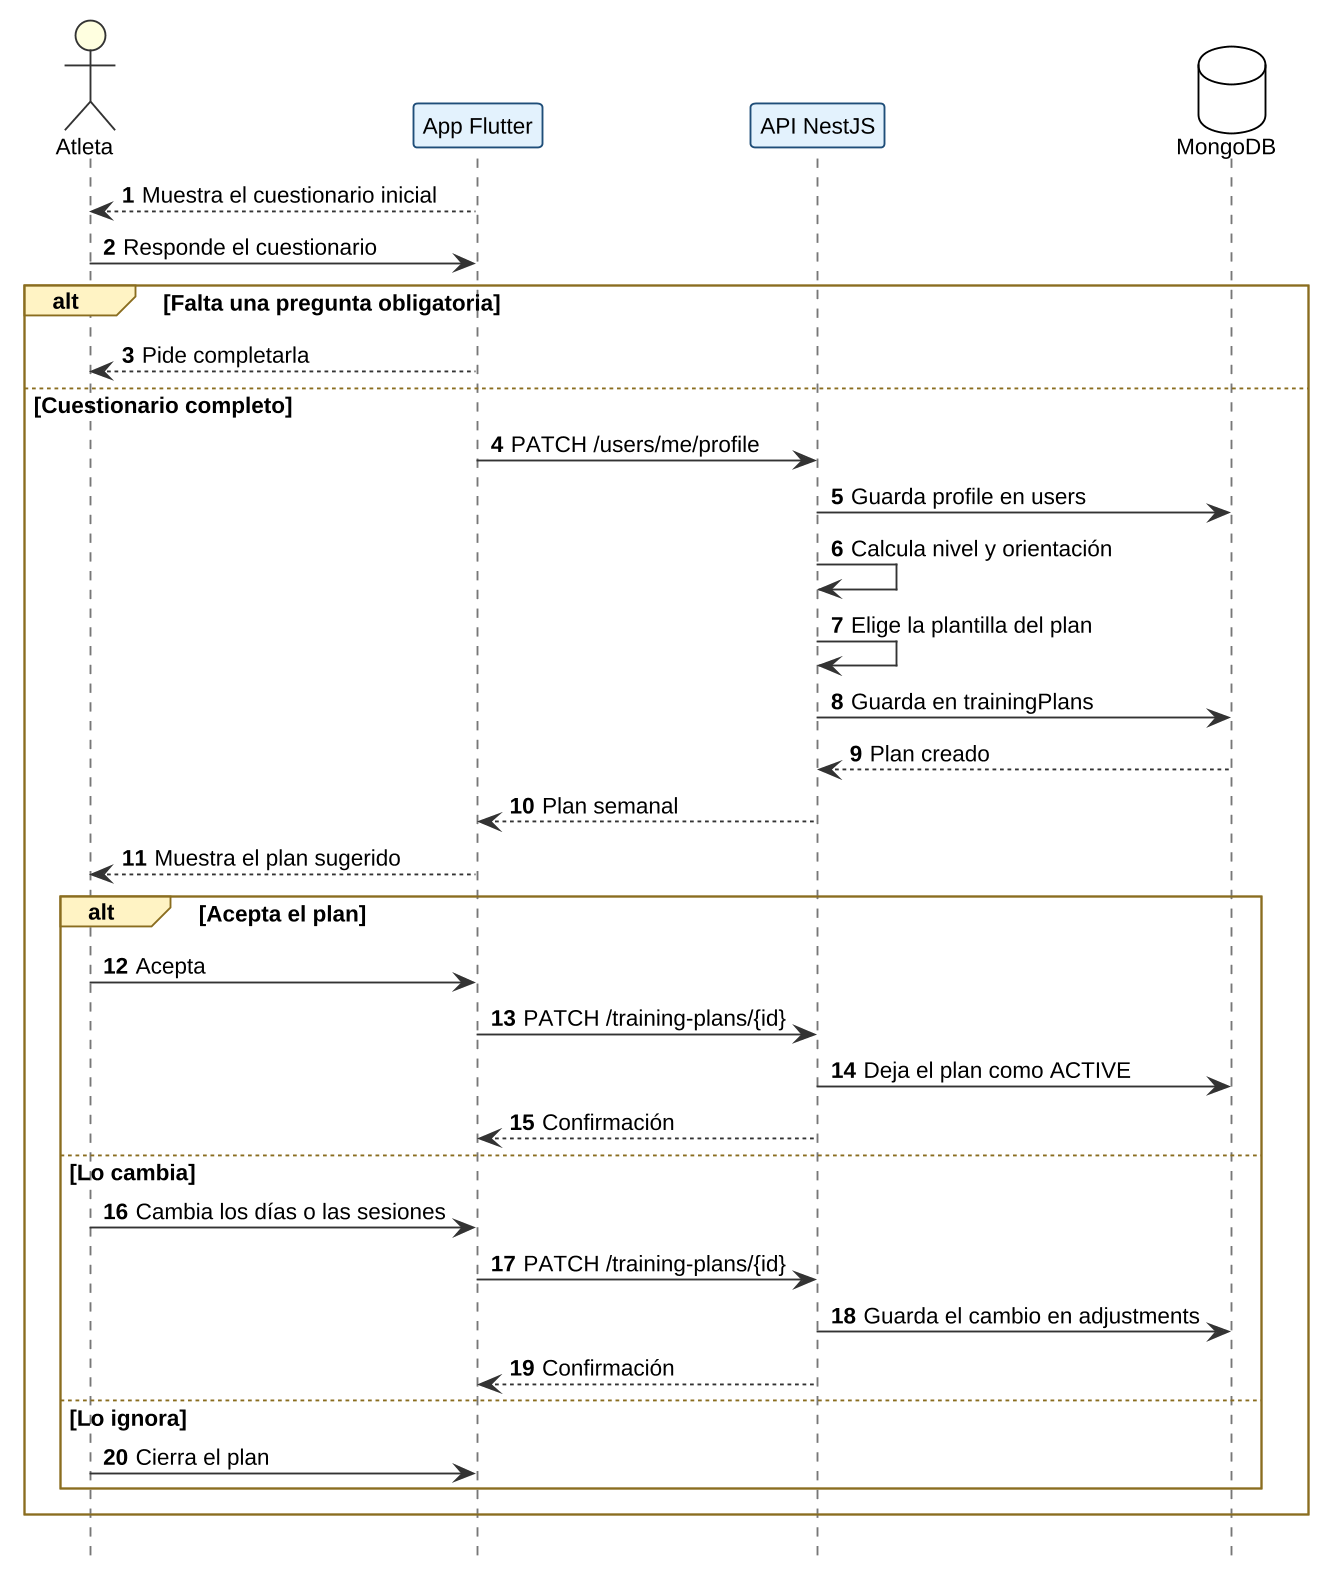
\includegraphics[width=0.95\textwidth,height=0.6\textheight,keepaspectratio]{figuras/secuencia/sec_cu12.png}
    \captionof{figure}{Diagrama de Secuencia -- CU-12: Completar mi perfil y recibir un plan semanal.}
    \label{fig:sec_cu12}
\end{center}
Con las respuestas del cuestionario, el backend actualiza el perfil, calcula el nivel y la orientación del usuario y elige la plantilla correspondiente, definida en el propio backend. El plan se guarda en \texttt{trainingPlans}. Si el usuario lo cambia, el cambio queda registrado en \texttt{adjustments}.
\end{minipage}
\vspace{0.6cm}

\noindent\begin{minipage}{\linewidth}
\textbf{CU-13. Agregar una publicación a mis módulos}

Para el caso de uso CU-13 se genera el diagrama de secuencia que se muestra en la Figura \ref{fig:sec_cu13}.
\begin{center}
    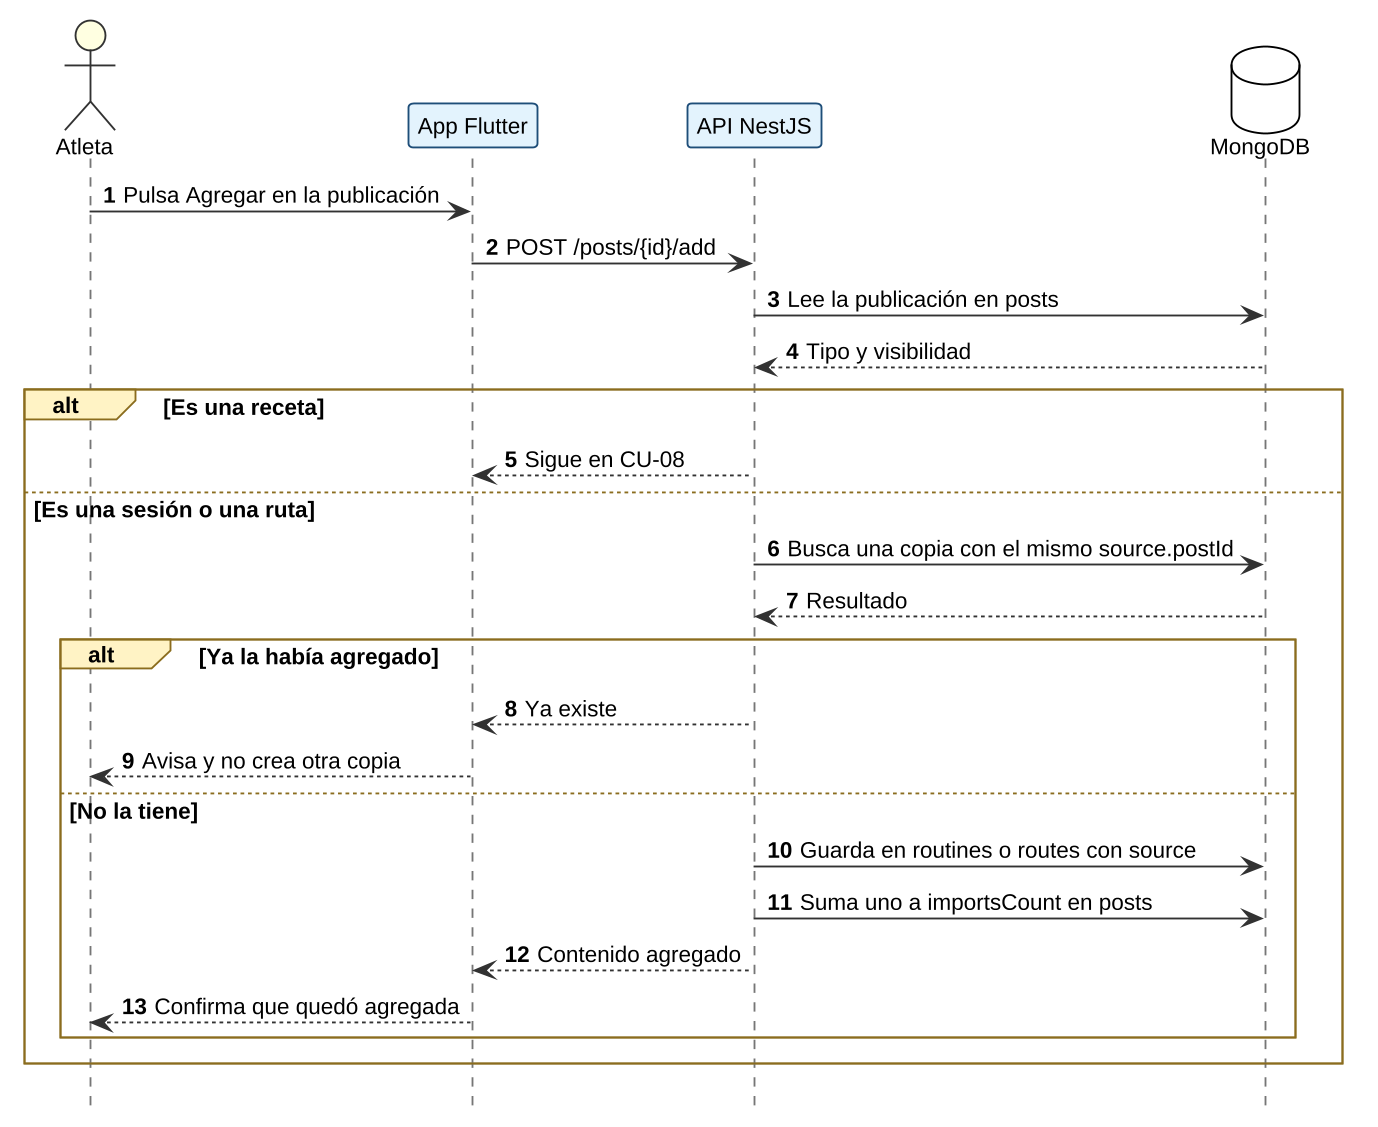
\includegraphics[width=0.95\textwidth,height=0.6\textheight,keepaspectratio]{figuras/secuencia/sec_cu13.png}
    \captionof{figure}{Diagrama de Secuencia -- CU-13: Agregar una publicación a mis módulos.}
    \label{fig:sec_cu13}
\end{center}
El backend identifica el tipo de publicación. Una sesión se copia en \texttt{routines} y una ruta en \texttt{routes}, con la referencia a su autor en el campo \texttt{source}, y se suma uno a \texttt{importsCount}. Antes revisa que el usuario no tenga ya esa copia. Las recetas siguen el flujo del CU-08.
\end{minipage}
\vspace{0.6cm}

\noindent\begin{minipage}{\linewidth}
\textbf{CU-14. Seguir a otro usuario}

Para el caso de uso CU-14 se genera el diagrama de secuencia que se muestra en la Figura \ref{fig:sec_cu14}.
\begin{center}
    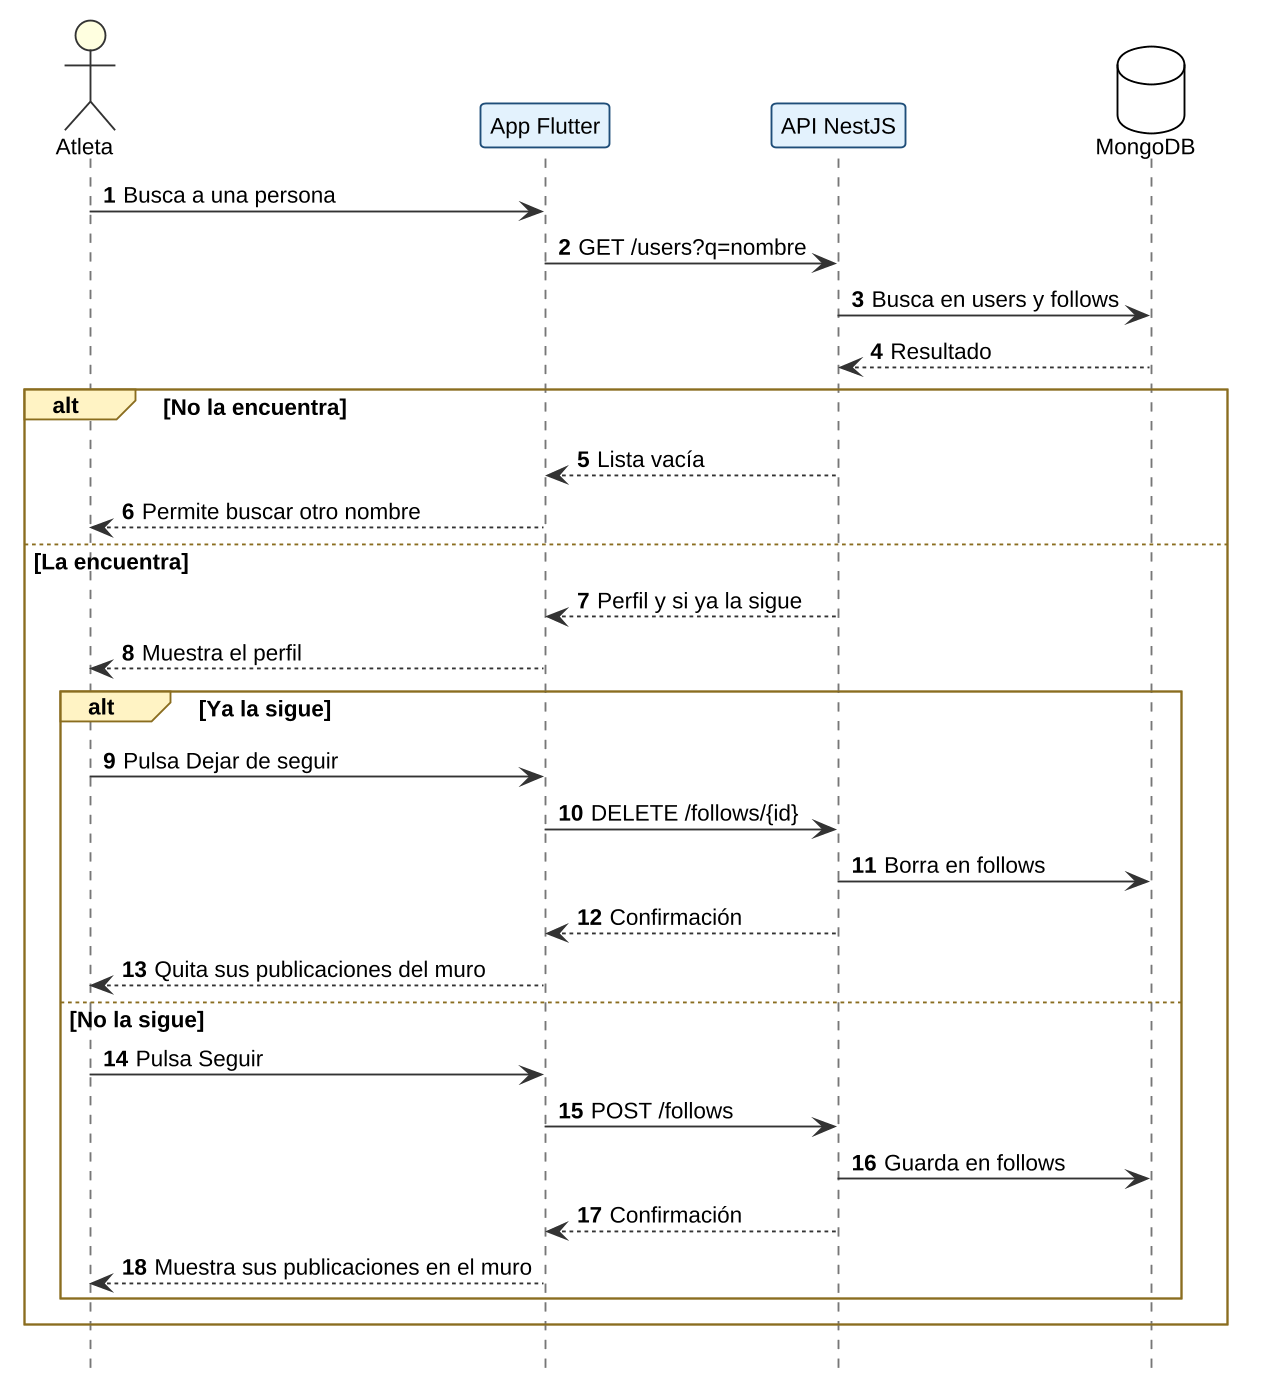
\includegraphics[width=0.95\textwidth,height=0.6\textheight,keepaspectratio]{figuras/secuencia/sec_cu14.png}
    \captionof{figure}{Diagrama de Secuencia -- CU-14: Seguir a otro usuario.}
    \label{fig:sec_cu14}
\end{center}
El backend busca a la persona y responde si el usuario ya la sigue. Seguir a alguien crea un documento en \texttt{follows}, y dejar de seguirlo lo borra. El muro se arma con estas relaciones (CU-23).
\end{minipage}
\vspace{0.6cm}

\noindent\begin{minipage}{\linewidth}
\textbf{CU-15. Registrar un producto con su código de barras}

Para el caso de uso CU-15 se genera el diagrama de secuencia que se muestra en la Figura \ref{fig:sec_cu15}.
\begin{center}
    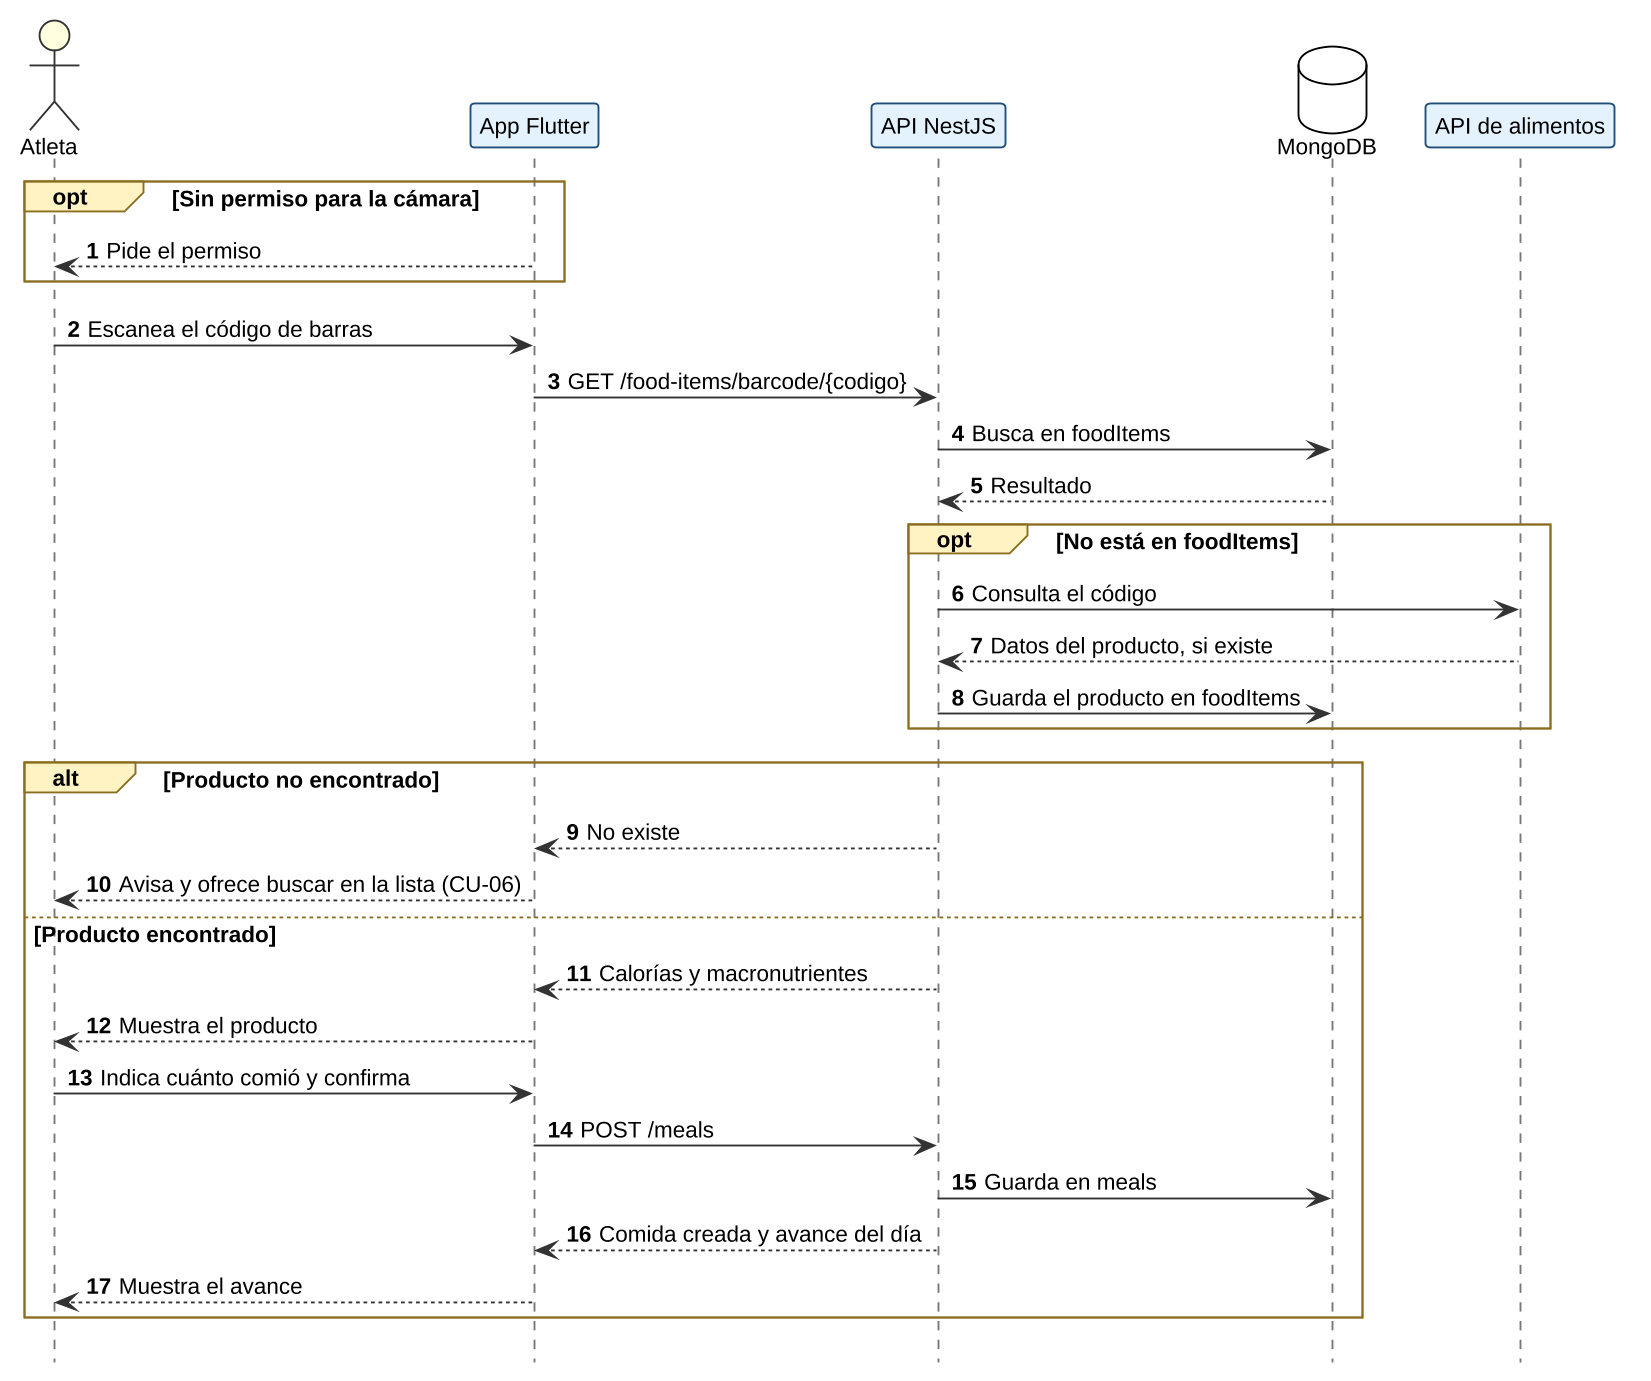
\includegraphics[width=0.95\textwidth,height=0.6\textheight,keepaspectratio]{figuras/secuencia/sec_cu15.png}
    \captionof{figure}{Diagrama de Secuencia -- CU-15: Registrar un producto con su código de barras.}
    \label{fig:sec_cu15}
\end{center}
El backend busca primero el código en \texttt{foodItems}. Si no está, consulta la API de alimentos y guarda el producto, para que las siguientes consultas sean más rápidas. Si el producto no existe en ninguna de las dos fuentes, se ofrece buscarlo en la lista.
\end{minipage}
\vspace{0.6cm}

\noindent\begin{minipage}{\linewidth}
\textbf{CU-16. Contar mi comida con mis palabras}

Para el caso de uso CU-16 se genera el diagrama de secuencia que se muestra en la Figura \ref{fig:sec_cu16}.
\begin{center}
    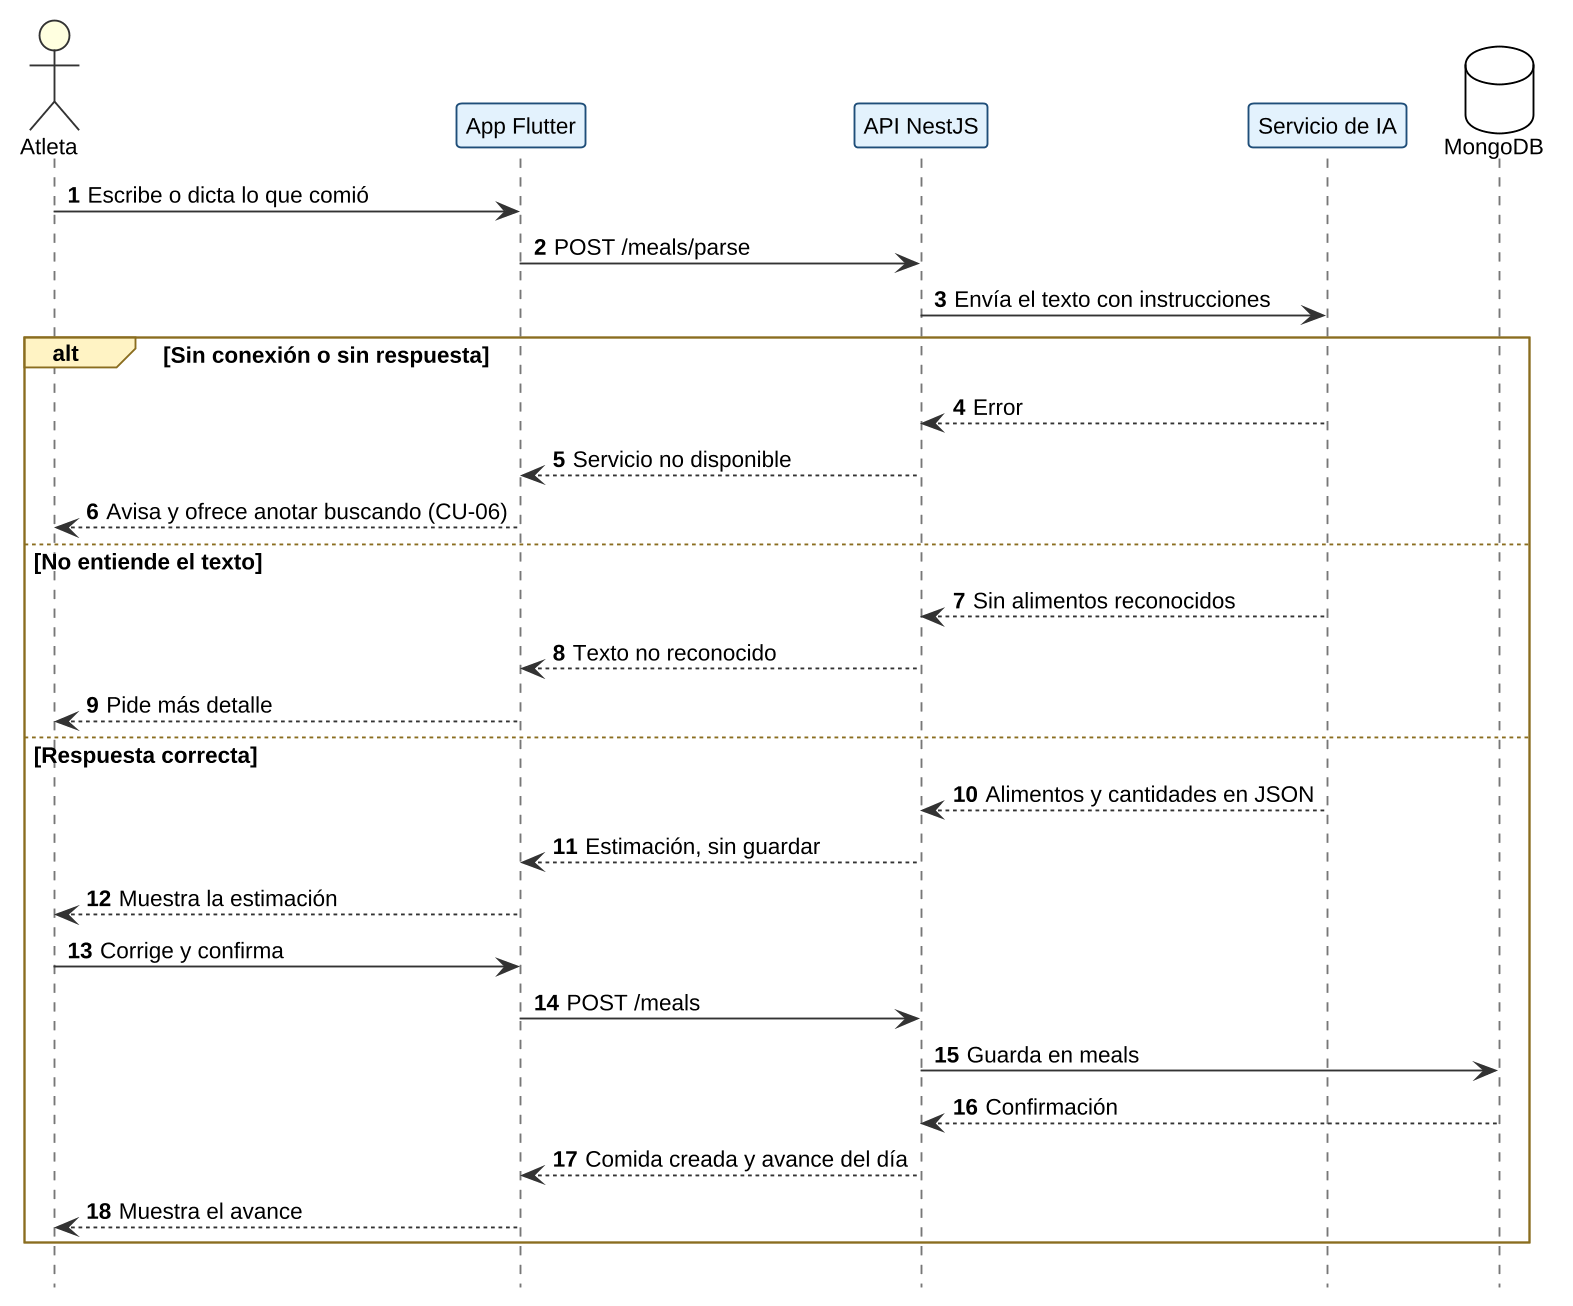
\includegraphics[width=0.95\textwidth,height=0.6\textheight,keepaspectratio]{figuras/secuencia/sec_cu16.png}
    \captionof{figure}{Diagrama de Secuencia -- CU-16: Contar mi comida con mis palabras.}
    \label{fig:sec_cu16}
\end{center}
El flujo es parecido al del CU-07, pero con texto en vez de una foto. El backend envía la descripción al servicio de IA y devuelve una estimación sin guardarla. Si el texto no se entiende, se pide más detalle. La comida se guarda solo cuando el usuario confirma.
\end{minipage}
\vspace{0.6cm}

\noindent\begin{minipage}{\linewidth}
\textbf{CU-17. Registrar una sesión de cardio sin reloj}

Para el caso de uso CU-17 se genera el diagrama de secuencia que se muestra en la Figura \ref{fig:sec_cu17}.
\begin{center}
    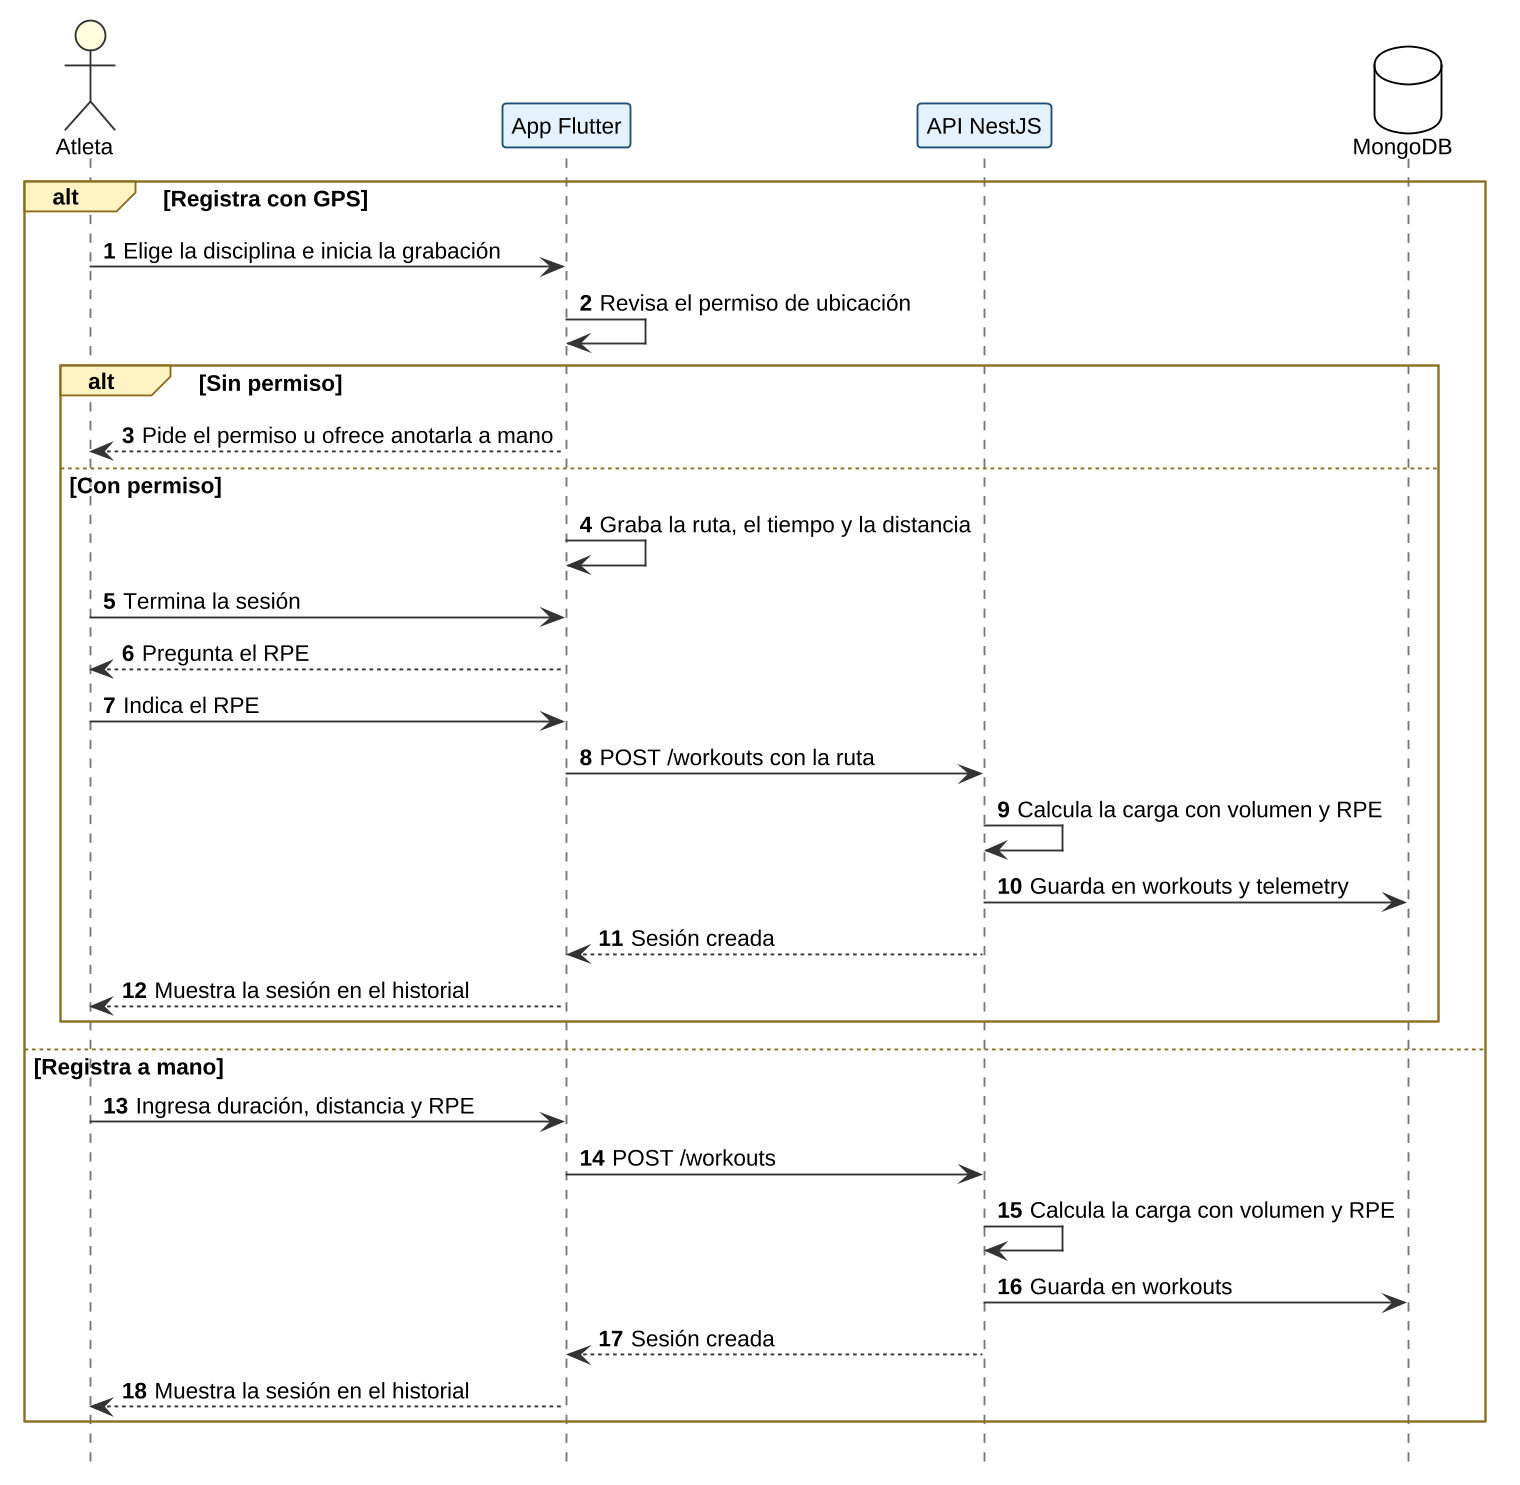
\includegraphics[width=0.95\textwidth,height=0.6\textheight,keepaspectratio]{figuras/secuencia/sec_cu17.png}
    \captionof{figure}{Diagrama de Secuencia -- CU-17: Registrar una sesión de cardio sin reloj.}
    \label{fig:sec_cu17}
\end{center}
La grabación con GPS ocurre en el teléfono, por lo que no necesita conexión mientras dura la sesión. Al terminar, la aplicación envía la ruta y el RPE. Sin dispositivos externos, la carga se calcula con el volumen de la sesión y el RPE. El registro a mano sigue el mismo camino, pero sin ruta.
\end{minipage}
\vspace{0.6cm}

\noindent\begin{minipage}{\linewidth}
\textbf{CU-18. Ver mis metas de alimentación del día}

Para el caso de uso CU-18 se genera el diagrama de secuencia que se muestra en la Figura \ref{fig:sec_cu18}.
\begin{center}
    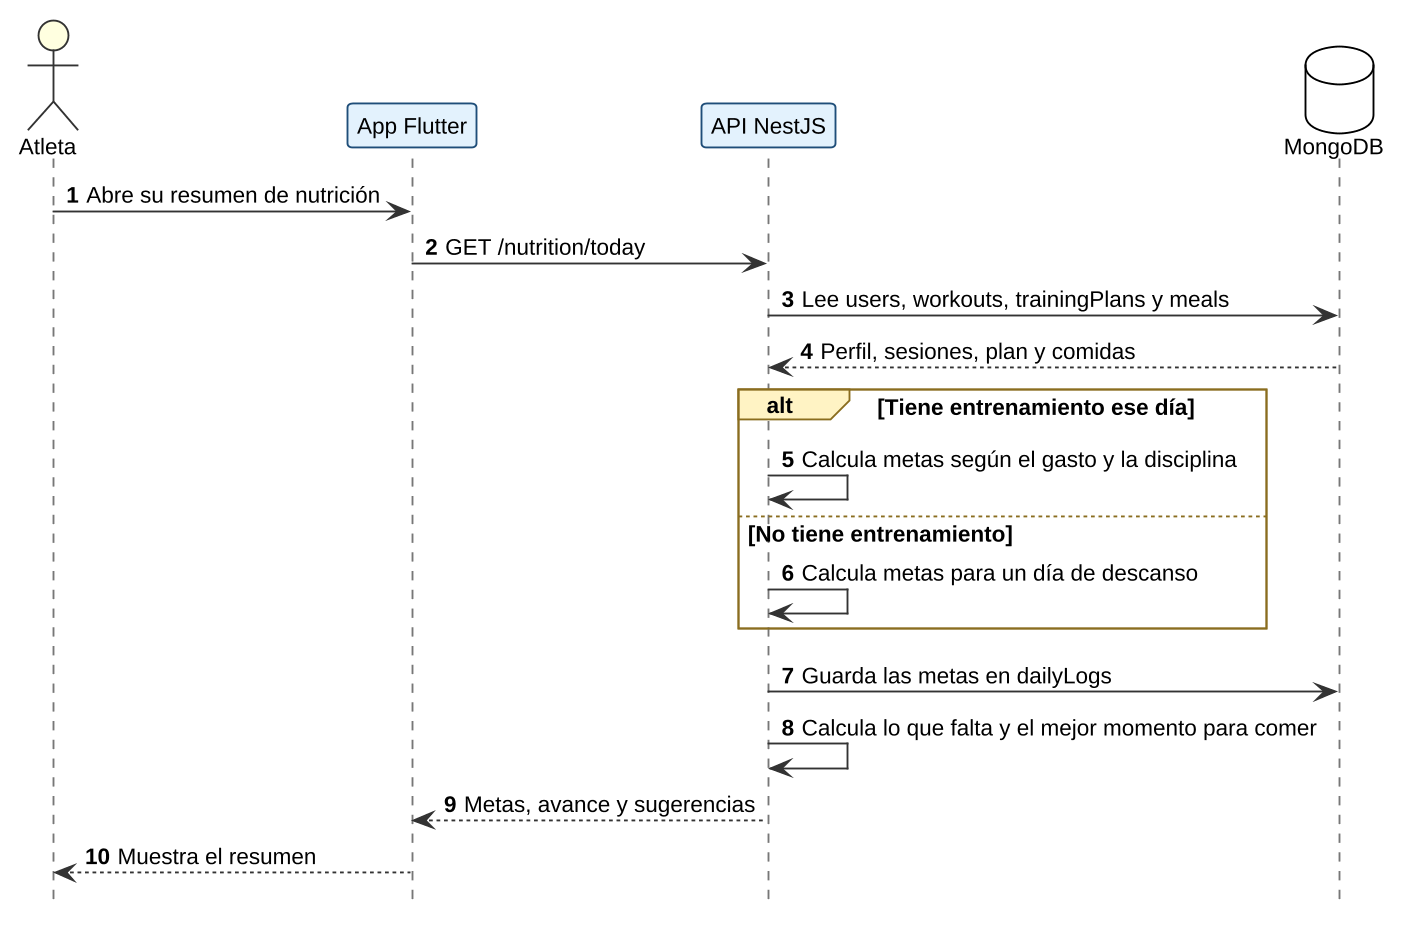
\includegraphics[width=0.95\textwidth,height=0.6\textheight,keepaspectratio]{figuras/secuencia/sec_cu18.png}
    \captionof{figure}{Diagrama de Secuencia -- CU-18: Ver mis metas de alimentación del día.}
    \label{fig:sec_cu18}
\end{center}
El backend lee el perfil, las sesiones, el plan y las comidas del día. Con eso calcula las metas según el gasto estimado y la disciplina, o las metas de un día de descanso si no hay entrenamiento. Las guarda en \texttt{dailyLogs} y responde con el avance y las sugerencias de horario.
\end{minipage}
\vspace{0.6cm}

\noindent\begin{minipage}{\linewidth}
\textbf{CU-19. Revisar mi progreso}

Para el caso de uso CU-19 se genera el diagrama de secuencia que se muestra en la Figura \ref{fig:sec_cu19}.
\begin{center}
    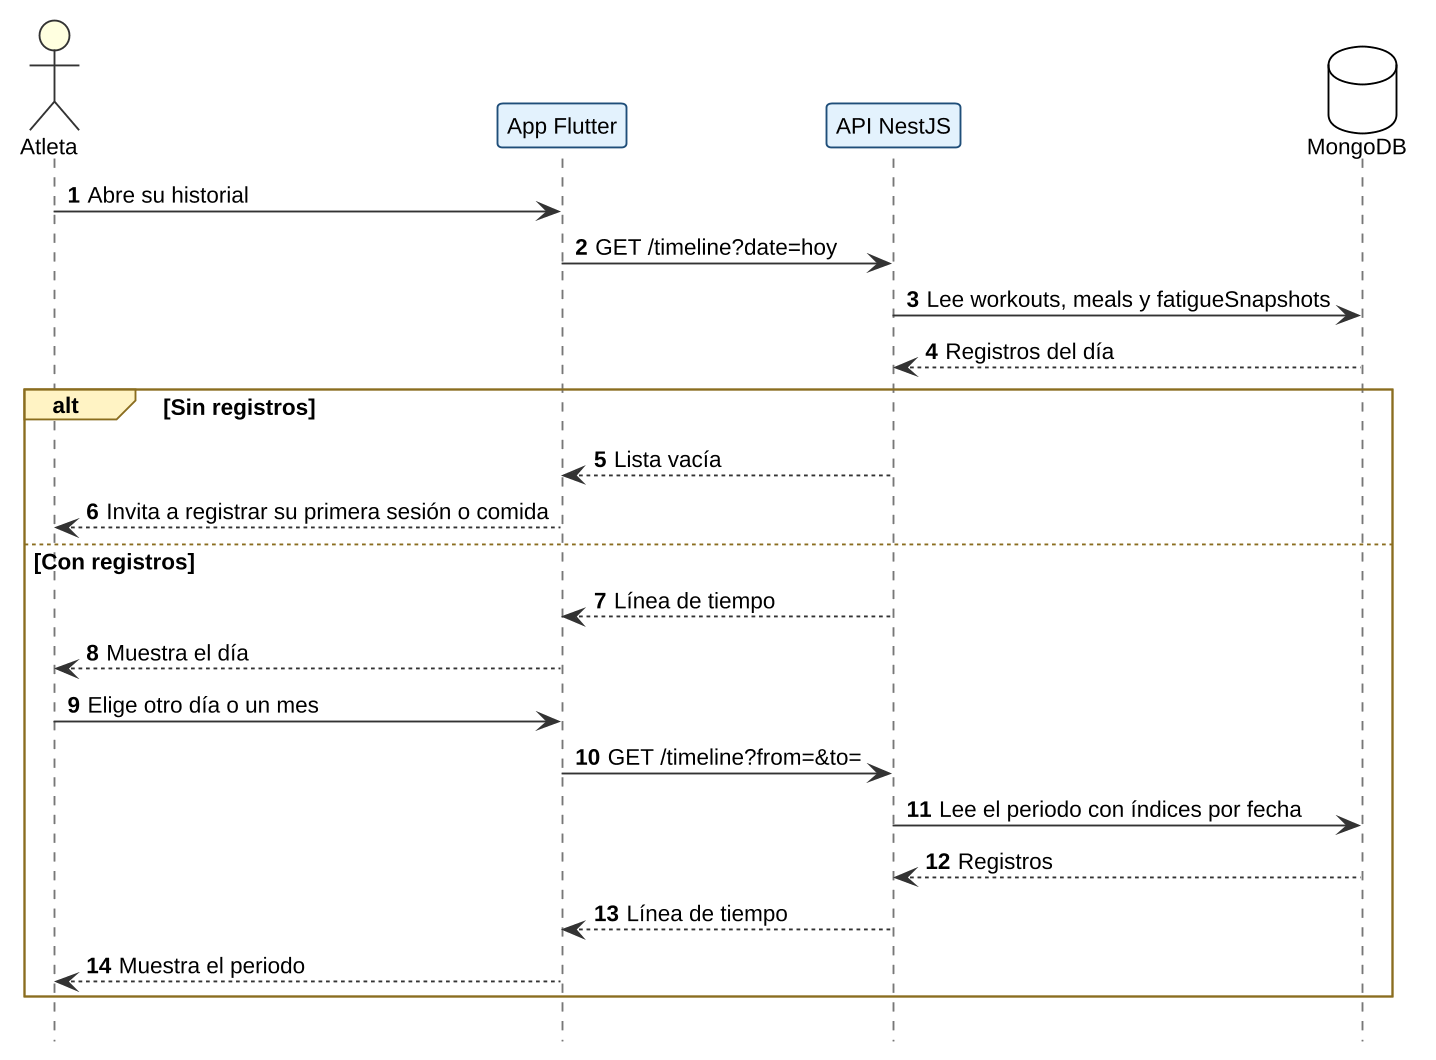
\includegraphics[width=0.95\textwidth,height=0.6\textheight,keepaspectratio]{figuras/secuencia/sec_cu19.png}
    \captionof{figure}{Diagrama de Secuencia -- CU-19: Revisar mi progreso.}
    \label{fig:sec_cu19}
\end{center}
El historial se arma consultando por usuario y fecha en \texttt{workouts}, \texttt{meals} y \texttt{fatigueSnapshots}. Los índices compuestos por usuario y fecha hacen que esta consulta sea rápida, tanto para un día como para un mes.
\end{minipage}
\vspace{0.6cm}

\noindent\begin{minipage}{\linewidth}
\textbf{CU-20. Anotar cómo me sentí}

Para el caso de uso CU-20 se genera el diagrama de secuencia que se muestra en la Figura \ref{fig:sec_cu20}.
\begin{center}
    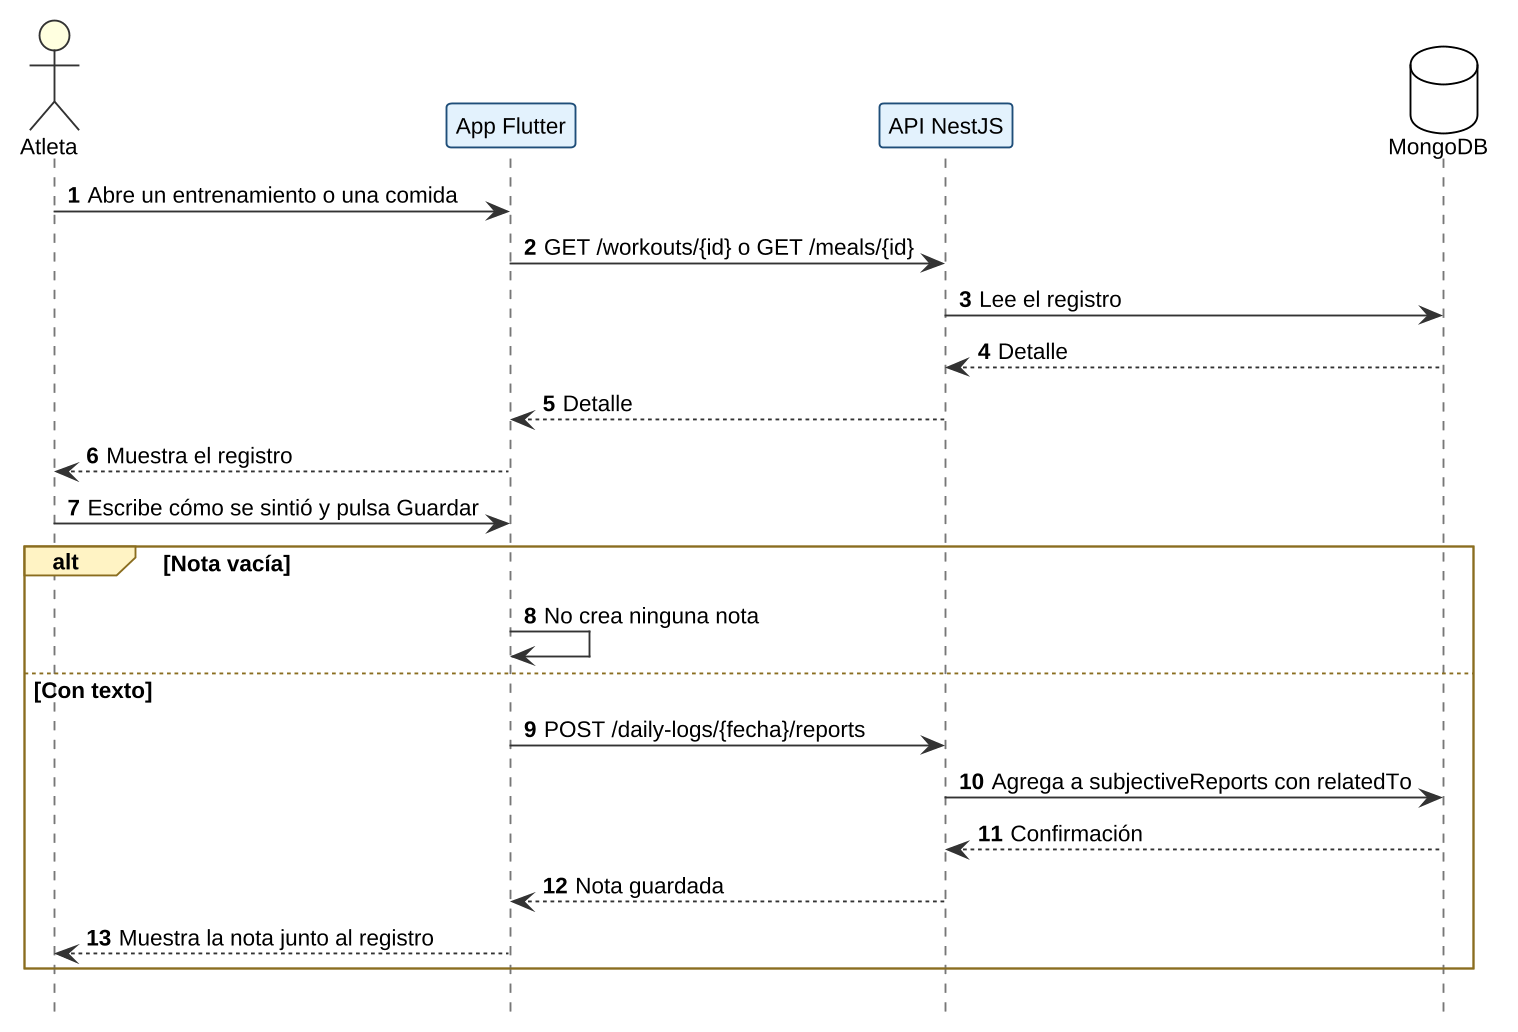
\includegraphics[width=0.95\textwidth,height=0.6\textheight,keepaspectratio]{figuras/secuencia/sec_cu20.png}
    \captionof{figure}{Diagrama de Secuencia -- CU-20: Anotar cómo me sentí.}
    \label{fig:sec_cu20}
\end{center}
La nota se guarda en \texttt{subjectiveReports}, dentro del registro diario, con el campo \texttt{relatedTo}, que indica a qué entrenamiento o comida pertenece. Si el usuario no escribe nada, la aplicación no hace ninguna llamada al backend.
\end{minipage}
\vspace{0.6cm}

\noindent\begin{minipage}{\linewidth}
\textbf{CU-21. Controlar mis datos personales}

Para el caso de uso CU-21 se genera el diagrama de secuencia que se muestra en la Figura \ref{fig:sec_cu21}.
\begin{center}
    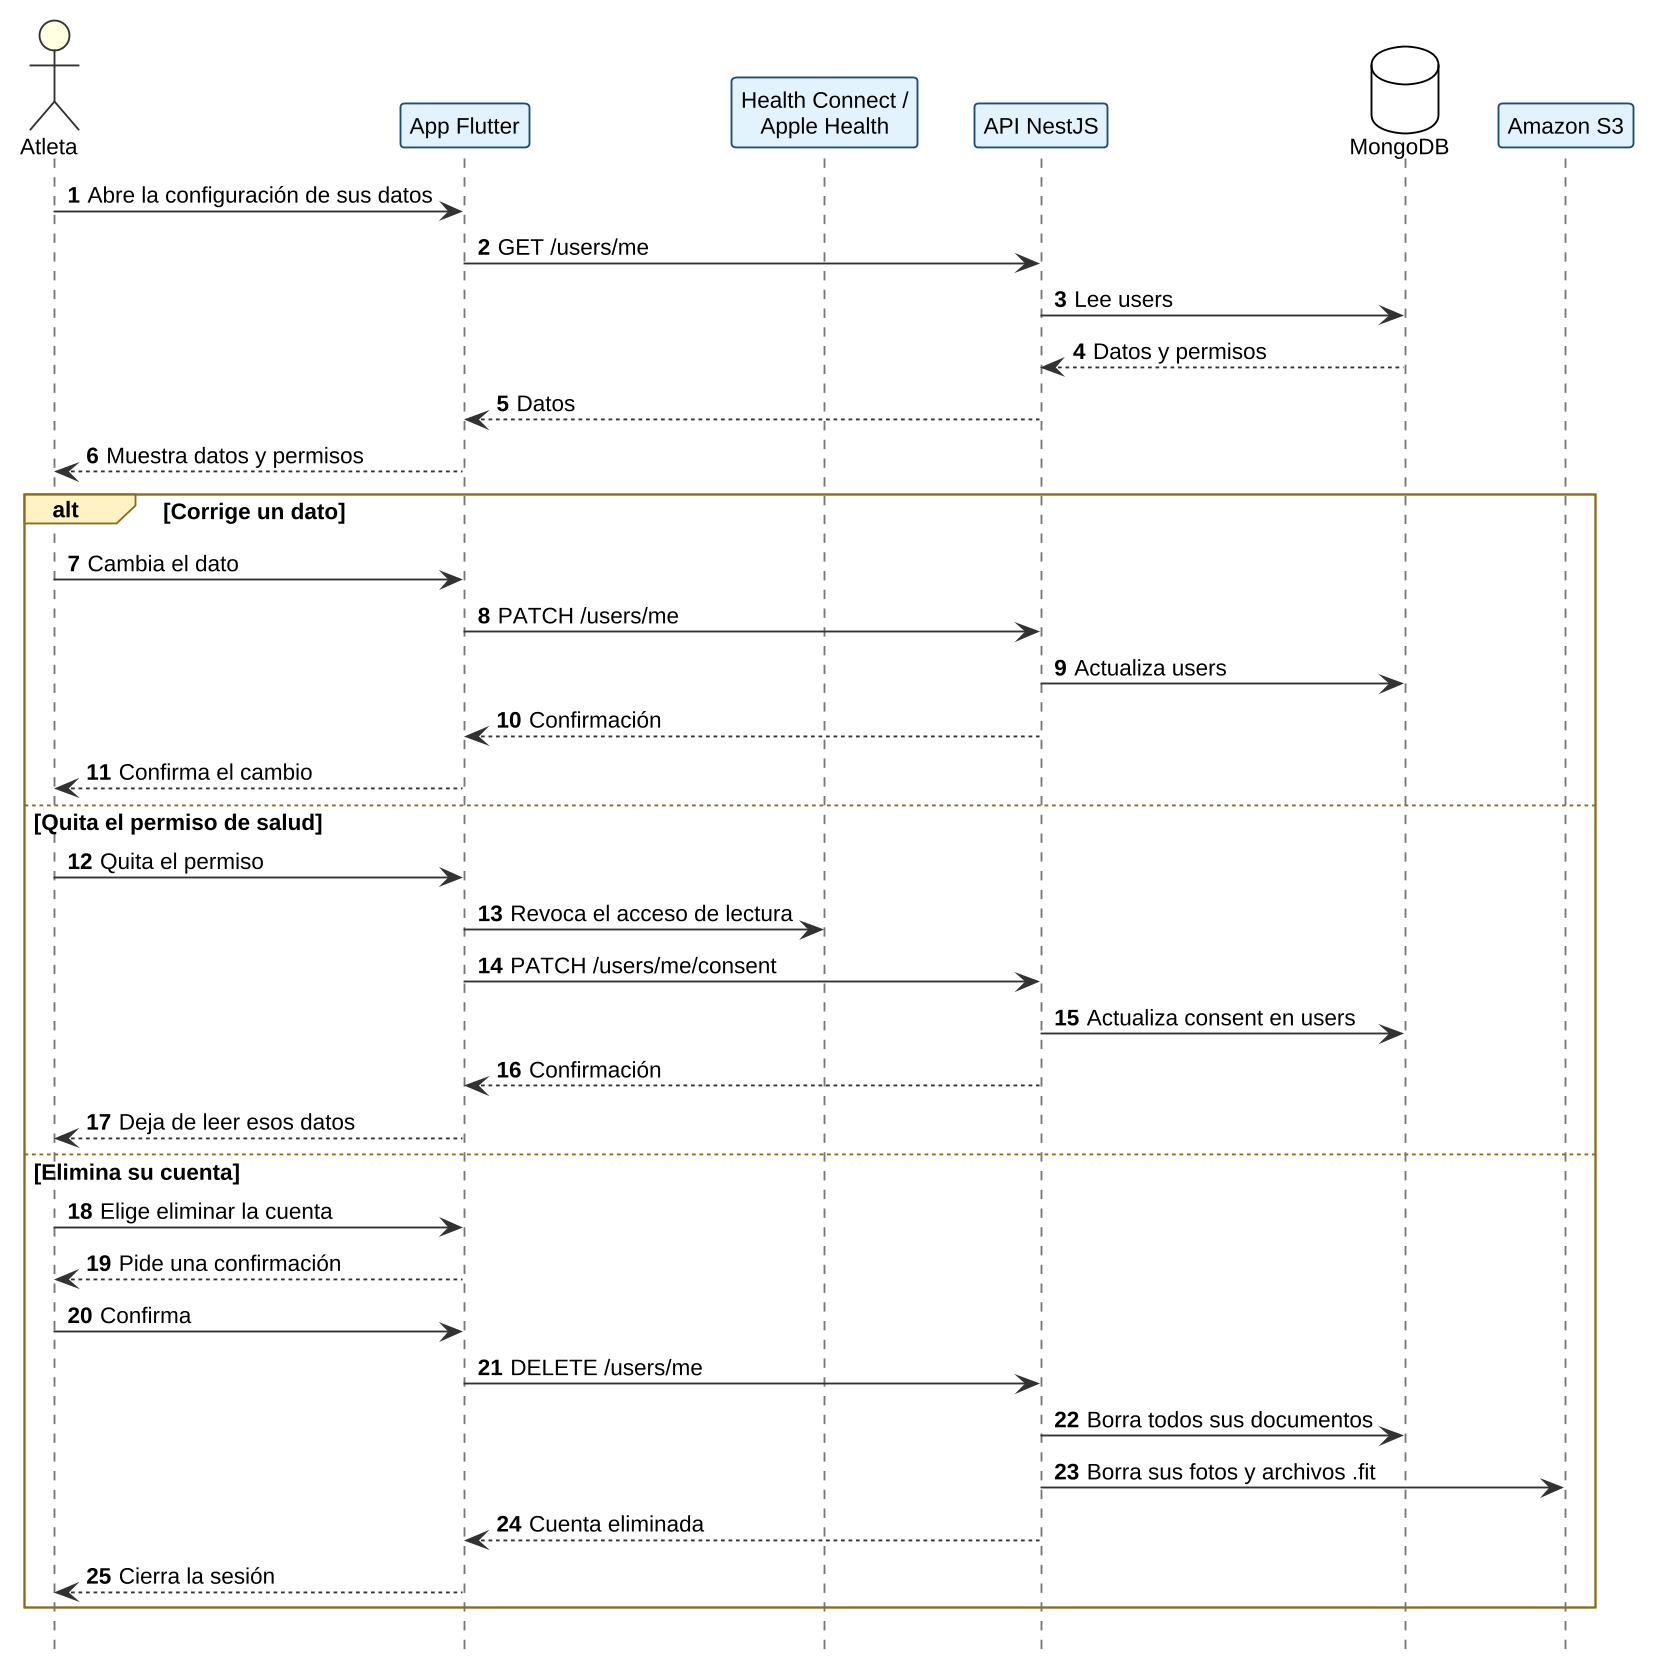
\includegraphics[width=0.95\textwidth,height=0.6\textheight,keepaspectratio]{figuras/secuencia/sec_cu21.png}
    \captionof{figure}{Diagrama de Secuencia -- CU-21: Controlar mis datos personales.}
    \label{fig:sec_cu21}
\end{center}
Los cambios de datos se guardan en \texttt{users}. Quitar el permiso de salud corta el acceso en el teléfono y queda registrado en \texttt{consent}. Al eliminar la cuenta, el backend borra todos los documentos del usuario en MongoDB y sus archivos en Amazon S3, como exige la Ley N° 19.628.
\end{minipage}
\vspace{0.6cm}

\noindent\begin{minipage}{\linewidth}
\textbf{CU-22. Reportar una publicación}

Para el caso de uso CU-22 se genera el diagrama de secuencia que se muestra en la Figura \ref{fig:sec_cu22}.
\begin{center}
    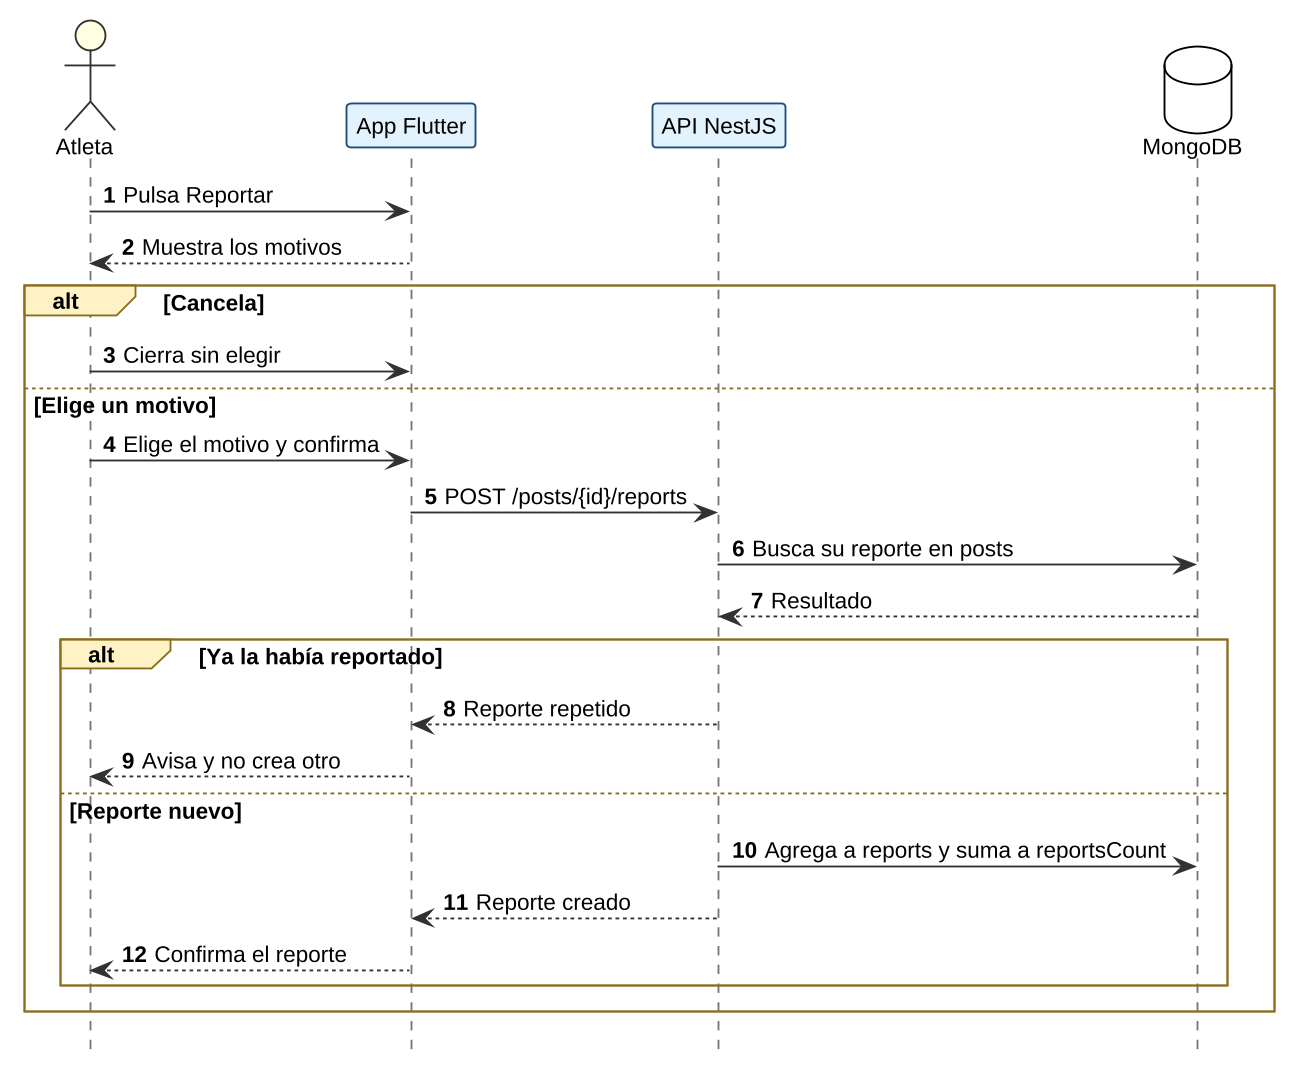
\includegraphics[width=0.95\textwidth,height=0.6\textheight,keepaspectratio]{figuras/secuencia/sec_cu22.png}
    \captionof{figure}{Diagrama de Secuencia -- CU-22: Reportar una publicación.}
    \label{fig:sec_cu22}
\end{center}
El backend revisa en el arreglo \texttt{reports} de la publicación que el usuario no la haya reportado antes. Si no lo ha hecho, agrega el reporte con su motivo y suma uno a \texttt{reportsCount}. Con esto la publicación aparece en la lista de revisión del administrador (CU-11).
\end{minipage}
\vspace{0.6cm}

\noindent\begin{minipage}{\linewidth}
\textbf{CU-23. Ver el muro de la comunidad}

Para el caso de uso CU-23 se genera el diagrama de secuencia que se muestra en la Figura \ref{fig:sec_cu23}.
\begin{center}
    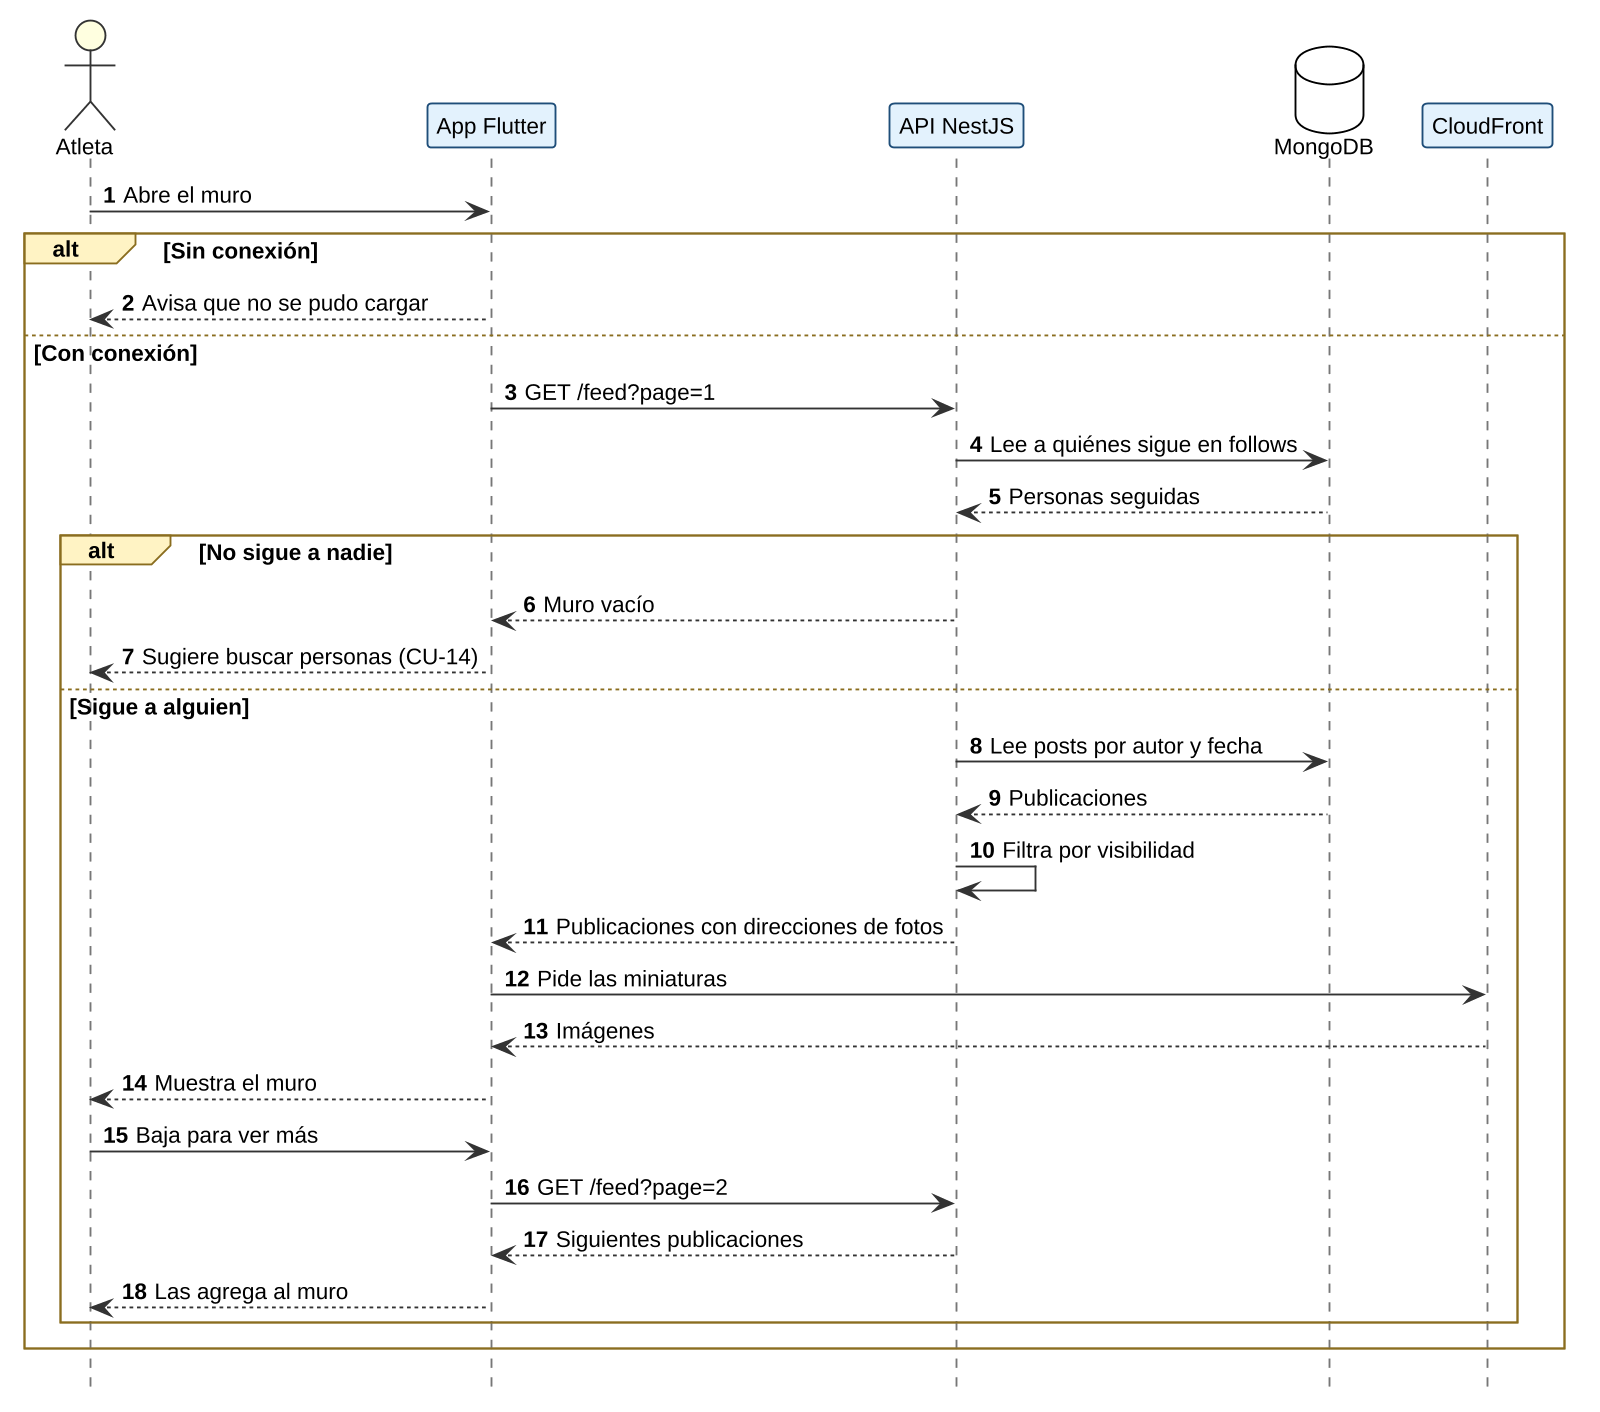
\includegraphics[width=0.95\textwidth,height=0.6\textheight,keepaspectratio]{figuras/secuencia/sec_cu23.png}
    \captionof{figure}{Diagrama de Secuencia -- CU-23: Ver el muro de la comunidad.}
    \label{fig:sec_cu23}
\end{center}
El backend lee a quiénes sigue el usuario en \texttt{follows}, busca sus publicaciones más recientes en \texttt{posts} y filtra las que puede ver según su visibilidad. La respuesta llega por páginas y solo trae las direcciones de las fotos. La aplicación las pide después a CloudFront, sin pasar por el backend.
\end{minipage}
\vspace{0.6cm}

\noindent\begin{minipage}{\linewidth}
\textbf{CU-24. Contratar el plan premium}

Para el caso de uso CU-24 se genera el diagrama de secuencia que se muestra en la Figura \ref{fig:sec_cu24}.
\begin{center}
    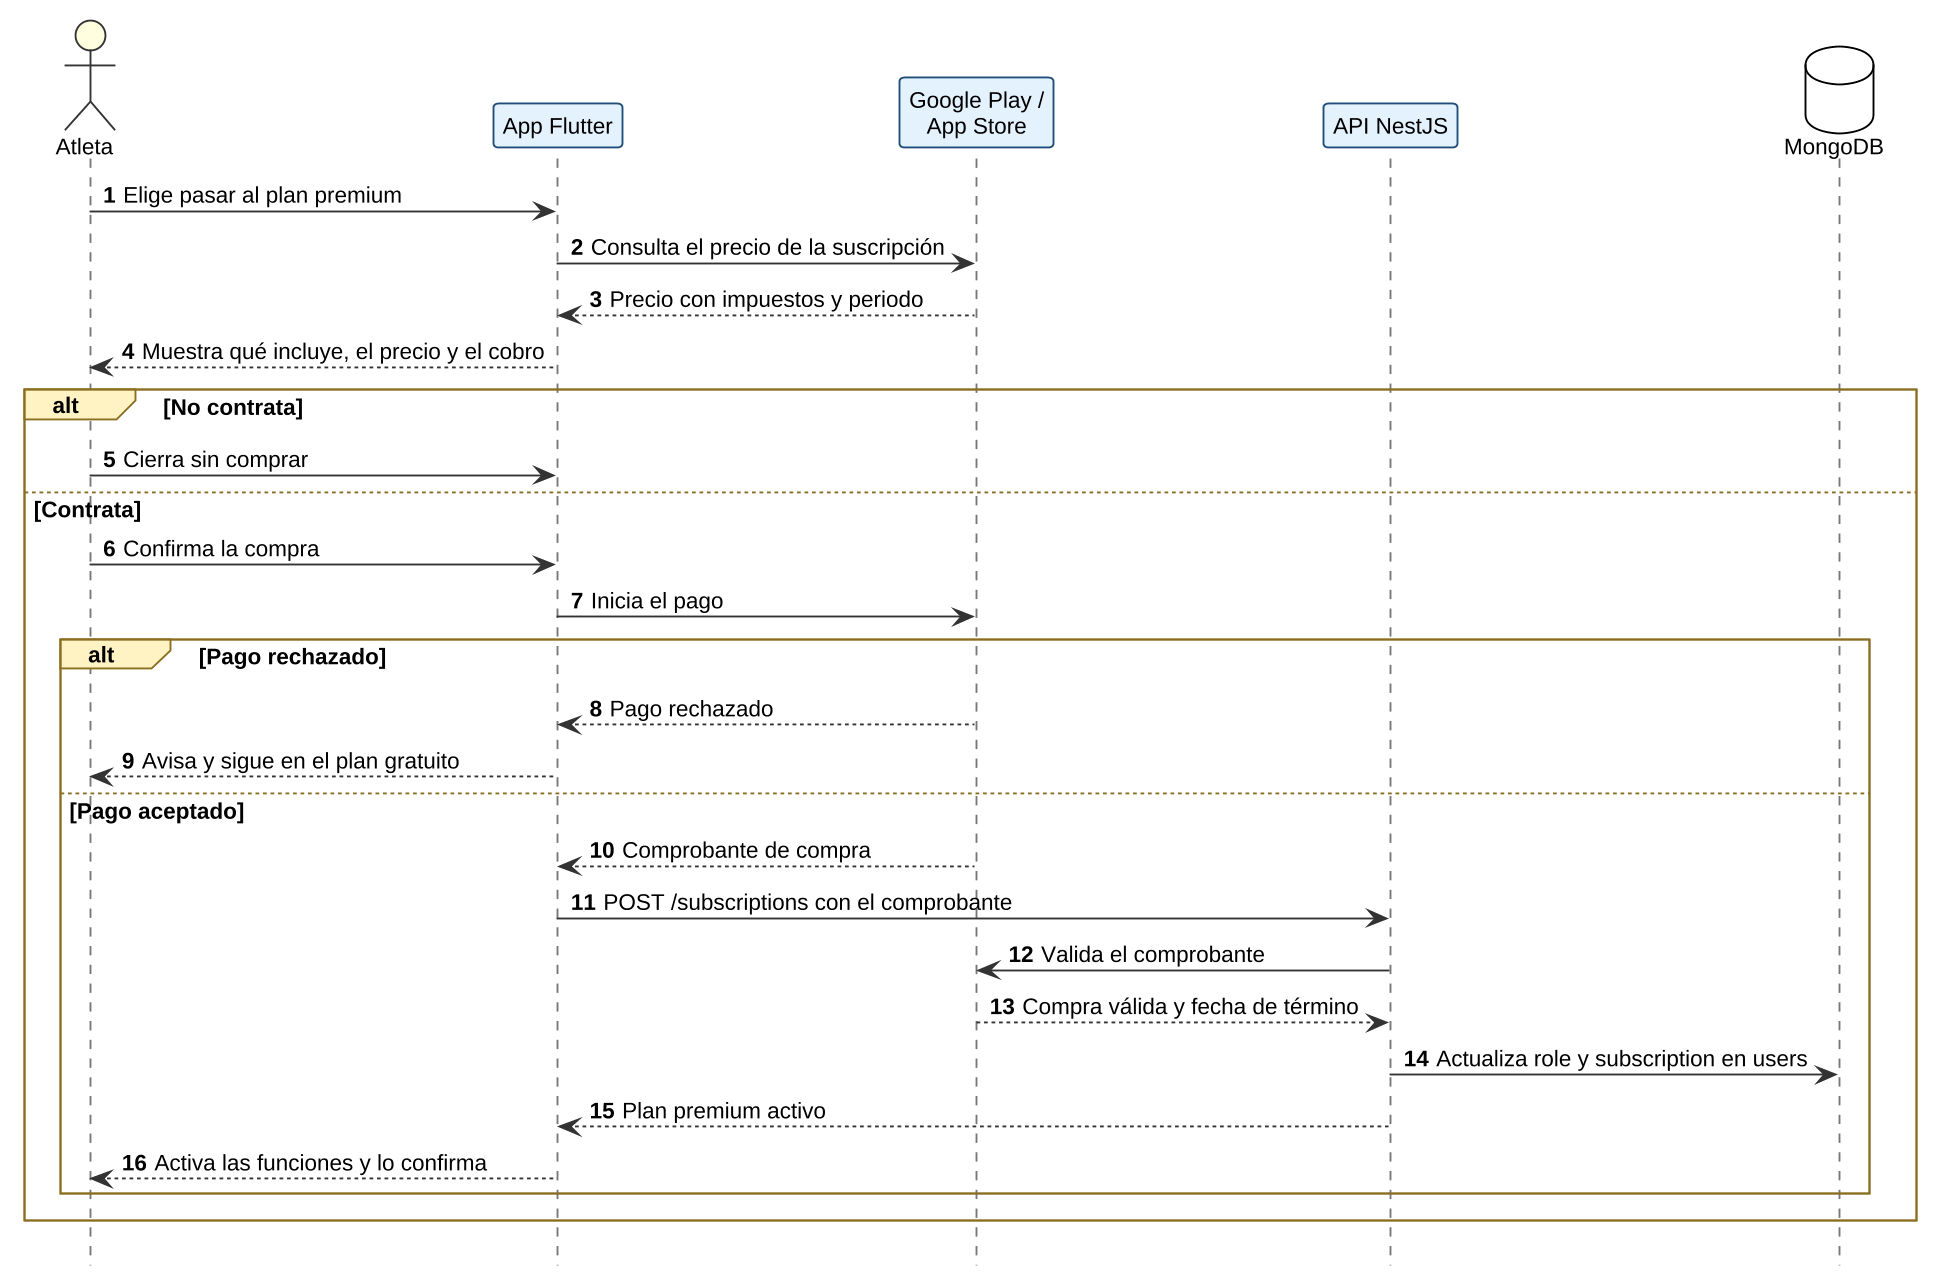
\includegraphics[width=0.95\textwidth,height=0.6\textheight,keepaspectratio]{figuras/secuencia/sec_cu24.png}
    \captionof{figure}{Diagrama de Secuencia -- CU-24: Contratar el plan premium.}
    \label{fig:sec_cu24}
\end{center}
El precio viene de la tienda, para mostrar el valor final con impuestos. El pago ocurre completo en Google Play o App Store, por lo que el sistema no maneja datos de tarjetas. Al terminar, la aplicación envía el comprobante al backend, que lo valida con la tienda antes de activar el plan en \texttt{users}.
\end{minipage}
\vspace{0.6cm}

\noindent\begin{minipage}{\linewidth}
\textbf{CU-25. Cancelar mi suscripción}

Para el caso de uso CU-25 se genera el diagrama de secuencia que se muestra en la Figura \ref{fig:sec_cu25}.
\begin{center}
    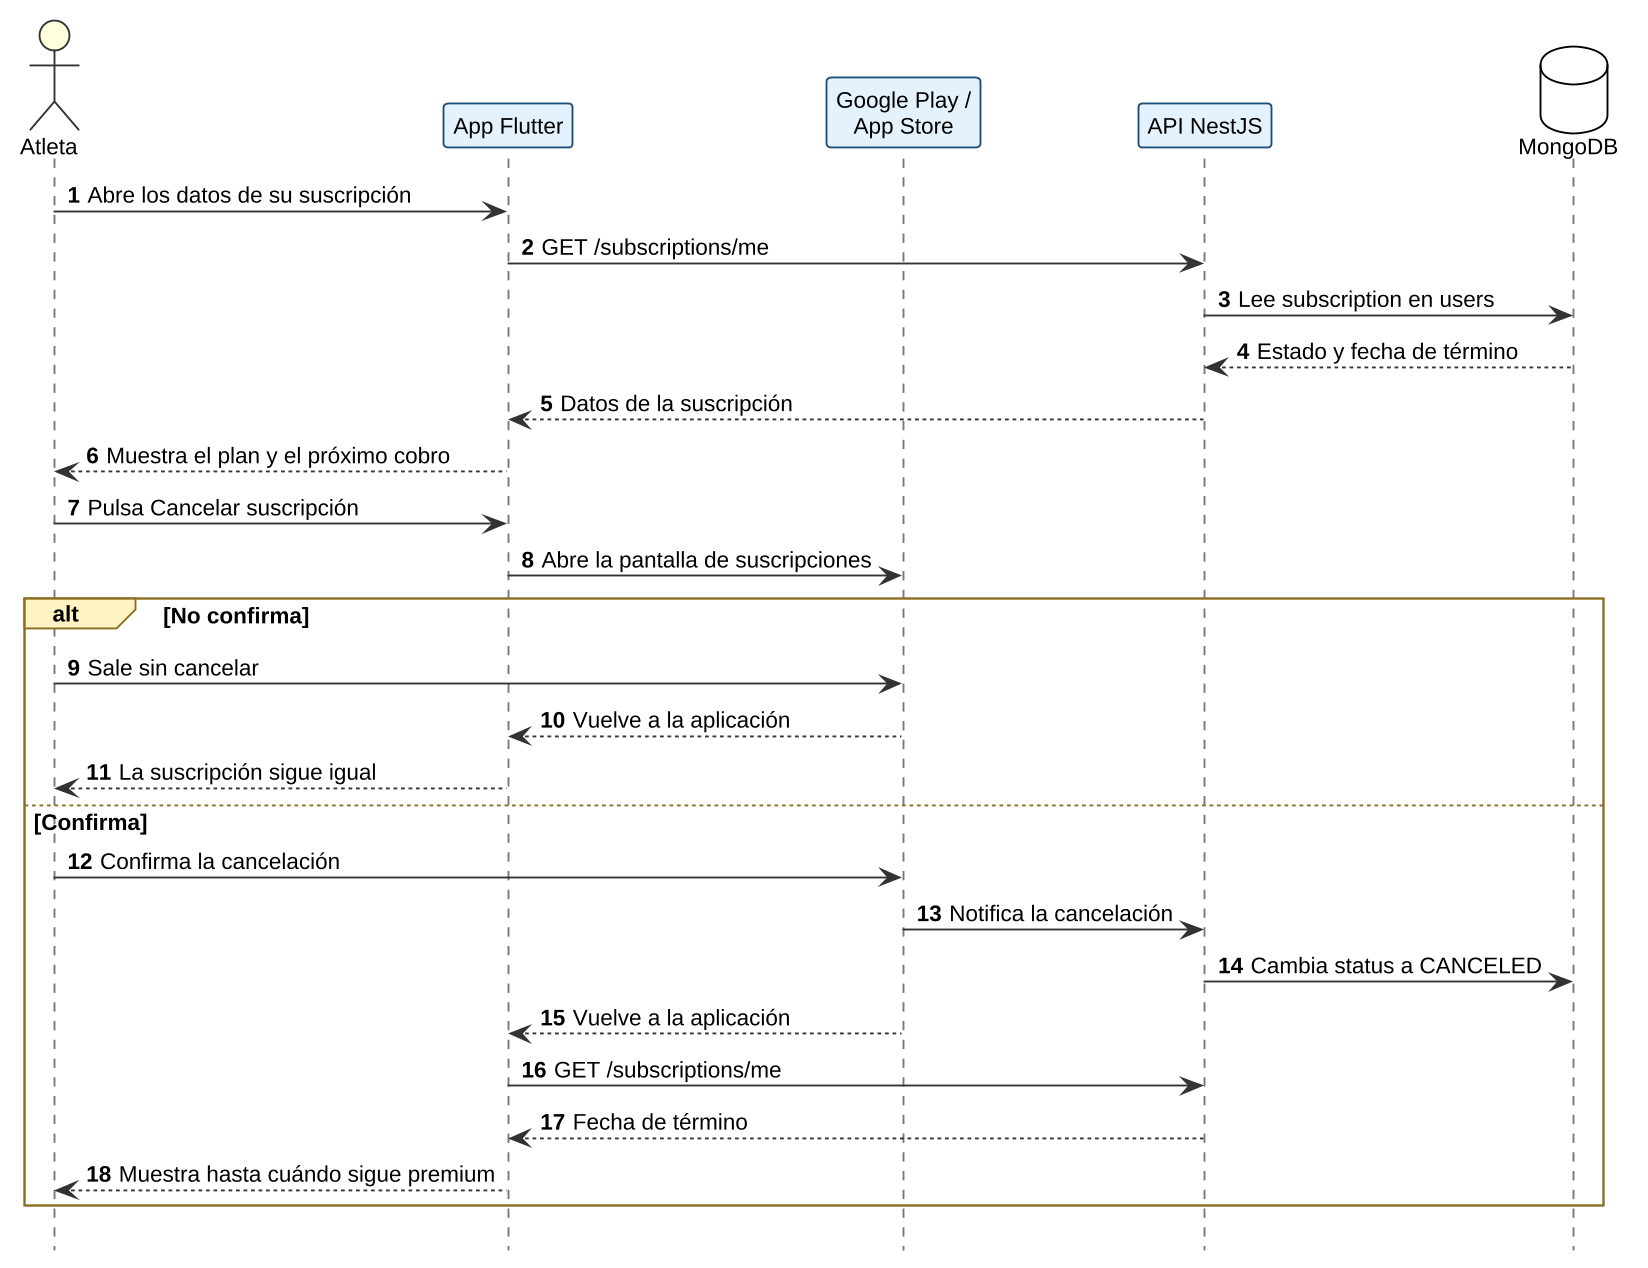
\includegraphics[width=0.95\textwidth,height=0.6\textheight,keepaspectratio]{figuras/secuencia/sec_cu25.png}
    \captionof{figure}{Diagrama de Secuencia -- CU-25: Cancelar mi suscripción.}
    \label{fig:sec_cu25}
\end{center}
La cancelación se confirma en la pantalla de suscripciones de la tienda. La tienda avisa al backend, que cambia el estado de la suscripción a \texttt{CANCELED}. El usuario mantiene el plan premium hasta la fecha guardada en \texttt{expiresAt}, y luego vuelve al plan gratuito con todos sus datos.
\end{minipage}
\vspace{0.6cm}

\noindent\begin{minipage}{\linewidth}
\textbf{CU-26. Aceptar los términos de uso y el aviso legal}

Para el caso de uso CU-26 se genera el diagrama de secuencia que se muestra en la Figura \ref{fig:sec_cu26}.
\begin{center}
    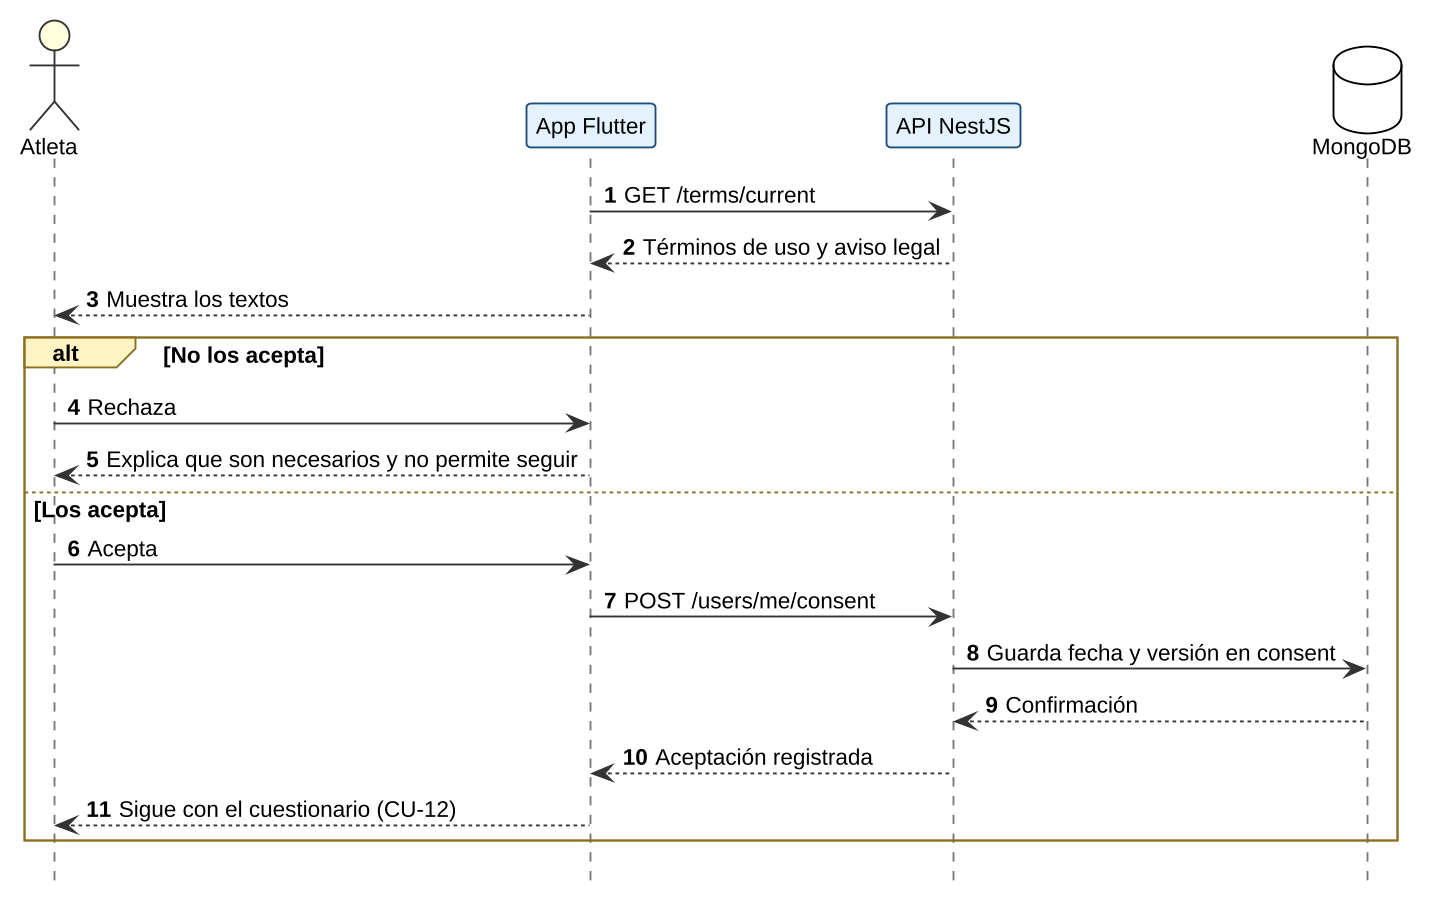
\includegraphics[width=0.95\textwidth,height=0.6\textheight,keepaspectratio]{figuras/secuencia/sec_cu26.png}
    \captionof{figure}{Diagrama de Secuencia -- CU-26: Aceptar los términos de uso y el aviso legal.}
    \label{fig:sec_cu26}
\end{center}
La aplicación pide al backend la versión vigente de los textos. Si el usuario los acepta, el backend guarda la fecha y la versión en \texttt{consent}, para poder demostrar qué aceptó. Sin esta aceptación no se puede seguir con el cuestionario inicial.
\end{minipage}
\vspace{0.6cm}

\noindent\begin{minipage}{\linewidth}
\textbf{CU-27. Crear una receta}

Para el caso de uso CU-27 se genera el diagrama de secuencia que se muestra en la Figura \ref{fig:sec_cu27}.
\begin{center}
    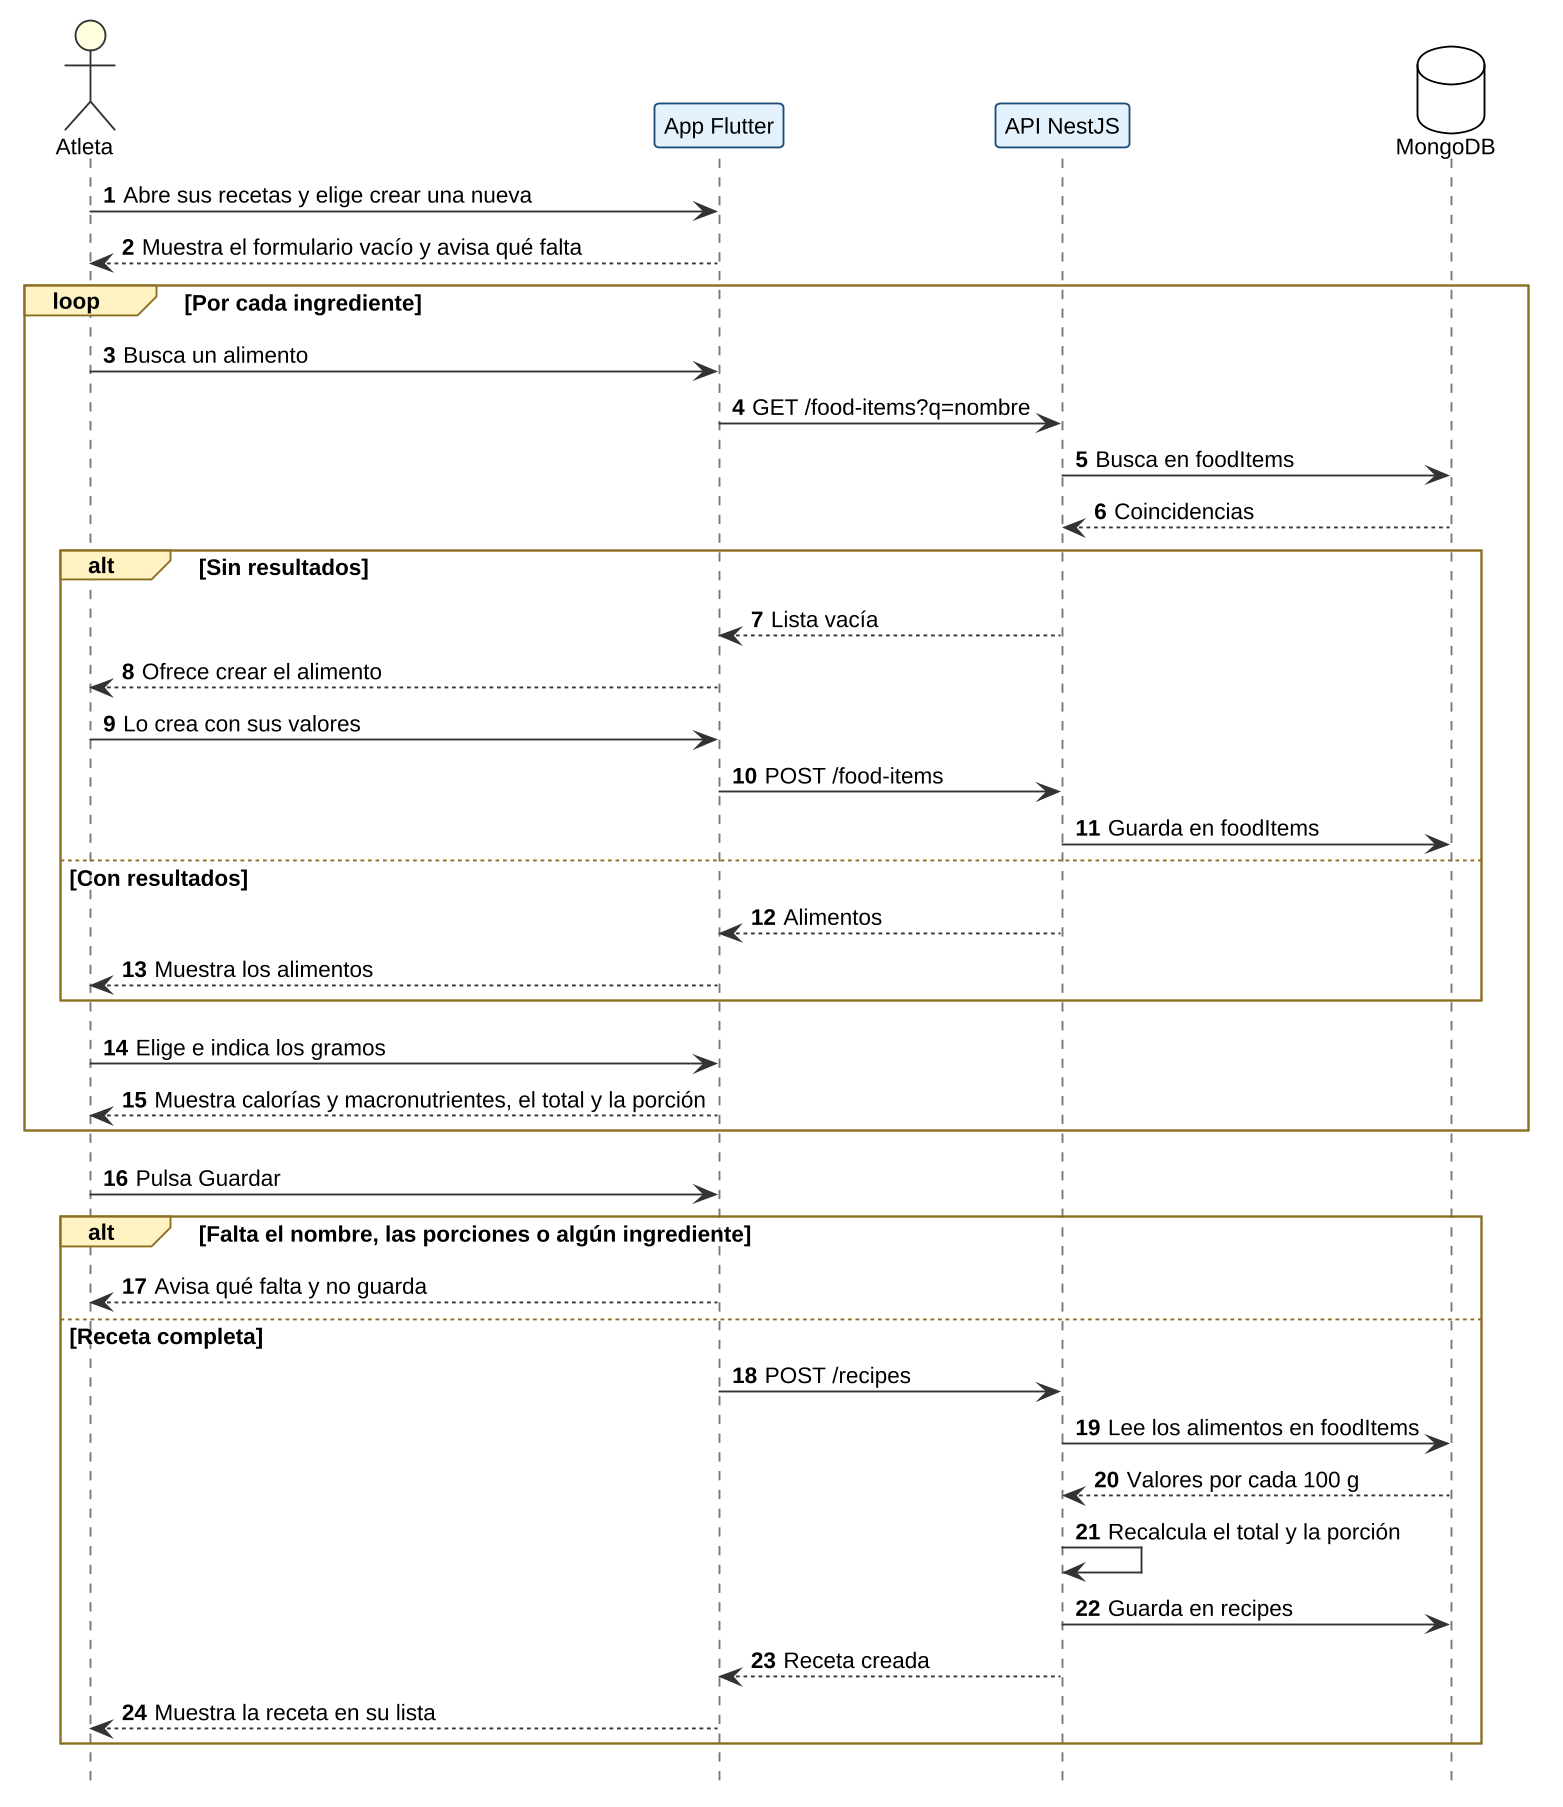
\includegraphics[width=0.95\textwidth,height=0.6\textheight,keepaspectratio]{figuras/secuencia/sec_cu27.png}
    \captionof{figure}{Diagrama de Secuencia -- CU-27: Crear una receta.}
    \label{fig:sec_cu27}
\end{center}
Por cada ingrediente, la aplicación busca en el catálogo \texttt{foodItems} a través del backend, y si el alimento no existe permite crearlo. Mientras el usuario arma la receta, la aplicación muestra los valores calculados, pero al guardar el backend los recalcula con los datos del catálogo y no confía en los que envía el teléfono. La receta se guarda en \texttt{recipes}, con su autor, y parte como privada. Si el usuario la publica después, se sigue el caso de uso CU-09.
\end{minipage}
\vspace{0.6cm}

\subsection{Diseño de Interfaces de Usuario}
En esta sección se muestran las pantallas que cubren cada caso de uso. Se construyeron en la aplicación Flutter del prototipo, y no en una herramienta de dibujo, para que el diseño sirva como base del desarrollo. El administrador usa un panel web, según lo definido en la arquitectura.

La interfaz usa Material Design 3 como base y agrega patrones de iOS, como las tarjetas agrupadas y las transiciones entre pantallas. Se organiza en cuatro módulos, que se eligen en el selector superior: nutrición, fuerza, cardio y comunidad. Cada módulo tiene sus secciones en la barra inferior. La paleta de colores es Gruvbox, con una versión clara y otra oscura, y cada macronutriente mantiene siempre su color. Las figuras de esta sección usan el modo claro, porque se lee mejor en una hoja impresa, aunque la aplicación también cuenta con el modo oscuro exigido en los requisitos de las interfaces.

\newlength{\uiancho}\setlength{\uiancho}{3.2cm}
\newlength{\uiescritorio}\setlength{\uiescritorio}{7.85cm}
\newcommand{\uifoto}[1]{\includegraphics[width=\uiancho]{figuras/interfaces/#1.jpg}}
\newcommand{\uiweb}[1]{\includegraphics[width=\uiescritorio]{figuras/interfaces/#1.jpg}}
\newcommand{\uitexto}[1]{{\setstretch{1.1}\small #1\par}}
% Cuatro pantallas: el texto va arriba.
\newcommand{\uicuatro}[8]{%
\noindent\begin{minipage}{\linewidth}
\textbf{#1}\par\vspace{0.1cm}
\uitexto{#2}\vspace{0.2cm}
\centering\uifoto{#3}\hspace{0.45cm}\uifoto{#4}\hspace{0.45cm}\uifoto{#5}\hspace{0.45cm}\uifoto{#6}
\captionof{figure}{Interfaces -- #7.}\label{#8}
\end{minipage}\par\vspace{0.3cm}}
% Tres pantallas: el texto va a la izquierda.
\newcommand{\uitres}[7]{%
\noindent\begin{minipage}{\linewidth}
\begin{minipage}[c]{5.5cm}\raggedright\textbf{#1}\par\vspace{0.15cm}\uitexto{#2}\end{minipage}\hfill
\begin{minipage}[c]{10.1cm}\uifoto{#3}\hfill\uifoto{#4}\hfill\uifoto{#5}\end{minipage}
\captionof{figure}{Interfaces -- #6.}\label{#7}
\end{minipage}\par\vspace{0.3cm}}
% Dos pantallas: el texto va a la izquierda.
\newcommand{\uidos}[6]{%
\noindent\begin{minipage}{\linewidth}
\begin{minipage}[c]{9cm}\raggedright\textbf{#1}\par\vspace{0.15cm}\uitexto{#2}\end{minipage}\hfill
\begin{minipage}[c]{6.7cm}\uifoto{#3}\hfill\uifoto{#4}\end{minipage}
\captionof{figure}{Interfaces -- #5.}\label{#6}
\end{minipage}\par\vspace{0.3cm}}
% Dos casos de uso de dos pantallas, uno al lado del otro.
\newcommand{\uipar}[6]{%
\begin{minipage}[t]{7.75cm}\raggedright\textbf{#1}\par\vspace{0.1cm}\uitexto{#2}\vspace{0.2cm}\uifoto{#3}\hspace{0.3cm}\uifoto{#4}
\captionof{figure}{Interfaces -- #5.}\label{#6}\end{minipage}}
% Dos pantallas del panel web, con el texto arriba.
\newcommand{\uiweblado}[6]{%
\noindent\begin{minipage}{\linewidth}
\textbf{#1}\par\vspace{0.1cm}
\uitexto{#2}\vspace{0.2cm}
\centering\uiweb{#3}\hfill\uiweb{#4}
\captionof{figure}{Interfaces -- #5.}\label{#6}
\end{minipage}\par\vspace{0.3cm}}

\textbf{Estado de las pantallas.} El prototipo no tiene todavía el backend ni las integraciones diseñadas en este capítulo, por lo que no todas las pantallas funcionan de la misma manera. La Tabla \ref{tab:estado_interfaces} indica cuáles ya operan y cuáles muestran datos simulados. Las pantallas simuladas siguen el flujo de su caso de uso, pero sus resultados son ejemplos fijos y no se guardan en una base de datos. Las personas que aparecen son ficticias, y los recuadros de color reemplazan a las fotos.

\begin{table}[h!]
    \centering
    \renewcommand{\arraystretch}{1.2}
    \small
    \begin{tabular}{|>{\raggedright\arraybackslash}p{3.1cm}|>{\raggedright\arraybackslash}p{4.4cm}|>{\raggedright\arraybackslash}p{7.4cm}|}
        \hline
        \rowcolor[HTML]{EFEFEF}
        \textbf{Estado} & \textbf{Casos de uso} & \textbf{Qué significa} \\ \hline
        Funcional & CU-01, CU-06, CU-15, CU-27 & La pantalla opera con su lógica real en el prototipo. \\ \hline
        Funcional en parte & CU-05, CU-12, CU-16, CU-17, CU-18, CU-19, CU-20, CU-21 & Una parte es real, como el cálculo de la carga o la grabación con GPS, y el resto se muestra con datos simulados. \\ \hline
        Diseño con datos simulados & CU-02, CU-03, CU-04, CU-07, CU-08, CU-09, CU-10, CU-11, CU-13, CU-14, CU-22, CU-23, CU-24, CU-25, CU-26 & La pantalla muestra el flujo completo, pero falta conectar el servicio que la sostiene, como la IA, los pagos, la red social o la lectura del reloj. \\ \hline
    \end{tabular}
    \caption{Estado de las pantallas en el prototipo.}
    \label{tab:estado_interfaces}
\end{table}

Cada figura se lee de izquierda a derecha, siguiendo el curso normal del caso de uso y, cuando corresponde, alguno de sus cursos alternos.
\vspace{0.3cm}

\uicuatro{CU-01. Anotar una sesión de fuerza}{Desde el módulo de fuerza, el atleta empieza una rutina guardada o una sesión libre. Durante la sesión anota el peso y las repeticiones de cada serie. Al terminar indica qué tan duro lo sintió, y la aplicación muestra el resumen con su carga.}{cu01_inicio}{cu01_entreno}{cu01_esfuerzo}{cu01_detalle}{CU-01: Anotar una sesión de fuerza}{fig:ui_cu01}

\noindent\uipar{CU-02. Contar mi sesión de fuerza con mis palabras}{El atleta escribe o dicta lo que hizo. El asistente lo ordena en ejercicios y series. Si no reconoce un ejercicio, lo marca y no deja guardar hasta que se elija de la lista.}{cu02_escribir}{cu02_revision}{CU-02: Contar mi sesión de fuerza con mis palabras}{fig:ui_cu02}\hfill
\uipar{CU-03. Traer mis sesiones desde el reloj}{La primera vez se explica para qué se usan los datos y se pide permiso. Luego las sesiones nuevas llegan solas, y se pregunta qué tan duro se sintió cada una.}{cu03_permiso}{cu03_sesiones}{CU-03: Traer mis sesiones desde el reloj}{fig:ui_cu03}
\par\vspace{0.3cm}

\uitres{CU-04. Subir el archivo de mi ciclocomputador}{El atleta elige un archivo \texttt{.fit} de hasta 10 MB. Si el archivo no sirve, se explica el motivo. Si es válido, se muestra la sesión con su potencia, su cadencia y su pulso antes de guardarla.}{cu04_elegir}{cu04_error}{cu04_resumen}{CU-04: Subir el archivo de mi ciclocomputador}{fig:ui_cu04}

\uitres{CU-05. Revisar mi fatiga y recibir alertas}{El resumen suma la carga de fuerza y de cardio en una misma unidad. Si detecta un riesgo, muestra un aviso con una sugerencia que el atleta decide si sigue. Con pocas sesiones, avisa que faltan datos. La carga ya se calcula con los registros reales, y la alerta es un ejemplo.}{cu05_resumen}{cu05_alerta}{cu05_faltan}{CU-05: Revisar mi fatiga y recibir alertas}{fig:ui_cu05}

\uitres{CU-06. Anotar una comida buscando los alimentos}{El diario muestra el avance del día. En Registrar, el usuario elige los alimentos y sus cantidades, y la aplicación calcula las calorías y los macronutrientes. El catálogo reúne los alimentos disponibles.}{cu06_diario}{cu06_registrar}{cu06_catalogo}{CU-06: Anotar una comida buscando los alimentos}{fig:ui_cu06}

\uitres{CU-07. Registrar una comida con una foto}{El atleta saca la foto y el asistente estima los alimentos y sus cantidades. Lo que no es seguro queda marcado para revisarlo. La foto se descarta al guardar, salvo que el atleta decida publicarla.}{cu07_camara}{cu07_analizando}{cu07_revision}{CU-07: Registrar una comida con una foto}{fig:ui_cu07}

\uitres{CU-08. Agregar una receta ajustada a mis metas}{Desde la receta, la aplicación calcula lo que le falta comer al usuario y ajusta todos los ingredientes con un mismo factor, que se puede cambiar. Si ya cumplió sus metas, lo avisa y propone las porciones originales.}{cu08_receta}{cu08_ajuste}{cu08_metas}{CU-08: Agregar una receta ajustada a mis metas}{fig:ui_cu08}

\uitres{CU-09. Publicar una sesión, ruta o comida}{El atleta elige un registro (una sesión, una ruta, una comida o una receta que creó), escribe un texto y decide quién lo puede ver. Puede agregar hasta 4 fotos, y para eso debe declarar que son suyas o que tiene permiso. Si publica una ruta, la aplicación oculta el inicio y el final del recorrido. Una receta se publica con sus ingredientes.}{cu09_sesion}{cu09_ruta}{cu09_receta}{CU-09: Publicar una sesión, ruta o comida}{fig:ui_cu09}

\uiweblado{CU-10. Mantener el catálogo de ejercicios}{En el panel web, el administrador revisa la lista, agrega o cambia ejercicios y puede desactivarlos. Un ejercicio desactivado deja de aparecer para nuevas sesiones. Si el nombre ya existe, el panel lo avisa y no permite guardar.}{cu10_lista}{cu10_repetido}{CU-10: Mantener el catálogo de ejercicios}{fig:ui_cu10}

\uiweblado{CU-11. Revisar el contenido reportado}{El administrador ve las publicaciones reportadas con su motivo. Al revisar una, debe explicar su decisión antes de ocultarla o de descartar el reporte, y queda guardado quién la tomó y por qué.}{cu11_lista}{cu11_revisar}{CU-11: Revisar el contenido reportado}{fig:ui_cu11}

\uicuatro{CU-12. Completar mi perfil y recibir un plan semanal}{El cuestionario inicial se responde en tres pasos: experiencia y objetivo, disponibilidad y equipamiento, y datos personales. Con eso, la aplicación sugiere un plan para la semana, que el usuario puede aceptar, cambiar o dejar para después.}{cu12_cuestionario1}{cu12_cuestionario2}{cu12_cuestionario3}{cu12_plan}{CU-12: Completar mi perfil y recibir un plan semanal}{fig:ui_cu12}

\uitres{CU-13. Agregar una publicación a mis módulos}{Desde una publicación, el atleta revisa qué se va a agregar y quién lo creó. Al confirmar, queda una copia propia en el módulo que corresponde, que puede cambiar sin afectar la original.}{cu13_publicacion}{cu13_agregar}{cu13_listo}{CU-13: Agregar una publicación a mis módulos}{fig:ui_cu13}

\noindent\uipar{CU-14. Seguir a otro usuario}{El atleta busca a una persona por nombre o deporte, abre su perfil y la sigue. Puede dejar de seguirla con el mismo botón.}{cu14_buscar}{cu14_perfil}{CU-14: Seguir a otro usuario}{fig:ui_cu14}\hfill
\uipar{CU-15. Registrar un producto con su código de barras}{El usuario escanea el producto o escribe el código, y luego ajusta la porción. La imagen del visor es de ejemplo, porque el simulador no tiene cámara.}{cu15_escaner}{cu15_porcion}{CU-15: Registrar un producto con su código de barras}{fig:ui_cu15}
\par\vspace{0.3cm}

\uidos{CU-16. Contar mi comida con mis palabras}{El atleta escribe o dicta lo que comió. El asistente estima los alimentos y sus cantidades, y lo que no es seguro queda marcado. El usuario corrige los gramos o quita un alimento antes de guardarlo en su diario.}{cu16_escribir}{cu16_revision}{CU-16: Contar mi comida con mis palabras}{fig:ui_cu16}

\uicuatro{CU-17. Registrar una sesión de cardio sin reloj}{El usuario elige la disciplina y graba con un solo toque. Durante la salida ve el tiempo, las métricas y el mapa. Al terminar indica qué tan dura la sintió. Si no quiere usar el GPS, puede anotar la sesión a mano.}{cu17_inicio}{cu17_grabar}{cu17_guardar}{cu17_manual}{CU-17: Registrar una sesión de cardio sin reloj}{fig:ui_cu17}

\uidos{CU-18. Ver mis metas de alimentación del día}{El resumen muestra las metas según el entrenamiento del día, cuánto falta y en qué momento conviene comer. Un día de descanso muestra metas distintas. Son sugerencias y no una dieta. El avance del día es real, y el ajuste de las metas es un ejemplo.}{cu18_entreno}{cu18_descanso}{CU-18: Ver mis metas de alimentación del día}{fig:ui_cu18}

\uitres{CU-19. Revisar mi progreso}{El calendario muestra por día y por mes las comidas y los entrenamientos. La carga muestra cómo ha cambiado en el tiempo, y el progreso corporal muestra la tendencia del peso hacia la meta.}{cu19_calendario}{cu19_carga}{cu19_progreso}{CU-19: Revisar mi progreso}{fig:ui_cu19}

\uidos{CU-20. Anotar cómo me sentí}{Al abrir un entrenamiento o una comida, el usuario escribe cómo se sintió y la nota queda junto a ese registro. Si pulsa Guardar sin escribir nada, no se crea ninguna nota.}{cu20_sesion}{cu20_comida}{CU-20: Anotar cómo me sentí}{fig:ui_cu20}

\uitres{CU-21. Controlar mis datos personales}{Desde los ajustes, el usuario revisa y corrige sus datos, y decide qué permisos entrega. Para eliminar su cuenta debe confirmarlo escribiendo una palabra, y antes se le explica qué se borrará.}{cu21_ajustes}{cu21_datos}{cu21_eliminar}{CU-21: Controlar mis datos personales}{fig:ui_cu21}

\noindent\uipar{CU-22. Reportar una publicación}{El atleta elige un motivo y envía el reporte, o cancela sin enviar nada. La publicación pasa a revisión y deja de aparecer en su muro.}{cu22_motivo}{cu22_listo}{CU-22: Reportar una publicación}{fig:ui_cu22}\hfill
\uipar{CU-23. Ver el muro de la comunidad}{El muro reúne las publicaciones recientes de las personas que sigue. Desde cada una se puede abrir el detalle, agregarla a los módulos o reportarla.}{cu23_muro}{cu23_ruta}{CU-23: Ver el muro de la comunidad}{fig:ui_cu23}
\par\vspace{0.3cm}

\noindent\uipar{CU-24. Contratar el plan premium}{La pantalla muestra qué incluye cada plan, el precio final con IVA y cada cuánto se cobra. Al confirmar se abre el pago de la tienda y se activan las funciones.}{cu24_planes}{cu24_activo}{CU-24: Contratar el plan premium}{fig:ui_cu24}\hfill
\uipar{CU-25. Cancelar mi suscripción}{El usuario ve su plan y la fecha del próximo cobro. La cancelación se confirma en la tienda, y mantiene el plan premium hasta que termina el periodo pagado.}{cu25_activa}{cu25_cancelada}{CU-25: Cancelar mi suscripción}{fig:ui_cu25}
\par\vspace{0.3cm}

\uidos{CU-26. Aceptar los términos de uso y el aviso legal}{Al crear su cuenta, el usuario lee los términos y los acepta para continuar. Si no los acepta, la aplicación explica que son necesarios y no permite seguir. Si cambian más adelante, se vuelven a mostrar.}{cu26_terminos}{cu26_rechazo}{CU-26: Aceptar los términos de uso y el aviso legal}{fig:ui_cu26}

\uicuatro{CU-27. Crear una receta}{El usuario abre el formulario de una receta nueva, que le avisa qué falta para poder guardarla. Agrega cada ingrediente desde el catálogo de alimentos e indica sus gramos, y la aplicación calcula el total y lo que aporta cada porción. Al guardarla, la receta aparece en su lista de recetas, donde la puede buscar al registrar una comida. Estas pantallas son las del prototipo y operan con su lógica real.}{cu27_nueva}{cu27_ingredientes}{cu27_completa}{cu27_lista}{CU-27: Crear una receta}{fig:ui_cu27}

\subsection{Diagrama de Integraciones}
La solución se conecta con seis sistemas que no son parte del proyecto. La Figura \ref{fig:diagrama_integraciones} muestra estas integraciones y desde dónde se usa cada una. Hay una regla general: las claves de acceso a los servicios externos se guardan solo en el backend y nunca en la aplicación, porque cualquier persona podría extraerlas del teléfono. Por eso, las únicas conexiones que parten desde la aplicación son las que no necesitan una clave secreta o las que usan un permiso temporal.
\begin{center}
    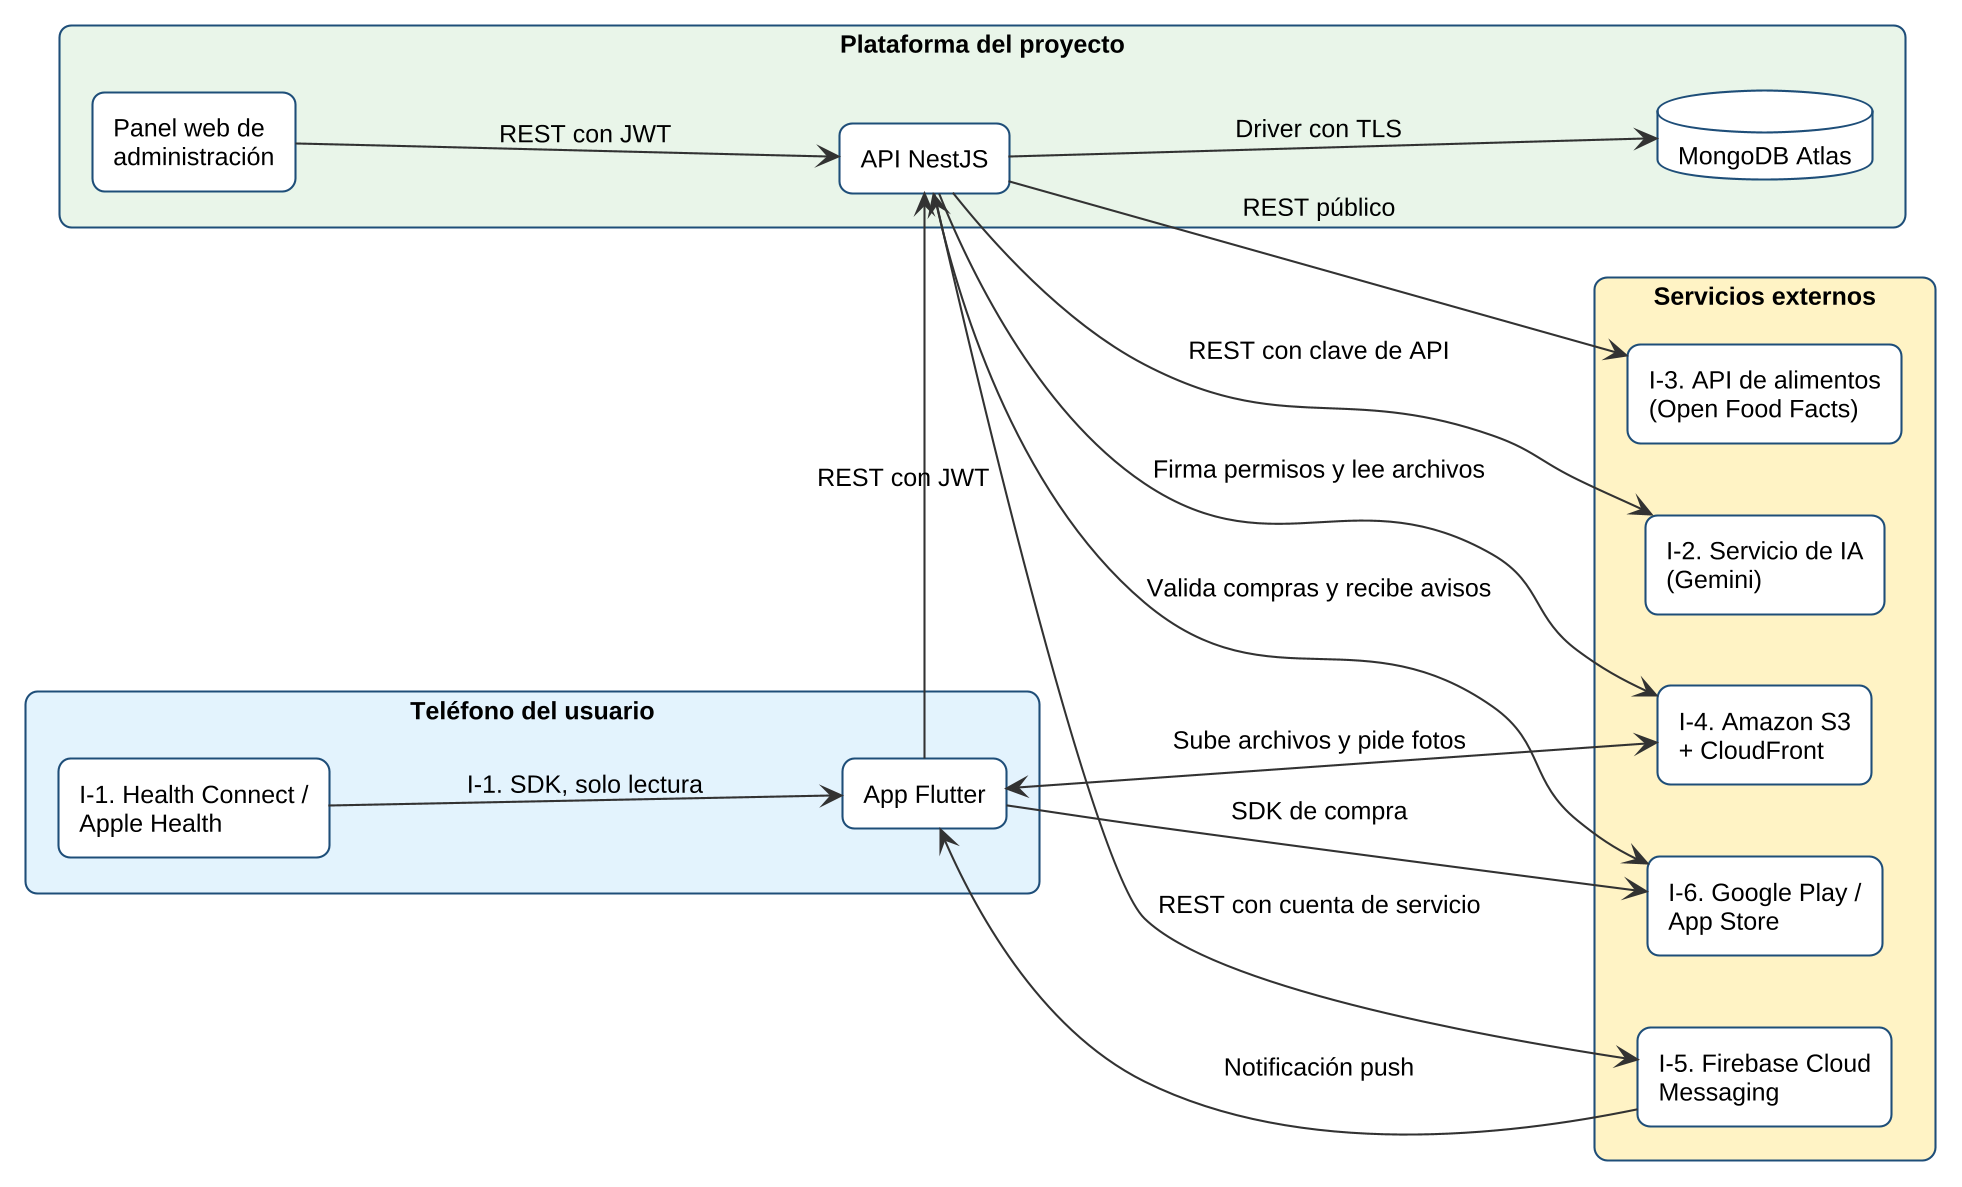
\includegraphics[width=1\textwidth,height=0.5\textheight,keepaspectratio]{figuras/arquitectura/diagrama_integraciones.png}
    \captionof{figure}{Diagrama general de integraciones.}
    \label{fig:diagrama_integraciones}
\end{center}

La Tabla \ref{tab:integraciones} resume cada integración y lo que ocurre cuando el sistema externo falla. Ninguna falla externa debería impedir que el usuario siga registrando sus datos a mano.

\begin{table}[h!]
    \centering
    \renewcommand{\arraystretch}{1.25}
    \footnotesize
    \begin{tabular}{|p{0.7cm}|>{\raggedright\arraybackslash}p{2.6cm}|>{\raggedright\arraybackslash}p{3.8cm}|>{\raggedright\arraybackslash}p{3.3cm}|>{\raggedright\arraybackslash}p{3.8cm}|}
        \hline
        \rowcolor[HTML]{EFEFEF}
        \textbf{ID} & \textbf{Sistema} & \textbf{Para qué se usa} & \textbf{Cómo se conecta} & \textbf{Si falla} \\ \hline
        I-1 & Health Connect y Apple Health & Leer las sesiones de cardio del reloj (CU-03, CU-21) & SDK en el teléfono, solo lectura, con permiso del usuario & La sesión se puede registrar con el GPS o a mano (CU-17) \\ \hline
        I-2 & Servicio de IA (Gemini) & Entender fotos de comida y textos (CU-02, CU-07, CU-16) & REST desde el backend, con clave de API & Se ofrece el registro manual (CU-01 y CU-06) \\ \hline
        I-3 & API de alimentos (Open Food Facts) & Buscar productos por código de barras (CU-15) & REST público desde el backend & Se ofrece buscar el alimento en la lista (CU-06) \\ \hline
        I-4 & Amazon S3 y CloudFront & Guardar y mostrar fotos y archivos \texttt{.fit} (CU-04, CU-09, CU-23) & Subida con URL prefirmada y lectura por CloudFront & Se avisa al usuario y se conserva lo escrito para reintentar \\ \hline
        I-5 & Firebase Cloud Messaging & Enviar alertas de fatiga al teléfono (CU-05) & REST desde el backend, con cuenta de servicio & La alerta queda visible en el resumen de la aplicación \\ \hline
        I-6 & Google Play y App Store & Cobrar y cancelar la suscripción (CU-24, CU-25) & SDK de compra en el teléfono y API de la tienda en el backend & No se activa el plan premium hasta confirmar el pago \\ \hline
    \end{tabular}
    \caption{Resumen de las integraciones con sistemas externos.}
    \label{tab:integraciones}
\end{table}
A continuación se presenta el diseño de cada integración, indicando los datos que se envían y se reciben en cada mensaje.
\vspace{0.4cm}

\noindent\begin{minipage}{\linewidth}
\textbf{I-1. Health Connect y Apple Health}

La Figura \ref{fig:int_salud} muestra la lectura de las sesiones que registró el reloj.
\begin{center}
    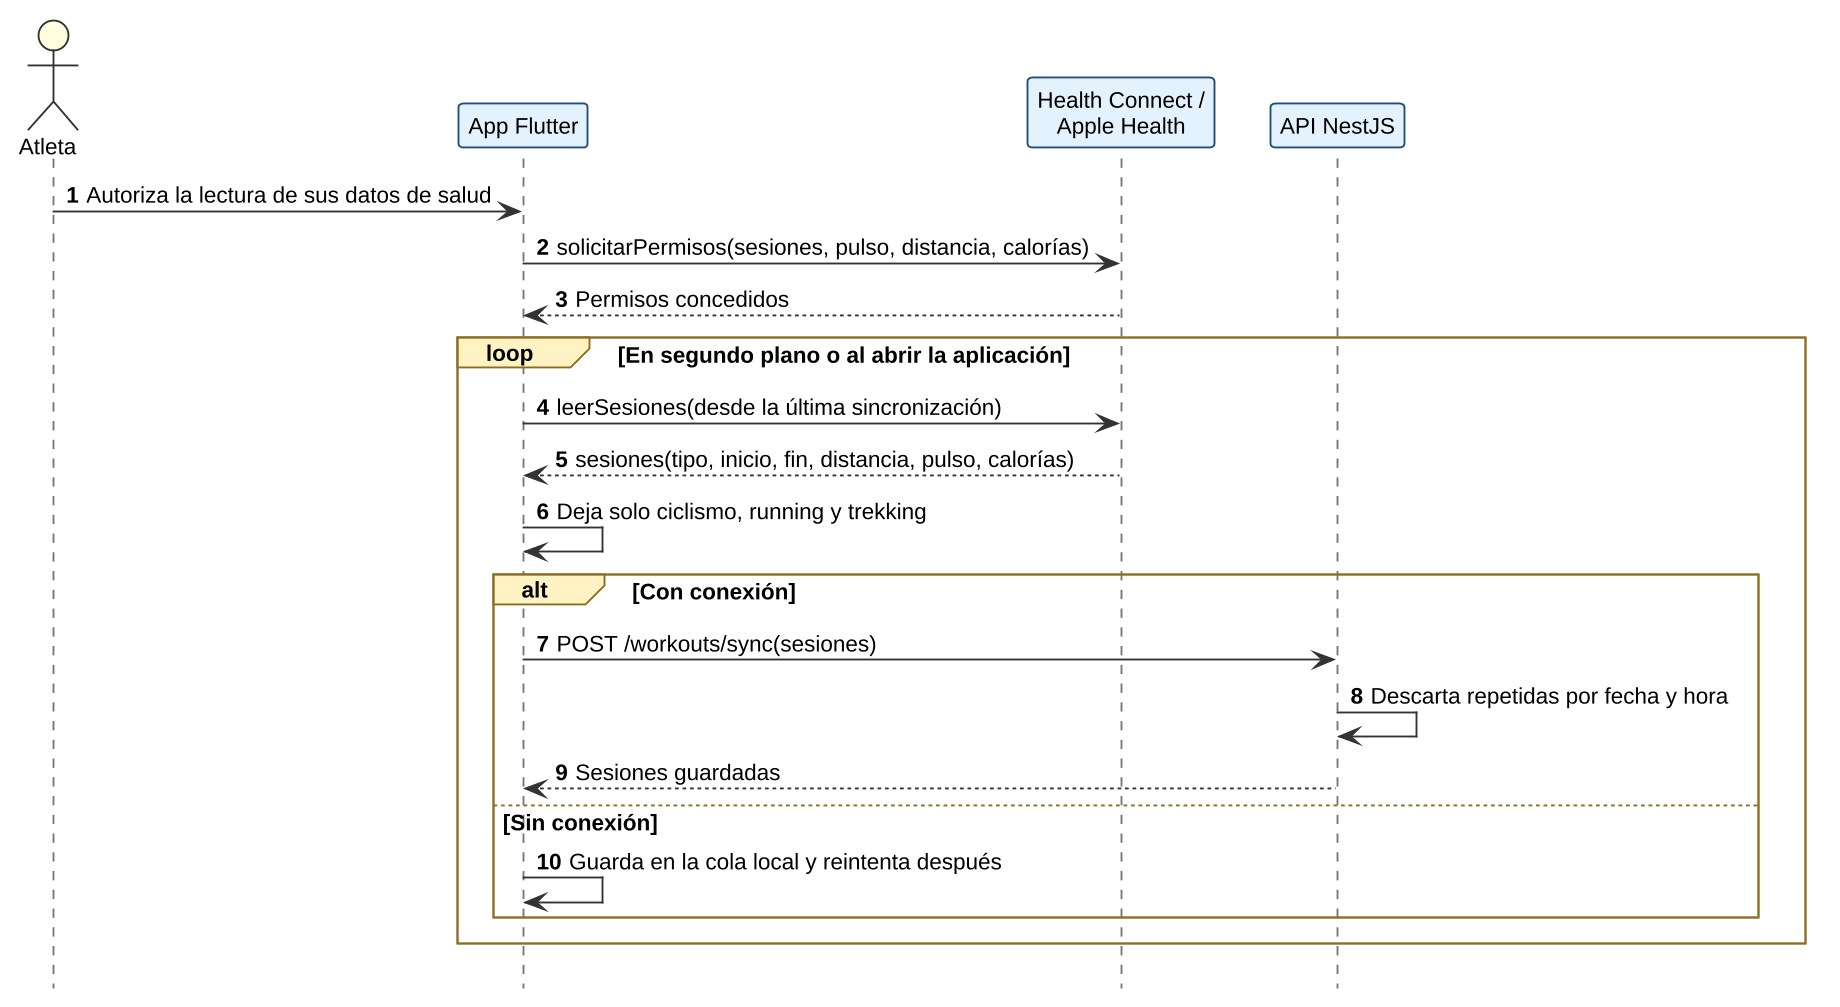
\includegraphics[width=0.95\textwidth,height=0.5\textheight,keepaspectratio]{figuras/secuencia/int_salud.png}
    \captionof{figure}{Integración I-1: Health Connect y Apple Health.}
    \label{fig:int_salud}
\end{center}
Estos servicios funcionan dentro del teléfono y no tienen una conexión directa con el servidor, por lo que la lectura la hace la aplicación con sus SDK. Solo se pide permiso para los datos necesarios, y el usuario puede retirarlo cuando quiera (CU-21). La integración es solo de lectura. Si no hay conexión, las sesiones esperan en una cola local. El backend descarta las repetidas según su fecha y hora, y conserva la versión con más detalle si la misma sesión llegó en un archivo \texttt{.fit}.
\end{minipage}
\vspace{0.6cm}

\noindent\begin{minipage}{\linewidth}
\textbf{I-2. Servicio de inteligencia artificial}

La Figura \ref{fig:int_ia} muestra cómo se estima una comida a partir de una foto o de un texto. El registro de fuerza por lenguaje natural usa el mismo esquema.
\begin{center}
    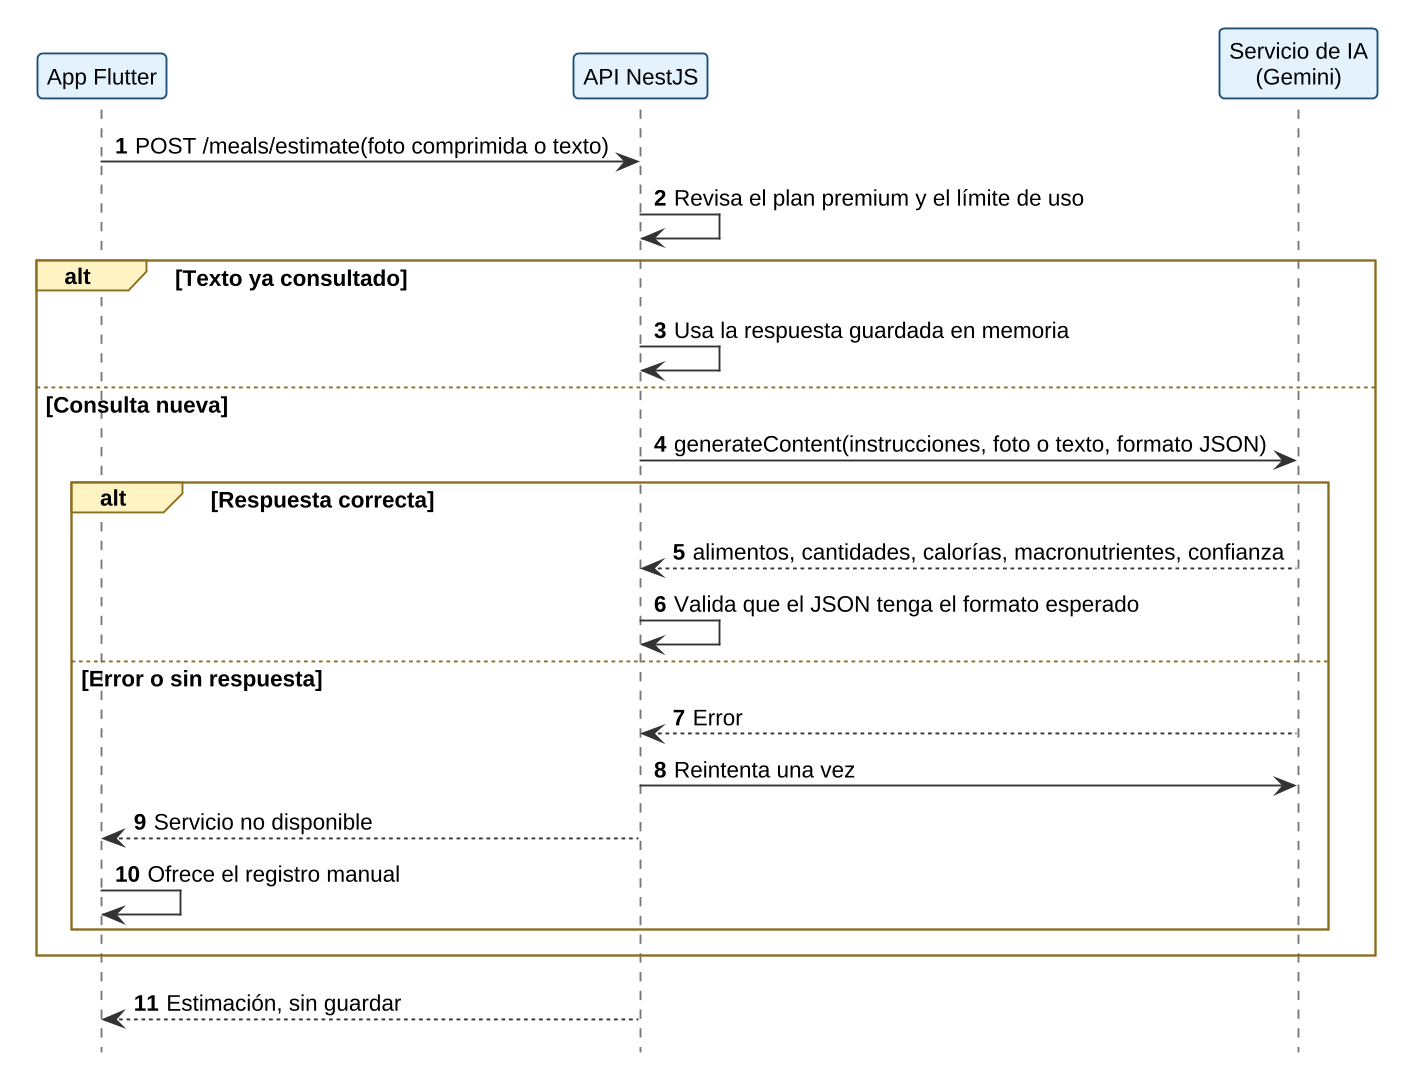
\includegraphics[width=0.95\textwidth,height=0.5\textheight,keepaspectratio]{figuras/secuencia/int_ia.png}
    \captionof{figure}{Integración I-2: Servicio de inteligencia artificial.}
    \label{fig:int_ia}
\end{center}
La aplicación nunca llama directamente al servicio de IA, para no exponer la clave y para poder controlar el gasto. El backend revisa primero el plan del usuario y su límite de uso. Solo envía la foto o el texto, sin datos que identifiquen a la persona. Como la respuesta viene de un modelo, el backend valida que el JSON tenga el formato esperado, y el usuario siempre revisa el resultado antes de guardarlo. Si se quisiera cambiar de proveedor, solo cambiaría esta integración.
\end{minipage}
\vspace{0.6cm}

\noindent\begin{minipage}{\linewidth}
\textbf{I-3. API de alimentos}

La Figura \ref{fig:int_alimentos} muestra la búsqueda de un producto por su código de barras.
\begin{center}
    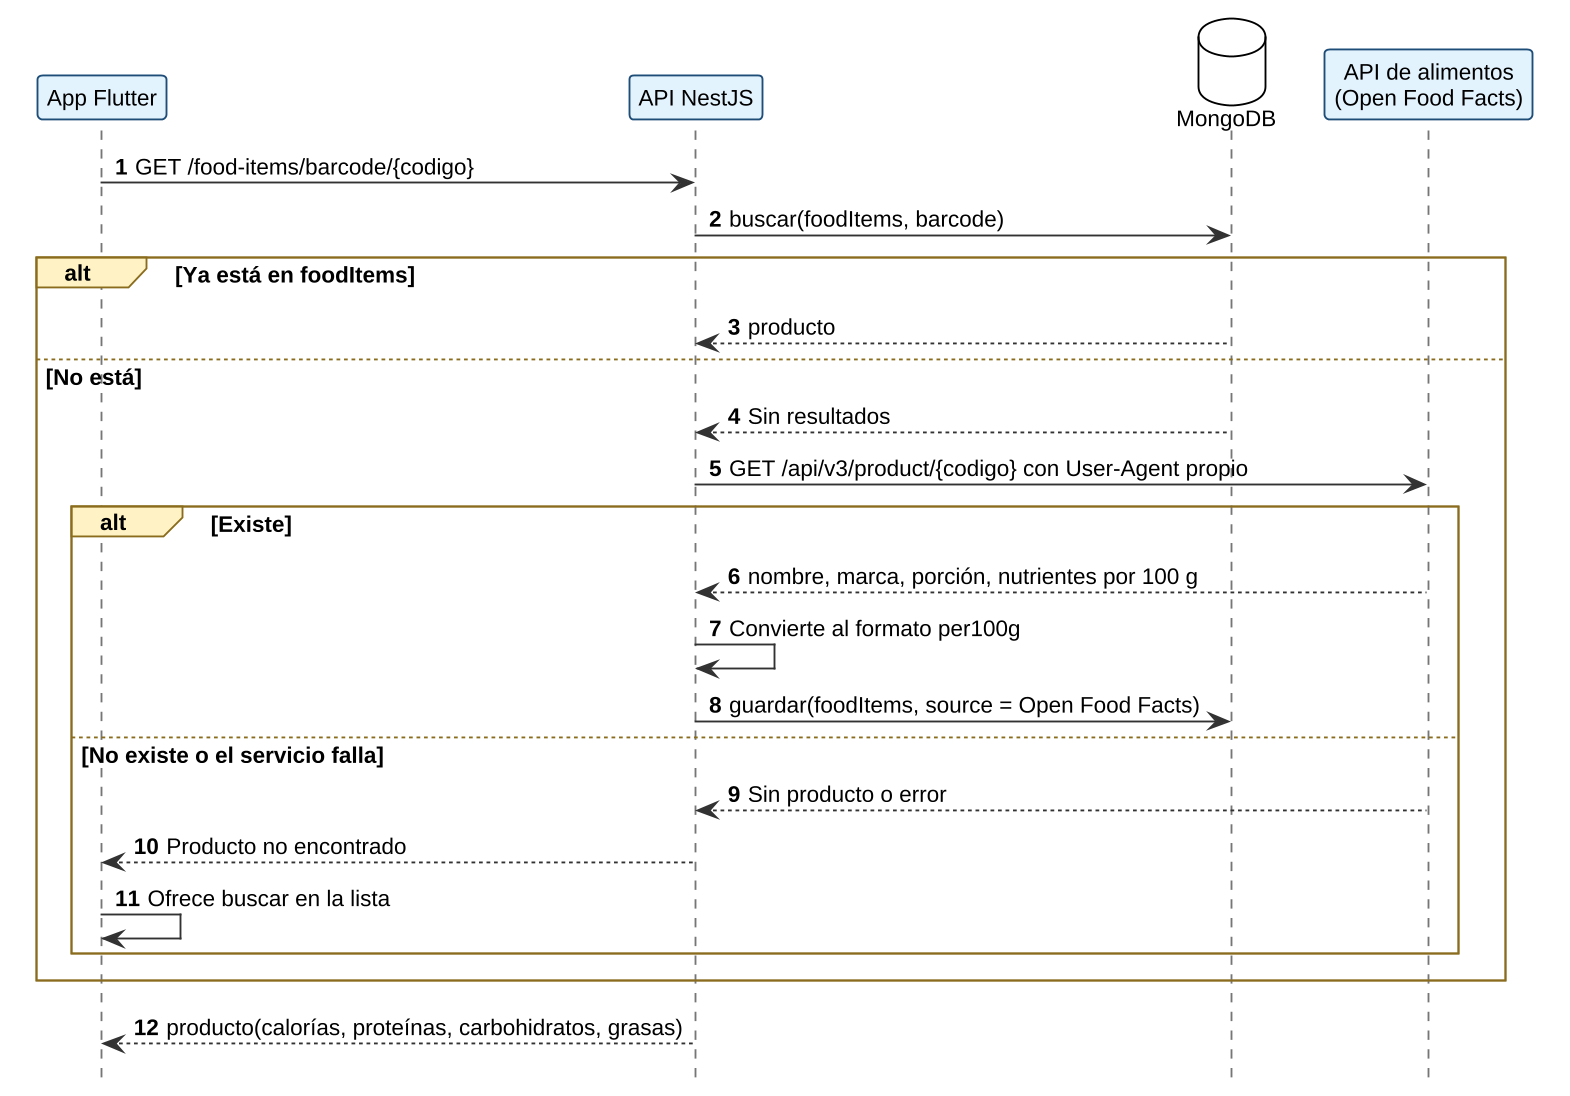
\includegraphics[width=0.95\textwidth,height=0.5\textheight,keepaspectratio]{figuras/secuencia/int_alimentos.png}
    \captionof{figure}{Integración I-3: API de alimentos.}
    \label{fig:int_alimentos}
\end{center}
Se usa la API de Open Food Facts, que para leer datos no pide autenticación, pero sí un identificador propio de la aplicación en cada consulta \citep{off_api}. Cada producto encontrado se guarda en \texttt{foodItems}, para que la siguiente consulta sea más rápida y no dependa del servicio. La licencia de estos datos (ODbL) exige indicar su origen y compartir en las mismas condiciones las bases de datos derivadas \citep{off_api}. Por eso cada producto queda marcado con su fuente en el campo \texttt{source} y la aplicación mostrará la atribución.
\end{minipage}
\vspace{0.6cm}

\noindent\begin{minipage}{\linewidth}
\textbf{I-4. Almacenamiento de archivos}

La Figura \ref{fig:int_archivos} muestra cómo se suben y se muestran las fotos de una publicación.
\begin{center}
    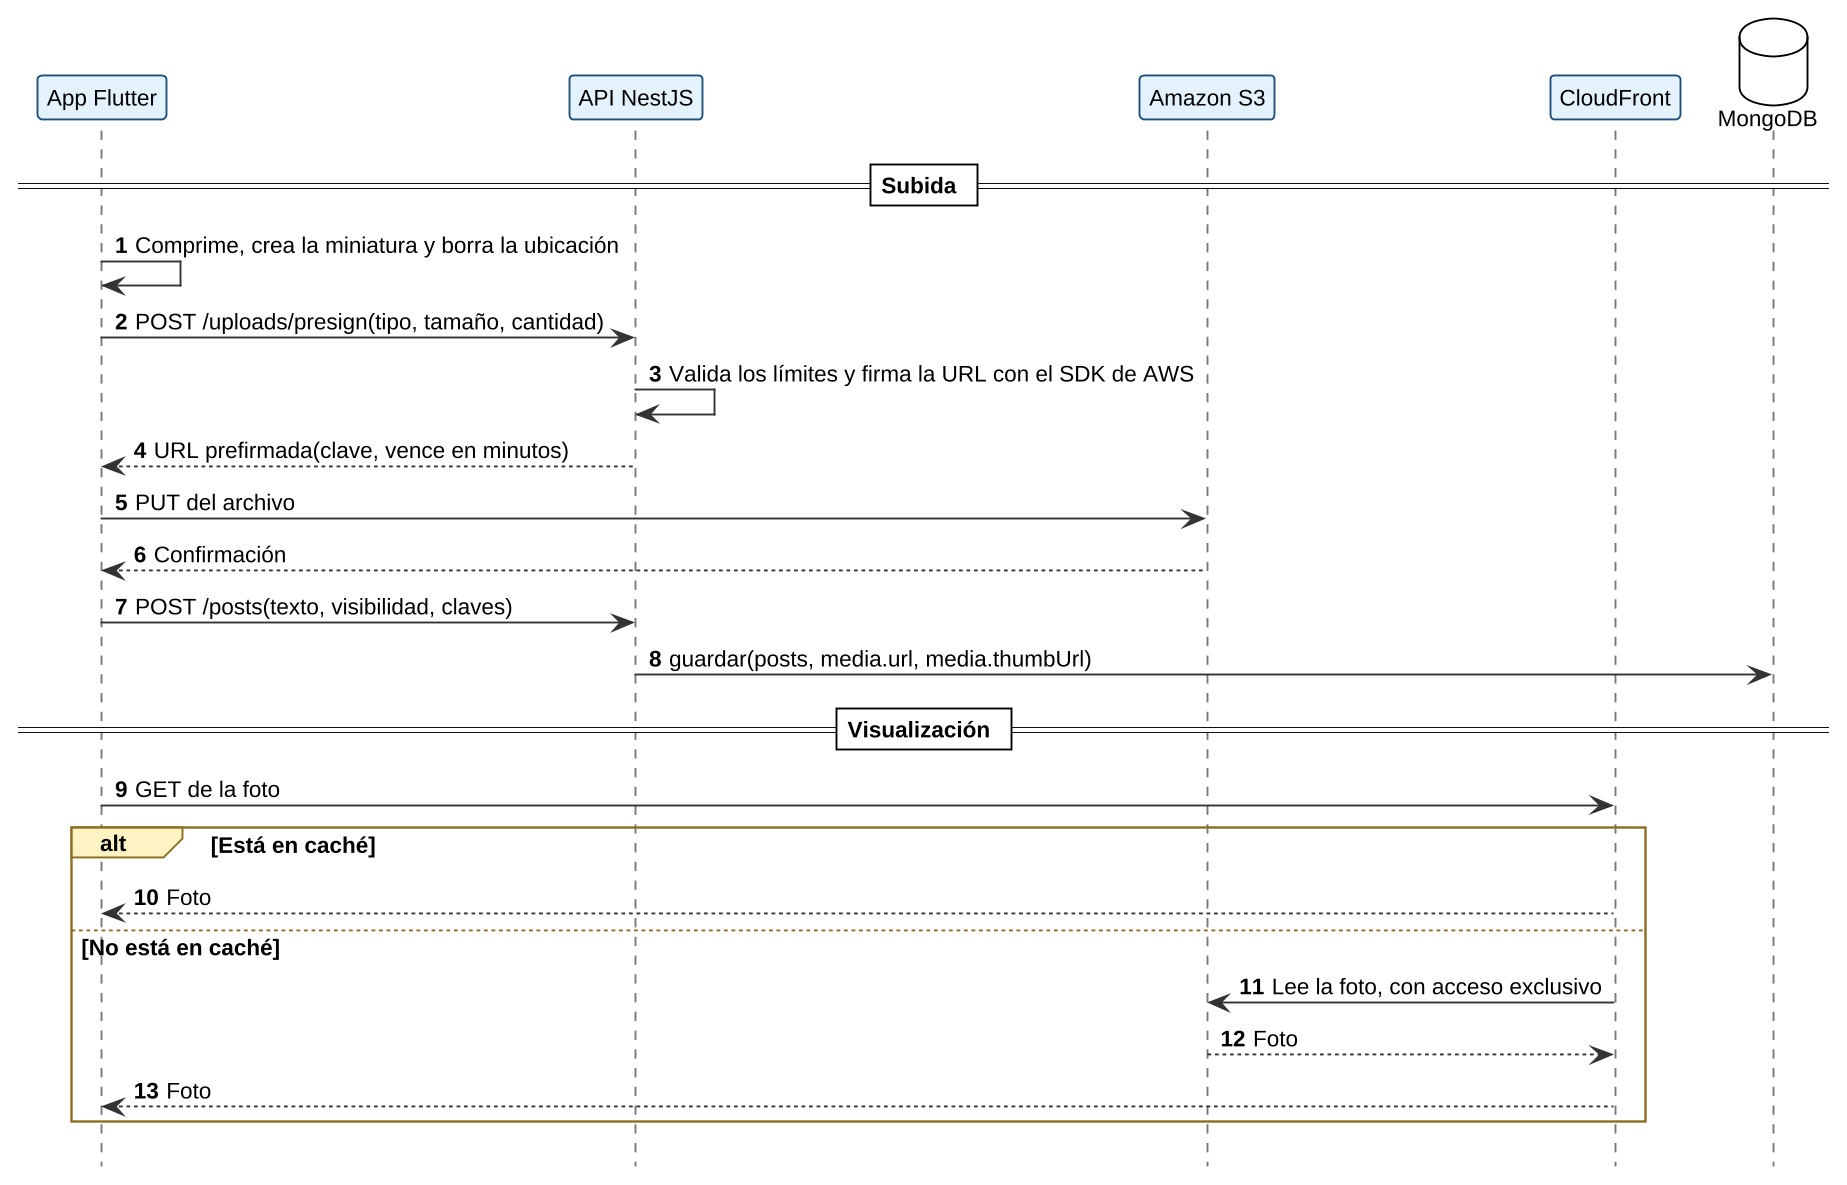
\includegraphics[width=0.95\textwidth,height=0.5\textheight,keepaspectratio]{figuras/secuencia/int_archivos.png}
    \captionof{figure}{Integración I-4: Almacenamiento de archivos.}
    \label{fig:int_archivos}
\end{center}
El teléfono sube los archivos directamente a Amazon S3 con una URL prefirmada, que vence en pocos minutos y sirve solo para ese archivo. Firmar la URL no requiere una llamada a S3, porque el backend lo hace con sus credenciales. Las fotos se muestran a través de CloudFront, que es el único servicio con permiso para leer el bucket. Los archivos \texttt{.fit} se suben igual, pero no pasan por CloudFront, porque solo los lee el backend (CU-04).
\end{minipage}
\vspace{0.6cm}

\noindent\begin{minipage}{\linewidth}
\textbf{I-5. Notificaciones}

La Figura \ref{fig:int_notificaciones} muestra el registro del teléfono y el envío de una alerta.
\begin{center}
    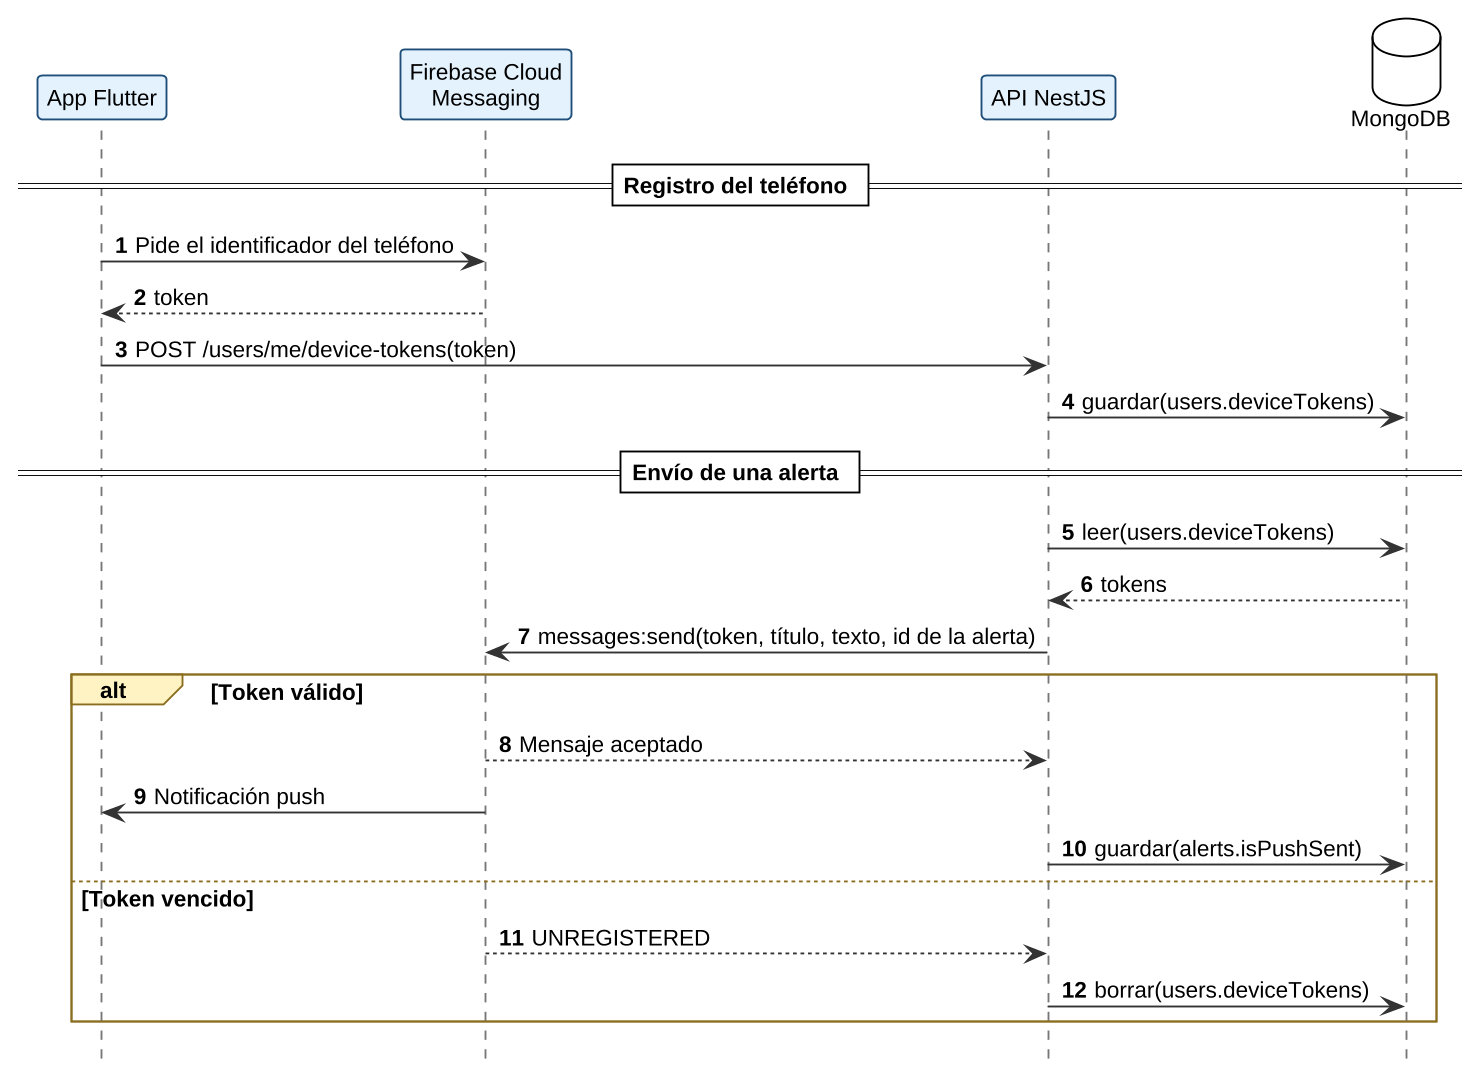
\includegraphics[width=0.95\textwidth,height=0.5\textheight,keepaspectratio]{figuras/secuencia/int_notificaciones.png}
    \captionof{figure}{Integración I-5: Notificaciones.}
    \label{fig:int_notificaciones}
\end{center}
Para enviar una notificación se necesita el identificador del teléfono, que la aplicación obtiene de Firebase y entrega al backend. Un usuario puede tener más de un teléfono, por lo que se guarda en la lista \texttt{deviceTokens}. Si Firebase responde que un identificador ya no sirve, el backend lo borra. La notificación solo es un aviso, ya que la alerta queda guardada en \texttt{fatigueSnapshots}. Así, el usuario puede verla aunque la notificación no le llegue.
\end{minipage}
\vspace{0.6cm}

\noindent\begin{minipage}{\linewidth}
\textbf{I-6. Google Play y App Store}

La Figura \ref{fig:int_pagos} muestra la compra de la suscripción y sus cambios posteriores.
\begin{center}
    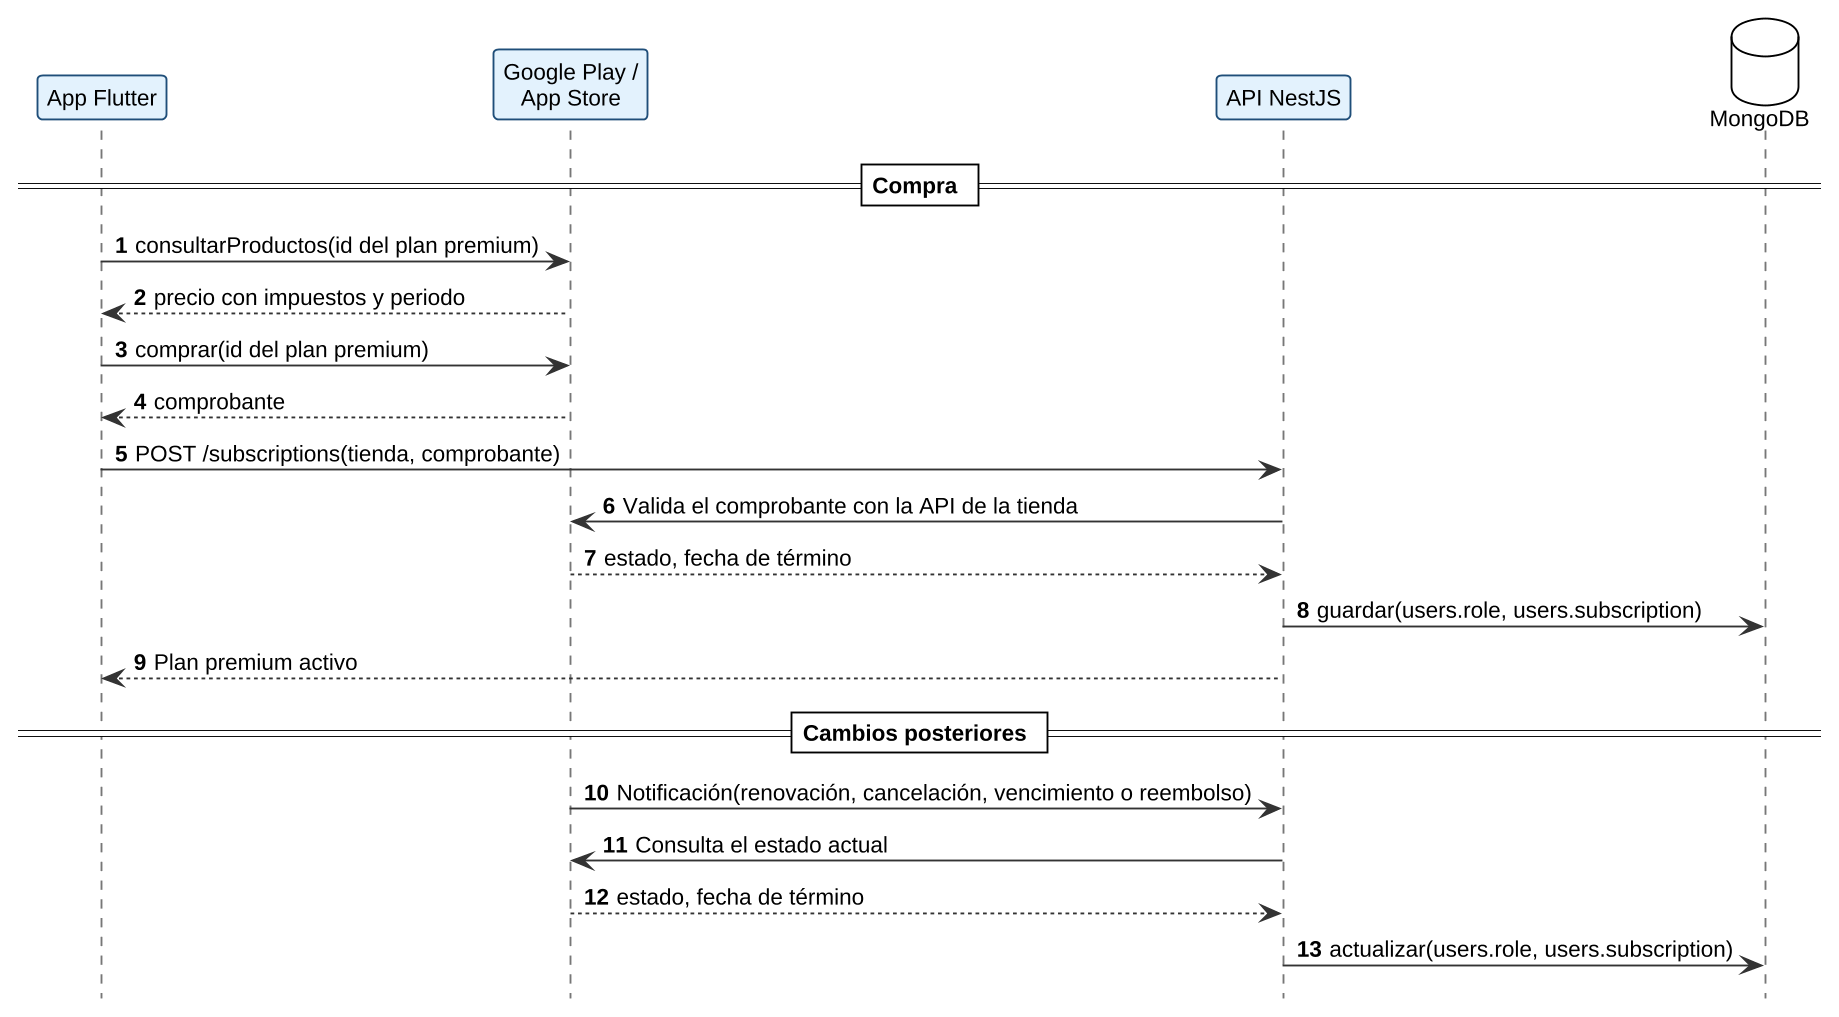
\includegraphics[width=0.95\textwidth,height=0.5\textheight,keepaspectratio]{figuras/secuencia/int_pagos.png}
    \captionof{figure}{Integración I-6: Google Play y App Store.}
    \label{fig:int_pagos}
\end{center}
El pago se hace completo en la tienda, por lo que el sistema nunca recibe los datos de la tarjeta. El backend no confía solo en lo que informa la aplicación, sino que valida cada comprobante con la API de la tienda antes de activar el plan. Las renovaciones, cancelaciones y reembolsos ocurren fuera de la aplicación, así que la tienda avisa al backend. Como ese aviso solo indica que algo cambió, el backend consulta después el estado actual \citep{google_play_rtdn}.
\end{minipage}
\vspace{0.6cm}

\subsection{Dimensionamiento y Arquitectura Detallada de la Solución}
Esta sección indica qué infraestructura se necesita para operar el MVP y cuánta capacidad debe tener. El cálculo usa como base los 1.500 usuarios del mercado objetivo inicial. La Figura \ref{fig:arquitectura_detallada} muestra la arquitectura.
\begin{center}
    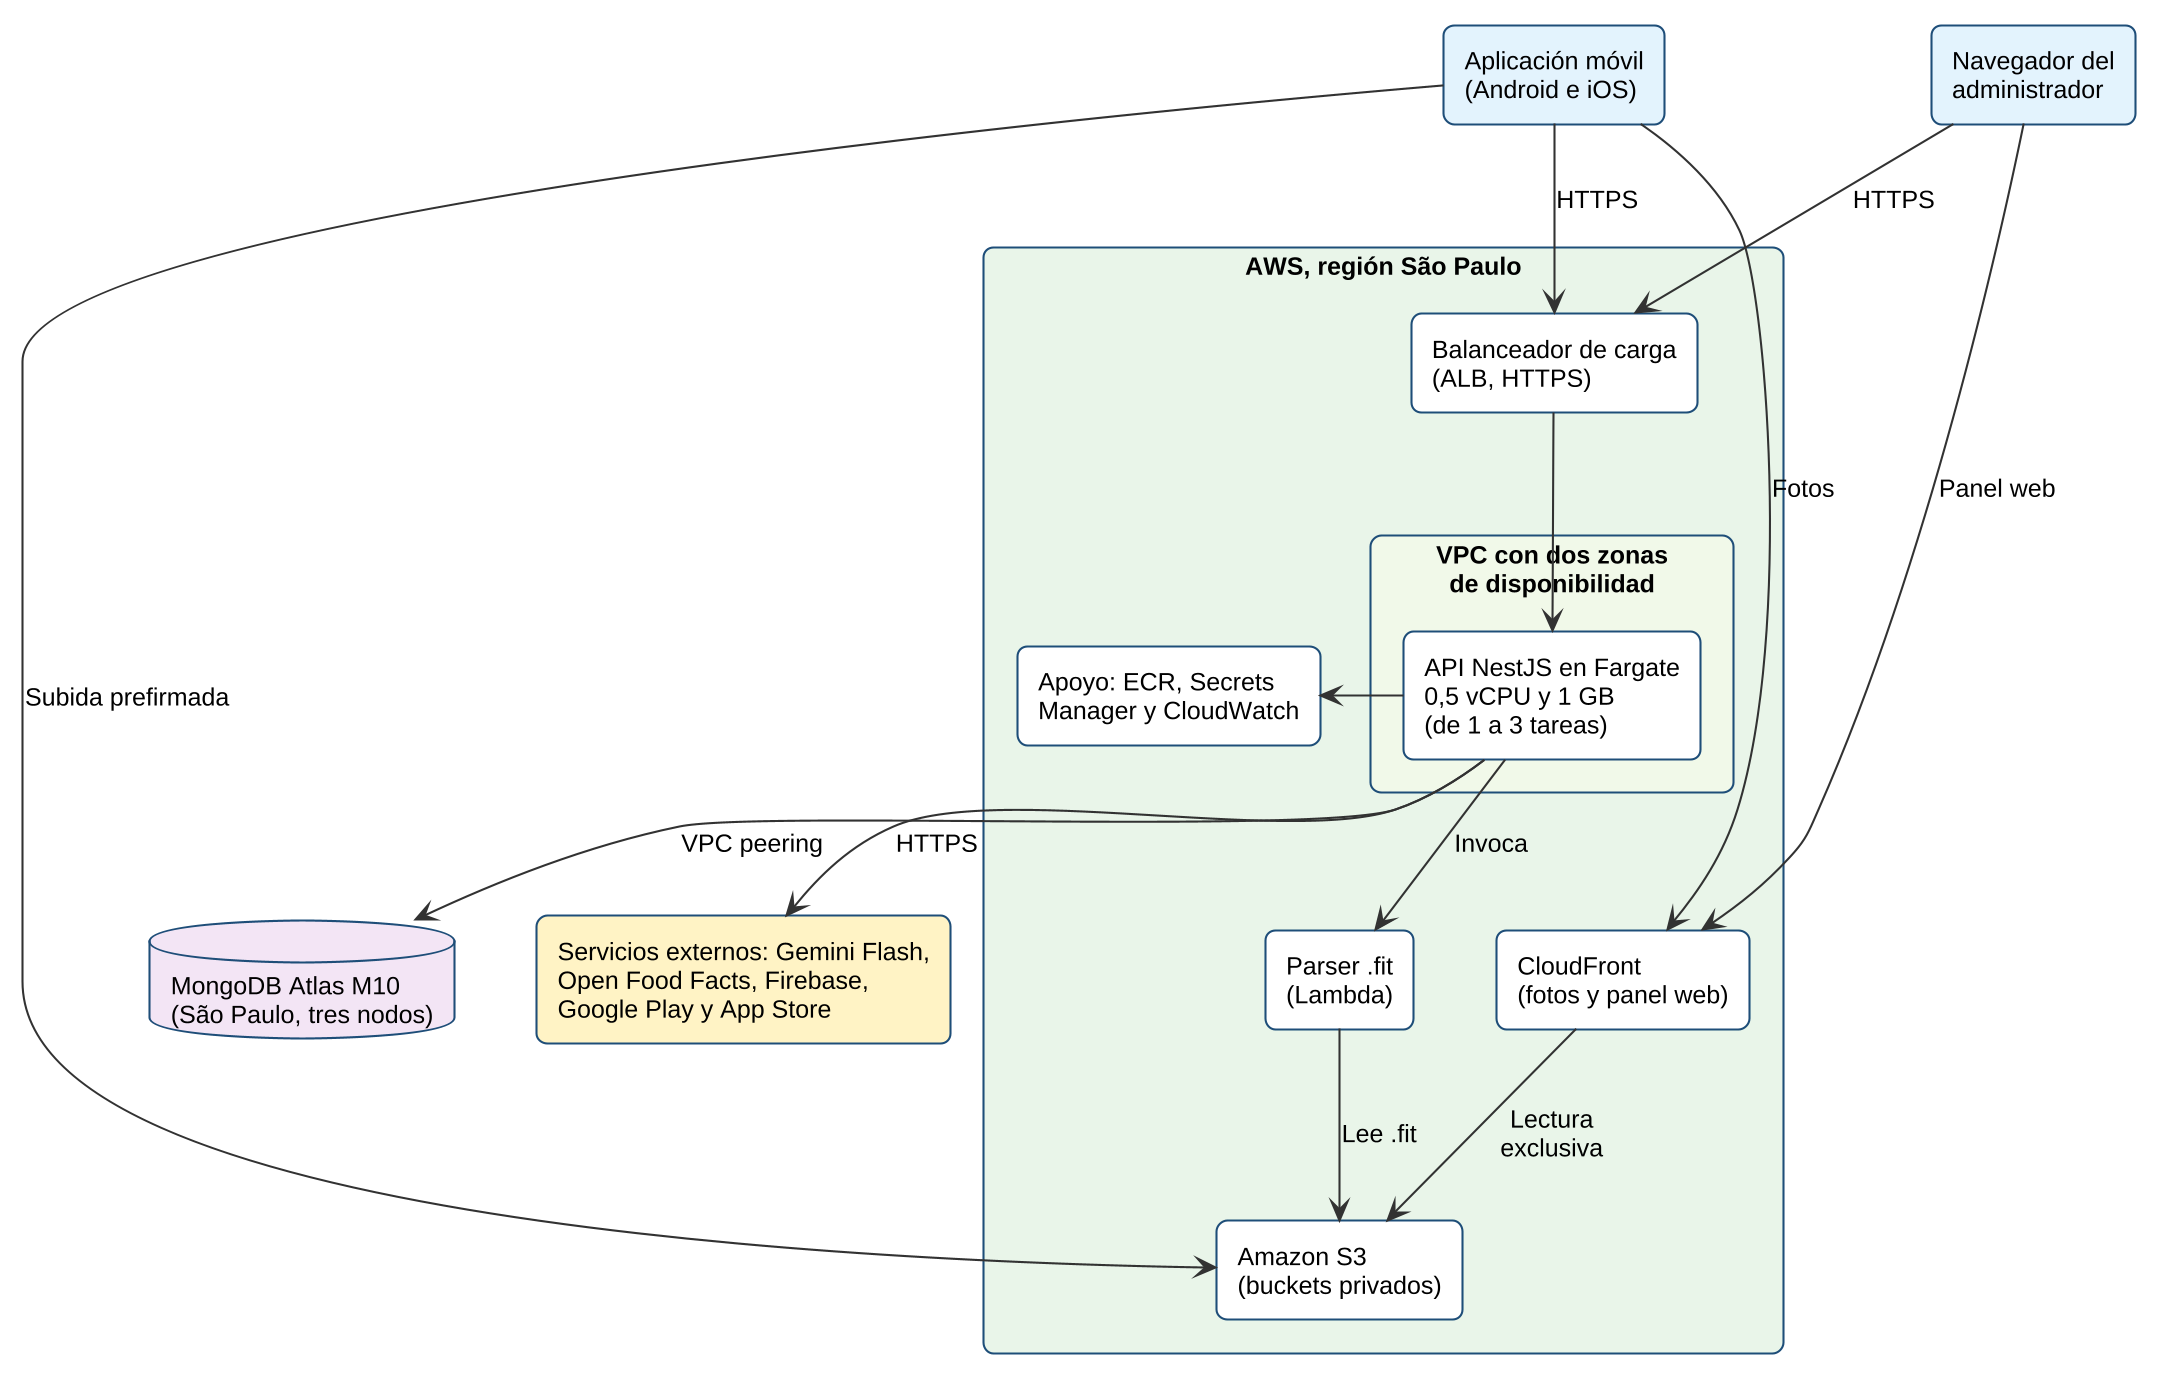
\includegraphics[width=0.95\textwidth,height=0.5\textheight,keepaspectratio]{figuras/arquitectura/arquitectura_detallada.png}
    \captionof{figure}{Arquitectura detallada de la solución.}
    \label{fig:arquitectura_detallada}
\end{center}

Las principales decisiones de esta arquitectura son las siguientes:

\begin{itemize}
    \item \textbf{Región de São Paulo:} Es la región de AWS más cercana con todos estos servicios, lo que reduce el tiempo de respuesta para usuarios en Chile. La base de datos está en la misma región.
    \item \textbf{API en Fargate:} Un contenedor pequeño alcanza para la carga esperada, y se agregan más cuando aumenta el uso. Para evitar el costo de una NAT Gateway, las tareas usan una IP pública, pero sus reglas de red solo aceptan tráfico entrante desde el balanceador.
    \item \textbf{Parser en Lambda:} Se esperan unos 20 archivos \texttt{.fit} al día, por lo que un contenedor encendido todo el tiempo estaría casi siempre sin hacer nada. Una función Lambda solo se ejecuta cuando llega un archivo.
    \item \textbf{MongoDB Atlas M10:} Es el nivel más bajo que permite una conexión privada con la red de AWS (VPC peering). Los datos de salud son sensibles, así que no conviene que la base de datos acepte conexiones desde cualquier dirección de Internet. Además, trae tres nodos con réplica y respaldos automáticos.
    \item \textbf{S3 y CloudFront:} Las fotos y los archivos no pasan por la API, como se explicó en la sección de integraciones.
\end{itemize}

\textbf{Carga esperada}

La Tabla \ref{tab:carga_esperada} muestra la carga estimada. Son supuestos que se deben confirmar con las pruebas de carga y con el uso real del prototipo.

\begin{table}[h!]
    \centering
    \renewcommand{\arraystretch}{1.25}
    \footnotesize
    \begin{tabular}{|>{\raggedright\arraybackslash}p{7.5cm}|>{\raggedright\arraybackslash}p{7.5cm}|}
        \hline
        \rowcolor[HTML]{EFEFEF}
        \textbf{Indicador} & \textbf{Valor estimado} \\ \hline
        Usuarios registrados & 1.500, de los cuales 159 son premium \\ \hline
        Usuarios activos al día & 600 (40\% de los registrados) \\ \hline
        Llamadas a la API al día & 24.000 (40 por usuario activo) \\ \hline
        Hora de mayor uso & 7.200 llamadas, 30\% del total del día \\ \hline
        Llamadas por segundo & 2 en promedio en la hora de mayor uso, y hasta 10 en momentos puntuales \\ \hline
        Archivos \texttt{.fit} al día & 20 (30\% de los premium, con 3 archivos a la semana) \\ \hline
        Fotos nuevas al mes & 7.200 (Tabla \ref{tab:costo_imagenes}) \\ \hline
    \end{tabular}
    \caption{Carga esperada del sistema.}
    \label{tab:carga_esperada}
\end{table}

\textbf{Almacenamiento}

La Tabla \ref{tab:almacenamiento} estima el espacio que usará MongoDB al cuarto año. La colección más grande es \texttt{telemetry}. Se asume que sus puntos ocupan 60 bytes cada uno y que las colecciones de series temporales de MongoDB los comprimen en un 70\%. Este último valor es un supuesto que se debe medir con datos reales.

\begin{table}[h!]
    \centering
    \renewcommand{\arraystretch}{1.25}
    \footnotesize
    \begin{tabular}{|>{\raggedright\arraybackslash}p{4cm}|r|>{\raggedright\arraybackslash}p{5.5cm}|r|}
        \hline
        \rowcolor[HTML]{EFEFEF}
        \textbf{Colección} & \textbf{Documentos} & \textbf{Cómo se calcula} & \textbf{Espacio} \\ \hline
        \texttt{telemetry} & 529 millones de puntos & Archivos \texttt{.fit} (1,5 horas, un punto por segundo) y rutas con GPS (1 hora, un punto cada 5 segundos) & 8,9 GB \\ \hline
        \texttt{meals} & 2,6 millones & 600 usuarios con 3 comidas al día, a 1,5 KB & 3,8 GB \\ \hline
        \texttt{workouts} & 499 mil & 600 usuarios con 4 sesiones a la semana, a 3 KB & 1,4 GB \\ \hline
        \texttt{dailyLogs} & 877 mil & 600 usuarios con un documento al día, a 1 KB & 0,8 GB \\ \hline
        \texttt{posts} y \texttt{fatigueSnapshots} & 405 mil & 3.600 publicaciones al mes y un cálculo diario por usuario premium & 0,5 GB \\ \hline
        Otras colecciones &  & Catálogos, rutinas, rutas, recetas y usuarios & 0,5 GB \\ \hline
        Índices &  & 25\% adicional sobre lo anterior & 4,0 GB \\ \hline
        \rowcolor[HTML]{E8F5E9}
        \textbf{Total} &  &  & \textbf{19,9 GB} \\ \hline
    \end{tabular}
    \caption{Almacenamiento estimado en MongoDB al cuarto año.}
    \label{tab:almacenamiento}
\end{table}

El primer año se usarían cerca de 5 GB, por lo que los 10 GB iniciales de un clúster M10 alcanzan durante los primeros dos años. Después, el almacenamiento se puede ampliar sin cambiar de nivel, ya que M10 permite hasta 128 GB \citep{atlas_pricing}. En Amazon S3 se acumularían unos 118 GB de fotos (Tabla \ref{tab:costo_imagenes}) y 29 GB de archivos \texttt{.fit} al cuarto año.
\textbf{Dimensionamiento por ambiente}

La Tabla \ref{tab:ambientes} muestra los recursos de cada ambiente. Como una sola persona desarrolla el proyecto, se usan tres ambientes simples. Los datos de prueba nunca se mezclan con los de producción.

\begin{table}[h!]
    \centering
    \renewcommand{\arraystretch}{1.25}
    \footnotesize
    \begin{tabular}{|>{\raggedright\arraybackslash}p{1.9cm}|>{\raggedright\arraybackslash}p{3.3cm}|>{\raggedright\arraybackslash}p{2.9cm}|>{\raggedright\arraybackslash}p{3.2cm}|>{\raggedright\arraybackslash}p{2.9cm}|}
        \hline
        \rowcolor[HTML]{EFEFEF}
        \textbf{Ambiente} & \textbf{Componente} & \textbf{Servicio} & \textbf{Capacidad} & \textbf{Observación} \\ \hline
        Producción & API & AWS Fargate & 0,5 vCPU y 1 GB, de 1 a 3 tareas & Agrega tareas si la CPU supera el 60\% \\ \hline
        Producción & Parser \texttt{.fit} & AWS Lambda & 1.769 MB de memoria & Se ejecuta solo al recibir un archivo \\ \hline
        Producción & Base de datos & MongoDB Atlas M10 & 2 vCPU, 2 GB de RAM y 10 GB, ampliable & Tres nodos con réplica \\ \hline
        Producción & Archivos y fotos & S3 y CloudFront & 118 GB de fotos y 29 GB de \texttt{.fit} al cuarto año & Buckets privados \\ \hline
        Producción & Balanceador & ALB & Dos zonas de disponibilidad & Certificado HTTPS \\ \hline
        QA & API & AWS Fargate & 0,25 vCPU y 0,5 GB, 1 tarea & Se enciende solo durante las pruebas \\ \hline
        QA & Base de datos & MongoDB Atlas M0 & 512 MB & Nivel gratuito, sin datos reales \\ \hline
        QA & Aplicación & Prueba interna de Google Play y TestFlight & Unos pocos usuarios & Evaluaciones del prototipo \\ \hline
        Desarrollo & API y base de datos & Docker en el computador & Según el computador & Sin costo de nube \\ \hline
        Desarrollo & Aplicación & Emulador o teléfono de prueba &  & Sin costo de nube \\ \hline
    \end{tabular}
    \caption{Dimensionamiento por ambiente.}
    \label{tab:ambientes}
\end{table}

La API se dimensionó con una tarea, porque la carga esperada es baja. Si esa tarea falla, AWS la reemplaza automáticamente, aunque el servicio puede quedar interrumpido por uno o dos minutos. Tener dos tareas permanentes evitaría esa interrupción, pero duplicaría el costo de este componente. Por eso se deja como una mejora para cuando la cantidad de usuarios lo justifique.
\textbf{Costo mensual de producción}

La Tabla \ref{tab:costo_produccion} muestra el costo de este dimensionamiento. Los precios de AWS son los publicados para la región de São Paulo \citep{aws_fargate_pricing}. MongoDB publica un valor de USD 57 al mes para M10 en Virginia \citep{atlas_pricing}, pero no se pudo confirmar el valor en São Paulo. Como los servicios de AWS cuestan cerca de un 70\% más en esa región, se considera USD 100 al mes, incluidos el almacenamiento y los respaldos. Este valor se debe confirmar antes de contratar el servicio.

\begin{table}[h!]
    \centering
    \renewcommand{\arraystretch}{1.25}
    \footnotesize
    \begin{tabular}{|>{\raggedright\arraybackslash}p{5cm}|>{\raggedright\arraybackslash}p{7.5cm}|r|}
        \hline
        \rowcolor[HTML]{EFEFEF}
        \textbf{Componente} & \textbf{Detalle} & \textbf{USD/mes} \\ \hline
        API en Fargate & 1 tarea de 0,5 vCPU y 1 GB, todo el mes & 31 \\ \hline
        Parser en Lambda & Dentro del nivel gratuito de AWS & 0 \\ \hline
        MongoDB Atlas M10 & Estimación para São Paulo & 100 \\ \hline
        Balanceador (ALB) & USD 0,034 por hora y uso bajo & 29 \\ \hline
        Direcciones IP públicas & 3 direcciones a USD 0,005 por hora & 11 \\ \hline
        CloudWatch & 5 GB de registros al mes & 5 \\ \hline
        S3 para archivos \texttt{.fit} & 29 GB al cuarto año, más solicitudes & 2 \\ \hline
        Fotos en S3 y CloudFront & Tabla \ref{tab:costo_imagenes} & 6 \\ \hline
        Secrets Manager, ECR y dominio & 6 secretos, 1 GB de imágenes y nombre de dominio & 4 \\ \hline
        \rowcolor[HTML]{E8F5E9}
        \textbf{Total} &  & \textbf{188} \\ \hline
    \end{tabular}
    \caption{Costo mensual estimado del ambiente de producción.}
    \label{tab:costo_produccion}
\end{table}

Este total es el que se usa en la factibilidad económica, donde corresponde a USD 182 al mes de infraestructura (Tabla \ref{tab:costo_infra}) y USD 6 al mes de imágenes (Tabla \ref{tab:costo_imagenes}). Con estos costos, y después de descontar el IVA, la comisión de las tiendas y el impuesto a la renta, la Alternativa 3 necesita 159 suscriptores para alcanzar el equilibrio.
\textbf{Cuándo aumentar la capacidad}

La Tabla \ref{tab:escalamiento} indica qué señal avisa que se debe ampliar cada componente.

\begin{table}[h!]
    \centering
    \renewcommand{\arraystretch}{1.25}
    \footnotesize
    \begin{tabular}{|>{\raggedright\arraybackslash}p{3.5cm}|>{\raggedright\arraybackslash}p{5.7cm}|>{\raggedright\arraybackslash}p{5.7cm}|}
        \hline
        \rowcolor[HTML]{EFEFEF}
        \textbf{Componente} & \textbf{Señal} & \textbf{Acción} \\ \hline
        API & La CPU supera el 60\% durante varios minutos & Agregar tareas automáticamente, hasta 3. Si no alcanza, subir la capacidad de cada tarea \\ \hline
        Base de datos & La memoria o la CPU se mantienen altas & Pasar de M10 a M20 \\ \hline
        Almacenamiento & Se usa más del 80\% del espacio & Ampliar el disco del clúster \\ \hline
        Entrega de fotos & Se acerca a 1 TB al mes & Pagar el exceso sobre el nivel gratuito de CloudFront \\ \hline
    \end{tabular}
    \caption{Señales para aumentar la capacidad.}
    \label{tab:escalamiento}
\end{table}
\subsection{Diagrama de Despliegue}
La Figura \ref{fig:diagrama_despliegue} muestra dónde se instala cada parte del sistema y cómo se comunican.
\begin{center}
    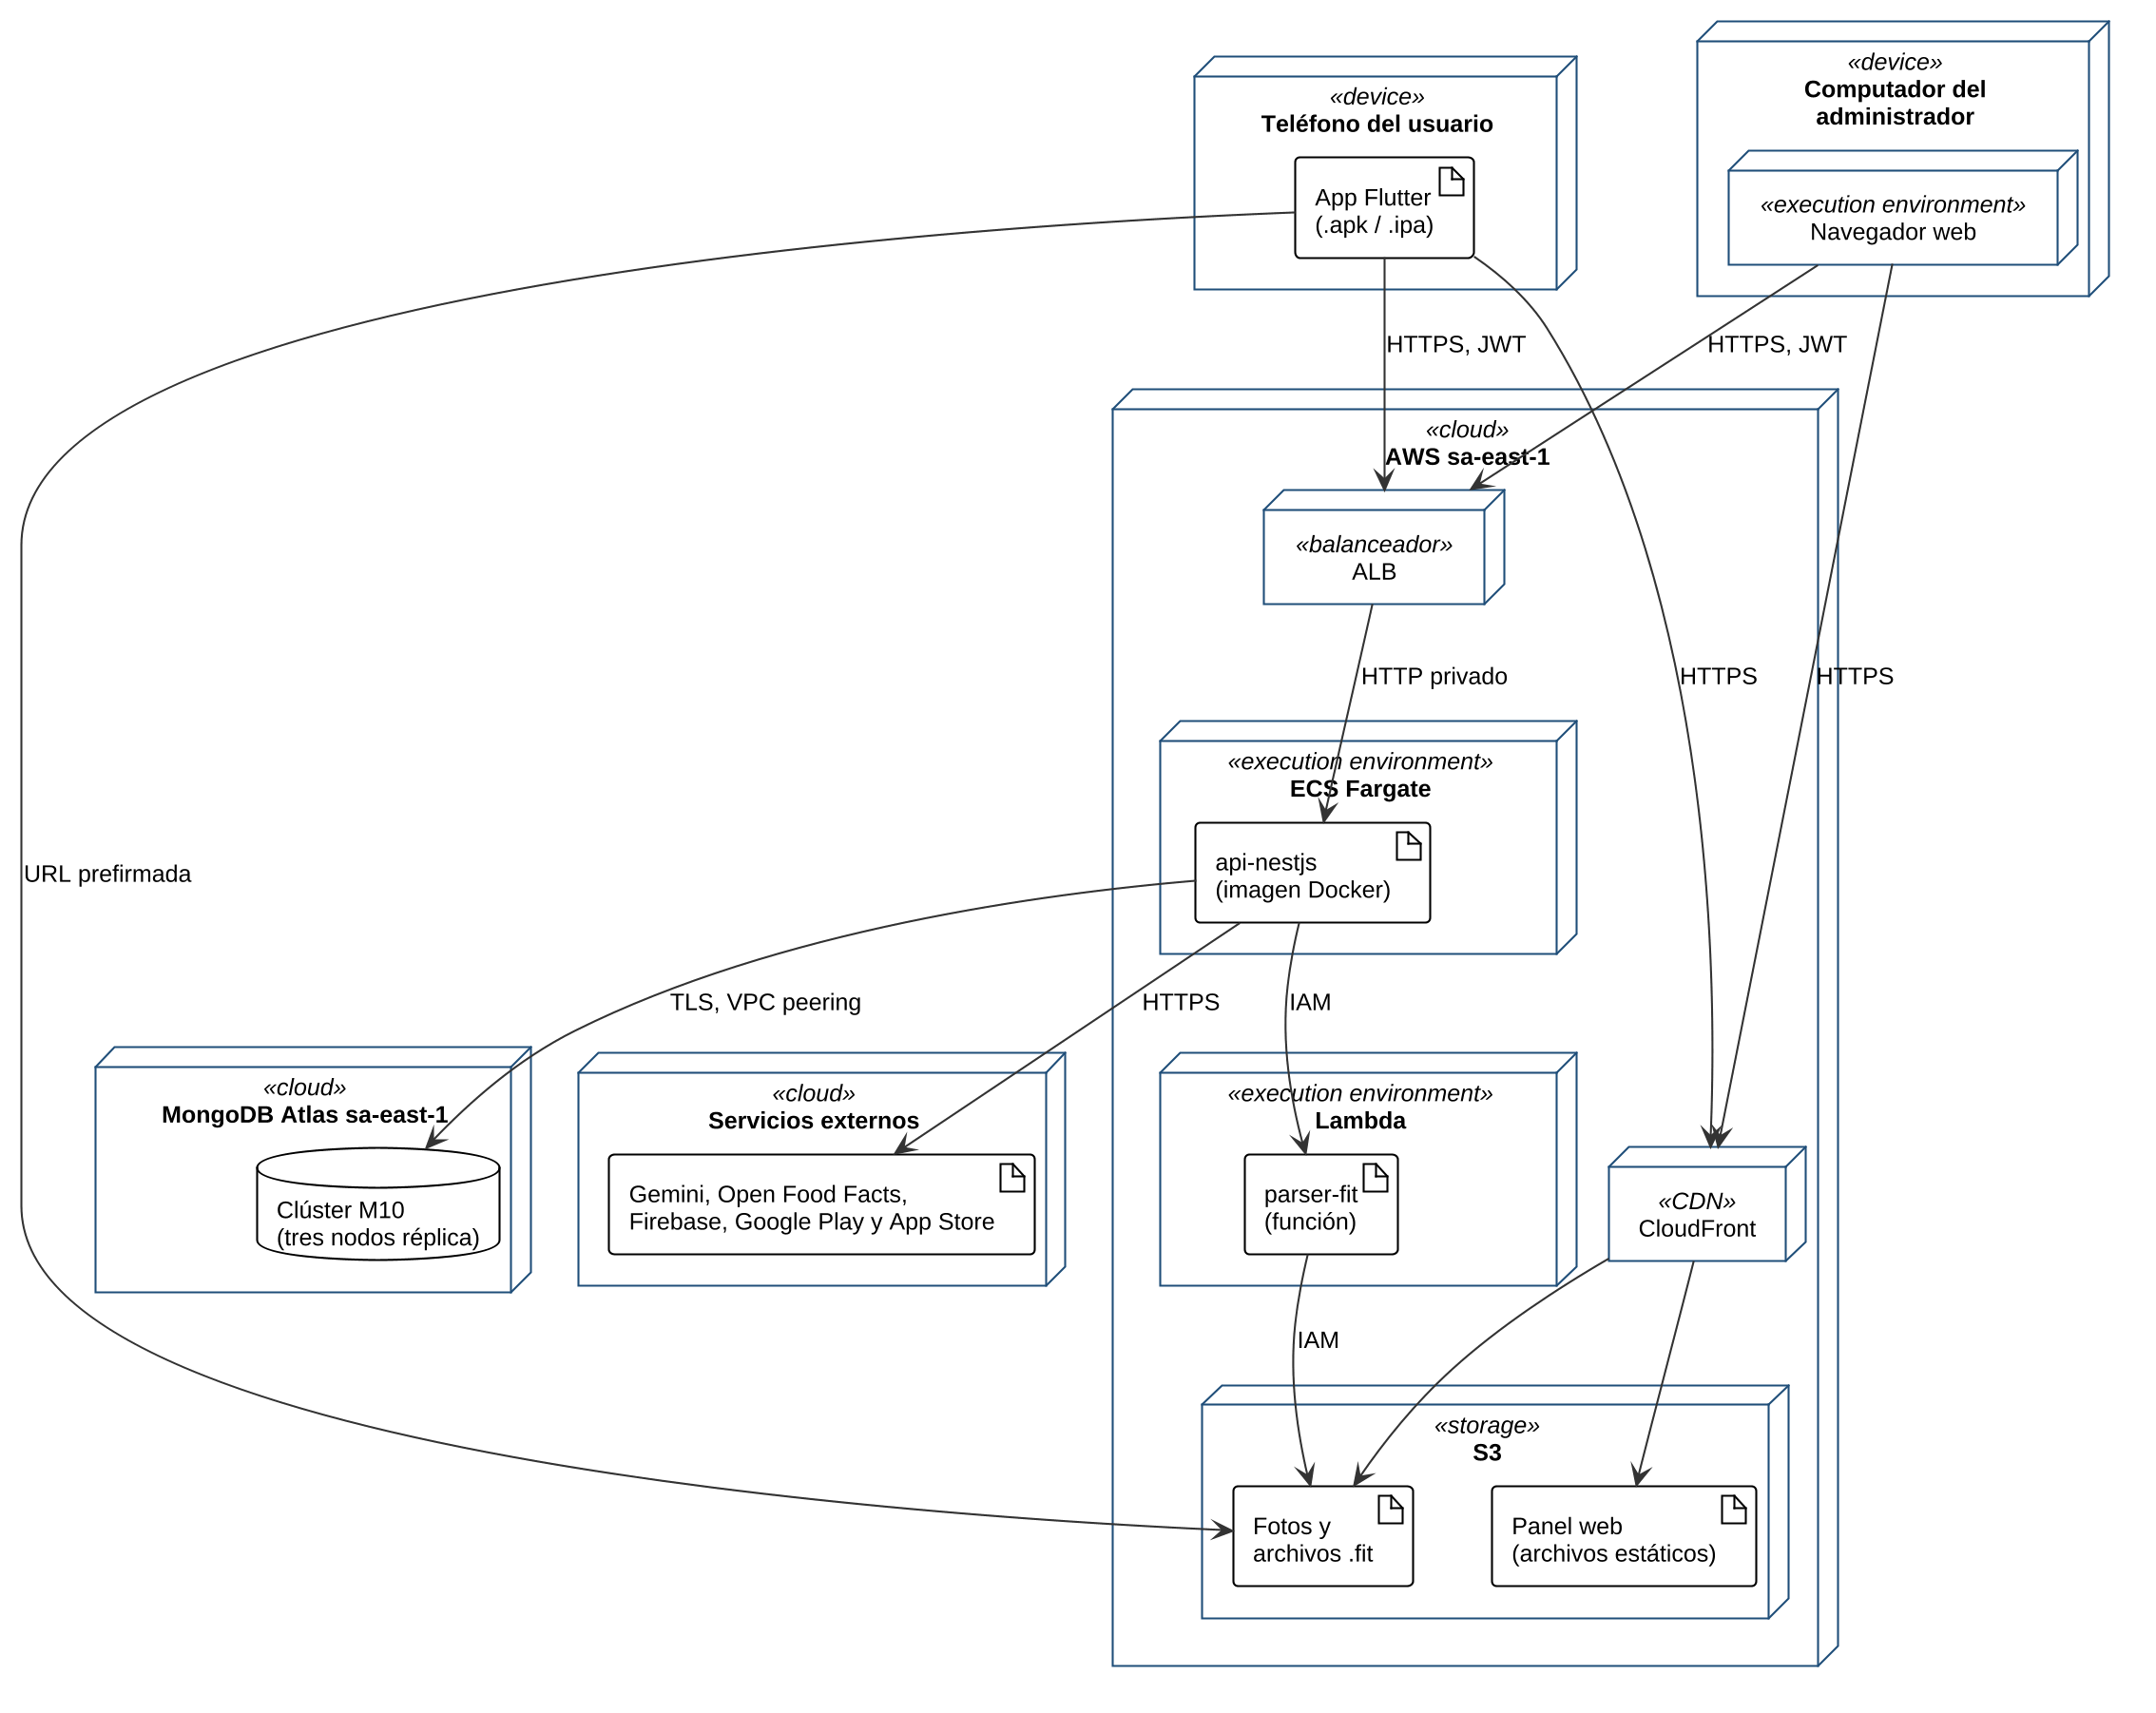
\includegraphics[width=0.9\textwidth,height=0.55\textheight,keepaspectratio]{figuras/arquitectura/diagrama_despliegue.png}
    \captionof{figure}{Diagrama de despliegue de la solución.}
    \label{fig:diagrama_despliegue}
\end{center}

El sistema se compone de cuatro piezas que se instalan por separado:

\begin{itemize}
    \item \textbf{Aplicación móvil:} Se compila desde un solo código en Flutter y se publica en Google Play (\texttt{.apk}) y en App Store (\texttt{.ipa}). Cada usuario la instala en su teléfono.
    \item \textbf{API:} Se empaqueta como una imagen Docker, que se guarda en Amazon ECR y se ejecuta en ECS Fargate. Para actualizarla, se inicia una tarea con la versión nueva y luego se apaga la anterior, de modo que el servicio no se interrumpe.
    \item \textbf{Parser \texttt{.fit}:} Se publica como una función de AWS Lambda. Solo la API puede invocarla, y solo tiene permiso para leer el bucket de archivos.
    \item \textbf{Panel web:} Son archivos estáticos que se guardan en S3 y se entregan a través de CloudFront. El administrador lo abre desde su navegador.
\end{itemize}

MongoDB Atlas lo opera su proveedor, por lo que no hay que instalar el motor de base de datos. Se debe crear el clúster, configurar la conexión privada con la red de AWS y definir los índices descritos en el modelo de datos. Las claves de los servicios externos se guardan en AWS Secrets Manager y no quedan en el código ni en la imagen Docker.
\begin{spacing}{1.0}
\subsection{Comentarios Generales del Capítulo}
En este capítulo se definió cómo se va a construir la solución. A partir de los requerimientos del capítulo anterior, se describió cada caso de uso con sus precondiciones, sus flujos y su diagrama de actividades, y se detalló su funcionamiento técnico con un diagrama de secuencia. También se diseñó el modelo de datos en MongoDB, las interfaces de usuario de cada caso de uso, las integraciones con los seis sistemas externos, la infraestructura y su despliegue.

\medskip
El diseño dejó dos aportes principales. El primero es que aclaró lo que faltaba. Al trazar cada caso de uso paso a paso, se encontraron datos necesarios que el modelo no tenía, como el registro de quién reporta una publicación, y se corrigieron antes de programar. El segundo es que se comprobaron los costos. Al dimensionar la infraestructura con precios reales de AWS en São Paulo, se vio que la estimación inicial era baja, lo que llevó a ajustar la factibilidad económica. Sumando el IVA, la comisión de las tiendas y el impuesto a la renta, la solución elegida necesita 159 suscriptores. También se tomaron decisiones para gastar solo en lo necesario, como usar una función Lambda para leer archivos \texttt{.fit} y subir las fotos directamente a Amazon S3, sin dejar de proteger los datos sensibles con una conexión privada a la base de datos.

\medskip
Algunos valores de este diseño todavía son supuestos que se deben confirmar, como la carga esperada, la compresión de los datos de telemetría y el precio de MongoDB Atlas en São Paulo. Esto es parte del prototipo evolutivo, ya que cada versión permitirá medir estos valores y ajustar el diseño. Lo mismo ocurre con las interfaces de usuario, ya que varias pantallas muestran por ahora datos simulados y se conectarán a medida que se implementen sus servicios. Con este capítulo quedan cumplidos los objetivos específicos 1 a 4, según los criterios de la Tabla \ref{tab:validacion}. El objetivo 5, que es implementar el MVP y verificar el cruce de datos, corresponde a la etapa siguiente. Para ello ya existe un prototipo funcional en iOS que implementa el registro de fuerza, el registro de cardio con GPS y la nutrición, además del cálculo de la carga y de la fatiga cruzada definido en el Capítulo 3, con pruebas unitarias. Con esta base, el proyecto puede avanzar a la implementación, donde se planifica la puesta en marcha y las pruebas del sistema.
\end{spacing}
